\documentclass[twoside,12pt]{Classes/PhDThesis}
\newcommand{\cmsSymbolFace}{\mathrm}

\newcommand{\lumi}{\ensuremath{\mathcal{L}}\xspace}
\newcommand{\lumiint}{\ensuremath{\mathcal{L}_{\textrm{int}}}\xspace}
\newcommand {\Et}{$\textrm{E}_{\textrm{T}}$\hspace{1mm}}
\newcommand {\Etj}{$\textrm{E}_{\textrm{T}}(\textrm{jet})$\hspace{1mm}}
\newcommand {\mva}{$d_{\textrm{MVA}}$\hspace{1mm}}
\newcommand {\mvat}{$d^{thresh.}_{\textrm{MVA}}$\hspace{1mm}}
\newcommand {\etrue}{$\epsilon^{\textrm{true}}_{\textrm{QCD}}$\hspace{1mm}}
\newcommand {\est}{$\epsilon^{\textrm{est.}}_{\textrm{QCD}}$\hspace{1mm}}
% Physics symbols ...from pdefs
\newcommand{\PT}{\ensuremath{p_{\mathrm{T}}}\xspace}
\newcommand{\pt}{\ensuremath{p_{\mathrm{T}}}\xspace}
\newcommand{\pthat}{\ensuremath{\hat{p}_{\mathrm{T}}}\xspace}
\newcommand{\pz}{\ensuremath{p_{\mathrm{z}}}\xspace}
\newcommand{\ptm}{\ensuremath{\pt(\mu)}\xspace}
\newcommand{\ET}{\ensuremath{E_{\mathrm{T}}}\xspace}
\newcommand{\HT}{\ensuremath{H_{\mathrm{T}}}\xspace}
\newcommand{\et}{\ensuremath{E_{\mathrm{T}}}\xspace}
\newcommand{\ETm}{\ensuremath{E_{\mathrm{T}}^{\textrm{miss}}}\xspace}
\newcommand{\Exm}{\ensuremath{E_{x}^{\textrm{miss}}}\xspace}
\newcommand{\Eym}{\ensuremath{E_{y}^{\textrm{miss}}}\xspace}
\newcommand{\vecETm}{\ensuremath{\vec{E}_{\mathrm{T}}^{\textrm{miss}}}\xspace}
\newcommand{\ETmsquared}{\ensuremath{E_{\mathrm{T}}^{\textrm{miss } 2}}\xspace}
\newcommand{\MET}{\ETm}
\newcommand{\METvec}{\ensuremath{\vec{E}_\mathrm{T}^\textrm{miss}}\xspace}
\newcommand{\ETmiss}{\ETm}
\newcommand{\met}{\ETm}
\newcommand{\mex}{\Exm}
\newcommand{\mey}{\Eym}
\newcommand{\vecmet}{\vecETm}
\newcommand{\metsquared}{\ETmsquared}

\newcommand{\st}{\ensuremath{S_{\mathrm{T}}}\xspace}
\newcommand{\mt}{\ensuremath{M_\mathrm{T}^{\mathrm{W}}}\xspace}
\newcommand{\wpt}{\ensuremath{p_\mathrm{T}^{\mathrm{W}}}\xspace}
\newcommand{\ST}{\st}
\newcommand{\MT}{\mt}
\newcommand{\WPT}{\wpt}

%particles
\newcommand{\proton}{\ensuremath{\cmsSymbolFace{p}}\xspace}
\newcommand{\cPqt}{\ensuremath{\cmsSymbolFace{t}}\xspace} % t for t quark
\newcommand{\cPqb}{\ensuremath{\cmsSymbolFace{b}}\xspace} % b for b quark
\newcommand{\cPqc}{\ensuremath{\cmsSymbolFace{c}}\xspace} % c for c quark
\newcommand{\cPqs}{\ensuremath{\cmsSymbolFace{s}}\xspace} % s for s quark
\newcommand{\cPqu}{\ensuremath{\cmsSymbolFace{u}}\xspace} % u for u quark
\newcommand{\cPqd}{\ensuremath{\cmsSymbolFace{d}}\xspace} % d for d quark
\newcommand{\cPq}{\ensuremath{\cmsSymbolFace{q}}\xspace} % generic quark
\newcommand{\cPaqt}{\ensuremath{\overline{\cmsSymbolFace{t}}}\xspace} % t for t anti-quark
\newcommand{\cPaqb}{\ensuremath{\overline{\cmsSymbolFace{b}}}\xspace} % b for b anti-quark
\newcommand{\cPaqc}{\ensuremath{\overline{\cmsSymbolFace{c}}}\xspace} % c for c anti-quark
\newcommand{\cPaqs}{\ensuremath{\overline{\cmsSymbolFace{s}}}\xspace} % s for s anti-quark
\newcommand{\cPaqu}{\ensuremath{\overline{\cmsSymbolFace{u}}}\xspace} % u for u anti-quark
\newcommand{\cPaqd}{\ensuremath{\overline{\cmsSymbolFace{d}}}\xspace} % d for d anti-quark
\newcommand{\cPaq}{\ensuremath{\overline{\cmsSymbolFace{q}}}\xspace} % generic anti-quark
\newcommand{\cPg}{\ensuremath{\cmsSymbolFace{g}}\xspace} % generic gluon
\newcommand{\cPG}{\ensuremath{\cmsSymbolFace{G}}\xspace} % Graviton
\newcommand{\zp}{\ensuremath{\cmsSymbolFace{Z}^\prime}\xspace} % plain Z'
\newcommand{\Z}{\ensuremath{\cmsSymbolFace{Z}}\xspace} % plain Z (no superscript 0)
\newcommand{\ZpJets}{\ensuremath{\Z+\textrm{jets}}\xspace}
\newcommand{\W}{\ensuremath{\cmsSymbolFace{W}}\xspace}
\newcommand{\WpJets}{\ensuremath{\W+\textrm{jets}}\xspace}
\newcommand{\VpJets}{\ensuremath{\cmsSymbolFace{V}+\textrm{jets}}\xspace}
\providecommand{\PH}{\ensuremath{\cmsSymbolFace{H}}\xspace} % plain Higgs
\newcommand{\cPqst}{\ensuremath{\widetilde{\cPqt}}\xspace} % t for stop quark
\newcommand{\JPsi}{\ensuremath{\cmsSymbolFace{J}\hspace{-.08em}/\hspace{-.14em}\psi}\xspace} % J/Psi (no mass)
\newcommand{\photon}{\ensuremath{\gamma}\xspace} % plain Z (no superscript 0)
\newcommand{\tW}{\ensuremath{\cmsSymbolFace{t}\cmsSymbolFace{W}}\xspace}

\newcommand{\qqbar}{\ensuremath{\cmsSymbolFace{q}\overline{\cmsSymbolFace{q}}}\xspace} % q-qbar
\newcommand{\ttbar}{\ensuremath{\cmsSymbolFace{t}\overline{\cmsSymbolFace{t}}}\xspace} % t-tbar
\newcommand{\ttjets}{\ensuremath{\cmsSymbolFace{t}\overline{\cmsSymbolFace{t}}+\textrm{jets}}\xspace} % ttjets
\newcommand{\sigttbar}{\ensuremath{\sigma_{\ttbar}}}
%from pdefs END
\newcommand{\tquark}{\ensuremath{\cPqt\textrm{-quark}}\xspace}
\newcommand{\tquarks}{\ensuremath{\cPqt\textrm{-quarks}}\xspace}
\newcommand{\bquark}{\ensuremath{\cPqb\textrm{-quark}}\xspace}
\newcommand{\bquarks}{\ensuremath{\cPqb\textrm{-quarks}}\xspace}
\newcommand{\cquark}{\ensuremath{\cPqc\textrm{-quark}}\xspace}
\newcommand{\cquarks}{\ensuremath{\cPqc\textrm{-quarks}}\xspace}
%new since ttbar + MET
% \newcommand{\mtt}{m$_{\ttbar}$~}
\newcommand{\mtt}{\ensuremath{m_{\ttbar}}\xspace}
\newcommand{\mttbar}{\mtt}
\newcommand{\mtop}{\ensuremath{m_\cPqt}\xspace}
\newcommand{\MSmtop}{\ensuremath{\overline{m}_\cPqt}\xspace}
\newcommand{\MS}{\ensuremath{\overline{\textrm{MS}}}\xspace}
\newcommand{\qq}{$\mathrm{q}\bar{\mathrm{q}}$~}
\newcommand{\xsect}{cross section\xspace} % with or without a hyphen? Make sure it agrees with the usage in the abstract (above)
\newcommand{\xSect}{Cross section} % with an initial capital, but with or without a hyphen?
\newcommand{\CoM}{centre of mass\xspace}
\newcommand{\Nttbar}{N_{\mathrm{t}\overline{\mathrm{t}}}}
\newcommand{\rec}{\mathrm{rec}}
\newcommand{\gen}{\mathrm{gen}}
\newcommand{\MTW}{\ensuremath{M_T(\W)}\xspace}

%unit abbrevations
\newcommand{\pb}{\pico\barn}
\newcommand{\fb}{\femto\barn}
\newcommand{\pbinv}{\ensuremath{\textrm{\pb}^{-1}}}
\newcommand{\fbinv}{\ensuremath{\textrm{\fb}^{-1}}}

%generators from pdefs
\newcommand{\GEANT}{{\textsc{GEANT}}\xspace}
\newcommand{\GEANTfour}{{\textsc{Geant4}}\xspace}
\newcommand{\HERWIG}{{\textsc{HERWIG}}\xspace}
\newcommand{\MADGRAPH}{\textsc{MadGraph}\xspace}
\newcommand{\MCATNLO} {\textsc{MC@NLO}\xspace}
\newcommand{\MCFM} {\textsc{MCFM}\xspace}
\newcommand{\POWHEG} {{\textsc{POWHEG}}\xspace}
\newcommand{\PYTHIA} {{\textsc{PYTHIA}}\xspace}
\newcommand{\SHERPA} {{\textsc{SHERPA}}\xspace}
\newcommand{\TAUOLA} {\textsc{TAUOLA}\xspace}
\newcommand{\RAW} {\textsc{RAW}\xspace}
\newcommand{\RECO} {\textsc{RECO}\xspace}
\newcommand{\AOD} {\textsc{AOD}\xspace}
%other stuff from pdefs
% \newcommand{\CMSSW} {\ensuremath{\textrm{\verb+CMSSW}}}
\newcommand{\CMSSW}{\textsc{CMSSW}\xspace}
\newcommand{\ROOT}{\textsc{ROOT}\xspace}
\newcommand{\Lone}{Level-1\xspace}
\newcommand{\Tevatron}{Tevatron\xspace}
\newcommand{\Dzero}{D{\O}\xspace}
\newcommand{\HitFit}{\textsc{HitFit}\xspace}
\newcommand{\Cplusplus}{\textsc{C}\texttt{++}\xspace}

\newcommand {\ie}{\mbox{i.e.}\xspace}     %i.e.
\newcommand {\eg}{\mbox{e.g.}\xspace}     %e.g.
\newcommand {\etc}{\mbox{etc.}\xspace}     %etc.
\newcommand {\vs}{\mbox{\sl vs.}\xspace}      %vs.
\newcommand {\mdash}{\ensuremath{\mathrm{-}}} % for use within formulas
\newcommand{\calL}{\mathcal{L}}
\newcommand{\cL}{\mathcal{L}}
\newcommand{\twovector}[2]{\begin{pmatrix} #1 \\ #2 \end{pmatrix}}
\newcommand{\threevector}[3]{\begin{pmatrix} #1 \\ #2 \\ #3 \end{pmatrix}}
\newcommand{\bigO}{\ensuremath{\mathcal{O}}}

\newcommand{\stat}{\ensuremath{\,\textrm{(stat.)}}\xspace}
\newcommand{\syst}{\ensuremath{\,\textrm{(syst.)}}\xspace}

\newcommand{\DR}{\ensuremath{\Delta R}}
%from pdefs (adding a touch of SIunitx) 
%unit abbrevations
\DeclareSIUnit\micron{\micro\metre}
\DeclareSIUnit\mrad{\milli\rad}
\DeclareSIUnit\gauss{G}
\DeclareSIUnit\eVperc{\eV\per\clight}
\DeclareSIUnit\nanobarn{\nano\barn}
\DeclareSIUnit\picobarn{\pico\barn}
\DeclareSIUnit\femtobarn{\femto\barn}
\DeclareSIUnit\attobarn{\atto\barn}
\DeclareSIUnit\zeptobarn{\zepto\barn}
\DeclareSIUnit\yoctobarn{\yocto\barn}
\DeclareSIUnit\nb{\nano\barn}
\DeclareSIUnit\pb{\pico\barn}
\DeclareSIUnit\fb{\femto\barn}
\DeclareSIUnit\invpb{\per\pico\barn}
\DeclareSIUnit\invfb{\per\femto\barn}
\DeclareSIUnit\ab{\atto\barn}
\DeclareSIUnit\zb{\zepto\barn}
\DeclareSIUnit\yb{\yocto\barn}
% \newcommand{\micron}{\micro\meter}%this is causing corrupt NFSS tables
% \renewcommand{\micron}{\ensuremath{\mu}\meter}
% roman face derivative
\newcommand{\dd}[2]{\ensuremath{\frac{\cmsSymbolFace{d} #1}{\cmsSymbolFace{d} #2}}}
\newcommand{\ddinline}[2]{\ensuremath{\cmsSymbolFace{d} #1/\cmsSymbolFace{d} #2}}
\newcommand{\rd}{\ensuremath{\cmsSymbolFace{d}}}
% absolute value
\newcommand{\abs}[1]{\ensuremath{\lvert #1 \rvert}}
\newcommand{\alpS}{\ensuremath{\alpha_S}\xspace}
\newcommand{\kt}{\ensuremath{k_{\mathrm{t}}}\xspace}
\newcommand{\antikt}{\ensuremath{\mathrm{anti}\textrm{-}k_{\mathrm{t}}}\xspace}
\newcommand{\pc}{\%}

%triggers

%\newcommand{\HLTThreeCentralJetNonIso}{HLT-Ele25-CaloIdVT-TrkIdT-TriCentralJet30 \xspace}
%\newcommand{\HLTThreeCentralJet}{HLT-Ele25-CaloIdVT-CaloIsoT-TrkIdT-TrkIsoT-TriCentralJet30}
%\newcommand{\HLTThreeCentralPFJet}{HLT-Ele25-CaloIdVT-CaloIsoT-TrkIdT-TrkIsoT-TriCentralPFJet30 \xspace}
\newcommand{\HLTThreeCentralJet}{HLT\_Ele25\_CaloIdVT\_CaloIsoT\_TrkIdT\_TrkIsoT\_TriCentralJet30\xspace}
\newcommand{\HLTThreeCentralPFJet}{HLT\_Ele25\_CaloIdVT\_CaloIsoT\_TrkIdT\_TrkIsoT\_TriCentralPFJet30\xspace}

\newcommand{\reliso}{\ensuremath{\textrm{reliso}}\xspace}
\newcommand{\bjet}{\ensuremath{\textrm{\cPqb-jet}}\xspace}
\newcommand{\btag}{\ensuremath{\textrm{\cPqb-tag}}\xspace}
\newcommand{\btags}{\ensuremath{\textrm{\cPqb-tags}}\xspace}
\newcommand{\btagging}{\ensuremath{\textrm{\cPqb-tagging}}\xspace}
\newcommand{\btagged}{\ensuremath{\textrm{\cPqb-tagged}}\xspace}
\newcommand{\pdf}{\ensuremath{\mathrm{pdf}}}
\newcommand{\multijet}{multi-jet}
\newcommand{\eplusjets}{electron channel}
\newcommand{\muplusjets}{muon channel}

\newcommand{\Niexp}{\ensuremath{N_i^\textrm{exp}}}
\newcommand{\Niobs}{\ensuremath{N_i^\textrm{obs}}}

 
\ifpdf
    \pdfinfo { /Title  (PhD Thesis)
               /Creator (TeX)
               /Producer (pdfTeX)
               /Author (Sergey Senkin sergey.senkin@bristol.ac.uk)
               /CreationDate (D:20130123000000)  %format D:YYYYMMDDhhmmss
               /ModDate (D:20130123000000)
               /Subject (PhD Thesis)
               /Keywords (Bristol, phd, thesis, top, quark)}
    \pdfcatalog { /PageMode (/UseOutlines)
                  /OpenAction (fitbh)  }
\fi

\title{Top Quark Physics at the LHC \\ with the CMS Detector  \\[1ex]
        }

\ifpdf
  \author{\href{mailto:sergey.senkin@bristol.ac.uk}{Sergey Senkin}}
  \collegeordept{\href{http://www.phy.bris.ac.uk/}{School of Physics}}
  \university{\href{http://www.bristol.ac.uk}{University of Bristol}}
  \crest{
\includegraphics[width=60mm]{UnivShield}}
\else
  \author{Sergey Senkin}
  \collegeordept{School of Physics}
  \university{University of Bristol}
  \crest{
\includegraphics[bb = 0 0 292 336, width=60mm]{UnivShield}}
\fi

\renewcommand{\submittedtext}{\textit{A dissertation submitted to the University
of Bristol \\ in accordance with the requirements of the degree of \\ Doctor of
Philosophy in the Faculty of Science}}
\degree{}
\degreedate{\today}

% turn of those nasty overfull and underfull hboxes
\hbadness=10000
\hfuzz=50pt

% setup the SIunits package (more info in 'texdoc siunitx')
\sisetup{number-unit-product = \text{ }}
\sisetup{binary-units = true}
\sisetup{seperr, openerr=, closeerr=}

% Print URLs not in Typewriter Font                                     
\def\UrlFont{\rm}

% Put all the style files you want in the directory StyleFiles and usepackage like this:
%\usepackage{StyleFiles/watermark}

\addbibresource{References/references.bib}

\begin{document}
%roman page numbering for Title page, abstract and index
\pagenumbering{roman}

%\watermark{DRAFT COPY}

%\onehalfspacing

\maketitle

%set the number of sectioning levels that get number and appear in the contents
\setcounter{secnumdepth}{3}
\setcounter{tocdepth}{3}

\frontmatter % book mode only
%% Thesis Dedictation ---------------------------------------------------

\begin{dedication} %this creates the heading for the dedication page

\textit{To my parents}

\end{dedication}

% ----------------------------------------------------------------------

%%% Local Variables: 
%%% mode: latex
%%% TeX-master: "../thesis"
%%% End: 

%
% Thesis Abstract -----------------------------------------------------

\begin{abstract}        %this creates the heading for the abstract page
In this thesis, the top quark mass and top quark pair differential cross section measurements in the lepton plus jets
channel are presented.
\end{abstract}
%%!TEX root = ../thesis.tex

% Thesis Acknowledgements ------------------------------------------------


\begin{acknowledgements}
The past three and a half years have been a challenging yet extremely rewarding experience. Quite a few people have made
it possible, and I am incredibly grateful to all of them. First of all, I would like to thank my supervisor, Greg Heath,
for his valuable guidance, advice and constructive suggestions, especially in writing up this thesis. I also thank Joel
Goldstein for leading the research group and being a wise and kind host to our weekly meetings. Your advice has been
greatly appreciated.

This work would not have been possible without some serious funding. I would like to thank the Faculty of Science and
the selection panel for awarding me the University of Bristol Postgraduate Research Scholarship. It has been a great
honour and I hope I managed to live up to it. I'm also very thankful to Dave Newbold (and Joel, again) for arranging the
additional funding for my work at CERN, as otherwise my time there would have been rather miserable despite the great
privilege of witnessing the Higgs boson discovery.

Many thanks to Jeson Jacob, \L{}ukasz Kreczko and Phil Symonds for being great teammates over the last few years. I am
particularly grateful to Luke who has been a nearly endless source of knowledge, and always willing to help. K-thx-bye!

A number of people helped me during my placement at CERN. In particular, I would like to thank Martijn Mulders and
Enrique Palencia for their collaboration and helpful advice on the top mass analysis. My work on the high-level trigger
was greatly influenced by St\'{e}phanie Beauceron and Sam Harper -- thank you for the guidance and useful advice. And
special thanks to the UK Liaison Office at CERN for helping me deal with the French bureaucracy.

I would also like to express my gratitude to Alexei Safonov and Jim Pivarski for introducing me to CMS back in 2008, and
giving me a chance to appreciate and get inspired by the collaboration spirit. Thank you, without your help and good
will this PhD would not have been possible.

My warmest thanks go to all my friends and family, and especially to my parents. Your continuous encouragement and
support throughout all this time have been immensely appreciated.

\end{acknowledgements}

% ------------------------------------------------------------------------

%%% Local Variables: 
%%% mode: latex
%%% TeX-master: "../thesis"
%%% End: 

%% Thesis Declaration ---------------------------------------------------

\begin{declaration}

I declare that the work in this dissertation was carried out in accordance with the requirements of the University's
Regulations and Code of Practice for Research Degree Programmes and that it has not been submitted for any other
academic award. Except where indicated by specific reference in the text, the work is the candidate's own work. Work
done in collaboration with, or with the assistance of, others, is indicated as such. Any views expressed in the
dissertation are those of the author.

\vspace{5cm}

Signed:\ldots\ldots\ldots\ldots\ldots\ldots\ldots\ldots \hfill
Date:\ldots\ldots\ldots\ldots\ldots\ldots\ldots\ldots

\end{declaration}
% ----------------------------------------------------------------------

%%% Local Variables: 
%%% mode: latex
%%% TeX-master: "../thesis"
%%% End: 


%% ++++++++++++++++++++++++++++++++++++++++++                                                                                                                                                                                                 
%% index                                                                                                                                                                                                                                      
%% ++++++++++++++++++++++++++++++++++++++++++                                                                                                                                                                                                 
\tableofcontents

%\cleardoublepage
%\listoffigures
%\printnomenclature  %% Print the nomenclature
%\addcontentsline{toc}{chapter}{Nomenclature}
%\listoftables

%change page numbering back to arabic (and start from 1)
\pagenumbering{arabic}

\mainmatter % book mode only
\onehalfspacing

%%!TEX root = ../thesis.tex

%%% Thesis Introduction --------------------------------------------------
\chapter{Introduction}
\label{c:intro}
\ifpdf
    \graphicspath{{01_Introduction/plots/}}
\else
    \graphicspath{{01_Introduction/plots/EPS/}{01_Introduction/plots/}}
\fi

The beginning of the 21st century has been a truly exciting time in particle physics. First LHC collisions in 2009
marked the start of the new era, which only three years later brought about the discovery of the Higgs boson, the last
missing piece of the Standard Model. The hopes are high that it is not the last discovery of this era, and new physics
is hiding around the corner at the energies accessible to the LHC.

While searches for new physics are very exciting, one should not underestimate the importance of precision measurements
of the Standard Model. Even after the Higgs boson discovery, top quark physics has remained in the priorities of the LHC
physics programme. One of the main reasons is its importance as a primary background to many new physics scenarios
beyond the Standard Model. Moreover, it is still not understood why the top quark Yukawa coupling is so close to unity,
which implies that severe fine tuning of the Higgs mass happens mostly due to the top quark. Many extensions of the
Standard Model offer solutions to this hierarchy problem by extending the top quark sector and introducing more degrees
of freedom, which are expected to cause deviations from the Standard Model predictions in top quark-related observables.
Therefore, precise measurements of the top quark properties are of high importance.

The top quark mass is a crucial fundamental parameter of the Standard Model. The mass analysis presented in this thesis
contributes to the most precise single measurement of the top quark mass to date. While the systematic uncertainty due
to the jet energy scale (JES) in the author's work is significantly larger than that of the published CMS measurement,
the analysis serves as an important cross-check of the mass extraction technique and the kinematic fitting procedure.
The mentioned JES systematic uncertainty is mitigated in the published measurement via the \textit{in situ} measurement
of the JES and the top quark mass in a joint likelihood fit. This thesis shows the consistency of these measurements
within uncertainties, as well as with the first world combination of the top quark mass measurements.

The LHC has proven to be a top quark factory, with an abundance of statistics pushing the limits of precision
calculations to the level of uncertainties of theoretical predictions. All these data need to be carefully selected, as
recording the top quark events is significantly complicated by background processes with similar signatures occurring at
much higher rates. Therefore, an efficient and manageable trigger is a crucial part of any top quark analysis. In this
thesis, work on the high-level triggers used for selection of top quark events with semileptonic signature, particularly
with an electron and jets in the final state, is presented.

For the first time in the history of particle physics, the abundance of top quark pair (\ttbar) events at the LHC gives
an opportunity to measure the \ttbar differential cross section with respect to various quantities. Both the CMS and
ATLAS collaborations have published results on such measurements with respect to top quark-related variables. The \ttbar
differential cross section presented here is measured with respect to event-level distributions, which do not require a
kinematic reconstruction of the \ttbar decay. The absence of systematic uncertainties associated with the kinematic
reconstruction is the main advantage of these measurements, which allows more detailed comparison of the data and
predictions by different Monte Carlo generators. Furthermore, new physics could reveal itself in the tails of these
event-level distributions. For instance, an associated production of a \ttbar pair with a new resonance
($\ttbar+\mathrm{X}$) decaying invisibly may show up in the tail of the missing transverse energy distribution.

The work on the top quark mass analysis using \SI{7}{\TeV} LHC data was performed at CERN in collaboration with Martijn
Mulders and Enrique Palencia. The author's main contribution was to the electron side of the analysis, particularly all
the analysis steps up to setting up the kinematic fit and obtaining the fitted information which was used in the mass
extraction technique. The high-level triggers used in the analysis were developed by the author in collaboration with
\L{}ukasz Kreczko and St\'{e}phanie Beauceron.

The differential cross section analysis was done in close collaboration with \L{}ukasz Kreczko, Jeson Jacob and Phil
Symonds under the supervision of Greg Heath and Joel Goldstein. On the technical side of the analysis, the author mainly
focused on developing the C\texttt{++}/Python-based analysis framework (Bristol Analysis Software) and ensuring the
latest and most precise physics object definitions were used; producing the local n-tuples; programming Python scripts
in conjunction with ROOT/PyROOT software to extract the differential cross section and produce final results. On the
physics side, the main contribution was also to the electron channel, particularly the missing transverse energy
measurement, data-driven QCD estimation, evaluation of systematic uncertainties and implementation of the SVD unfolding.

The thesis is structured as follows. Some theoretical background on the Standard Model and top quark physics is given in
Chapter~\ref{c:theory}. Then the LHC and the CMS detector, as well as the relevant aspects of Monte Carlo simulation and
object reconstruction are discussed in Chapter~\ref{c:detector}. The author's contribution to the CMS high-level
trigger development is detailed in Chapter~\ref{c:service_work}. Afterwards, two major analysis chapters are presented:
the top quark mass measurement in Chapter~\ref{c:top_mass_analysis}, and the top quark pair differential cross section
measurement in Chapter~\ref{c:xsection_analysis}. Finally, conclusions and outlook are given in the last chapter.

\section*{Conventions}
In this thesis, the natural units convention is adopted:
\begin{equation*}
\hslash = c = 1,
\end{equation*}
therefore, the same units (electronvolts, \si{\eV}) are used to denote momentum, energy and mass quantities. Typically,
these would be \si{\GeV} units (\SI{1}{\GeV} = \SI{e9}{\eV}), due to the energies accessible at the LHC. The coordinate
system used to describe the geometry of the detector and event kinematics is explained in Section~\ref{s:CMS}.


%%% ----------------------------------------------------------------------


%%% Local Variables: 
%%% mode: latex
%%% TeX-master: "../thesis"
%%% End: 

\begin{fmffile}{ThesisFigs/feynman-diagrams}
%!TEX root = ../thesis.tex

\chapter{Theoretical Background}
\label{c:theory}
%or phenomenology?

\ifpdf
    \graphicspath{{02_Theory/plots/}}
\else
    \graphicspath{{02_Theory/plots/EPS/}{02_Theory/plots/}}
\fi

\section{The Standard Model of Particle Physics}
\label{s:SM}
The Standard Model (SM) is a quantum field theory which is currently the most accurate description of matter and all
known fundamental interactions, with the exception of gravity. It was developed in the 20th century as a combination of
two complementary field theories, the Glashow-Weinberg-Salam (GWS) \autocite{Glashow, Weinberg, Salam} theory of the
electroweak interaction, and the Quantum Chromodynamics (QCD) \autocite{Gell-Mann_1964, Gross_Wilczek, Politzer} theory
of the strong interaction.

The fundamental particles in the Standard Model are the three generations of fermions, shown in
Table~\ref{tab:SM_fermions}, interacting via gauge bosons of three fundamental interactions, presented in
Table~\ref{tab:SM_forces}. Fermions, subdivided into quarks and leptons, are the building blocks of matter in the
observable universe. Their interaction via exchanging the gauge bosons allows formation of hadrons and atoms. The
difference between quarks and leptons mainly lies in the way they interact: quarks can interact via strong,
electromagnetic and weak forces, whereas leptons are only subject to electromagnetic and weak interactions. Each of
these particles also has a corresponding antiparticle with the same mass, but opposite charge.

There are six flavours of leptons in the SM, making up three generations: electron ($e$), muon ($\mu$) and tau ($\tau$)
leptons with their corresponding neutrinos. Electrons, muons and taus are massive and charged particles, interacting via
electromagnetic and weak forces, described in Section~\ref{ss:electroweak_theory}. Neutrinos, on the other hand, do not
carry an electric charge, and therefore are only subject to the weak force, which makes them extremely difficult to
detect as they barely interact with matter. In the classic version of Standard Model neutrinos are considered to be
massless, however, the observation of neutrino oscillations between different flavours \autocite{neutrino_oscillations}
implies that neutrinos are in fact massive. This is one of the deficiencies of the Standard Model, discussed in
Section~\ref{s:SM_shortcomings}.

The quarks also exist in three generations, and are represented by up and down (\cPqu, \cPqd), charm and strange (\cPqc,
\cPqs), and bottom and top (\cPqb, \cPqt) flavours. Together with the mediators of the strong interaction (gluons),
these particles possess another physical property called colour charge. Due to the phenomenon of colour confinement,
they can only exist as constituents of composite particles -- hadrons. More detail on the QCD theory of the strong
interaction is presented in Section~\ref{ss:QCD_theory}. The top quark, however, is too heavy to hadronise as it has an
extremely short lifetime of \SI{\approx 5e-25}{\s} \autocite{PDG}, which is an order of magnitude shorter than the
timescale of strong interactions. This and other properties of the top quark will be discussed in
Section~\ref{s:top_quak_physics}.

The last essential constituent of the Standard Model is the recently discovered Higgs boson
\autocite{ATLAS_higgs_observation, CMS_higgs_observation}. The Higgs field is responsible for electroweak symmetry
breaking of $SU(2)_L \times U(1)_Y$ group and therefore acquisition of mass by vector bosons. This mechanism is
described in more detail in Section~\ref{ss:electroweak_symmetry_breaking}.

\begin{table}[!hbp]
\centering
% \begin{tabular}{@{} p{1.4cm}p{0.9cm}p{0.9cm}p{0.9cm}p{0.9cm}p{0.9cm}p{0.9cm} cc}
\resizebox{\textwidth}{!} {
\begin{tabular}{c|c|c|c|c|c|c}
 \toprule
 \multirow{2}{*}[-2pt]{Generation} & \multicolumn{3}{c|}{Leptons} & \multicolumn{3}{c}{Quarks} \\
 \cmidrule{2-7}
  & Flavour & Charge & Mass [\si{\MeV}] & Flavour & Charge & Mass [\si{\MeV}] \\
 \midrule
 \multirow{2}{*}{1} & $e$ & \num{-1} & \num{0.511} & \cPqu & \num{+2/3} & $2.3^{+0.7}_{-0.5}$ \\
                    & $\nu_e$ & \num{0} & $<\num{2e-6}$ & \cPqd & \num{-1/3} & $4.8^{+0.5}_{-0.3}$ \\
 \midrule
 \multirow{2}{*}{2} & $\mu$ & \num{-1} & \num{105.66} & \cPqc & \num{+2/3} & $(1.29^{+0.05}_{-0.11}) \times 10^3$ \\
                    & $\nu_\mu$ & \num{0} & $<\num{0.19}$ & \cPqs & \num{-1/3} & $95 \pm 5$ \\
 \midrule
 \multirow{2}{*}{3} & $\tau$ & \num{-1} & $1776.82 \pm 0.16$ & \cPqt & \num{+2/3} & $(173 \pm 0.79) \times 10^3$ \\
                    & $\nu_\tau$ & \num{0} & $<\num{18.2}$ & \cPqb & \num{-1/3} & $(4.18 \pm 0.3) \times 10^3$ \\

%http://pdg.lbl.gov/2013/tables/rpp2013-sum-quarks.pdf

\bottomrule
\end{tabular}}
\caption[Fundamental fermions of the Standard Model.]{Three generations of fundamental fermions of the Standard Model
with charge and mass properties quoted from the 2012 edition of Review of Particle Physics with 2013 partial update for the 2014 edition
\autocite{PDG}.}
\label{tab:SM_fermions}
\end{table}

\begin{table}[!hbp]
\centering
\begin{tabular}{l|c|c|c|c|c}
 \toprule
 Force & Gauge Boson & Charge & Spin & Mass [\si{\GeV}] & Range\\ 
 \midrule
 electromagnetic  & photon ($\gamma$) & 0 & 1 & 0 & $\infty$\\
 \midrule
 \multirow{2}{*}{weak} & $\W^\pm$ & \num{\pm1} & \multirow{2}{*}{\num{1}} & $80.385 \pm 0.015$ & \multirow{2}{*}{\SI{d-18}{\metre}}\\   
                       & $\Z^0$   & \num{0} &                             & $91.1876 \pm 0.0021$ &                                   \\
 \midrule
 strong  & 8 gluons (\cPg) & 0 & 1 & 0 & \SI{d-15}{\metre} \\
 \midrule
 gravitation  & graviton (\cPG) & 0 & 2 & 0 & $\infty$\\
\bottomrule
\end{tabular}
\caption{Fundamental forces and corresponding gauge bosons with their properties \autocite{PDG}. The gravitation is the
only fundamental interaction not desribed by the Standard Model.}
\label{tab:SM_forces} 
\end{table}

\newpage
\subsection{Gauge Principle}
\label{ss:gauge_principle}
As it was mentioned, the Standard Model is a unification of two gauge theories describing electroweak and strong
interactions. The GWS model, a unified theory of electromagnetic and weak interactions, is based on a gauge group of
$SU(2)_L \times U(1)_Y$, whereas the QCD theory has a gauge symmetry of $SU(3)_C$. Therefore, the Standard Model is also
a gauge theory with the symmetry group of $SU(3)_C \times SU(2)_L \times U(1)_Y$. A gauge theory is a theory that is
invariant under a set of local transformations, i.e.\ transformations with space-time dependent parameters. To explain
this concept, let us consider a Lagrangian density of a free Dirac field $\psi$, describing free-moving fermions:
\begin{equation}
\calL = \bar{\psi}(i \gamma^\mu	\partial_\mu - m) \psi
\label{eq:dirac_field_L}
\end{equation}

Clearly, it is invariant under the following phase transformation:
\begin{equation}
\psi \rightarrow \psi' = e^{i \theta} \psi, ~\bar{\psi} \rightarrow \bar{\psi}' = e^{-i \theta} \bar{\psi},
\end{equation}
since in the combination $\bar{\psi}\psi$ the exponential factors cancel out ($e^{i \theta} e^{-i \theta} = 1$). This
transformation is called a \textit{global} phase transformation, since the phase $\theta$ is space-time independent.
The \textit{local} phase transformation, on the other hand, corresponds to the phase $\theta(x_\mu)$ which is
different at each space-time point:
\begin{equation}
\psi \rightarrow \psi' = e^{i \theta(x)} \psi, ~\bar{\psi} \rightarrow \bar{\psi}' = e^{-i \theta(x)} \bar{\psi}.
\end{equation}
Here the space-time indices are dropped on $x_\mu \equiv x$ for clarity. One can see that the Lagrangian is no longer
invariant under such transformation, since
\begin{equation}
\partial_\mu (e^{i \theta(x)} \psi) = i (\partial_\mu \theta(x))  e^{i \theta(x)} \psi + e^{i \theta(x)} \partial_\mu \psi,
\end{equation}
and therefore
\begin{equation}
\calL \rightarrow \calL - [\partial_\mu \theta(x)] \bar{\psi} \gamma^\mu \psi.
\end{equation}

The space-time dependent local transformations are called gauge transformations. In order to restore gauge invariance
under such transformations, we need to substitute the ordinary derivative $\partial_\mu$ with the \textit{covariant}
derivative $D_\mu$:
\begin{equation}
\partial_\mu \rightarrow D_\mu = \partial_\mu + i q A_\mu,
\end{equation}
where $A_\mu$ is a new vector field which transforms under a local gauge transformation as
\begin{equation}
A_\mu \rightarrow A'_\mu = A_\mu - \frac{1}{q} \partial_\mu \theta(x).
\end{equation}

Together with the kinetic energy term of the field-strength tensor defined as
\begin{equation}
\label{eq:F_mu_nu}
F_{\mu\nu} \equiv [\partial_\mu A_\nu] - [\partial_\nu A_\mu],
\end{equation}
we obtain the full gauge invariant QED Lagrangian:
\begin{equation}
\calL_\textrm{QED} = \bar{\psi}(i \gamma^\mu (\partial^\mu + i q A_\mu) - m) \psi - \frac{1}{4}F_{\mu\nu} F^{\mu\nu}.
%\bar{\psi}(i \gamma^\mu \partial^\mu -m) \psi - q \bar{\psi}\gamma^\mu A_\mu \psi - \frac{1}{4}F_{\mu\nu} F^{\mu\nu}.
\end{equation}

The requirement of local gauge invariance implies the gauge field $A_\mu$ must be massless, since the term proportional
to $A_\mu A^\mu$ is not invariant under local gauge transformations and therefore has to be excluded from the
Lagrangian. In case of QED, the gauge field $A_\mu$ represents the photon field, and the Lagrangian describes the
interaction of Dirac fields (electrons and positrons) with Maxwell fields (photons).

The idea of requiring local gauge invariance by introducing additional fields in the Lagrangian to make it covariant
with respect to an extended group of local transformations is an important procedure in particle physics, referred to as
the gauge principle. In the example above, the local phase transformation can be thought of as multiplication of the
Dirac field $\psi$ by a $1 \times 1$ unitary matrix ($\psi \rightarrow U \psi$, where $U^{\dag}U = 1$). Here $U = e^{i
\theta(x)}$, and all such transformations form the Lie group $U(1)$. This is an Abelian group, since any two its
elements commute:
\begin{equation}
[e^{i \theta(x)},~e^{i\theta(x')}] = 0.
\end{equation}

The same strategy of requiring the global invariance to hold locally can be generalised to any $SU(N)$ group: in the
1950s Yang and Mills \autocite{Yang_Mills} produced a theory of $SU(2)$ gauge fields, and later on the idea was extended
to $SU(3)$ group giving rise to Quantum Chromodynamics. In fact, all of the fundamental interactions in the Standard
Model are introduced using the same gauge principle.

\newpage
\subsection{Electroweak theory}
\label{ss:electroweak_theory}
In 1961, a partially unified theory combining the electromagnetic and weak interactions was proposed by Sheldon Glashow
\autocite{Glashow}. A few years later the model was independently revised by Weinberg \autocite{Weinberg} and Salam
\autocite{Salam} to introduce massive vector bosons, acquiring mass through spontaneous symmetry breaking. The resulting
electroweak theory, usually referred to as GWS model, is based on a non-Abelian (i.e.\ not commuting) symmetry group of
$SU(2)_L \times U(1)_Y$. Here $U(1)_Y$ is no longer the QED gauge group mentioned previously, but the group associated
with the weak hypercharge $Y$, which relates to the electric charge $Q$ and the third component of weak isospin $I_3$ as
\begin{equation}
Q = I_3 + \frac{Y}{2} 
\end{equation} 

This equation is known as the Gell-Mann-Nishijima relation, and the coefficient in front of the weak hypercharge is
purely conventional. The weak force is the only interaction that violates parity, meaning that it can distinguish
between left-handed and right-handed systems -- this fact was famously confirmed by Madame Wu's experiment in 1957
\autocite{Madame_Wu}. To accommodate for this observation, fermion fields are divided into left-handed and right-handed
components as follows:
\begin{equation}
\twovector{\nu_{l,L}}{l_L}, l_R
\label{eq:lepton_EWK_fields}
\end{equation} 
for leptons ($l = e, \mu, \tau$), and
\begin{equation}
\twovector{\cPqu_L}{\cPqd_L}, \cPqu_R, \cPqd_R; ~~ \twovector{\cPqc_L}{\cPqs_L}, \cPqc_R, \cPqs_R; ~~
\twovector{\cPqt_L}{\cPqb_L}, \cPqt_R, \cPqb_R
\label{eq:quark_EWK_fields}
\end{equation} 
for all three generations of quarks. The left-handed particles are doublets with the weak isospin of $I = \frac{1}{2}$,
whereas the right-handed particles are singlets with $I = 0$. These components are obtained by applying the projection
operators $\frac{1}{2}(1\pm\gamma^5)$ to fermionic fields:
\begin{equation}
\psi = \frac{1}{2}(1-\gamma^5) \psi + \frac{1}{2}(1 + \gamma^5)\psi = \psi_L +  \psi_R,
\end{equation} 
where
\begin{equation}
\gamma^5 = i \gamma^0  \gamma^1  \gamma^2  \gamma^3 = \begin{pmatrix}
0 & 1\\
1 & 0
\end{pmatrix}.
\end{equation}

By requiring local gauge invariance under the group $SU(2)_L \times U(1)_Y$, a covariant derivative is written as
\begin{equation}
\partial_\mu \rightarrow D_\mu = \partial_\mu + i g \mathbf{T} \cdot \mathbf{W}_\mu + i \frac{g'}{2} Y B_\mu.
\label{eq:D_mu_EWK}
\end{equation}

Here $g$ and $g'$ are the coupling constants for groups $SU(2)_L$ and $U(1)_Y$, respectively; $\mathbf{T} =
\hat{\sigma}/2$, where $\hat{\sigma}$ are the Pauli matrices which are the generators for $SU(2)$ group;
$\mathbf{W}_\mu$ is the triplet of new gauge fields $W^{1,2,3}_\mu$ introduced for $SU(2)_L$ invariance; $B_\mu$ is the
new gauge field for $U(1)_Y$ invariance. For right-handed particles (singlets), $\mathbf{T} = 0$ and the second term in
the covariant derivative vanishes. The resulting gauge-invariant Lagrangian for electroweak theory with kinetic energy
terms takes form:
\begin{equation}
\label{eq:EWK_L}
\calL_\textrm{EWK} = \bar{\psi}_L \gamma^\mu ( i\partial_\mu  - g \mathbf{T} \cdot \mathbf{W}_\mu - \frac{g'}{2} Y
B_\mu) \psi_L + \bar{\psi}_R \gamma^\mu (i \partial_\mu - \frac{g'}{2} Y B_\mu) \psi_R - \frac{1}{4}\mathbf{W}_{\mu\nu}
\mathbf{W}^{\mu\nu} -\frac{1}{4}B_{\mu\nu} B^{\mu\nu},
\end{equation}
where
\begin{equation*}
\psi_L = \twovector{\psi^1_L}{\psi^2_L},
\end{equation*}
and $\psi_L$ and $\psi_R$ are summed over all possibilities shown in Equations~\ref{eq:lepton_EWK_fields} and
\ref{eq:quark_EWK_fields}.

The newly introduced gauge fields $W^{1,2,3}_\mu$ and $B_\mu$ do not directly correspond to the physical fields of
gauge bosons, but form them via the following linear combinations:
\begin{subequations}
\begin{align}
W^{\pm}_\mu & = \frac{1}{\sqrt{2}} (W^1_\mu \pm  i W^2_\mu), \label{eq:W_mu} \\
Z_\mu & = - B_\mu \sin{\theta_W} + W^3_\mu \cos{\theta_W}, \label{eq:Z_mu} \\
A_\mu & = B_\mu \cos{\theta_W} + W^3_\mu \sin{\theta_W}. \label{eq:A_mu}
\end{align}
\end{subequations}

We obtained the physical fields of charged $W^{\pm}$ bosons, as well as a neutral $Z^0$ boson and a photon, which were
produced by mixing the neutral fields $W^3_\mu$ and $B_\mu$ with a rotation by the weak mixing (or
\textit{Weinberg}) angle $\theta_W$. The electric charge is then given as
\begin{equation}
e = g' \cos{\theta_W} = g \sin{\theta_W}.
\end{equation}

Up to this point, there are no mass terms in the Lagrangian as their introduction would violate gauge invariance.
However, the existence of massive \W and \Z bosons clearly contradicts the notion of massless gauge fields in
electroweak theory. This problem is solved by the Higgs mechanism of spontaneous gauge symmetry breaking, which is a
subject of Section~\ref{ss:electroweak_symmetry_breaking}.

\newpage
\subsection{Quantum Chromodynamics}
\label{ss:QCD_theory}
Quantum Chromodynamics is the quantum field theory of strong interaction between quarks and gluons. It is a non-Abelian
gauge theory based on the symmetry group $SU(3)_C$, where $C$ denotes colour charge. This is motivated mainly by
experimental evidence, which suggests that quarks are multiplets of fields in colour space:

\begin{equation}
q = \threevector{r}{g}{b}.
\end{equation} 

After demanding the invariance
under local $SU(3)$ gauge transformations, the QCD Lagrangian is given as
\begin{equation}
\label{eq:QCD_L}
\calL_\textrm{QCD} = \bar{q} (\gamma^\mu \partial_\mu -m)q + g_S (\bar{q} \gamma^\mu T_a q) G^a_\mu -  \frac{1}{4} G^a_{\mu\nu}
G_a^{\mu\nu}.
\end{equation}

Here $T_a = \lambda_a / 2$, where $\lambda_a$ are the Gell-Mann matrices, i.e.\ eight generators of the $SU(3)$ group,
satisfying the Lie algebra:
\begin{equation}
[T_a,T_b] = i f_{abc} T_c.
\end{equation}

This gives rise to eight gauge fields -- massless gluons. The field strength $G^a_{\mu\nu}$ is a tensor analogous to
that of QED (Equation~\ref{eq:F_mu_nu}), but contains an extra term proportional to the structure constants $f^{abc}$,
responsible for self-interaction of gluons:
\begin{equation}
\label{eq:G_mu_nu}
G^a_{\mu\nu} = [\partial_\mu G^a_\nu] - [\partial_\nu G^a_\mu] + g_S f^{abc} G^b_\mu G^c_\nu.
\end{equation}

Notably, leptons are singlets under $SU(3)$ symmetry, and therefore do not participate in strong interaction with gluons
and quarks. Self-interaction of gluons leads to two distinctive fundamental properties of QCD: asymptotic freedom and
colour confinement.

\begin{description}[wide=\parindent]
\item [Asymptotic freedom] was firstly described by Frank Wilczek, David Gross \autocite{Gross_Wilczek}, and
independently by David Politzer \autocite{Politzer} in 1973. This phenomenon is closely connected to the behaviour of
QCD gauge coupling $g_S$, which is usually presented in terms of $\alpha_S$ defined as
\begin{equation}
\alpha_S (\mu) = \frac{g_S (\mu)^2}{4 \pi},
\end{equation}
where $\mu$ is the energy scale of the process. It was discovered that $\alpha_S$ \textit{decreases} with the increase
of energy scale. This can be shown by evaluating contributions from quark-antiquark and (crucially) gluon-gluon loops
\autocite{Griffiths}, leading to the first order to:
\begin{equation}
\alpha_S (\mu) = \frac{12\pi}{(33-2n_f) \ln(\mu^2/\Lambda_{\text{QCD}}^2)},
\label{eq:alpha_S}
\end{equation}
where $n_f$ is the number of flavours available at the energy scale $\mu$, and $\Lambda_{QCD}$ is the QCD scale, i.e.\
the value of renormalisation scale at which the QCD coupling diverges. Since the number of quark flavours is known to be
less than 16, the coefficient of the logarithm in Equation~\ref{eq:alpha_S} is positive, meaning that $\alpha_S$ in fact
decreases with the increase of $\mu$ (or decrease of the probe distance). An important consequence of this phenomenon is
the fact that at very short distances (\SI{\sim0.1}{\femto\metre}), the strong force is relatively weak and quarks
become effectively free (hence the name ``asymptotic freedom'').

\item [Colour confinement] is another important consequence -- since the strong force increases with the distance
between quarks, if the quarks move apart the energy rises until it becomes sufficient to form a quark-antiquark pair.
This process is called hadronisation, and it continues until the kinetic energy of the quarks is completely transformed
into the energy of creation of new quark pairs. All quarks are therefore confined in colourless bound states, called
hadrons. Hadrons formed by a quark-antiquark pair are called mesons, whereas combinations of three quarks or three
antiquarks are referred to as baryons. Recently a tetraquark (\cPqc\cPaqc\cPqd\cPaqu) state has been confirmed by the
LHCb collaboration with an overwhelming significance of at least \SI{13.9}{\sigma} \autocite{tetraquark_LHCb}. Bound
states with higher number of quarks (e.g.\ pentaquarks), or containing gluons only (glueballs) remain unobserved,
despite being predicted by the Standard Model.

\end{description}

In Section~\ref{ss:electroweak_theory} we introduced weak isospin doublets for three generations of left-handed quarks
(Equation~\ref{eq:quark_EWK_fields}). These states, however, do not exactly correspond to the strong force eigenstates.
Experimental evidence (e.g.\ $\Lambda \rightarrow p + \pi^-$ decay, involving the conversion of a strange quark into an
up quark via $\cPqs \rightarrow \W^- + \cPqu$) suggests that the weak interaction is capable of changing the quark
flavour, meaning that the weak interaction eigenstates are in fact mixtures of mass eigenstates. The relation between
the two sets of eigenstates is given by the Cabbibo-Kobayashi-Maskawa (CKM) matrix:
\begin{equation}
\threevector{\cPqd'}{\cPqs'}{\cPqb'}
=
\begin{pmatrix}
V_{\cPqu\cPqd} & V_{\cPqu\cPqs} & V_{\cPqu\cPqb}  \\
V_{\cPqc\cPqd} & V_{\cPqc\cPqs} & V_{\cPqc\cPqb}  \\
V_{\cPqt\cPqd} & V_{\cPqt\cPqs} & V_{\cPqt\cPqb}
\end{pmatrix}
\threevector{\cPqd}{\cPqs}{\cPqb},
\label{eq:CKM}
\end{equation}
where $\cPqd'$, $\cPqs'$, $\cPqb'$ are the weak interaction eigenstates, and \cPqd, \cPqs, \cPqb are the mass
eigenstates. The CKM matrix describes flavour mixing, i.e.\ the probability of transitions between different quark
flavours through weak interactions. The origin of such mixing lies in the Yukawa interaction between quarks and the
Higgs field, described in the next section.

% The magnitudes of the CKM matrix elements are\autocite{PDG}:
% \begin{equation}
% \begin{pmatrix}
% \abs{V_{ud}} & \abs{V_{us}} & \abs{V_{ub}}  \\
% \abs{V_{cd}} & \abs{V_{cs}} & \abs{V_{cb}}  \\
% \abs{V_{td}} & \abs{V_{ts}} & \abs{V_{tb}}
% \end{pmatrix} =
% \begin{pmatrix}
% 0.97428 \pm 0.00015 & 0.2253 \pm 0.0007 &  0.00347^{+0.00016}_{-0.00012} \\
% 0.2252 \pm 0.0007 & 0.97345^{+0.00015}_{-0.00016} & 0.0410^{+0.0011}_{-0.0007}  \\
% 0.00862^{+0.00026}_{-0.00020} & 0.0403^{+0.0011}_{-0.0007} & 0.999152^{+0.000030}_{-0.000045}
% \end{pmatrix}.
% \end{equation}

\subsection{Electroweak symmetry breaking}
\label{ss:electroweak_symmetry_breaking}
The mechanism of spontaneous electroweak symmetry breaking, often called the Higgs mechanism, was developed in the 1960s
by Peter Higgs \autocite{Higgs} and two other groups independently: Robert Brout and Fran\c{c}ois Englert
\autocite{Englert_Brout}; Gerald Guralnik, Carl Richard Hagen, and Tom Kibble \autocite{Guralnik_Hagen_Kibble}. As it
was already mentioned, this mechanism is responsible for acquisition of mass by the vector bosons, since direct
inclusion of mass terms in the electroweak Lagrangian (Equation~\ref{eq:EWK_L}) would violate gauge symmetry. Therefore,
we need to spontaneously break the $SU(2)$ symmetry by adding an external field with a non-zero vacuum expectation
value. This is done by introducing an $SU(2)$ doublet of complex scalar fields, called the Higgs fields:
\begin{equation}
\phi = \twovector{\phi^+}{\phi^0} = \frac{1}{\sqrt{2}} \twovector{\phi_1 + i \phi_2}{\phi_3 + i \phi_4},
\end{equation}
with the following additional term in the Lagrangian:
\begin{equation}
\calL_\textrm{Higgs} = (D_\mu \phi)^{\dag} (D^\mu \phi) - V(\phi),
\label{eq:Higgs_L}
\end{equation}
where $D_\mu$ is the electroweak covariant derivative from Equation~\ref{eq:D_mu_EWK}. The scalar potential $V(\phi)$
is given by
\begin{equation}
V(\phi) = - \mu^2(\phi^{\dag} \phi) + \lambda(\phi^{\dag} \phi)^2.
\end{equation}

With the choice of $\mu^2>0$ and $\lambda>0$, the potential has the shape shown in Figure~\ref{fig:higgs_potential}.
Clearly, the minimum of this potential is not at $\phi = 0$, but forms a circle in $SU(2)$ space specified by
\begin{equation}
(\phi^{\dag} \phi)_\textrm{min} = \frac{\mu^2}{2\lambda} = \frac{v^2}{2}.
\end{equation}

\begin{figure}[!hbtp]
\centering
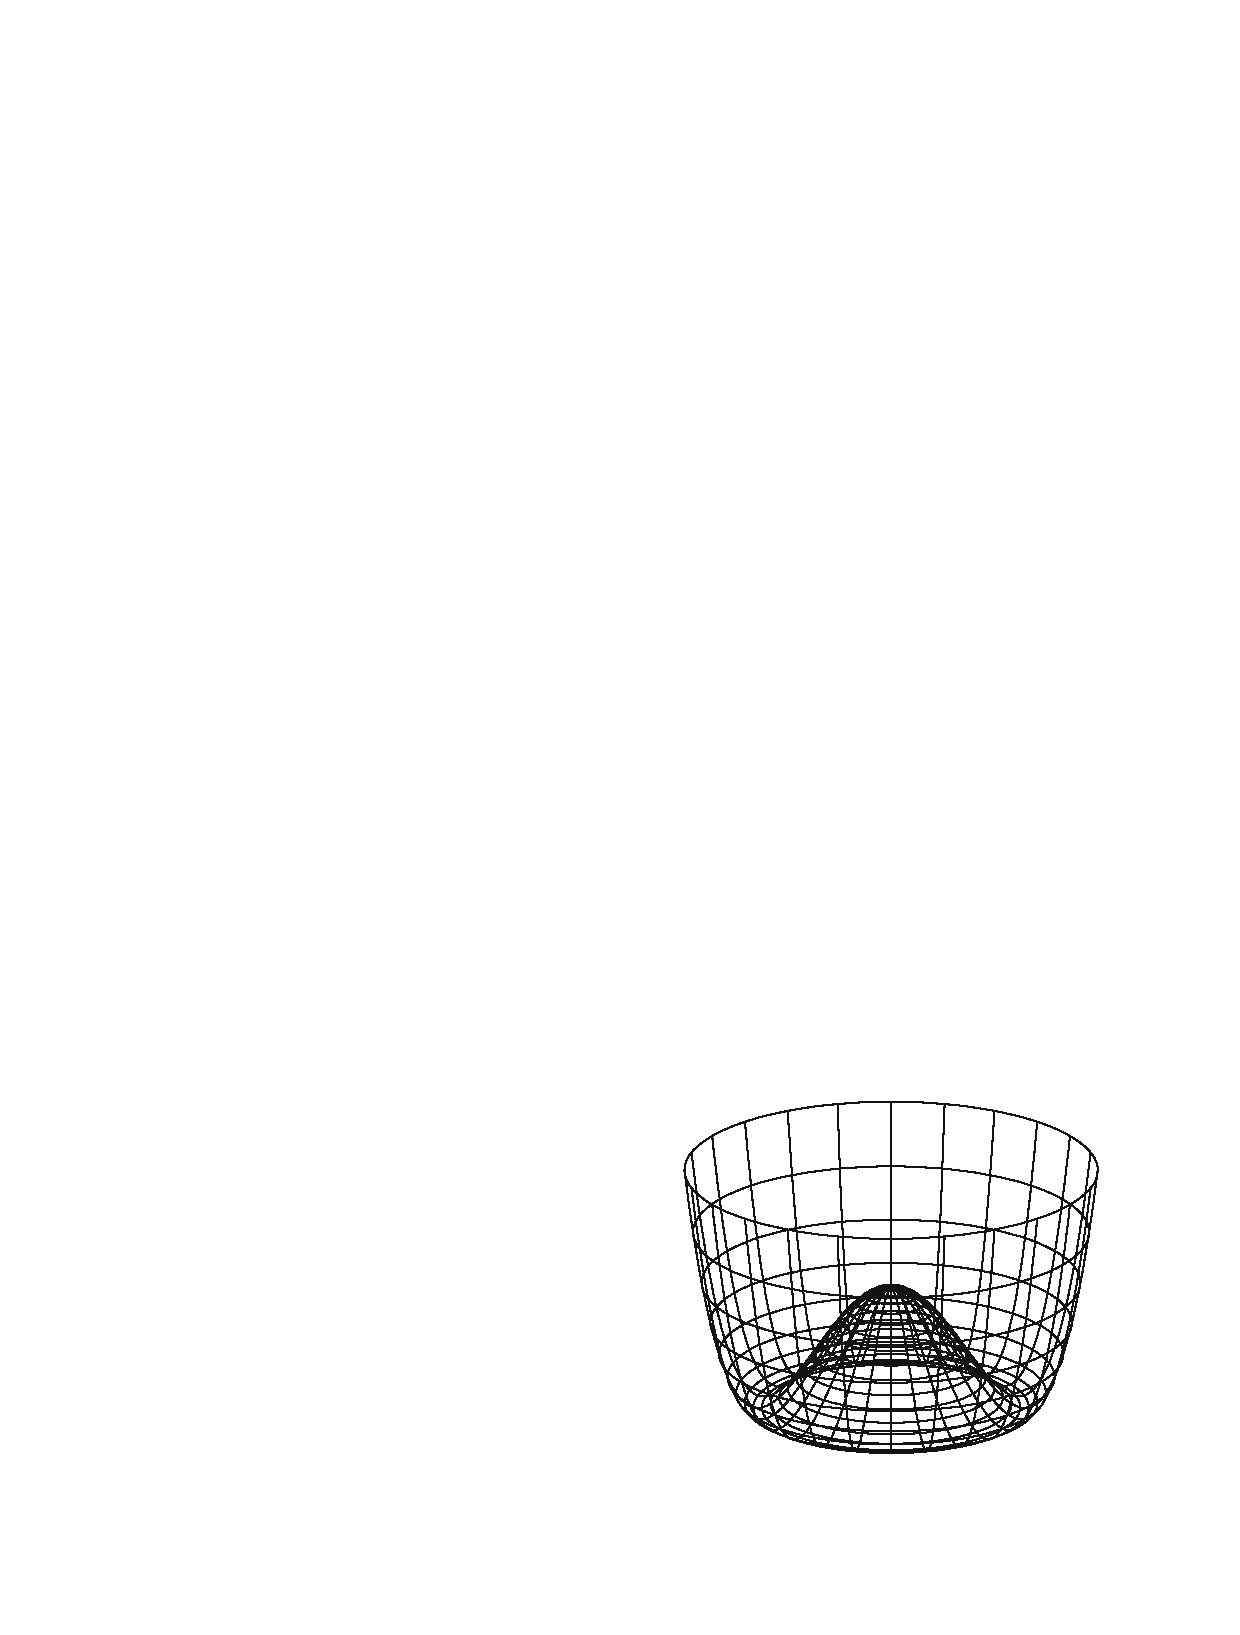
\includegraphics[width=0.5\textwidth]{Higgs_potential}
\caption[The Higgs field potential]{The Higgs field potential in the complex plane, commonly referred to as a
``Mexican hat'' potential \autocite{top_quark_at_HC}}
\label{fig:higgs_potential}
\end{figure}

The choice of minimum corresponding to the lowest energy state (or vacuum) is completely arbitrary. In fact, any point
at which the potential is minimum loses the invariance under $SU(2)_L \times U(1)_Y$ gauge transformations. Therefore,
nature spontaneously breaks the symmetry by picking the vacuum from the set of minima of the Higgs potential.
Conventionally, we can choose
\begin{equation}
\langle 0 | \phi | 0 \rangle = \frac{1}{\sqrt{2}} \twovector{0}{v}.
\label{eq:unitary_gauge_vev}
\end{equation}

Expanding around the chosen minimum, $\phi$ is then given by
\begin{equation}
\phi = \frac{1}{\sqrt{2}} \twovector{0}{v+H},
\end{equation}
where $H$ is the neutral scalar Higgs field. By substituting this field into the Lagrangian in
Equation~\ref{eq:Higgs_L}, one can obtain:
\begin{equation}
\begin{split}
\calL_\textrm{Higgs} & = \frac{1}{2} (\partial_\mu H)(\partial^\mu H) + \frac{1}{4} g^2 (H^2 + 2vH + v^2) W^+_\mu
W^{-\mu} + \\ & + \frac{1}{8} (g^2 + {g'}^2)(H^2 + 2vH + v^2)Z_\mu Z^\mu - \\ & - \mu^2 H^2 - \frac{\lambda}{4} (H^4 +
4vH^3),
\end{split}
\label{eq:Higgs_L_final}
\end{equation}
where physical fields $W^{\pm}_\mu$ and $Z_\mu$ are given by Equations~\ref{eq:W_mu} and \ref{eq:Z_mu}, respectively.
Notably, we can see that these fields have acquired mass terms in the Lagrangian, with the masses of vector bosons given
by
\begin{subequations}
\begin{align}
M_W &= \frac{1}{2}gv, \\
M_Z &= \frac{1}{2}v\sqrt{g^2+{g'}^2} = \frac{1}{2} \frac{gv}{\cos{\theta_W}},
\end{align}
\end{subequations}
whereas the mass of the Higgs boson itself is given by
\begin{equation}
M_H = \sqrt{2} \mu = v \sqrt{2\lambda}.
\end{equation}

% Unlike the \W and \Z boson masses which can be predicted from the measurement of the fine structure constant, the Higgs
% mass $M_H$ can not be determined by other experimentally measured parameters.

% However, it is possible to put indirect constraints on $M_H$ through quantum loop corrections and precise measurement of
% the \W boson and top quark masses. This will be discussed in Section~\ref{s:top_quak_physics}.

Naturally, the photon field $A_\mu$ acquires no mass terms in the Lagrangian. The Higgs mechanism can also be used in a
similar way to generate fermion masses by introducing an $SU(2)_L \times U(1)_Y$ gauge invariant term responsible for
interaction between the Higgs and fermion fields. This additional term in the Standard Model Lagrangian is called
\textit{Yukawa term}, which for the first generation of fermions is given by
\begin{equation}
\calL_\textrm{Yukawa} = -Y_e^{ij} \bar{l_L}^i \phi e_R^j - Y_u^{ij} \bar{q_L}^i \epsilon \phi^\dag u_R^j - Y_d^{ij}
\bar{q_L}^i \phi d_R^j + \textrm{h.c.},
\end{equation}
where coefficients $Y_{e,u,d}^{ij}$ are $3\times3$ complex matrices (Yukawa couplings) and $\epsilon$ is the $2\times2$
antisymmetric tensor. When the Higgs field $\phi$ acquires the vacuum expectation value given by
Equation~\ref{eq:unitary_gauge_vev}, the Yukawa Lagrangian yields mass terms for fermions, generating the masses:
\begin{equation}
M_f = Y_f \frac{v}{\sqrt{2}}.
\end{equation}

The Yukawa couplings are not diagonal in general, which results in mixing between different generations described for
the quarks by the CKM matrix (Equation~\ref{eq:CKM}). Another curious observation is that the fermion masses are
proportional to Yukawa couplings, which essentially represent the interaction strength with the Higgs field. Due to the
large mass of the top quark of approximately \SI{173}{\GeV}, and the Higgs field vacuum expectation value
$v\approx\SI{246}{\GeV}$, the Yukawa coupling to the top quark is very close to unity.

The existence of the Higgs boson and therefore the nature of electroweak symmetry breaking had long remained a mystery.
In the summer of 2012 both ATLAS and CMS experiments at the LHC observed the Higgs boson with an approximate mass of
\SI{125}{\GeV} \autocite{ATLAS_higgs_observation, CMS_higgs_observation}, with couplings consistent with theoretical
predictions \autocite{CMS_Higgs_long_paper, ATLAS_Higgs_couplings}, which proved to be yet another triumph of the
Standard Model.

\section{Shortcomings of the SM and physics beyond the SM}
\label{s:SM_shortcomings}
Despite being the most successful theory up to date, the Standard Model is not perfect and has its shortcomings. There
is a range of physical phenomena not explained by the SM. Let us mention the most prominent ones.

\begin{description}[wide=\parindent]
\item [Gravity] is not included in the Standard Model, as a consistent theory of quantum gravity is yet to be derived.
General relativity, the only accepted theory of gravity, is in fact fundamentally incompatible with quantum mechanics
and therefore the Standard Model.
\item [Massive neutrinos] are also not explained by the SM. The evidence for neutrino oscillations was confirmed by the
Super-Kamiokande collaboration \autocite{neutrino_oscillations}, which necessarily implies that neutrinos are massive
particles. It is possible to include massive neutrinos in some extensions of the Standard Model, whilst also keeping the
local symmetry of weak interactions \autocite{Shaposhnikov_nuMSM}. However, this leads to new theoretical problems
(e.g.\ unnaturally small neutrino Yukawa couplings).
\item [Matter/antimatter asymmetry,] which is apparent in the Universe, is not fully accounted for by the observed CP
violation in the Standard Model \autocite{Peskin_matter_antimatter, matter_antimatter_asymmetry}. Therefore, another
mechanism inducing the matter/antimatter asymmetry must exist, most likely requiring new physics models beyond the
Standard Model.

%\item [Strong CP problem] refers to the absence of any fundamental theoretical prohibition of CP violation in strong
%interactions. However, such strong CP violation has not been observed.
\item [Dark matter and dark energy] constitute approximately \SI{95}{\pc} of the mass/energy content in our Universe,
according to the latest Planck data \autocite{planck2013-p01, planck2013-p11}. The Standard Model only describes the
remaining \SI{5}{\pc} (i.e.\ ordinary matter), whereas the origin of dark matter and dark energy remains unknown.
\end{description}

Furthermore, there is a number of fundamental theoretical issues within the Standard Model, implying the intrinsic
incompleteness of the theory. The SM does not explain why it has only three generations of fermions. Moreover, there is
no explanation for the vast difference between masses of fermions (known as the Flavour problem), hence the origin of
Yukawa couplings (and therefore the CKM matrix) remains an open problem in particle physics.

Additionally, the \textit{ad hoc} nature of the Higgs mechanism gives rise to the hierarchy problem, which is related to
quadratic divergence of the loop corrections to the Higgs boson mass. The Higgs mass is renormalised by loop diagrams
(e.g.\ shown in Figure~\ref{fig:Higgs_loops}), making it extremely large  -- of the order of Planck scale (\SI{\sim
e19}{\GeV}) -- unless there is some unnatural fine tuning involved.

\begin{figure}[!hbtp]
	\centering
	\begin{minipage}[b]{0.4\textwidth}
	\centering
	\subfloat[]{
		\begin{fmfgraph*}(100,50)
		\fmfleft{i}
		\fmfright{o}
		\fmflabel{$H$}{i}
		\fmflabel{$H$}{o}
		\fmf{dashes,tension=3}{i,v1}
		\fmf{dashes,tension=3}{v2,o}
		\fmf{fermion,left,tension=1}{v1,v2,v1}
		\fmfdot{v1,v2}
		\end{fmfgraph*}
	}
	\end{minipage}
	\hspace{1cm}
	\begin{minipage}[b]{0.4\textwidth}
	\centering
	\subfloat[]{
		\begin{fmfgraph*}(100,50)
		\fmfleft{i}
		\fmfright{o}
		\fmflabel{$H$}{i}
		\fmflabel{$H$}{o}
		\fmf{dashes}{i,v1}
		\fmf{dashes}{v1,o}
		\fmffreeze
		\fmf{dashes,tension=1}{v1,v1}
		\fmfdot{v1}
		\end{fmfgraph*}
	}
	\end{minipage}
	\caption[Loop contributions to the Higgs boson mass]{Loop contributions to the Higgs boson mass: (a) fermion loops, (b)
	boson loops.}
  \label{fig:Higgs_loops}
\end{figure}


All these problems motivate the need for new models, referred to as physics beyond the Standard Model (BSM). Most
notable BSM models are briefly mentioned below.

\begin{description}[wide=\parindent]
\item [Supersymmetry] (SUSY) \autocite{SUSY_primer} is an extension of the SM, introducing a supersymmetric partner to
each ordinary particle by varying its spin by $1/2$. Thus, each fermion has a bosonic partner, and all bosons have
fermionic partners. Despite the greater number of free parameters, SUSY offers attractive solutions to most of the
mentioned problems of the SM. For example, the hierarchy problem is naturally solved in SUSY since the loop corrections
are automatically cancelled by corresponding contributions from supersymmetric partners. Most SUSY models also provide
good candidates for Dark Matter.
\item [Extra dimensions] refer to theories containing additional space-time dimensions, in which gravity is allowed to
propagate. This leads to reduction of the hierarchy between the Planck and electroweak scales, thus resolving the
hierarchy problem \autocite{Arkani-Hamed, RS}.
\item [Composite models,] such as topcolour \autocite{topcolour} or composite Higgs \autocite{composite_Higgs} models,
attempt to resolve some of the issues of the Standard Model by either introducing new composite particles or suggesting
a composite nature for the existing particles in the SM.
%\item [Grand Unified Theories (GUTs)] are a range of models striving to unify all fundamental forces.
\end{description}

An important and desirable feature of any physics model is its falsifiability in the accessible energy range. A wide
range of BSM models provide particle candidates that may exhibit themselves at the energy scale accessible at the LHC,
therefore a rich physics programme at the LHC must ensure an active search for all possible signs of new physics.

\newpage
\section{Top Quark Physics within the Standard Model}
\label{s:top_quak_physics}
The top quark is the heaviest elementary particle in the Standard Model, and the heaviest observed particle, discovered
in 1995 at the Tevatron collider by CDF and D{\O} collaborations \autocite{CDF_top_observation, D0_top_observation}. The
large mass of approximately \SI{173}{\GeV} suggests that the top quark may have a special role in nature. It is
substantially more massive than any other fermion. As mentioned in Section~\ref{s:SM_shortcomings}, the reason for such
vast discrepancy between fermion masses is not known. It is also not yet understood why the top quark's Yukawa coupling
to the Higgs boson is so close to unity. Naturally, studying the most massive fermion is a logical starting point in
search for answers to these questions.

Due to its large mass, the top quark has an extremely short lifetime of \SI{\approx5e-25}{\s} \autocite{PDG}, meaning
that it decays before the top-flavoured hadrons or \ttbar bound states can form. Therefore, the spin information is
passed from the top quark on to its decay products, providing a unique possibility to study a ``bare'' quark.
High-precision measurements of the top quark properties, such as mass (Chapter~\ref{c:top_mass_analysis}) and cross
section (Chapter~\ref{c:xsection_analysis}) are important tools to test the Standard Model and probe for new physics
beyond it.

\subsection{Top quark production at the LHC}
\label{ss:top_production}
There are two particular mechanisms of top quark production in hadron collisions: top-antitop (\ttbar) pair production
via the strong interaction, and single top quark production via the electroweak interaction. The \ttbar production
dominates over single top production, being the main source of top quarks at the LHC, and therefore is the main focus of
this thesis.

Feynman diagrams for \ttbar production to leading order are presented in
Figure~\ref{fig:ttbar_production_feynman_diagrams}. At the LHC, the major process for \ttbar production is gluon fusion,
constituting approximately \SI{90}{\pc} (\SI{80}{\pc}) at $\sqrt s =$ \SI{14}{\TeV} (\SI{7}{\TeV}) \autocite{PDG}.
Quark-antiquark annihilation and higher-order processes contribute the rest of the Standard Model \ttbar production.
This happens due to the fact that the LHC is a proton-proton collider, and the only source of antiquarks are virtual
quarks (so-called sea quarks). At the Tevatron, which was a proton-antiproton collider, the quark-antiquark annihilation
was the main \ttbar production mode.

\begin{figure}[!htbp]
	\begin{minipage}[t]{0.49\textwidth}
	\centering
	\subfloat[]{
		\begin{fmfgraph*}(150,75)
		\fmfleft{i1,i2}
		\fmfright{o1,o2}
		\fmflabel{$g$}{i1}
		\fmflabel{$g$}{i2}
		\fmflabel{$\bar{t}$}{o1}
		\fmflabel{$t$}{o2}

		\fmf{gluon}{i1,v1}
		\fmf{gluon}{i2,v2}
		\fmf{fermion}{v1,v2}
		\fmf{fermion}{o1,v1}
		\fmf{fermion}{v2,o2}
		\end{fmfgraph*}
	}
	\end{minipage}
	\hfill
	\begin{minipage}[t]{0.49\textwidth}
	\centering
	\subfloat[]{
		\begin{fmfgraph*}(150,75)
		\fmfleft{i1,i2}
		\fmfright{o1,o2}
		\fmflabel{$g$}{i1}
		\fmflabel{$g$}{i2}
		\fmflabel{$\bar{t}$}{o1}
		\fmflabel{$t$}{o2}

		\fmf{gluon}{i1,v1}
		\fmf{gluon}{i2,v1}
		\fmf{gluon}{v1,v2}
		\fmf{fermion}{o1,v2}
		\fmf{fermion}{v2,o2}
		\end{fmfgraph*}
	}
	\end{minipage}

	\vspace{1cm}

	\begin{minipage}[t]{0.49\textwidth}
	\centering
	\subfloat[]{
		\begin{fmfgraph*}(150,75)
		\fmfleft{i1,i2}
		\fmfright{o1,o2}
		\fmflabel{$g$}{i1}
		\fmflabel{$g$}{i2}
		\fmflabel{$\bar{t}$}{o1}
		\fmflabel{$t$}{o2}

		\fmf{gluon}{i1,v1}
		\fmf{phantom}{v1,o1}
		\fmf{gluon}{i2,v2}
		\fmf{phantom}{v2,o2}
		\fmf{fermion}{v2,v1}

		\fmf{fermion,tension=0}{v1,o2}
		\fmf{fermion,tension=0}{o1,v2}

		\end{fmfgraph*}
	}
	\end{minipage}
	\hfill
	\begin{minipage}[t]{0.49\textwidth}
	\centering
	\subfloat[]{
		\begin{fmfgraph*}(150,75)
		\fmfleft{i1,i2}
		\fmfright{o1,o2}
		\fmflabel{$\bar{q}$}{i1}
		\fmflabel{$q$}{i2}
		\fmflabel{$\bar{t}$}{o1}
		\fmflabel{$t$}{o2}

		\fmf{fermion}{v1,i1}
		\fmf{fermion}{i2,v1}
		\fmf{gluon}{v1,v2}
		\fmf{fermion}{o1,v2}
		\fmf{fermion}{v2,o2}
		\end{fmfgraph*}
	}
	\end{minipage}

	\caption[Feynman diagrams for leading order \ttbar production at the LHC]{Feynman diagrams for leading order \ttbar
	production at the LHC: (a), (b) and (c) show the gluon fusion, the dominant production mechanism, (d) represents
	quark-antiquark annihilation.}
  \label{fig:ttbar_production_feynman_diagrams}
\end{figure}

Figure~\ref{fig:single_top_production_feynman_diagrams} shows the Feynman diagrams of various single top production
modes. Three major production mechanisms include s-channel and t-channel \W boson exchange, and associated production
with a \W boson (tW-channel). Measurement of single top production is of significant interest since it allows the direct
measurement of the Wtb vertex and therefore the magnitude of $|V_{tb}|$ element of the CKM matrix.

\begin{figure}[!hbtp]
	\centering
	\vspace*{0.5cm}
	\begin{minipage}[b]{0.3\textwidth}
	\centering
	\subfloat[]{
		\begin{fmfgraph*}(150,75)
		\fmfleft{i1,i2}
		\fmfright{o1,o2}
		\fmflabel{$q$}{i1}
		\fmflabel{$\bar{q}'$}{i2}
		\fmflabel{$\bar{b}$}{o1}
		\fmflabel{$t$}{o2}

		\fmf{fermion}{i1,v1}
		\fmf{fermion}{v1,i2}
		\fmf{photon, label=$W$}{v1,v2}
		\fmf{fermion}{o1,v2}
		\fmf{fermion}{v2,o2}
		\end{fmfgraph*}
	}
	\end{minipage}
	\hfill
	\begin{minipage}[b]{0.3\textwidth}
	\centering
	\subfloat[]{
		\begin{fmfgraph*}(150,75)
		\fmfleft{i1,i2}
		\fmfright{o1,o2,o3}
		\fmflabel{$g$}{i1}
		\fmflabel{$q$}{i2}
		\fmflabel{$\bar{b}$}{o1}
		\fmflabel{$t$}{o2}
		\fmflabel{$q'$}{o3}

		\fmf{gluon}{i1,v1}
		\fmf{fermion}{i2,v3}
		\fmf{fermion, label=$b$}{v1,v2}
		\fmf{photon, label=$W$}{v2,v3}
		\fmf{fermion}{o1,v1}
		\fmf{fermion}{v2,o2}
		\fmf{fermion}{v3,o3}
		\end{fmfgraph*}
	}
	\end{minipage}
	\hfill
	\begin{minipage}[b]{0.3\textwidth}
	\centering
	\subfloat[]{
		\begin{fmfgraph*}(150,75)
		\fmfleft{i1,i2}
		\fmfright{o1,o2}
		\fmflabel{$b$}{i1}
		\fmflabel{$q$}{i2}
		\fmflabel{$t$}{o1}
		\fmflabel{$q'$}{o2}

		\fmf{fermion}{i1,v1}
		\fmf{fermion}{i2,v2}
		\fmf{photon, label=$W$}{v1,v2}
		\fmf{fermion}{v1,o1}
		\fmf{fermion}{v2,o2}
		\end{fmfgraph*}
	}
	\end{minipage}

	\vspace{1cm}

	\hfill

	\begin{minipage}[t]{0.3\textwidth}
	\centering
	\subfloat[]{
		\begin{fmfgraph*}(150,75)
		\fmfleft{i1,i2}
		\fmfright{o1,o2}
		\fmflabel{$g$}{i1}
		\fmflabel{$b$}{i2}
		\fmflabel{$t$}{o1}
		\fmflabel{$W$}{o2}

		\fmf{gluon}{i1,v1}
		\fmf{fermion}{i2,v1}
		\fmf{fermion, label=$b$}{v1,v2}
		\fmf{fermion}{v2,o1}
		\fmf{photon}{v2,o2}
		\end{fmfgraph*}
	}
	\end{minipage}
	\hspace{2cm}
	\begin{minipage}[t]{0.3\textwidth}
	\centering
	\subfloat[]{
		\begin{fmfgraph*}(150,75)
		\fmfleft{i1,i2}
		\fmfright{o1,o2}
		\fmflabel{$b$}{i1}
		\fmflabel{$g$}{i2}
		\fmflabel{$W$}{o1}
		\fmflabel{$t$}{o2}

		\fmf{fermion}{i1,v1}
		\fmf{gluon}{i2,v2}
		\fmf{fermion, label=$t$}{v1,v2}
		\fmf{photon}{v1,o1}
		\fmf{fermion}{v2,o2}
		\end{fmfgraph*}
	}
	\end{minipage}
	\hfill

	\caption[Feynman diagrams for leading order single top production]{Feynman diagrams for leading order
	single top production. (a) s-channel, (b) and (c) t-channel, (d) and (e) tW-channel.}
  \label{fig:single_top_production_feynman_diagrams}
\end{figure}

\subsection{Top quark decay}
\label{ss:top_decay}
The top quark predominantly decays to a \W boson and a b-quark: $\cPqt \rightarrow \W \cPqb$. Other possible decay modes
($\cPqt \rightarrow \W \cPqs$ and $\cPqt \rightarrow \W \cPqd$) are suppressed in the Standard Model by the unitarity
requirement of the CKM matrix, which yields \autocite{PDG} the $|V_{tb}|$ value of
\begin{equation}
|V_{tb}| = 0.999146^{+0.000021}_{-0.000046}.
\end{equation}

As it was previously mentioned, the direct measurement of $|V_{tb}|$ (without assuming unitarity) can be performed by
measuring the single top production cross section. The recent CMS result is consistent with the Standard
Model \autocite{single_top_Vtb_CMS}:
\begin{equation}
|V_{tb}| = 0.998 \pm 0.038~\textrm{(experimental)} \pm 0.016~\textrm{(theoretical)}.
\end{equation}

The branching fraction of $\cPqt \rightarrow \W \cPqb$ decay is assumed to be \SI{100}{\pc} hereafter. Therefore, the
\ttbar decay modes completely depend on subsequent \W boson decays:
\begin{itemize}
  \item fully hadronic: \ttbar $\rightarrow \cPqb \W^+ ~ \bar{\cPqb} \W^- \rightarrow  \cPqb~\cPq\bar{\cPq}' ~
  \bar{\cPqb}~\cPq'' \bar{\cPq}'''$ (\SI{45.7}{\pc});
  \item semileptonic: \ttbar $\rightarrow \cPqb \W^+ ~ \bar{\cPqb} \W^- \rightarrow \cPqb~\cPq\bar{\cPq}' ~ \bar{\cPqb}
  ~ l^- \bar{\nu}_l + \cPqb~l^+ \nu_l ~ \bar{\cPqb}~\cPq'' \bar{\cPq}'''$ (\SI{43.8}{\pc});
  \item dileptonic: \ttbar $\rightarrow \cPqb \W^+ ~ \bar{\cPqb} \W^- \rightarrow  \cPqb~\bar{l} \nu_l ~ \bar{\cPqb} ~
  l'\bar{\nu}_{l'}$ (\SI{10.5}{\pc}).
\end{itemize}

Percentages in parentheses show the branching fractions corresponding to the decay modes \autocite{PDG}. The quarks in
all final states hadronise into jets. The number of jets is not limited to the number of initial quarks due to the
contribution from extra QCD radiation (i.e.\ gluon radiation) either before or after \ttbar production.

The fully hadronic \ttbar decay signature implies at least 6 jets in the final state and no leptons, hence it is heavily
contaminated by the background from QCD and \W/\ZpJets processes. Dileptonic \ttbar decay has a clean signature, but due
to the lowest branching fraction can suffer from limited statistics. The semileptonic decay mode, shown in
Figure~\ref{fig:ttbar_semileptonic_decay}, has exactly one highly energetic lepton and at least four jets in the final
state, which is therefore called the lepton plus jets final state. The lepton can be an electron, a muon or a
$\tau$-lepton; however, since the $\tau$-leptons are difficult to reconstruct, they are usually excluded from top quark
analyses studying semileptonic decays. Analyses in this thesis study the electron plus jets ($e+$jets) and muon plus
jets ($\mu+$jets) decay channels, which have branching fractions of \SI{\approx14}{\pc} each.

\begin{figure}[!hbtp]
	\centering
	\vspace*{0.5cm}
	\begin{fmfgraph*}(300,150)
	\fmfleft{i1,i2,i3}
	\fmfright{o1,o2,o3}
	\fmflabel{$\bar{q}$}{i1}
	\fmflabel{$q$}{i2}
	\fmflabel{$\bar{b}$}{i3}
	\fmflabel{$b$}{o1}
	\fmflabel{$l^+$}{o2}
	\fmflabel{$\nu_l$}{o3}
	
	\fmf{fermion}{i3,v2}
	\fmf{phantom}{i1,v2}
	\fmf{fermion, label=$\bar{t}$}{v2,v3}
	\fmf{fermion, label=$t$}{v3,v4}
	\fmf{fermion}{v4,o1}
	\fmf{phantom}{o3,v4}
	\fmffreeze
	\fmf{fermion}{i1,v1}
	\fmf{fermion}{v1,i2}
	\fmf{fermion}{o2,v5}
	\fmf{fermion}{v5,o3}
	\fmf{photon, label=$W^-$}{v1,v2}
	\fmf{photon, label=$W^+$}{v4,v5}
	\fmfdot{v3}
	\end{fmfgraph*}
	\caption{Semileptonic \ttbar decay mode}
  \label{fig:ttbar_semileptonic_decay}
\end{figure}


\newpage
\subsection{Background processes to semileptonic top quark pair decay}
\label{ss:backgrounds}
Both top quark mass and differential cross section analyses presented in this thesis are based on selection of events
with semileptonic ($e/\mu+$jets) \ttbar decay signature. Being relatively clean yet still providing sufficient event
yields, this decay mode is used in many measurements of top quark properties, and is often called a ``golden channel''
in top quark physics. Good understanding of background contributions is very important for accuracy and reliability of
measurements. The most significant background processes to semileptonic \ttbar decay are described below.

\subsubsection*{Single top quark background}
One of the less significant backgrounds to lepton plus jets analyses is the single top quark production. Major
production modes for this process (mentioned in Section~\ref{ss:top_production}) have a lower number of jets in the
final state than that of the \ttbar production, however, additional jets can emerge from inital and final state
radiation (ISR/FSR), i.e.\ soft gluon radiation before and after the hard scattering process. This contribution is not
negligible, and is modelled using Monte Carlo simulation.

\subsubsection*{\WpJets background}
Production of \W bosons with additional jets (called \WpJets) is one of the most significant backgrounds to semileptonic
\ttbar decays. Example Feynman diagrams for leading order \W boson production are shown in
Figure~\ref{fig:VJets_processes} (a, b). Leptonic decays in the \WpJets process together with extra jets can
successfully mimic the \ttbar decay since it also includes two \W bosons. However, leptons and jets in \WpJets processes
are usually much softer than those coming from \ttbar decay, due to the large mass of top quarks. Moreover, additional
jets are less likely to be \cPqb-jets which are necessarily present in \ttbar decay. Therefore, tagging of \cPqb-jets
and high kinematic cuts on lepton and jets transverse momenta can significantly reduce the
\WpJets background. Besides, the production cross section of \WpJets events reduces exponentially with increasing number
of jets \autocite{multijet_WZ}, therefore jet multiplicity cuts also help to mitigate this background. These methods are
detailed in selection procedures of top quark mass and differential cross section analyses in
Sections~\ref{s_top_mass:event_selection} and \ref{s_xsection:event_selection}, respectively.

\subsubsection*{\ZpJets background}
\Z boson production processes with additional jets (\ZpJets) are largely similar to \WpJets processes, as can be seen in
Figure~\ref{fig:VJets_processes} (c, d). The difference lies in leptonic decays of the \Z boson, as it produces two
opposite-sign leptons. Vetoing the second lepton in the selection is therefore particularly helpful in reducing this
background. Contamination can still occur if one of the leptons is misreconstructed as a jet or does not pass
identification criteria. This contribution is estimated to be small, and together with the jet multiplicity cuts the
\ZpJets background is usually mitigated significantly.

\begin{figure}[tbp]
	\begin{minipage}[t]{0.49\textwidth}
	\centering
	\subfloat[]{
		\begin{fmfgraph*}(150,75)
		\fmfleft{i1,i2}
		\fmfright{o1,o2}
		\fmflabel{$q$}{i1}
		\fmflabel{$g$}{i2}
		\fmflabel{$q'$}{o1}
		\fmflabel{$W$}{o2}

		\fmf{fermion}{i1,v1}
		\fmf{gluon}{i2,v1}
		\fmf{fermion}{v1,v2}
		\fmf{fermion}{v2,o1}
		\fmf{photon}{v2,o2}
		\end{fmfgraph*}
	}
	\end{minipage}
	\hfill
	\begin{minipage}[t]{0.49\textwidth}
	\centering
	\subfloat[]{
		\begin{fmfgraph*}(150,75)
		\fmfleft{i1,i2}
		\fmfright{o1,o2}
		\fmflabel{$q$}{i1}
		\fmflabel{$\bar{q}'$}{i2}
		\fmflabel{$g$}{o1}
		\fmflabel{$W$}{o2}

		\fmf{fermion}{i1,v1}
		\fmf{fermion}{v2,i2}
		\fmf{fermion}{v1,v2}
		\fmf{gluon}{v1,o1}
		\fmf{photon}{v2,o2}
		\end{fmfgraph*}
	}
	\end{minipage}

	\vspace{1cm}

	\begin{minipage}[t]{0.49\textwidth}
	\centering
		\subfloat[]{
		\begin{fmfgraph*}(150,75)
		\fmfleft{i1,i2}
		\fmfright{o1,o2}
		\fmflabel{$q$}{i1}
		\fmflabel{$g$}{i2}
		\fmflabel{$q'$}{o1}
		\fmflabel{$Z$}{o2}

		\fmf{fermion}{i1,v1}
		\fmf{gluon}{i2,v1}
		\fmf{fermion}{v1,v2}
		\fmf{fermion}{v2,o1}
		\fmf{photon}{v2,o2}
		\end{fmfgraph*}
	}
	\end{minipage}
	\hfill
	\begin{minipage}[t]{0.49\textwidth}
	\centering
	\subfloat[]{
		\begin{fmfgraph*}(150,75)
		\fmfleft{i1,i2}
		\fmfright{o1,o2}
		\fmflabel{$g$}{i1}
		\fmflabel{$q$}{i2}
		\fmflabel{$q'$}{o1}
		\fmflabel{$Z$}{o2}

		\fmf{gluon}{i1,v1}
		\fmf{fermion}{i2,v2}
		\fmf{fermion}{v2,v1}
		\fmf{fermion}{v1,o1}
		\fmf{photon}{v2,o2}
		\end{fmfgraph*}
	}
	\end{minipage}

	\caption[Example diagrams for leading order \W and \Z boson production at the
	LHC.]{Example diagrams for leading order \W boson (a, b) and \Z boson (c,
	d) production at the LHC.}
  \label{fig:VJets_processes}
\end{figure}

\subsubsection*{QCD multi-jet background}
Standard QCD processes in hadron collisions, such as gluon fusion and quark-antiquark annihilation, usually result in
production of highly energetic jets. Examples of these processes in the lowest order with two jets in the final state
are shown in Figure~\ref{fig:QCD_processes}. Additional jets arise at higher orders and can potentially fake \ttbar
signal. Although QCD events do not produce real prompt leptons, this can happen when jets are mis-identified as leptons.
These objects are referred to as fake leptons. Due to strict identification criteria of real electrons and muons
(described in Sections~\ref{ss:electron_reconstruction} and \ref{ss:muon_reconstruction}), such mis-identifications are
extremely rare. However, since the production cross section of QCD events is very large, this background becomes
considerable.

\begin{figure}[tbp]
	\begin{minipage}[t]{0.49\textwidth}
	\centering
	\subfloat[]{
		\begin{fmfgraph*}(150,75)
		\fmfleft{i1,i2}
		\fmfright{o1,o2}
		\fmflabel{$q$}{i1}
		\fmflabel{$g$}{i2}
		\fmflabel{$\bar{q}$}{o1}
		\fmflabel{$q$}{o2}

		\fmf{gluon}{i1,v1}
		\fmf{gluon}{i2,v1}
		\fmf{gluon}{v1,v2}
		\fmf{fermion}{o1,v2}
		\fmf{fermion}{v2,o2}
		\end{fmfgraph*}
	}
	\end{minipage}
	\hfill
	\begin{minipage}[t]{0.49\textwidth}
	\centering
	\subfloat[]{
		\begin{fmfgraph*}(150,75)
		\fmfleft{i1,i2}
		\fmfright{o1,o2}
		\fmflabel{$q$}{i1}
		\fmflabel{$g$}{i2}
		\fmflabel{$g$}{o1}
		\fmflabel{$g$}{o2}

		\fmf{gluon}{i1,v1}
		\fmf{gluon}{i2,v1}
		\fmf{gluon}{v1,v2}
		\fmf{gluon}{o1,v2}
		\fmf{gluon}{v2,o2}
		\end{fmfgraph*}
	}
	\end{minipage}

	\vspace{1cm}

	\begin{minipage}[t]{0.49\textwidth}
	\centering
		\subfloat[]{
		\begin{fmfgraph*}(150,75)
		\fmfleft{i1,i2}
		\fmfright{o1,o2}
		\fmflabel{$q$}{i1}
		\fmflabel{$g$}{i2}
		\fmflabel{$g$}{o1}
		\fmflabel{$q$}{o2}

		\fmf{fermion}{i1,v1}
		\fmf{gluon}{i2,v1}
		\fmf{fermion}{v1,v2}
		\fmf{gluon}{v2,o1}
		\fmf{fermion}{v2,o2}
		\end{fmfgraph*}
	}
	\end{minipage}
	\hfill
	\begin{minipage}[t]{0.49\textwidth}
	\centering
	\subfloat[]{
		\begin{fmfgraph*}(150,75)
		\fmfleft{i1,i2}
		\fmfright{o1,o2}
		\fmflabel{$q'$}{i1}
		\fmflabel{$q$}{i2}
		\fmflabel{$q'$}{o1}
		\fmflabel{$q$}{o2}

		\fmf{fermion}{i1,v1}
		\fmf{fermion}{i2,v2}
		\fmf{gluon}{v2,v1}
		\fmf{fermion}{v1,o1}
		\fmf{fermion}{v2,o2}
		\end{fmfgraph*}
	}
	\end{minipage}

	\caption[Example diagrams for leading order QCD multi-jet production at
	the LHC.]{Example diagrams for leading order QCD multi-jet production at
	the LHC.}
  \label{fig:QCD_processes}
\end{figure}

QCD multi-jet background is usually less significant in the muon plus jets channel, since jets faking muons are easier
to recognise. For instance, when a highly energetic jet punches through the calorimetry system into muon chambers and
thus becomes a fake muon, it can be removed by isolation criteria as it also leaves a significant energy deposit in
calorimeters. Muons (and electrons) can also arise from heavy flavour decays of \cPqb and \cPqc quarks -- these are in
fact real leptons, but as they don't originate at the interaction point, they can be removed by track quality cuts most
of the time.

In the electron plus jets channel, QCD multi-jet background is more prominent. This happens mainly due to photon
conversions, which occur when photons convert into electron-positron pairs. Photons can arise from prompt production
($\gamma+$jets), particle decays or bremsstrahlung radiation. Different methods of identifying such conversions have
been developed, which is discussed in detail in Section~\ref{sss:photon_conversions}.

Due to the large contribution from higher-order processes in signal region, the QCD background is very hard to model.
Large uncertainties in theoretical cross section and potential mismodelling of higher-order effects may lead to biases
in kinematic distributions based on Monte Carlo simulation, as well as in overall acceptance of QCD events passing the
signal selection. Therefore, data-driven methods of QCD background estimation are often preferable (see
Section~\ref{s_xsection:data_driven_QCD}).

\subsubsection*{Additional backgrounds}
Other background processes potentially mimicking semileptonic \ttbar decay include the Drell-Yan process with dilepton
production ($q \bar{q} \rightarrow \Z/\gamma^* \rightarrow l \bar{l}$), and diboson production. The background
contamination from these processes can be reduced by vetoing the second lepton, and is generally considered negligible
due to relatively small production cross sections of these processes.


\subsection{Top quark mass}
\label{ss:top_mass}
The top quark mass is a fundamental parameter of the Standard Model. However, its precise definition is a very
non-trivial problem, ultimately subject to convention. One of the most popular definitions is the pole mass,
corresponding to the real part of a pole in the perturbative propagator of a particle
\autocite{pole_mass_in_QCD_Tarrach}. For the top quark, the perturbative propagator with a four-momentum $p$ has a pole
at \autocite{top_pole_mass}:
\begin{equation}
\sqrt{p^2} = \mtop - \frac{i}{2} \Gamma_\textrm{t},
\end{equation}
where \mtop is the pole mass and $\Gamma_\textrm{t}~\SI{\approx1.5}{\GeV}$ is the top quark decay width. This definition
yields a peak in the invariant mass distribution of the top quark decay products (i.e.\ \W boson and \cPqb-quark), which
is accessible experimentally. As $\mtop \gg \Gamma_\textrm{t}/2$, the peak approximately corresponds to the pole mass,
therefore it is usually assumed that experimentally measured top quark mass represents the pole mass. As will be
discussed later, there are a few problems with this approach.

It has been shown \autocite{pole_mass_in_QCD_Kronfeld} that the pole mass is infrared finite and gauge-invariant to all
orders of perturbative QCD. Despite being well-defined in perturbation theory, an all-order resummation of a particular
class of diagrams known as ``infrared renormalons'' \autocite{renormalons1, renormalons2} leads to an intrinsic
ambiguity of the top quark pole mass proportional to the energy scale of a strong interaction
$\Lambda_\textrm{QCD}~\SI{\approx200}{\MeV}$
\autocite{pole_MS_top_difference}.

Another frequently used mass definition which is free from renormalon ambiguity is the renormalised mass $\MSmtop(\mu)$
in the minimal subtraction (\MS) renormalisation scheme. This mass definition is often call a running mass, since it
depends on the renormalisation scale $\mu$ which is in principle arbitrary. For a choice of $\mu=\MSmtop$, the \MS mass
\MSmtop is related to the pole mass \mtop as follows
\autocite{top_pole_mass}:
\begin{equation}
\mtop = \MSmtop(\MSmtop) \left( 1 + \frac{4}{3} \frac{\overline{\alpha}_S(\MSmtop)}{\pi} + 8.28
\left(\frac{\overline{\alpha}_S(\MSmtop)}{\pi} \right)^2 + ... \right) + \bigO(\Lambda_\textrm{QCD}).
\end{equation}
% \footnote{Renormalisation is a technique of cancelling divergences (infinities) in perturbative quantum field theories.
% Initially infinite parameters become finite after renormalisation, thus acquiring physical sense.}

The difference between the pole mass and the \MS mass is then estimated to be on the order of \SI{10}{\GeV} (with $\mtop
> \MSmtop$). However, it has recently been shown \autocite{pole_MS_top_difference} that including electroweak
corrections for a Higgs boson mass of \SI{\sim125}{\GeV} mostly cancels the corresponding QCD corrections, reducing the
$\mtop-\MSmtop$ difference down to \SI{\sim1}{\GeV}. Theoretical research such as studying higher-order corrections is
actively ongoing in this field.

It has been argued that the top quark mass measured at hadron colliders is in fact a parameter of Monte Carlo
generators, which does not necessarily correspond to the pole mass. This parameter is determined by (next to) leading
order calculations of the matrix elements of hard processes (see Section~\ref{s:MC_simulation}), and this mass
definition does not absorb any corrections from parton showers and hadronisation. Therefore, the actual mass definition
measured experimentally remains not fully understood, with a conceptual uncertainty on the order of
\SI{1}{\GeV} \autocite{measured_top_mass_interpretation}.

Nevertheless, experimental measurements of the top quark mass are of paramount importance. Continuously increasing
precision of the measurements is challenging the current definition of the measured mass, undoubtedly triggering more
effort in reaching a more precise theoretical specification of the mass parameter used in Monte Carlo simulation. As the
top quark is a major background to many new physics searches beyond the Standard Model, deep understanding of its mass
parameter in simulation as well as pushing down the corresponding theoretical and experimental uncertainties are
extremely important.

Nearly 20 years of the Tevatron operation resulted in a very good understanding of the machine and detectors, leading to
an impressively small systematic uncertainty on the top quark mass measurement. The latest combination result from the
Tevatron gives \autocite{tevatron_top_mass_combination}:
\begin{equation}
\mtop = 173.20 \pm 0.51~\textrm{(stat.)} \pm 0.71~\textrm{(syst.)}~\textrm{GeV}.
\end{equation}

The LHC experiments have reached nearly as good precision, with a statistical uncertainty being expectedly smaller
than that of the Tevatron, however, with a larger systematic error due still improving understanding of detector
effects. The latest LHC combination result yields \autocite{LHC_top_mass_combination}:
\begin{equation}
\mtop = 173.29 \pm 0.23~\textrm{(stat.)} \pm 0.92~\textrm{(syst.)}~\textrm{GeV}.
\end{equation}

Recently, the first world combination result of both LHC and Tevatron measurements has become available
\autocite{world_top_mass_combination}:
\begin{equation}
\mtop = 173.34 \pm 0.27~\textrm{(stat.)} \pm 0.71~\textrm{(syst.)}~\textrm{GeV},
\end{equation}
which corresponds to a total uncertainty on the top quark mass of \SI{0.76}{\GeV}, or \SI{0.44}{\pc}. All these results
compared with contributions of individual mass measurements are shown in Figure~\ref{fig:top_mass_world_combination}.

At a proposed linear electron-positron collider (International Linear Collider, ILC), the uncertainty on the top quark
mass is expected to fall below \SI{200}{\MeV}, i.e.\ the energy scale of the strong interaction $\Lambda_\textrm{QCD}$.
It will clearly challenge the theoretical understanding of different mass schemes, ultimately leading to more vigorous
tests of the Standard Model and potentially providing sensitivity to new physics models.

\begin{figure}[hbtp]
   \centering
   {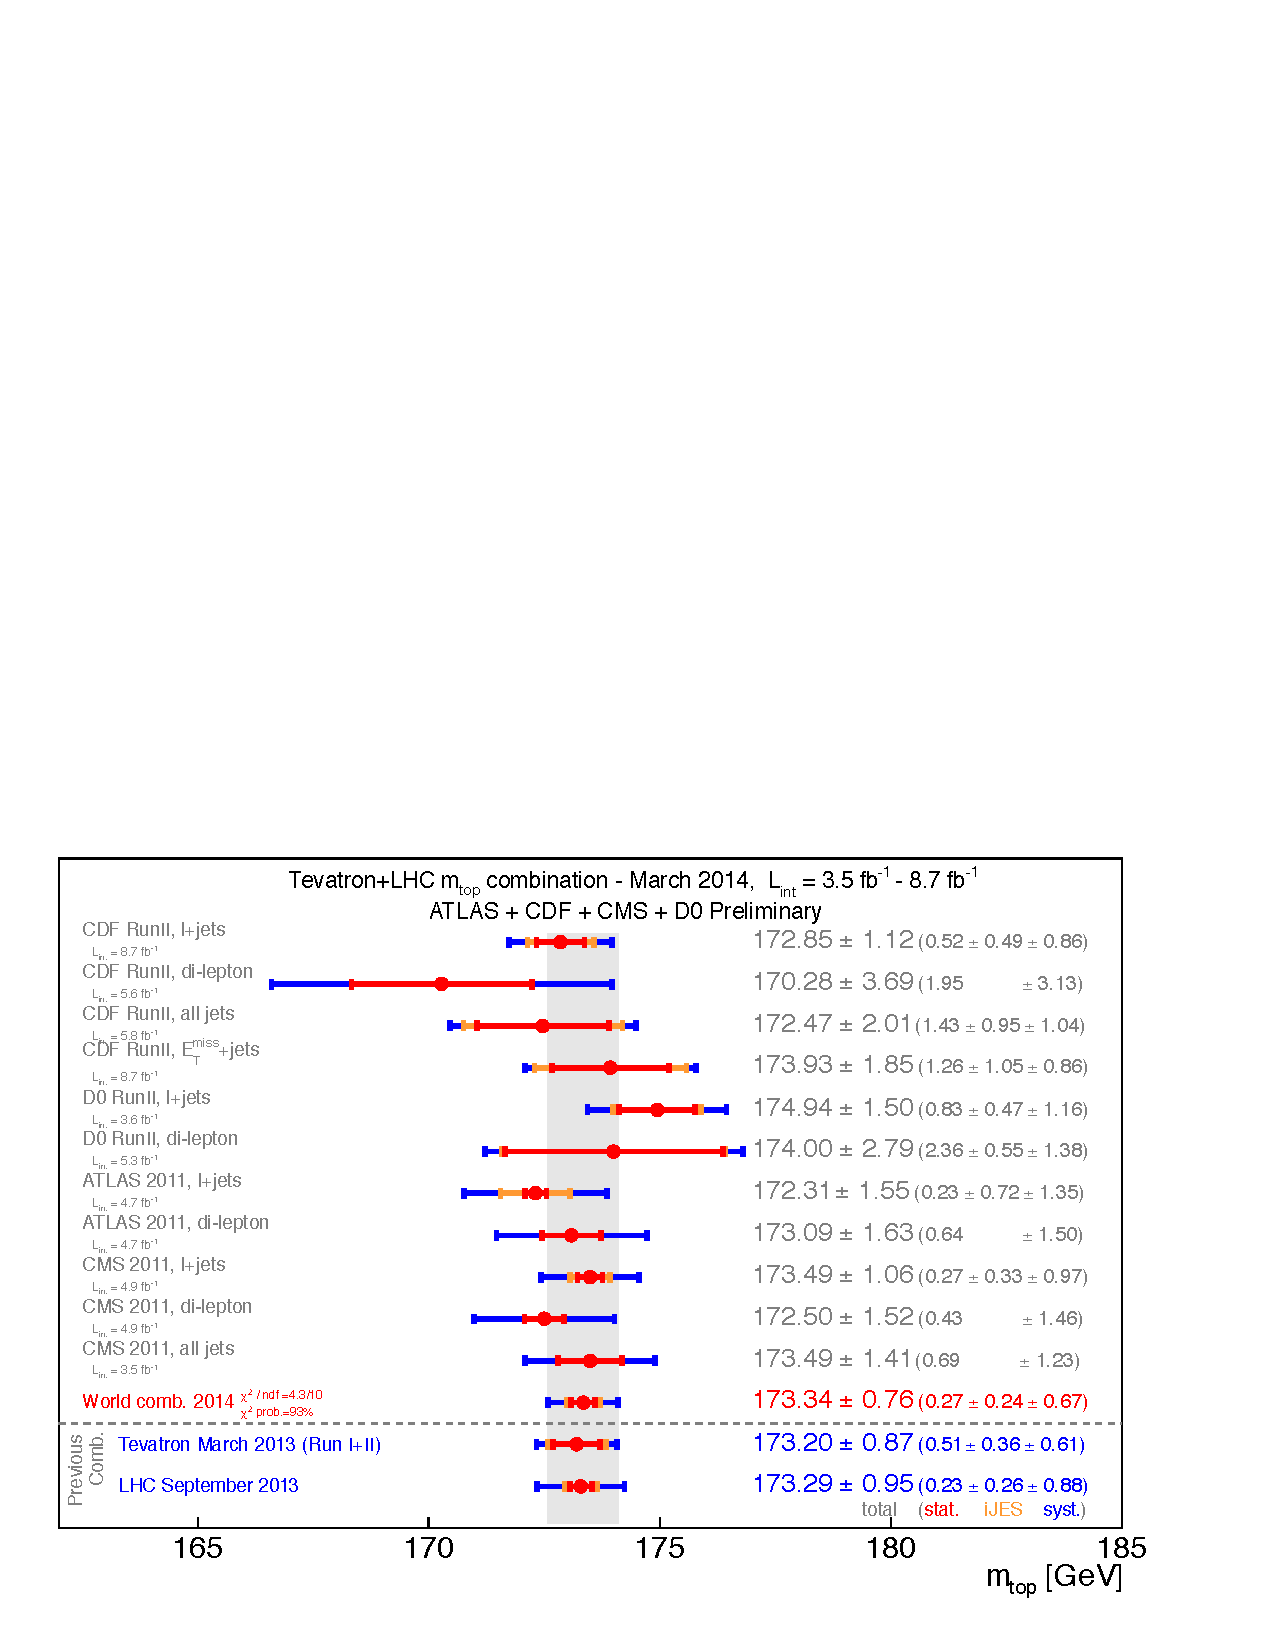
\includegraphics[width=0.9\textwidth]{top_world_combination}}
   \caption[World combination of the top quark mass measurements.]{Top quark mass measurements and the result of their
   combination, compared with the Tevatron and LHC combinations. Each measurement is shown with the total uncertainty,
   the statistical, the jet energy scale (iJES, when applicable), and the systematic uncertainty. The iJES contribution
   is statistical in nature and applies only to analyses performing \textit{in situ} jet energy calibration procedures.
   The grey vertical band shows the total uncertainty on the combined value of the top quark mass
   \autocite{world_top_mass_combination}.}
   \label{fig:top_mass_world_combination}
\end{figure}

\subsection{Top quark pair production cross section}
\label{ss:ttbar_cross_section}
The \ttbar production is a strong interaction process, and therefore is described by perturbative QCD. Hadron collisions
at the LHC (or other hadron colliders) are best viewed as interactions between their constituent quarks and gluons, also
referred to as partons. Since collisions occur at high energies, these interactions result in hard scattering processes
between incoming partons, meaning those involving a significant momentum transfer comparing to the proton mass, and
potentially giving rise to highly energetic final states like top quarks. Each incoming parton carries only a fraction
$x$ of the total momentum of a parent hadron. The distribution of momentum fractions for all flavours of partons are
described by parton distribution functions (PDFs).

A PDF $f_i(x_i,\mu_f^2)$ is defined as a probability density of finding a parton with flavour $i$ and a longitudinal
momentum fraction $x_i$ when probed at momentum scale $\mu_f^2$, which is known as factorisation scale. This parameter
separates the hard scattering process into the hard partonic interaction and the soft (or long-range) interaction. The
former interaction happens at a short distance, and therefore only involves high-momentum transfer which is calculable
in perturbative QCD. The soft long-range part of the interaction, on the contrary, can not be calculated in QCD and
instead is parametrised by the PDFs, which have to be obtained from experimental data. Figure~\ref{fig:CT10_PDFs} shows
one of the latest PDFs obtained by the CTEQ-TEA collaboration \autocite{CT10_NNLO}.

\begin{figure}[hbtp]
   \centering
   \subfloat[]{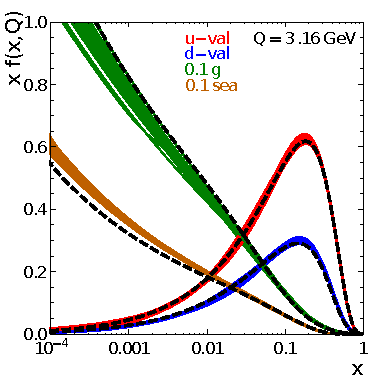
\includegraphics[width=0.5\textwidth]{CT10_1}}
   \subfloat[]{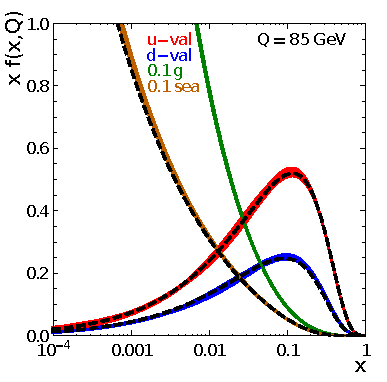
\includegraphics[width=0.5\textwidth]{CT10_2}}
   \caption[CT10 NNLO parton distribution functions.]{CT10 NNLO parton distribution functions for up and down quarks,
   gluons and sea quarks, given at two different factorisation scales: (a) Q = \SI{3.16}{\GeV}, (b) Q =
   \SI{85}{\GeV} \autocite{CT10_NNLO}.}
   \label{fig:CT10_PDFs}
\end{figure}

The total \ttbar production cross section for hard scattering processes in hadron collisions can be calculated to a
fixed order as \autocite{Sterman1986, primer_LHC}:
\begin{equation}
\sigma^{\ttbar} (s,\mtop^2) = \sum_{i,j} \int dx_i dx_j f_i(x_i, \mu_f^2) f_j(x_j,\mu_f^2) \hat{\sigma}_{i,j
\rightarrow \ttbar} (\hat{s}, \mtop^2, \alpha_S(\mu_r^2)),
\end{equation}
where the indices $i,j$ run over the incoming partons (gluons and quark-antiquark pairs), $x_{i,j}$ are the momentum
fractions of the incoming partons, $f_{i,j}$ are their parton distribution functions, and $\hat{\sigma}_{i,j
\rightarrow \ttbar}$ is the cross section of interacting partons, which depends on the parton centre of mass energy
$\hat{s} \sim x_i x_j s$, the top quark mass \mtop, and the QCD strong coupling constant $\alpha_S$. The latter
parameter is evaluated at renormalisation scale $\mu_r$. The top quark mass \mtop, as discussed in
Section~\ref{ss:top_mass}, also depends on the choice of renormalisation scheme and scale $\mu_r$.

The results of the most recent theoretical calculation of \ttbar cross section performed with
next-to-next-to-leading-order (NNLO) QCD corrections \autocite{NNLO_ttbar} are given in
Table~\ref{tab:ttbar_NNLO_xsections}. The cross section has also been measured by CMS and ATLAS experiments at the LHC
-- the comparison of these measurements with the theoretical prediction is shown in
Figure~\ref{fig:xsections_comparison_NNLO}.

\begin{table}[!hbp]
\centering
\caption{Theoretical predictions for \ttbar production cross section at
different LHC centre of mass energies, calculated at
next-to-next-to-leading-order (NNLO) \autocite{NNLO_ttbar}. The scales uncertainty corresponds to the choice of factorisation and renormalisation scales. }
\label{tab:ttbar_NNLO_xsections} 
\begin{tabular}{lrrr}
 \toprule
 $\sqrt{s}$ & $\sigma_\textrm{total}$ [\pb] & scales [\pb] & PDF [\pb] \\
 \midrule
 \SI{7}{\TeV}  & 172.0 & ${}^{+4.4~(2.6\%)}_{-5.8~(3.4\%)}$ & ${}^{+4.7~(2.7\%)}_{-4.8~(2.8\%)}$ \\
 \addlinespace[0.5em]
 \SI{8}{\TeV}  & 245.8 & ${}^{+6.2~(2.5\%)}_{-8.4~(3.4\%)}$ & ${}^{+6.2~(2.5\%)}_{-6.4~(2.6\%)}$ \\
 \addlinespace[0.5em]
 \SI{14}{\TeV} & 953.6 & ${}^{+22.7~(2.4\%)}_{-33.9~(3.6\%)}$ & ${}^{+16.2~(1.7\%)}_{-17.8~(1.9\%)}$ \\
 \bottomrule
\end{tabular}
\end{table}

\begin{figure}[bhtp]
   \centering
   {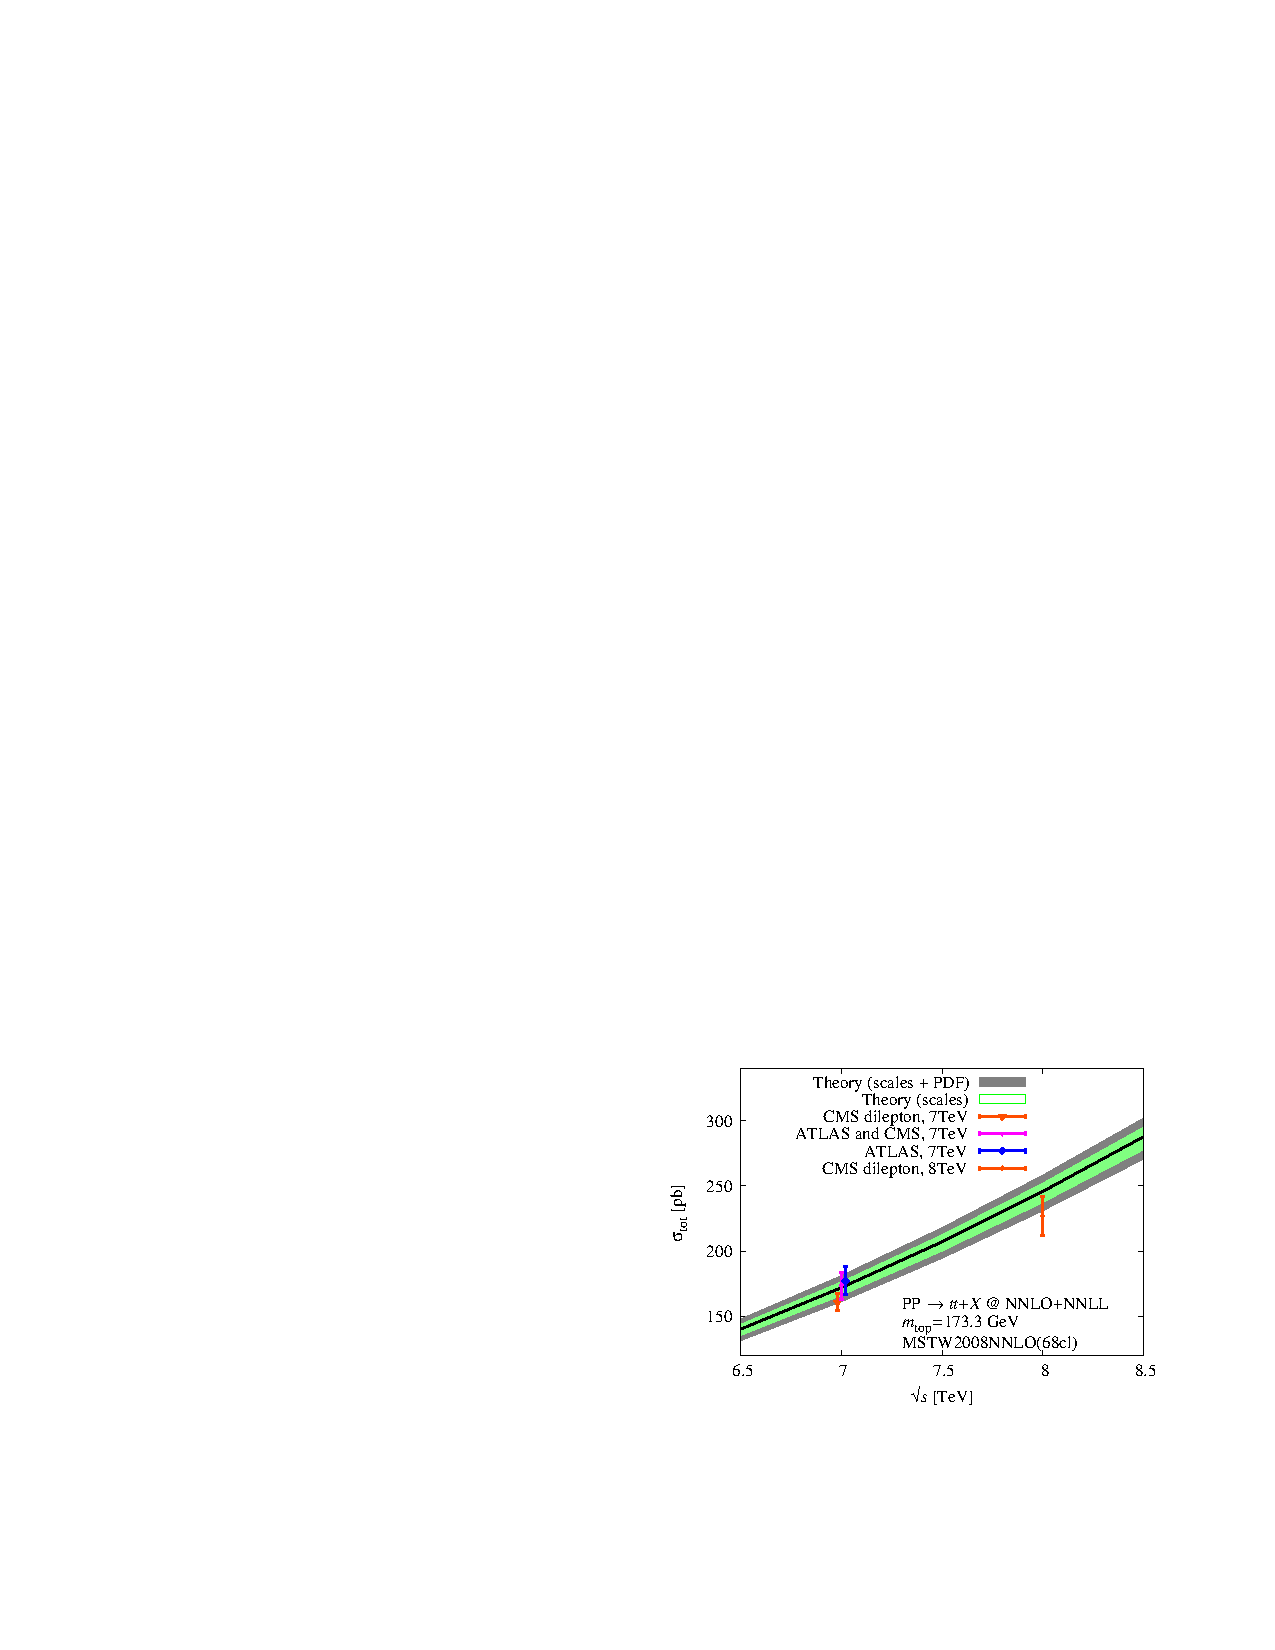
\includegraphics[width=0.7\textwidth]{xsections_comparison_NNLO}}
   \caption[Measurement of the \ttbar production cross section]{Measurement of the \ttbar production cross section at
   centre of mass energies of \SI{7}{\TeV} and \SI{8}{\TeV} by ATLAS and CMS experiments, compared with the theoretical
   prediction \autocite{NNLO_ttbar}.}
   \label{fig:xsections_comparison_NNLO}
\end{figure}

An abundance of top quark events at the LHC allows measurements of differential \ttbar production cross section with
respect to many different variables. These measurements provide important tools for validation of various MC models and
higher-order QCD calculations of \ttbar production. Since the very same models are used in BSM searches where \ttbar
events represent a major background, such validation is of great importance. Moreover, these measurements can themselves
be sensitive to signal contributions from new physics.

Normalised differential cross section in each bin $i$ of an observed variable $\mathrm{X}$ is given by:
\begin{equation}
\label{eq:normalised_differential_xsection_theory}
\frac{1}{\sigttbar^\mathrm{tot}} \frac{\mathrm{d}\sigma_i}{\mathrm{d} \mathrm{X}} = \frac{1}{\sigttbar^\mathrm{tot}}
\frac{x_i}{\Delta \mathrm{X}_i \calL},
\end{equation}
where $x_i$ is the number of signal events in data after subtraction of background, corrected for detector efficiency,
acceptance and migration between the bins of variable $\mathrm{X}$; $\calL$ is the total integrated luminosity; $\Delta
\mathrm{X}_i$ is the variable bin width; and $\sigttbar^\mathrm{tot}$ is the total \ttbar production cross section. The
normalisation is performed in order to cancel the systematic uncertainties that are correlated between the bins of
variable $\mathrm{X}$.

Both ATLAS and CMS collaborations have delivered a range of differential \ttbar production cross section measurements
\autocite{ATLAS_diff_xsections_7TeV, CMS_diff_xsections_7TeV}. For instance, Figure~\ref{fig:ATLAS_CMS_diff_xsections}
shows the normalised differential cross section with respect to the invariant mass of \ttbar pair ($m_{\ttbar}$),
measured by ATLAS and CMS collaborations using the $\sqrt{s} = \SI{7}{\TeV}$ LHC data. These measurements require a full
kinematic reconstruction of the semileptonic \ttbar decay in order to accurately calculate the $m_{\ttbar}$ variable.
Other variables requiring the kinematic reconstruction include the transverse momenta of top quarks decaying either
leptonically or hadronically, their rapidities, etc.

\begin{figure}[hbtp]
   \centering
   \subfloat[]{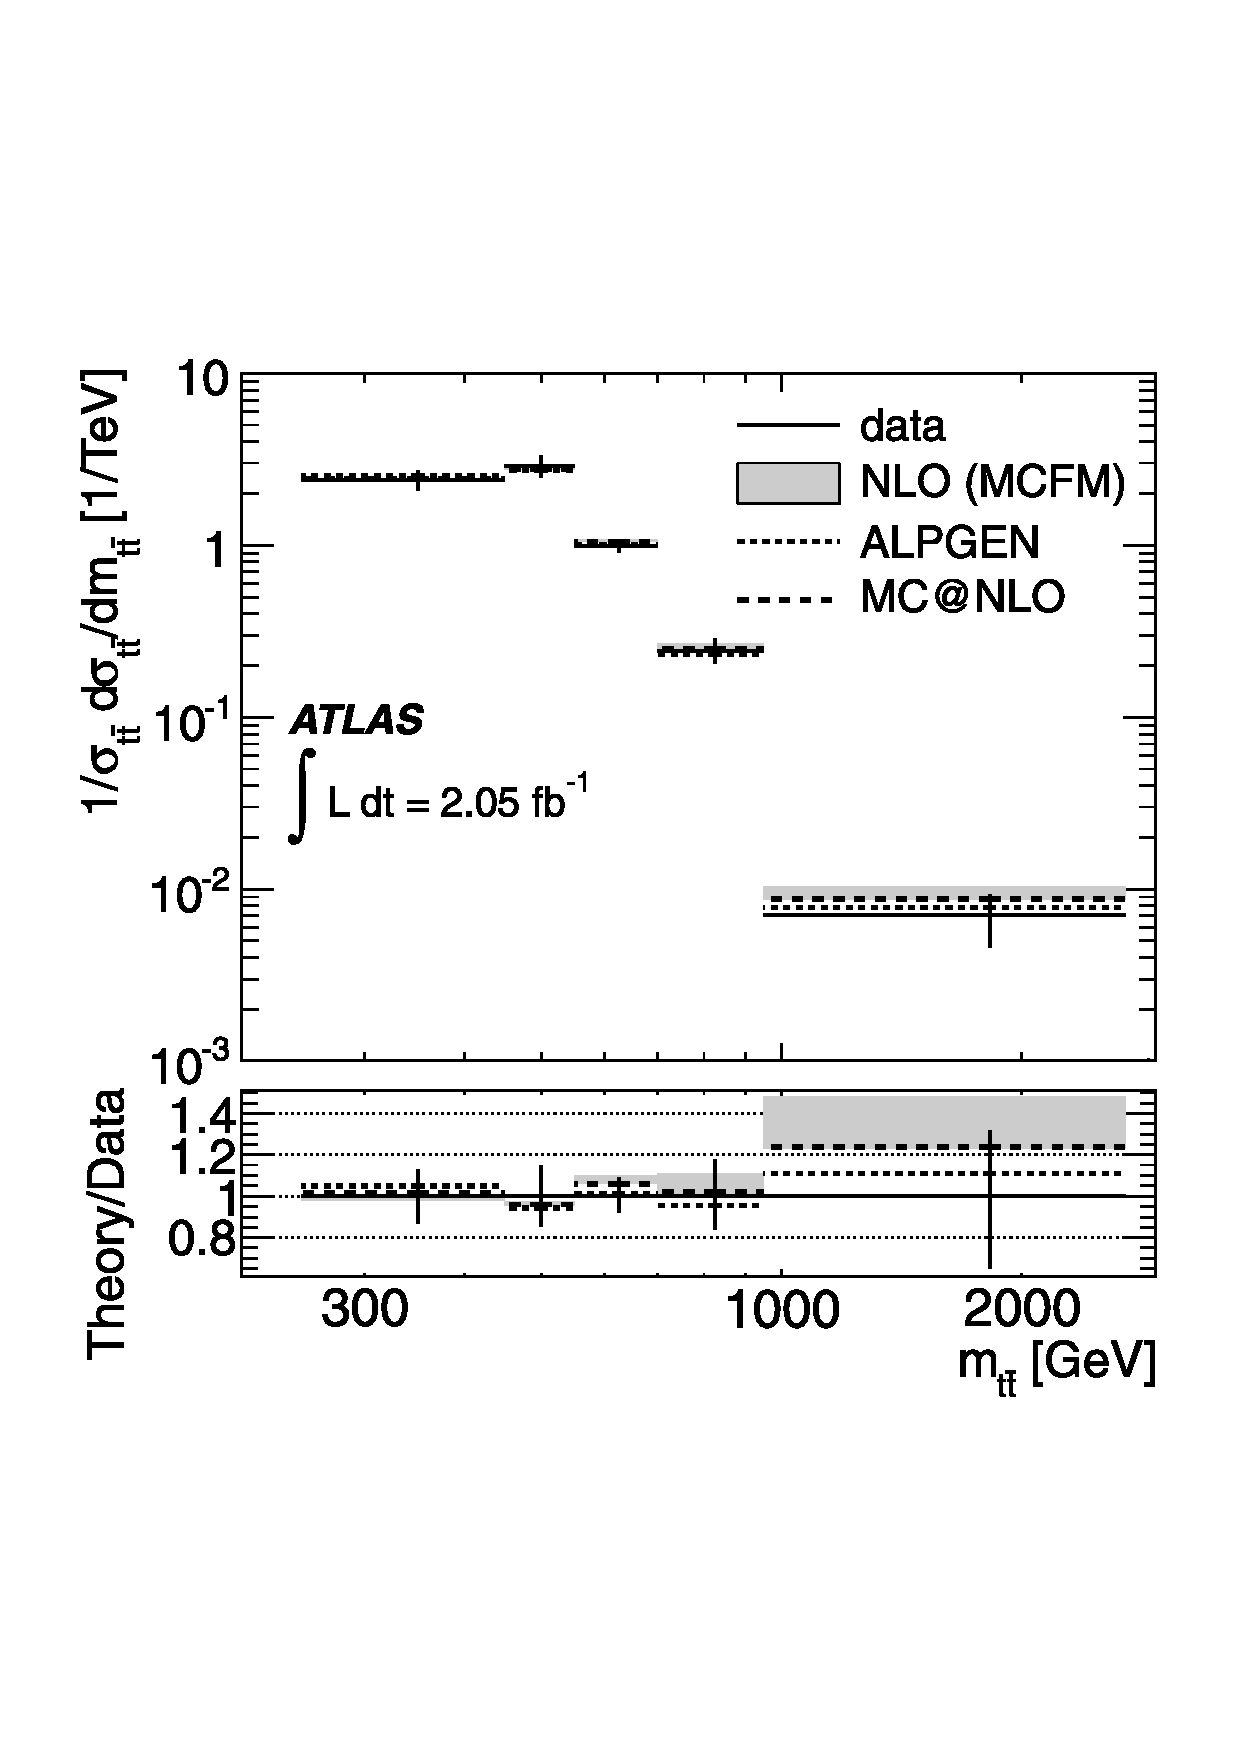
\includegraphics[width=0.5\textwidth]{ATLAS_diff_xsection_mtt}}
   \subfloat[]{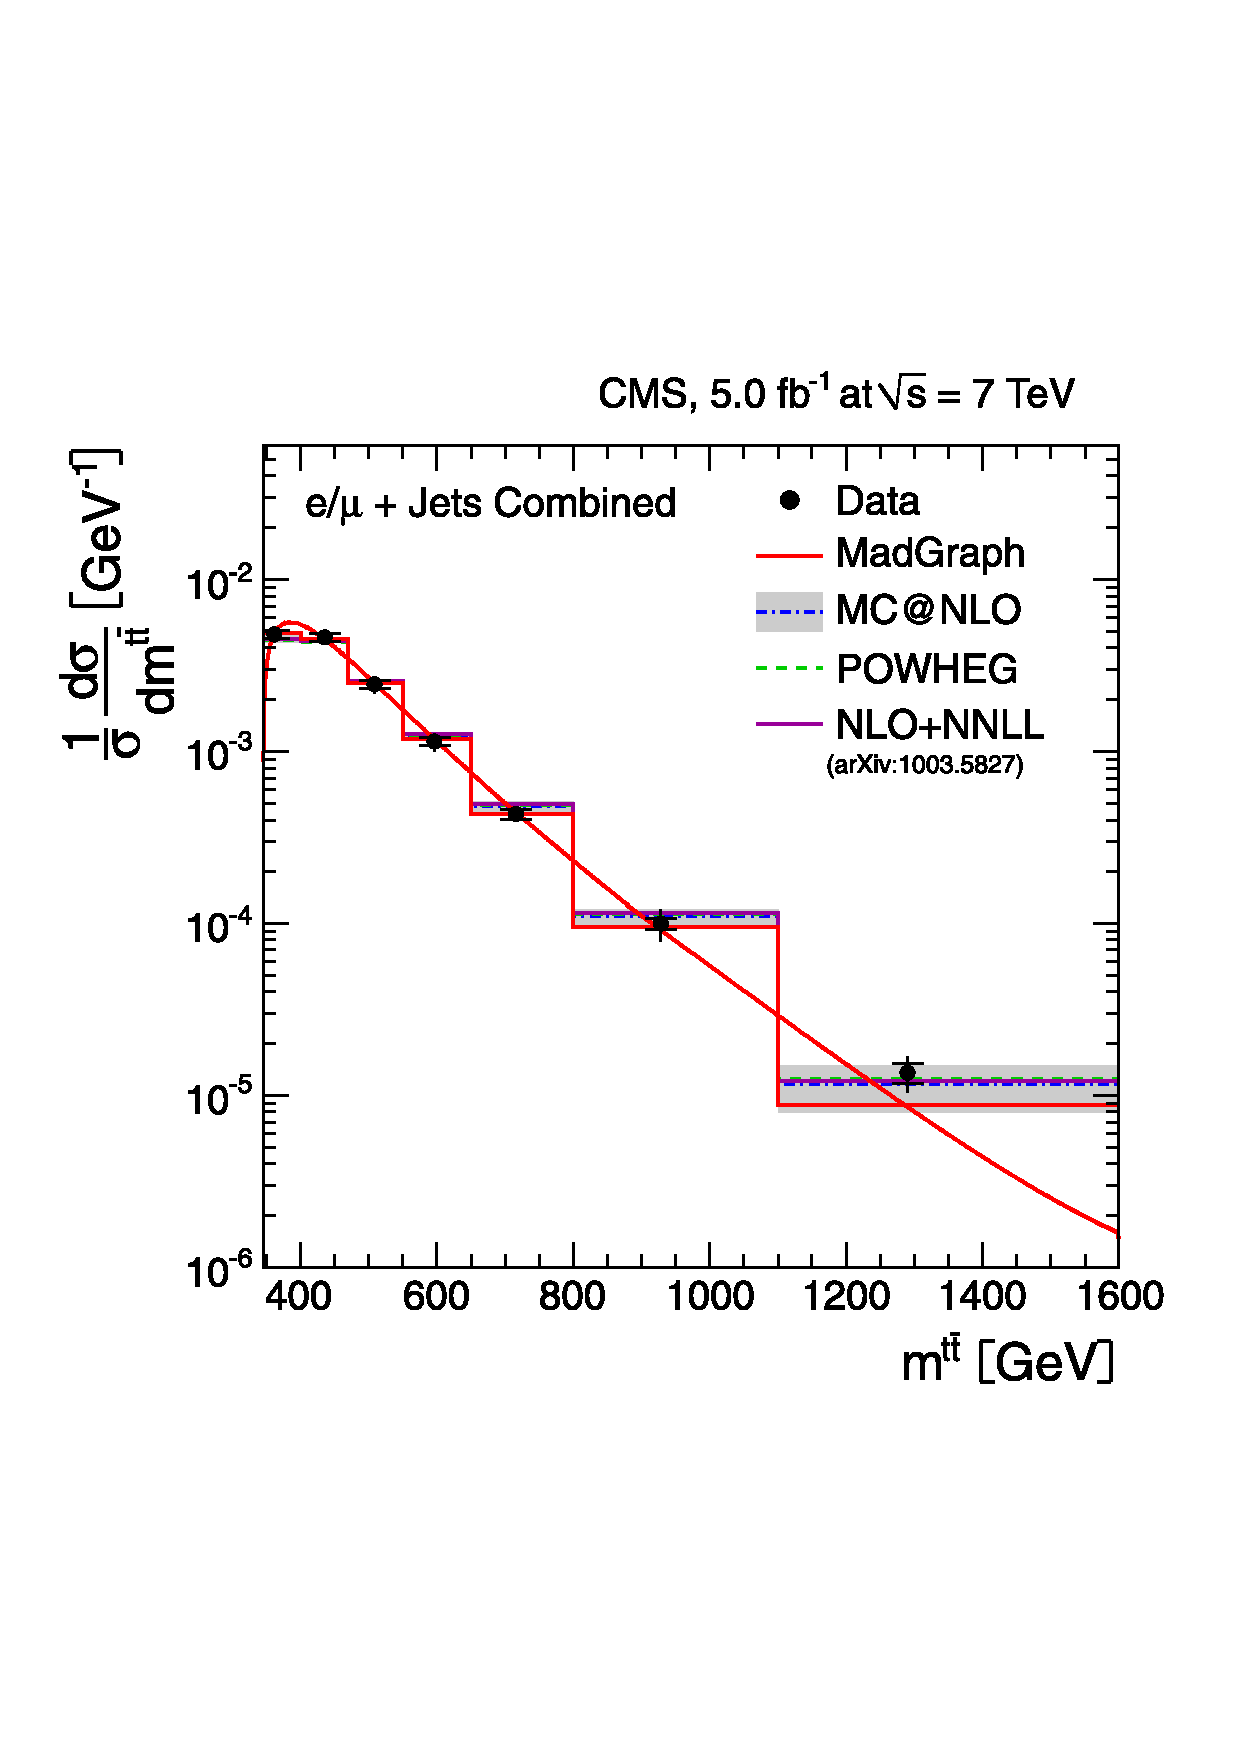
\includegraphics[width=0.5\textwidth]{CMS_diff_xsection_mtt}}
   \caption[Normalised differential \ttbar production cross section measurements by ATLAS and CMS
   collaborations]{Normalised differential \ttbar production cross section measurements in the $l+$jets channel with
   respect to the invariant mass of a top quark pair. (a) ATLAS measurement \autocite{ATLAS_diff_xsections_7TeV}, (b)
   CMS measurement \autocite{CMS_diff_xsections_7TeV}.}
   \label{fig:ATLAS_CMS_diff_xsections}
\end{figure}

In this thesis, the \ttbar differential cross section is measured with respect to so-called event-level (or global)
variables, not requiring a kinematic reconstruction of the \ttbar decay -- for example, missing transverse energy (\MET)
or total hadronic activity (\HT) in the event (see Section~\ref{ss_xsection:variables}). The main advantage of these
measurements is the absence of the systematic uncertainty associated with the kinematic reconstruction. Additionally,
signs of new physics scenarios could be revealed in the tails of these distributions. For example, an associative
production of a \ttbar pair with some new resonance ($\ttbar+\mathrm{X}$) decaying invisibly can show up in the tail of
the missing transverse energy distribution.

\section{Summary}
In this chapter, an overview of the Standard Model has been presented. The concept of gauge principle and its
applications in the electroweak theory and the Quantum Chromodynamics, as well as the mechanism of the electroweak
symmetry breaking have been briefly described. Shortcomings of the Standard Model and some models proposing the
solutions have been mentioned. Finally, an introduction to the top quark physics has been given, with pointing out the
relevance and importance of the top quark mass and differential cross section measurements presented in this thesis.

%%% Local Variables: 
%%% mode: latex
%%% TeX-master: "../thesis"
%%% End: 

\end{fmffile}
%!TEX root = ../thesis.tex

\chapter{The LHC and the CMS detector}
\label{c:detector}
\ifpdf
    \graphicspath{{03_Detector/plots/}}
\else
    \graphicspath{{03_Detector/plots/EPS/}{03_Detector/plots/}}
\fi

\section{The Large Hadron Collider}
\label{s:LHC}

The LHC \autocite{LHC} is currently the largest and the most powerful particle accelerator ever built. It is installed
in the \SI{26.7}{\km} tunnel that was originally constructed for the LEP accelerator in the 1980s. The tunnel lies at a
depth of \SIrange{45}{170}{\metre} underground between the Jura mountain and Lake Geneva, being the main part of the
CERN accelerator complex.

The machine is designed to accelerate proton beams and provide collisions at a centre of mass energy of $\sqrt s =$
\SI{14}{\TeV}. Unlike particle-antiparticle colliders, the LHC requires two rings with opposite magnetic dipole fields
in order to maintain and collide two counter-rotating proton beams. Since the tunnel was originally designed for the
electron-positron LEP, it has an internal diameter of \SI{3.7}{\metre} which is not enough to install two separate
independent rings. Therefore, a twin-bore magnet design was adopted \autocite{Blewett}, which resulted in substantial
cost savings.

\begin{figure}[!htbp]
  \begin{center}
    \leavevmode
    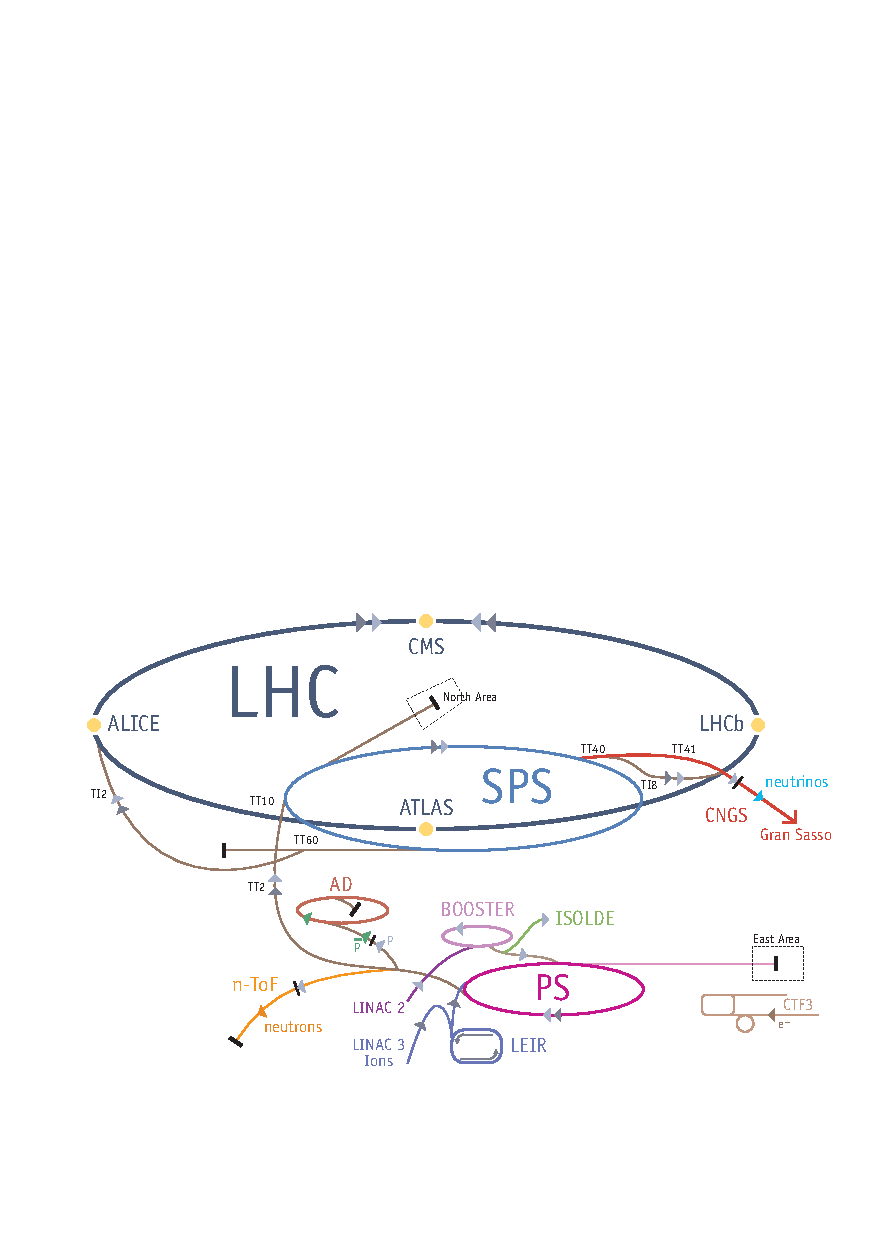
\includegraphics[width=\columnwidth]{LHC}
    \caption{CERN accelerator complex.}
    \label{LHC}
  \end{center}
\end{figure}

A schematic view of the LHC accelerator chain is shown in Figure~\ref{LHC}. Initially, the protons are obtained by
stripping orbiting electrons from hydrogen atoms. Then they are injected into the linear accelerator LINAC2 to reach the
energy of \SI{50}{\MeV} and enter the Proton Synchrotron Booster (PSB). The booster accelerates them to \SI{1.4}{\GeV}
and passes the beam to the Proton Synchrotron (PS) where the energy rises to \SI{25}{\GeV}. In the next step, protons
enter the Super Proton Synchrotron (SPS) where they are accelerated to \SI{450}{\GeV}. Finally, the beam is transferred
to the LHC in both clockwise and anti-clockwise directions where it takes about 20 minutes to reach the design
\SI{7}{\TeV} energy (per beam).

\textit{[add the number of magnets, total energy stored, number of bunches, bunch spacing etc.?]}

The LHC has four interaction points, providing collisions to four major experiments. Two of them, CMS and ATLAS, are
multi-purpose high-luminosity experiments with a peak luminosity of $L = $ \SI{d34}{\cm^{-2} s^{-1}}. The other two
experiments operate at low luminosities and have more specific physics goals: LHCb studies b-meson decays, and Alice is
a dedicated heavy ion experiment.

The instantaneous luminosity of a collider can be calculated as
\begin{equation}
	L = \frac{n_1 n_2 f}{4 \pi \sigma_x \sigma_y},
\end{equation}
where $n_1$ and $n_2$ are the numbers of particles in each of the colliding bunches, $f$ is the revolution frequency,
$\sigma_x$ and $\sigma_y$ are the horizontal and vertical beam sizes, assuming the two beams have the same size.

The number of events generated in the collisions per second is given by
\begin{equation}
	N_{events} = L \times \sigma,
\end{equation}

where $\sigma$ is the cross section of the process under study.

\textit{[add the plots with cross sections and production rates?]}

The LHC started operating on the 10th of September 2008, with the first beams fully circulating in both rings. However,
only 9 days later a magnet quench occurred in two sectors of the tunnel, which was caused by an electrical fault due to
a bad connection between two magnets. A consequent liquid helium explosion damaged a total of 53 superconducting
magnets. Over a year was spent on repairs and tests, and the first collisions were recorded on the 23rd of November 2009
at a centre of mass energy of \SI{0.9}{\TeV}. The following few months showed the continuous ramp up of the beam
energies up to \SI{3.5}{\TeV} per beam which was achieved on the 30rd of March 2010 when the LHC physics programme
started.

Throughout the rest of 2010, the two general-purpose LHC experiments (CMS and ATLAS) recorded approximately
\SI{40}{\invpb} of data, which resulted in the first measurements of various physics processes at the LHC. The following
year became the main \SI{7}{\TeV} data-taking period, with about \SI{5}{\invfb} of data recorded by ATLAS and CMS. On
the 5th of April 2012 the centre of mass energy was increased to 8 TeV, and July of 2012 marked the first major
discovery of a new boson which was later shown to be consistent with the Standard Model Higgs boson, according to
approximately \SI{21.8}{\invfb} of data recorded until early 2013. A long shut-down is planned for the following two
years with various upgrades scheduled. The next physics run is expected in 2015 with the beam energy increased up to 6
or \SI{7}{\TeV}.

\textit{[add any upgrade details and distant future plans, like SLHC?]}

\section{The CMS Detector}
\label{s:CMS}

The Compact Muon Solenoid \autocite{CMS} is a general-purpose detector designed to carry out precise measurements of the
Standard Model and searches for physics beyond it. The primary design requirement was the ability to discover the nature
of electroweak symmetry breaking, and the first observation of a Higgs boson was obtained in the Summer of 2012
\autocite{CMS_Higgs}.

The detector is installed at one of the LHC interaction points (Point 5) at about \SI{100}{\metre} underground near the
French village of Cessy, between the Jura mountains and Lake Geneva. The overall dimensions of the CMS detector are a
length of \SI{21.6}{\metre}, a diameter of \SI{14.6}{\metre} and a total weight of \SI{12500}{\tonne}.

\begin{figure}[htbp]
  \begin{center}
    \leavevmode
    \includegraphics[width=\columnwidth]{CMS}
    \caption{Sectional view of the CMS detector.}
    \label{CMS}
  \end{center}
\end{figure}

The sectional view of CMS is shown in Figure~\ref{CMS}. In the centre of the detector, tracking and calorimetry systems
are surrounded by the superconducting solenoid. On the outermost part of it the magnetic flux is returned through the
iron yoke in which the muon system is also integrated. All the sub-systems are discussed in the following sections in
more detail.

The cylindrical shape of the CMS detector dictates using a cylindrical coordinate system, with the origin centred at the
interaction point, the $x$-axis pointing towards the centre of the LHC ring, the $y$-axis pointing upwards and the
$z$-axis pointing along the beamline in the anti-clockwise direction. The azimuthal angle $\phi$ is measured from the
$x$-axis in the transverse ($x-y$) plane and the polar angle $\theta$ is measured from the $z$-axis. The radial distance
to the beamline is denoted by $r$. Pseudorapidity is defined as:
\begin{equation}
  \eta = - \ln{\tan{\frac{\theta}{2}}}.
\end{equation}
This implies that the particles moving in the transverse plane (perpendicular to the beamline) have a pseudorapidity of
0, whereas the beam direction has an infinite pseudorapidity. Considering the cylindrical shape of the detector, it has
barrel and endcap regions, with the transition occurring at $\eta \sim 1.4$. The momentum and energy transverse to the
beamline are denoted by $p_T$ and $E_T$ respectively; the imbalance of the energy measured in the transverse plane,
called missing transverse energy, is denoted by \ETm.

\subsection{Inner Tracking System}
\label{ss:tracker}
The tracking system lies in the heart of the CMS detector and is the closest to the interaction point where the particle
flux has the highest value. This imposes demanding requirements on the configuration of the system. At design luminosity
of $L = $ \SI{d34}{\cm^{-2} s^{-1}} with the bunch spacing of \SI{25}{\ns}, an average of \num{1000} particles from
about \num{25} proton-proton interactions (pile-up vertices) is expected to traverse the tracker for each bunch
crossing. However, up until the long shutdown a bunch spacing of \SI{50}{\ns} was used, which meant a higher number of
protons in each bunch leading to approximately twice the number of pile-up vertices. Therefore, in order for the
particle tracks to be identified reliably and separately for each bunch crossing, the tracker requires very fine
granularity and fast response parameters. Another complication caused by the intense particle flux is the severe
radiation damage, so the tracker has to be highly resilient in operating in the harsh environment for a reasonable
lifetime.

To meet these requirements on granularity, response time and radiation resilience, the tracker design was chosen to be
based on silicon detector technology. Although capable of meeting such conditions, this technology has a disadvantage of
a high power density of on-detector electronics. This implies the necessity of an efficient cooling system. Moreover, a
large amount of dense material interacting with the particles leads to higher multiple scattering, bremsstrahlung,
photon conversions and nuclear interactions. Therefore, there are complications in the reconstruction of the tracks,
meaning some loss of efficiency and precision. This will be discussed in detail later on in the object reconstruction
section.

\begin{figure}[htbp]
  \begin{center}
    \leavevmode
    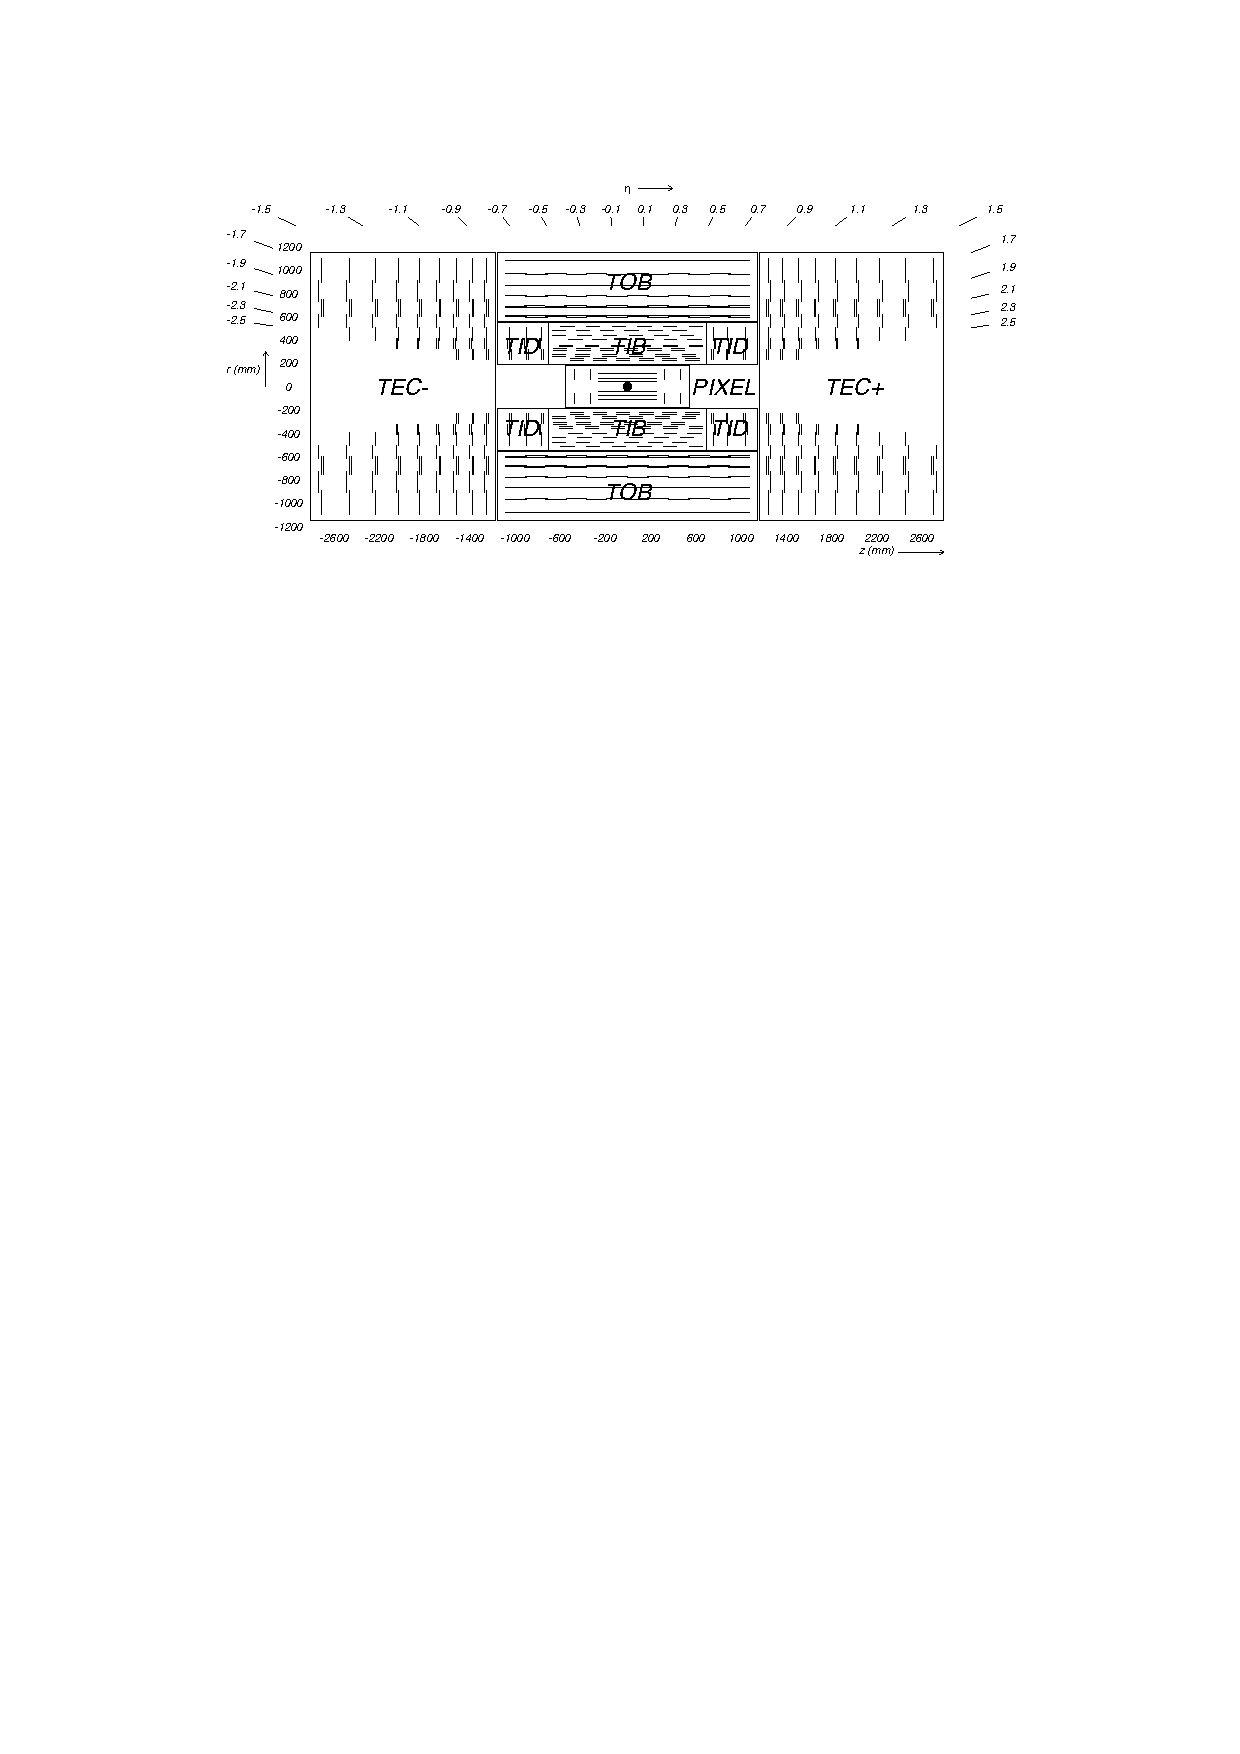
\includegraphics[width=\columnwidth]{tracker}
    \caption{Cross-section of the CMS tracker system \autocite{CMS}.}
    \label{Tracker}
  \end{center}
\end{figure}

Figure~\ref{Tracker} shows the overall layout of the tracking system. It consists of the inner pixel detector, located
in the vicinity of the interaction point, and silicon strip tracker detectors: inner barrel and disks (TIB and TID),
outer barrel (TOB) and endcaps (TEC). The geometrical acceptance of the tracker system goes up to \abs\eta \num{<2.5}.
The outer radius of the CMS tracker reaches approximately \SI{110}{\cm}, and its total length is about \SI{540}{\cm}.

The pixel detector consists of three layers of pixel sensors at radii of \SIlist{4.4;7.3;10.2}{\cm} from the beamline in
the barrel region. In addition there are two endcap disks on each side at \abs z $=$ \SIlist{34.5;46.5}{\cm}. The pixel
size equals \num{100x150} \si{\micron\squared} in $r \phi \times z$ coordinates. The pixel detector has 66 million
pixels and the total area of about \SI{1}{\m\squared}.

The silicon strip tracker consists of several layers of silicon microstrip detectors. It covers the region between
\SIrange{20}{110}{\cm} in radius and extends up to \SI{+-280}{\cm} in the z direction. The Tracker Inner Barrel (TIB) is
made out of 4 layers and the Tracker Outer Barrel (TOB) has 6 layers in it. The tracker endcaps (TEC) comprise 9 disks,
and there are also the tracker inner disks (TID) that consist of 3 disks filling the gap between TIB and TEC as shown in
Figure~\ref{Tracker}. There are \num{9.3} million silicon strips covering the area of about \SI{200}{\m\squared}. The
silicon sensors' thickness varies between \num{320} and \SI{500}{\micron} and the strip pitch varies from
\SI{80}{\micron} in the TIB to \SI{180}{\micron} in TOB and TEC.

\begin{figure}[!htbp]
  \begin{center}
    \leavevmode
    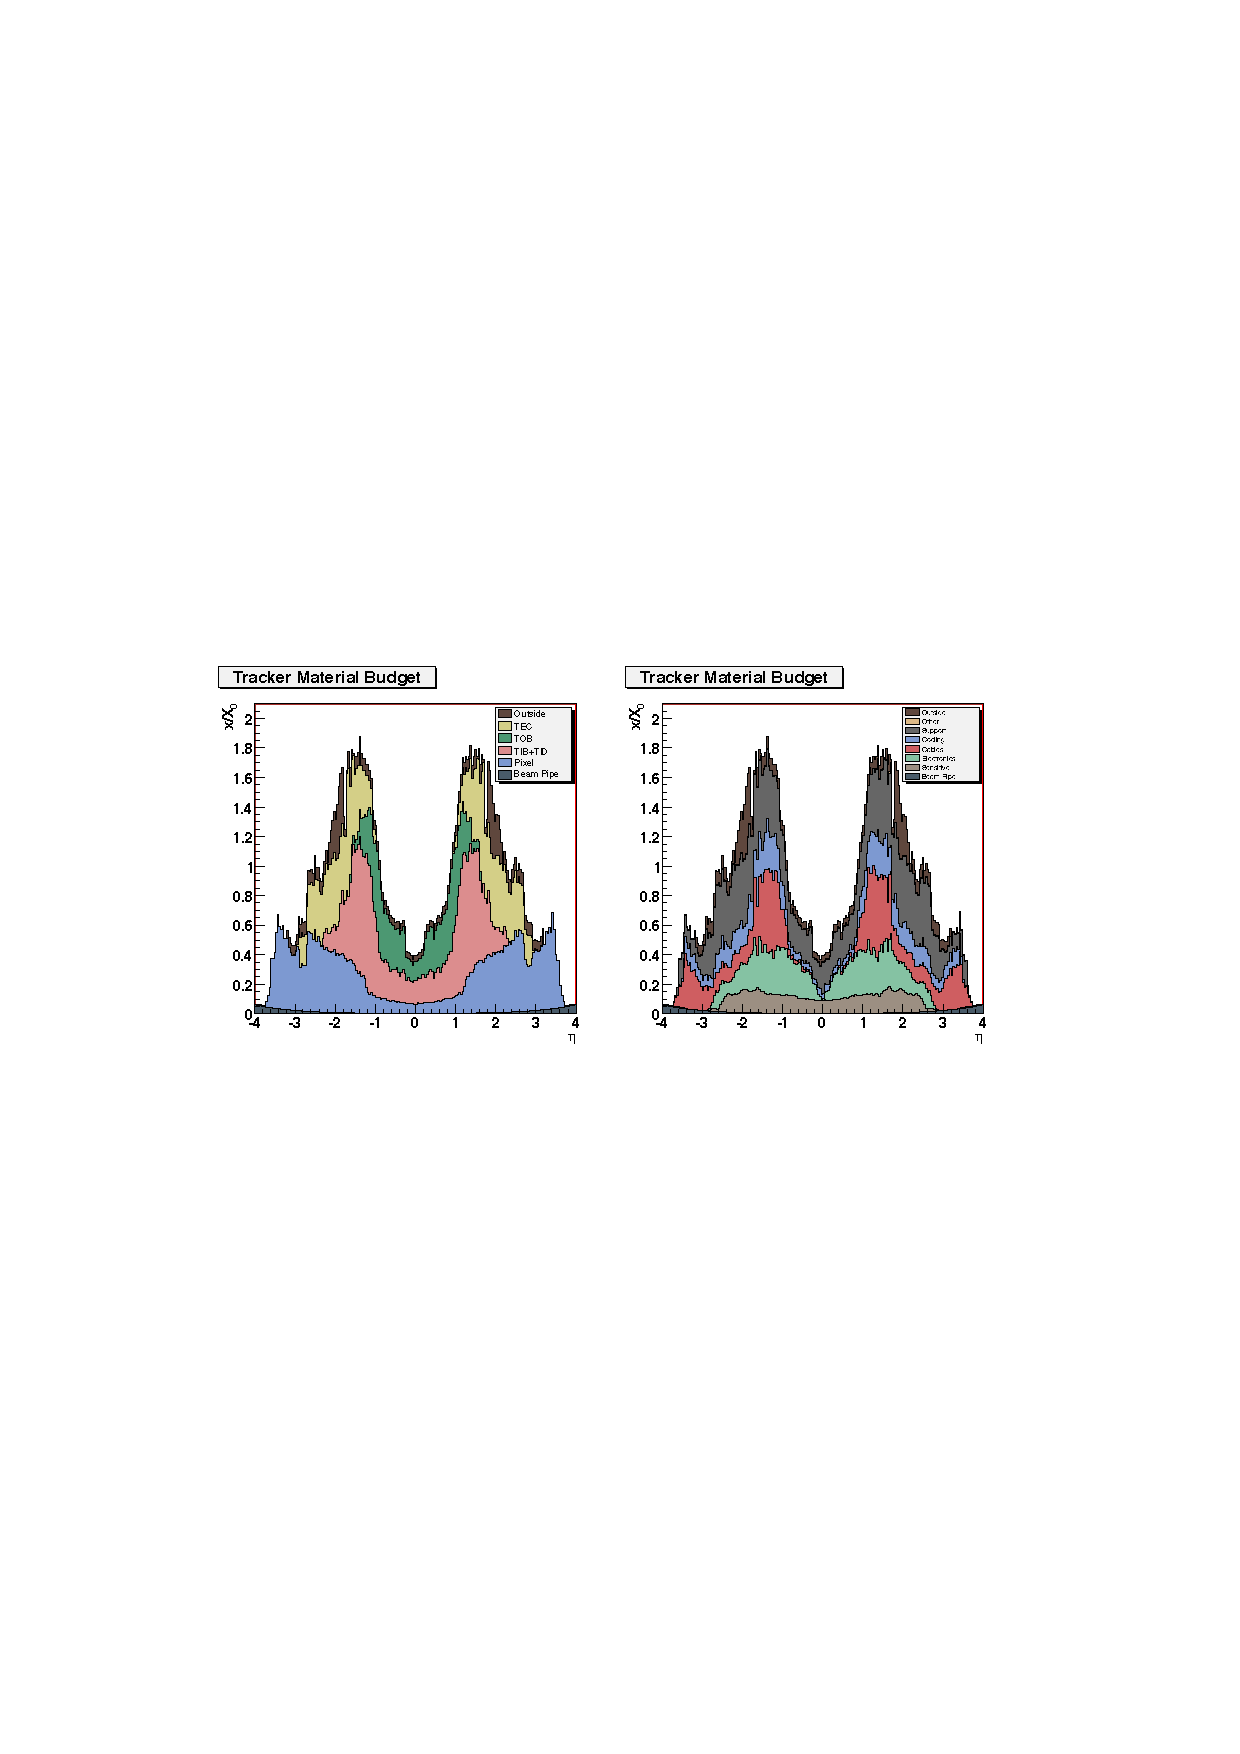
\includegraphics[width=\columnwidth]{tracker_material_budget}
    \caption{Material budget as a function of pseudorapidity $\eta$ for the different sub-detectors of the tracker
    (left) and broken down into the functional contributions (right), in units of radiation length \autocite{CMS}.}
    \label{tracker_material_budget}
  \end{center}
\end{figure}

%update with http://cms.cern.ch/iCMS/jsp/analysis/admin/analysismanagement.jsp?awg=TRK&dataset=All&awgyear=2011

The silicon detectors of the tracker, the readout electronics and support structure form a considerable amount of
material for the particles traversing from the interaction point. Figure~\ref{tracker_material_budget} \autocite{CMS}
shows the material budget of the CMS tracker in units of radiation lengths\footnote{A material's radiation length is the
mean distance over which a high-energy electron loses all but $1/e$ of its energy by bremsstrahlung; this is equal to
\num{7/9} of the mean free path for pair production by a high-energy photon.} ($X_0$). It grows from about \num{0.4}
$X_0$ to \num{1.8} $X_0$ in the barrel region, and then decreases to about \num{1} $X_0$ in the endcaps. This causes a
substantial conversion rate for photons and electrons in the tracker material; it also will be discussed in more detail
in the electron reconstruction section.

\textit{[perhaps need to add the $p_T$ resolution plots]}

\subsection{Electromagnetic Calorimeter}
The next detector subsystem which is surrounding the tracker is the electromagnetic calorimeter, or ECAL. It is of a
primary importance for the analyses described in this thesis, as it provides information for the electron and positron
reconstruction. Combination of this information with that from the tracking system must ensure a precise measurement of
electron position and momentum, and also sufficient background removal. It has to effectively distinguish the energy
deposit shape of an electromagnetic particle from the one of a hadronic particle, which requires good segmentation and
high resolution.

ECAL is a hermetic, high-granularity, high-resolution scintillating crystal calorimeter consisting of \num{61200} lead
tungstate ($\textrm{PbWO}_4$) crystals located in the central barrel region (\abs\eta $<1.479$), and \num{7324} crystals
in each of the two endcaps (\num{1.479} $<$\abs\eta\num{<3.0}). All crystals are followed by photodetectors reading and
amplifying their scintillation: avalanche photodiodes (APD) are used in the barrel, and vacuum phototriodes (VPTs) are
used in the endcaps. These different choices were caused by the configuration of the magnetic field and the expected
level of radiation.

\begin{figure}[!htbp]
  \begin{center}
    \leavevmode
    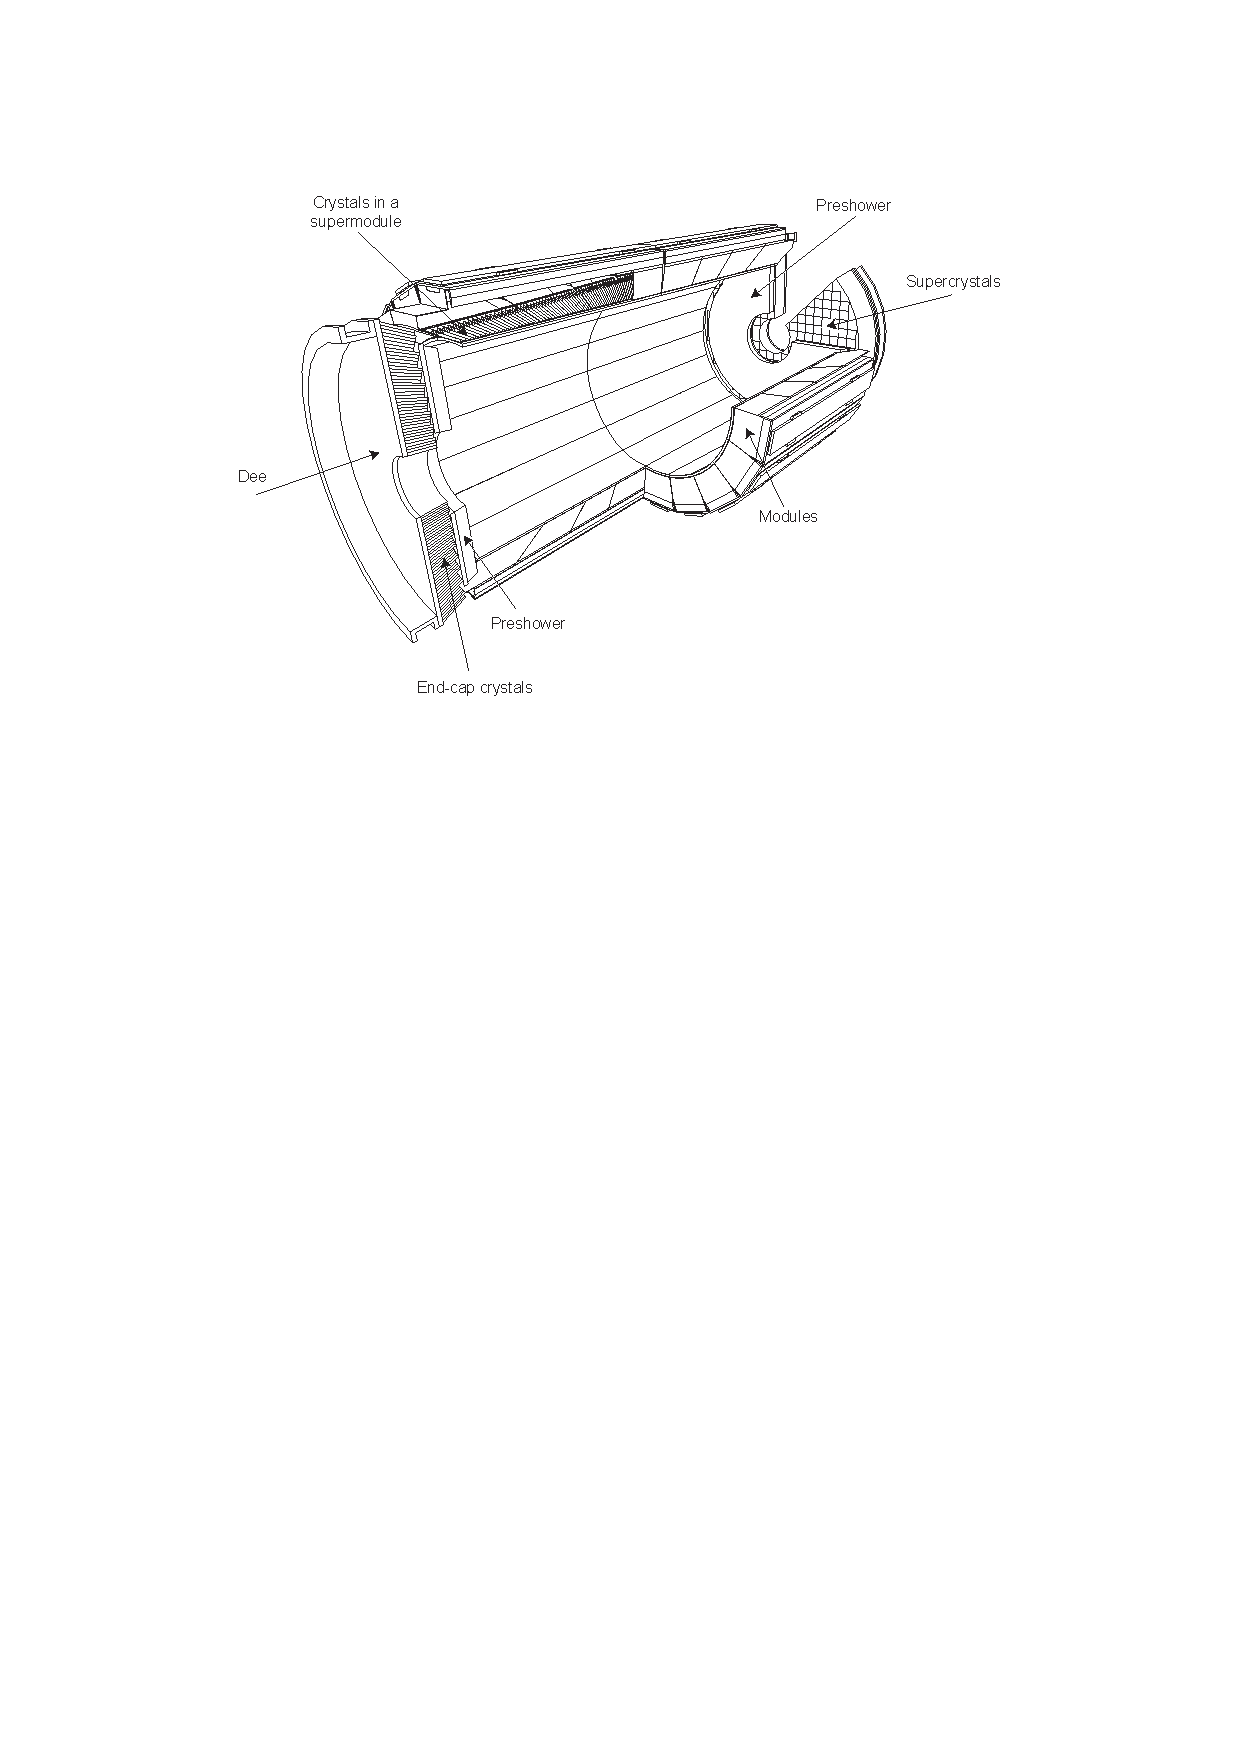
\includegraphics[width=\columnwidth]{ECAL}
    \caption{Layout of the CMS electromagnetic calorimeter \autocite{CMS}.}
    \label{ECAL}
  \end{center}
\end{figure}

The layout of the ECAL sub-detector is shown in Figure~\ref{ECAL}. An additional preshower detector is used in the
endcap region to lower the required detector depth. Its principal aim is to identify neutral pions in the endcaps, but
it also helps to distinguish neutral pions and electrons from minimum ionising particles and improves the position
determination of electrons and photons with high granularity.

\begin{table}[htbp]
\caption{ECAL crystal characteristics}
\label{ECAL_crystals}
\begin{center}
\begin{tabular}{|l|l|l|}
  \hline             
   & Barrel & Endcaps \\
  \hline
  number of crystals & \num{61200} & \num{14648} \\
  crystal cross-section in ($\eta$, $\phi$) & \num{0.0174 x 0.0174} & varies \\
  crystal cross-section at the front & \num{22x22} \si{\mm\squared} & \num{28.62x28.62} \si{\mm\squared} \\
  crystal cross-section at the rear & \num{26x26} \si{\mm\squared} & \num{30x30} \si{\mm\squared} \\
  crystal length & \SI{230}{\mm} (\num{25.8}$X_0$) & \SI{220}{\mm} (\num{24.7}$X_0$) \\
  \hline  
\end{tabular}
\end{center}
\end{table}

The main geometrical characteristics of the ECAL crystals are shown in Table~\ref{ECAL_crystals}. The choice of lead
tungstate was driven by the constraints of the CMS design. It is a very dense material (\SI{8.28}{g\per\cm\cubed}) with
a short radiation length of $X_0 = \SI{0.89}{\cm}$, which allows the calorimeter to fit inside the compact magnet. Lead
tungstate also has a small Moli\`ere radius\footnote{The Moli\`ere radius $R_\mu$ is a characteristic constant of a
material giving the scale of the transverse dimension of the fully contained electromagnetic showers initiated by an
incident high energy electron or photon. It is defined as the radius of a cylinder containing an average of
\SI{90}{\percent} of the shower's energy deposition.} of \SI{2.2}{\cm}, which allows a calorimeter with fine
granularity. Finally, the crystals emit \SI{80}{\percent} of their scintillation light in just \SI{25}{\ns}, however the
light yield is relatively low. At \SI{18}{\degreeCelsius}, about \num{4.5} photoelectrons per MeV are collected. The
dependence of the light yield on temperature requires a cooling system capable of keeping the crystal temperature stable
within \SI{+-0.05}{\degreeCelsius} to preserve energy resolution \autocite{CMS_TDR1}.

\begin{figure}[htbp]
  \begin{center}
    \leavevmode
    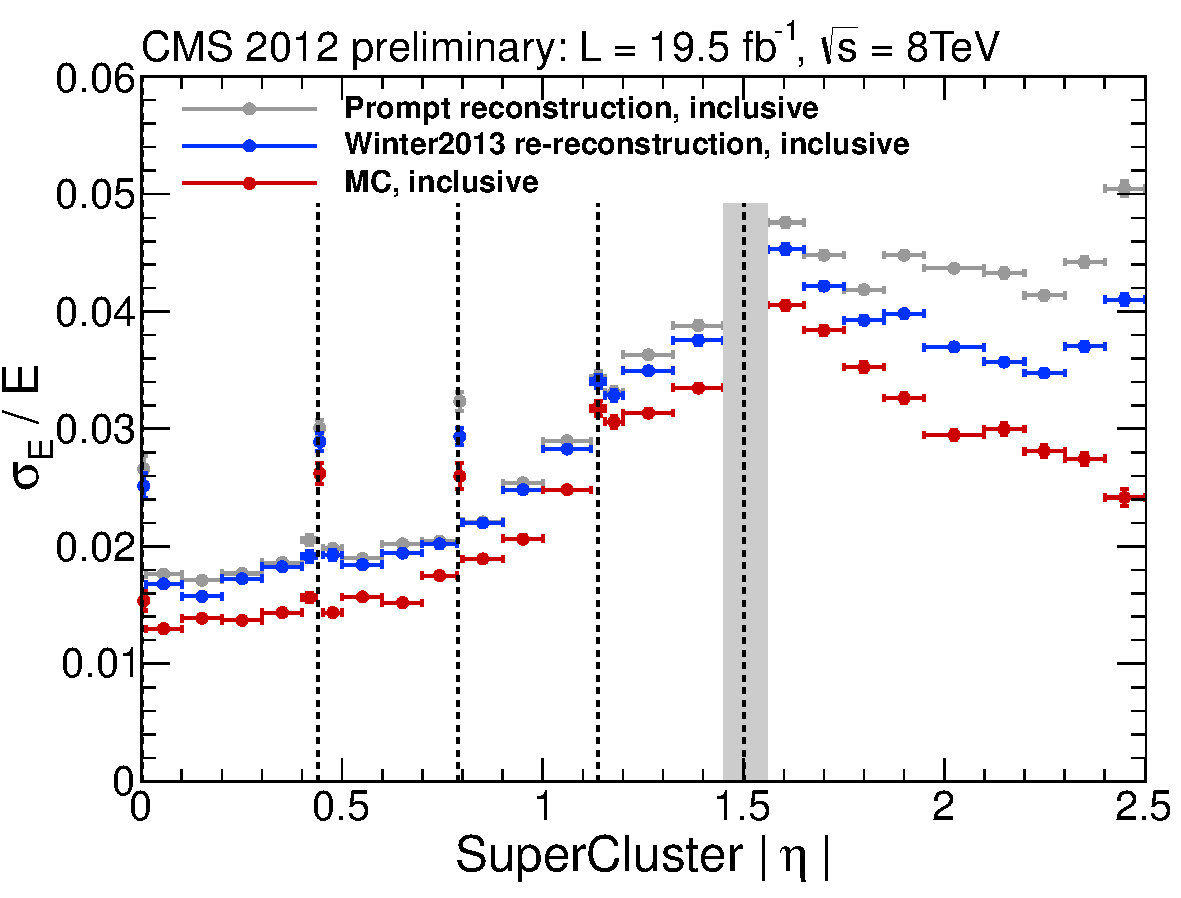
\includegraphics[width=0.7\columnwidth]{ECAL_resolution}
    \caption{ECAL energy resolution derived from the test beam measurements as a function of deposited energy. The
    stochastic, noise, and constant contributions are shown \autocite{CMS}.}
    \label{ECAL_resolution}
  \end{center}
\end{figure}

The energy-dependent resolution of the calorimeter can be parameterised as follows \autocite{CMS}:
\begin{equation}
  \left(\frac{\sigma}{E}\right)^2 = \left(\frac{S}{\sqrt E}\right)^2 + \left(\frac{N}{E}\right)^2 + C^2.
\end{equation}
where $S$ is the stochastic term, $N$ is the noise term, and $C$ is the constant term. Figure~\ref{ECAL_resolution}
shows the energy resolution measured using incident electrons, during the beam tests in 2004.

\subsection{Hadron Calorimeter}

The hadron calorimeter (HCAL) is the next sub-detector located mostly inside the solenoid and completing the CMS
calorimetry system. It is essential for the measurement of hadron jets and missing transverse energy.

\begin{figure}[htbp]
  \begin{center}
    \leavevmode
    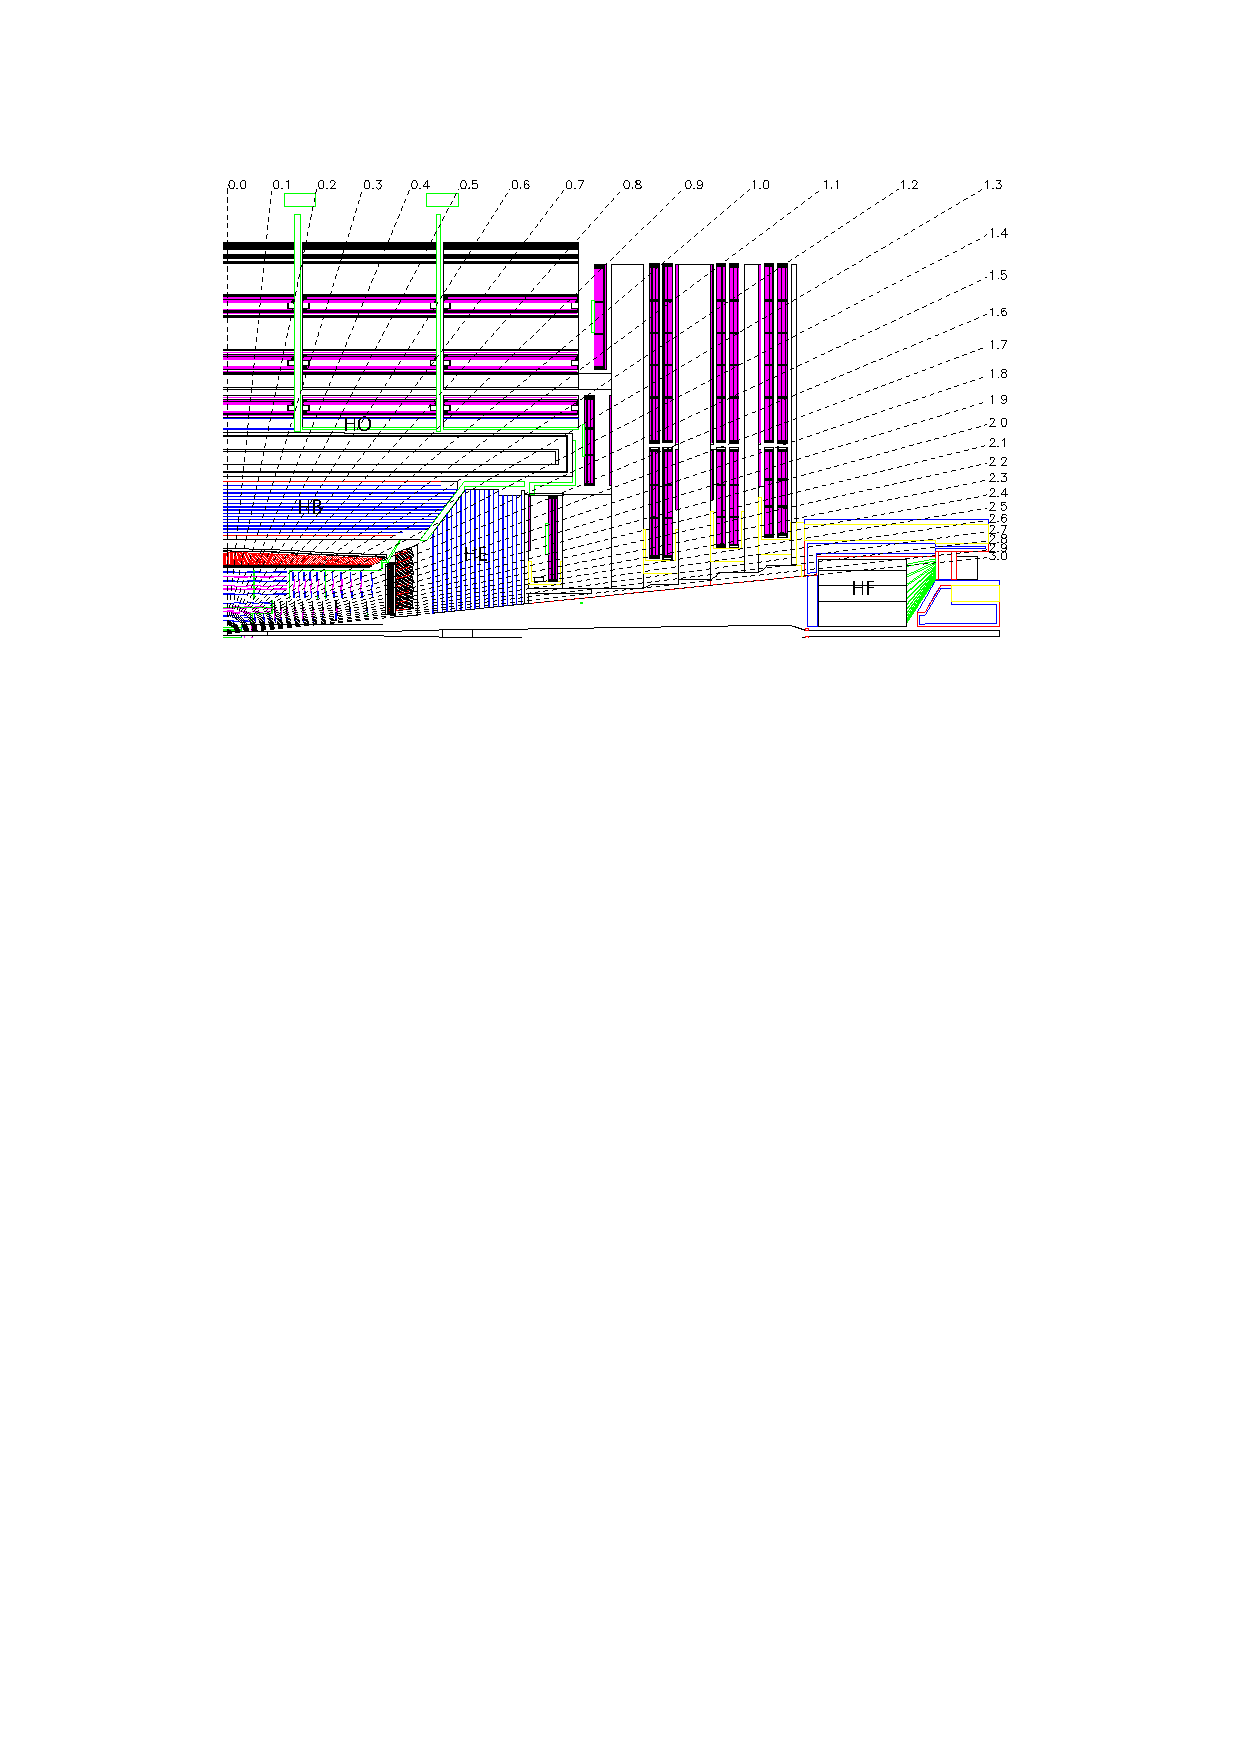
\includegraphics[width=\columnwidth]{HCAL}
    \caption{Longitudinal view of the CMS detector showing the locations of the hadron barrel (HB), endcap (HE), outer
    (HO) and forward (HF) calorimeters \autocite{CMS}.}
    \label{HCAL}
  \end{center}
\end{figure}

As shown in Figure~\ref{HCAL}, HCAL consists of four subsystems: the hadron barrel calorimeter (HB), the hadron endcap
calorimeter (HE), the hadron outer calorimeter (HO) and the hadron forward calorimeter (HF). The barrel and endcap parts
(HB, HE) cover the pseudorapidity range up to \abs\eta \num{<3.0}, and the forward part (HF) extends it to a total
coverage of \abs\eta \num{<5.0}. HCAL surrounds ECAL from its outer limit of \SI{1.77}{\metre} from the beamline, to the
inner limit of the magnet coil at \SI{2.95}{\metre} from the beamline. However, due to space limitations the barrel
calorimeters do not contain complete hadronic showers, therefore an outer calorimeter (HO) was designed to measure the
energy leakage. It is placed in the muon system just outside of the solenoid in the barrel region.

HCAL is a sampling calorimeter consisting of alternating layers of brass and stainless steel absorbers, and plastic
scintillators as active elements. The choice of the absorber material was caused by its short hadronic interaction
length and its property of being non-magnetic, which is crucial in the strong magnetic field of the CMS magnet. The
scintillation light is guided by embedded wavelength-shifting (WLS) fibres. The light from the WLS is then transmitted
via a network of clear fibres, arranged in read-out towers, to hybrid photodiodes (HPDs) \autocite{CMS}.

Both HB and HE scintillators have a granularity of $\Delta \eta \times \Delta \phi =$ \num{0.087x0.087} for \abs\eta
\num{<1.6}, and $\Delta \eta \times \Delta \phi =$ \num{0.17x0.17} for \abs\eta \num{>=1.6}. The tower segmentation of
the forward calorimeter (HF) varies from $\Delta \eta \times \Delta \phi =$ \num{0.175x0.175} at \abs\eta \num{=3.0} to
$\Delta \eta \times \Delta \phi =$ \num{0.3x0.35} at at \abs\eta \num{=5.0}. The HF is placed at about \SI{11}{\metre}
from the interaction point, and is essential to reconstruct very forward hadron jets. Together with HO, it provides the
hermeticity of the calorimetry system, making it possible to measure the transverse missing energy to a reasonable
precision.

\textit{[perhaps need to add the energy resolution plots]}

\subsection{Superconducting Magnet}
The superconducting solenoid is a central feature of the CMS apparatus, essentially giving it its name. The magnet
has a length of \SI{12.5}{\metre}, diameter of \SI{6.3}{\metre} and mass of \SI{220}{\tonne}. Although it was initially
designed to sustain a uniform magnetic field of \SI{4}{\tesla} within the \SI{5.9}{\metre} diameter free bore, operation
at \SI{3.8}{\tesla} was chosen in order to increase the lifetime. The magnetic field is returned by a massive iron yoke.
The main parameters of the CMS magnet are shown in Table~\ref{solenoid_parameters}.

\begin{table}[htbp]
\caption{Parameters of the CMS superconducting solenoid \autocite{CMS_TDR1} \autocite{CMS_Solenoid}.}
\label{solenoid_parameters}
\begin{center}
\begin{tabular}{|l|l|}
  \hline             
  Field & \SI{3.8}{\tesla} \\
  \hline
  Inner Bore & \SI{5.9}{\metre} \\
  \hline
  Length & \SI{12.5}{\metre} \\
  \hline
  Number of Turns & \num{2168} \\
  \hline
  Current & \SI{18160}{\kilo\ampere} \\
  \hline
  Stored energy & \SI{2.3}{\giga\joule} \\
  \hline
\end{tabular}
\end{center}
\end{table}

The large bending power of the solenoid is required to bend the tracks of high energy charged particles to an extent
where good momentum resolution is achieved. The design requirement for the strength of the magnetic field was the
ability to unambiguously determine the sign of the electric charge for muons with a momentum of \SI{\approx 1}{\TeV/c}
\autocite{CMS_TDR1}.

The solenoid coil is constructed from four layers of superconducting high-purity niobium-titanium cable co-extruded with
pure aluminium, which acts as a thermal stabiliser. The cold mass is cooled down to \SI{4.5}{K} by liquid helium. If a
fast discharge happens (e.g.\ caused by a magnet quench), about 3 days are necessary to re-cool the coil.

\subsection{Muon System}
The last sub-detector placed on the outermost part of CMS is the muon system. Since the muons are the most penetrating
particles detectable by CMS, they have the cleanest signature and play an important role in many physics analyses. Due
to their ability to travel through the many layers of the calorimeters, muons are relatively easy to identify and
separate from the background.

\begin{figure}[htbp]
  \begin{center}
    \leavevmode
    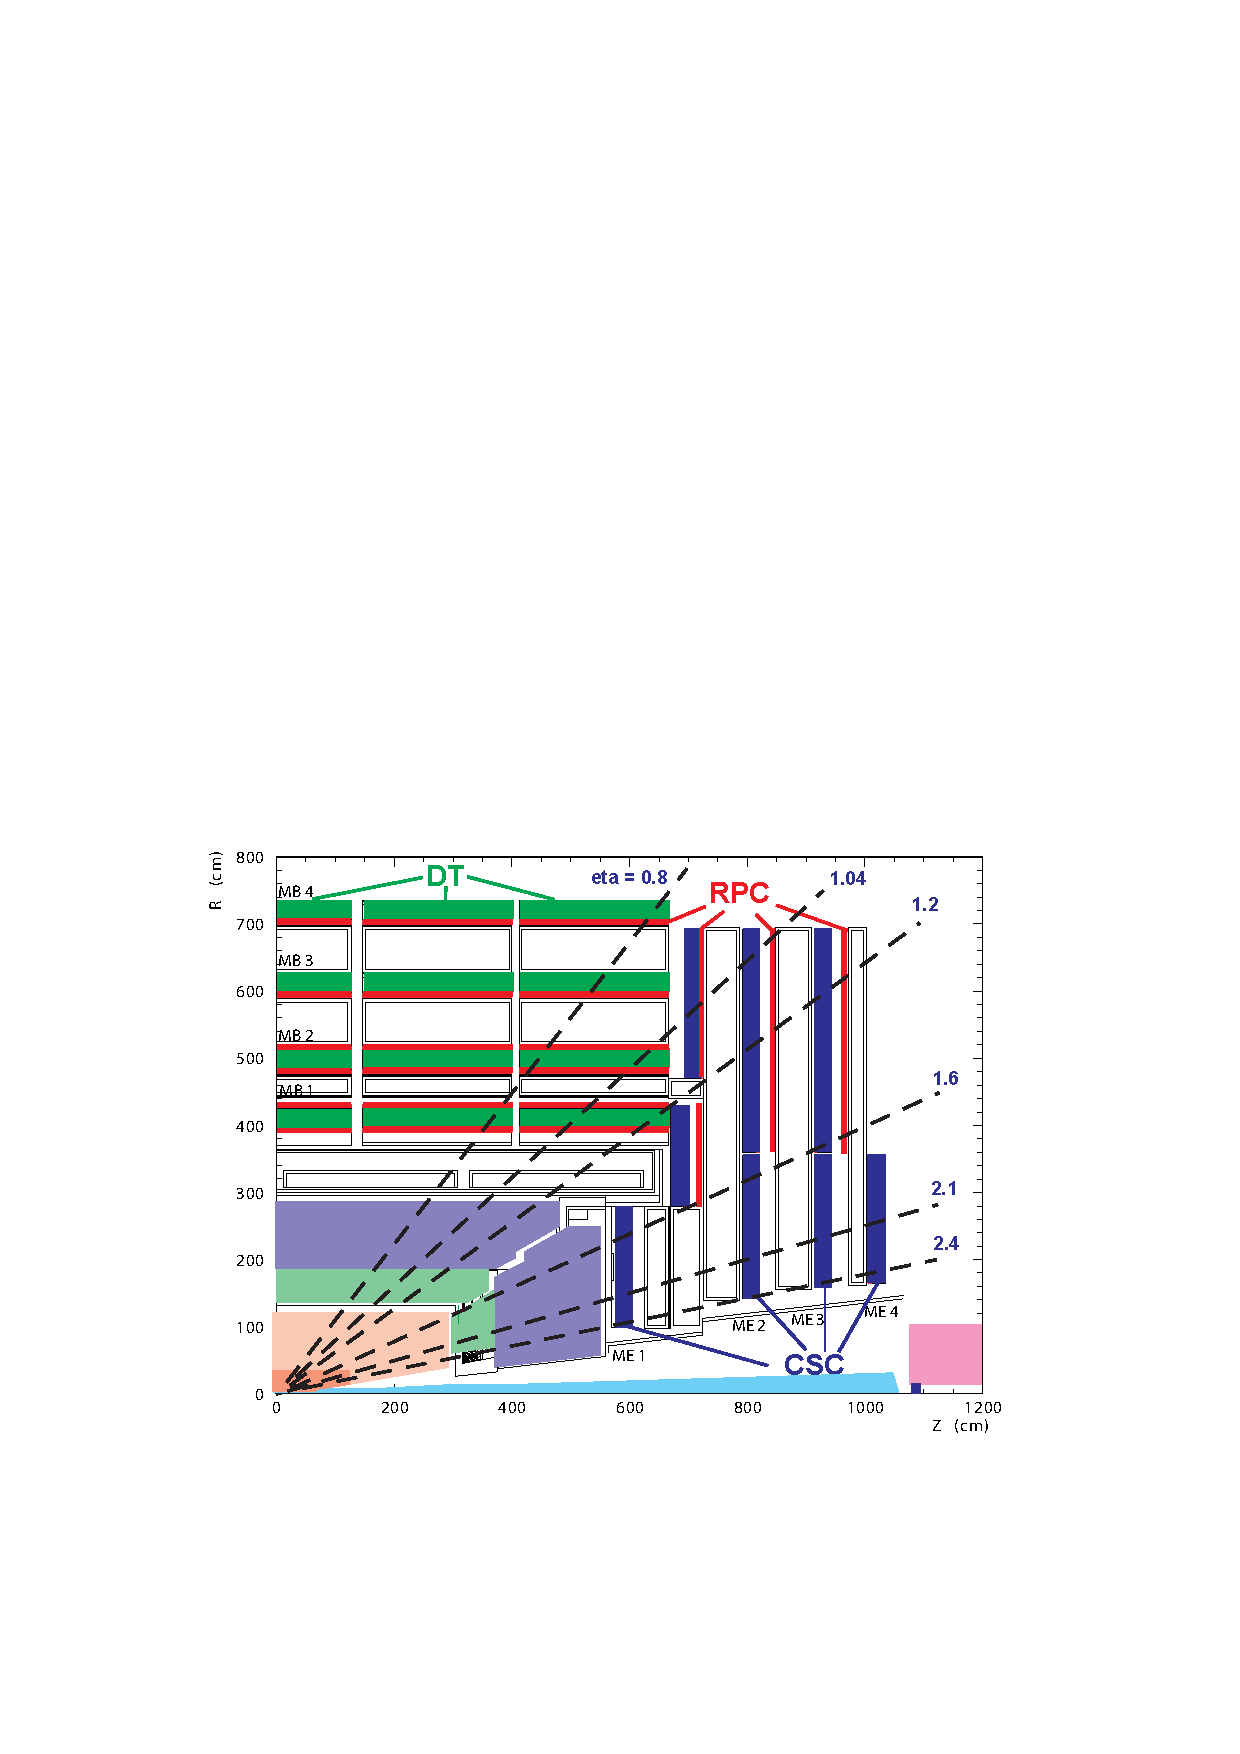
\includegraphics[width=\columnwidth]{muon_system}
    \caption{Layout of one quarter of the CMS muon system. Four drift tube (DT, in light orange) stations are labeled MB
    (“muon barrel”) and the cathode strip chambers (CSC, in green) are labeled ME (“muon endcap”). Resistive plate
    chambers (RPC, in blue) are in both the barrel and the endcaps of CMS, where they are labeled RB and RE,
    respectively.}
    \label{muon_system}
  \end{center}
\end{figure}

The layout of the CMS muon system is shown in Figure~\ref{muon_system}. It consists of the drift tubes (DT), cathode
strip chambers (CSC) and resistive plate chambers (RPC). The entire system surrounds the solenoid and covers the
pseudorapidity region of \abs\eta \num{<2.4}.

The drift tubes are located in the barrel region (\abs\eta \num{<1.2}). Consisting of four stations, they form
concentric cylinders around the beam line; there are \num{250} drift chambers with about \num{172000} sensitive wires in
total. When a muon passes through the volume, it knocks electrons off the atoms of the gas, which then follow the
electric field and reach the positively-charged wires, providing information on the muon's position. The chambers are
filled with the gas mixture of \SI{85}{\percent} $\textrm{Ar}$ and \SI{15}{\percent} $\textrm{CO}_2$, where the muon
drift time does not exceed \SI{380}{\ns}. Although this value is bigger than the typical bunch crossing time (\num{25}
or \SI{50}{\ns}), it is sufficient because of the small muon rate in this region.

In the endcaps, the cathode strip chambers cover the pseudorapidity region of \num{0.9} $<$\abs\eta\num{<2.4}. Each of
\num{468} CSCs is a trapezoidal multi-wire proportional chamber consisting of 6 gas gaps with a plane of radial cathode
strips and a plane of anode wires which are roughly perpendicular. A charged muon traversing each plane of a chamber
causes gas ionisation and a subsequent electron avalanche which produces a charge on the anode wire and an image charge
on the cathode strips. The gas used in CSCs is a mixture of $\textrm{Ar}$, $\textrm{CO}_2$ and $\textrm{CF}_4$.

The resistive plate chambers system is complementary to both DT and CSC systems, and is located in both barrel and
endcap regions (\abs\eta\num{<2.1}). RPCs also operate in avalanche mode with a gas mixture of C$_2$H$_2$F$_4$,
C$_4$H$_{10}$ and $\textrm{SF}_6$, and due to an excellent time resolution of about \SI{1}{\ns} they provide fast
information for triggering. The spacial resolution is, however, quite limited (\SI{\approx 1}{\cm}, compared to
\SI{\approx 100}{\micron} for DTs and CSCs). %http://arxiv.org/abs/1306.6905

\begin{figure}[htbp]
  \begin{center}
    \leavevmode
    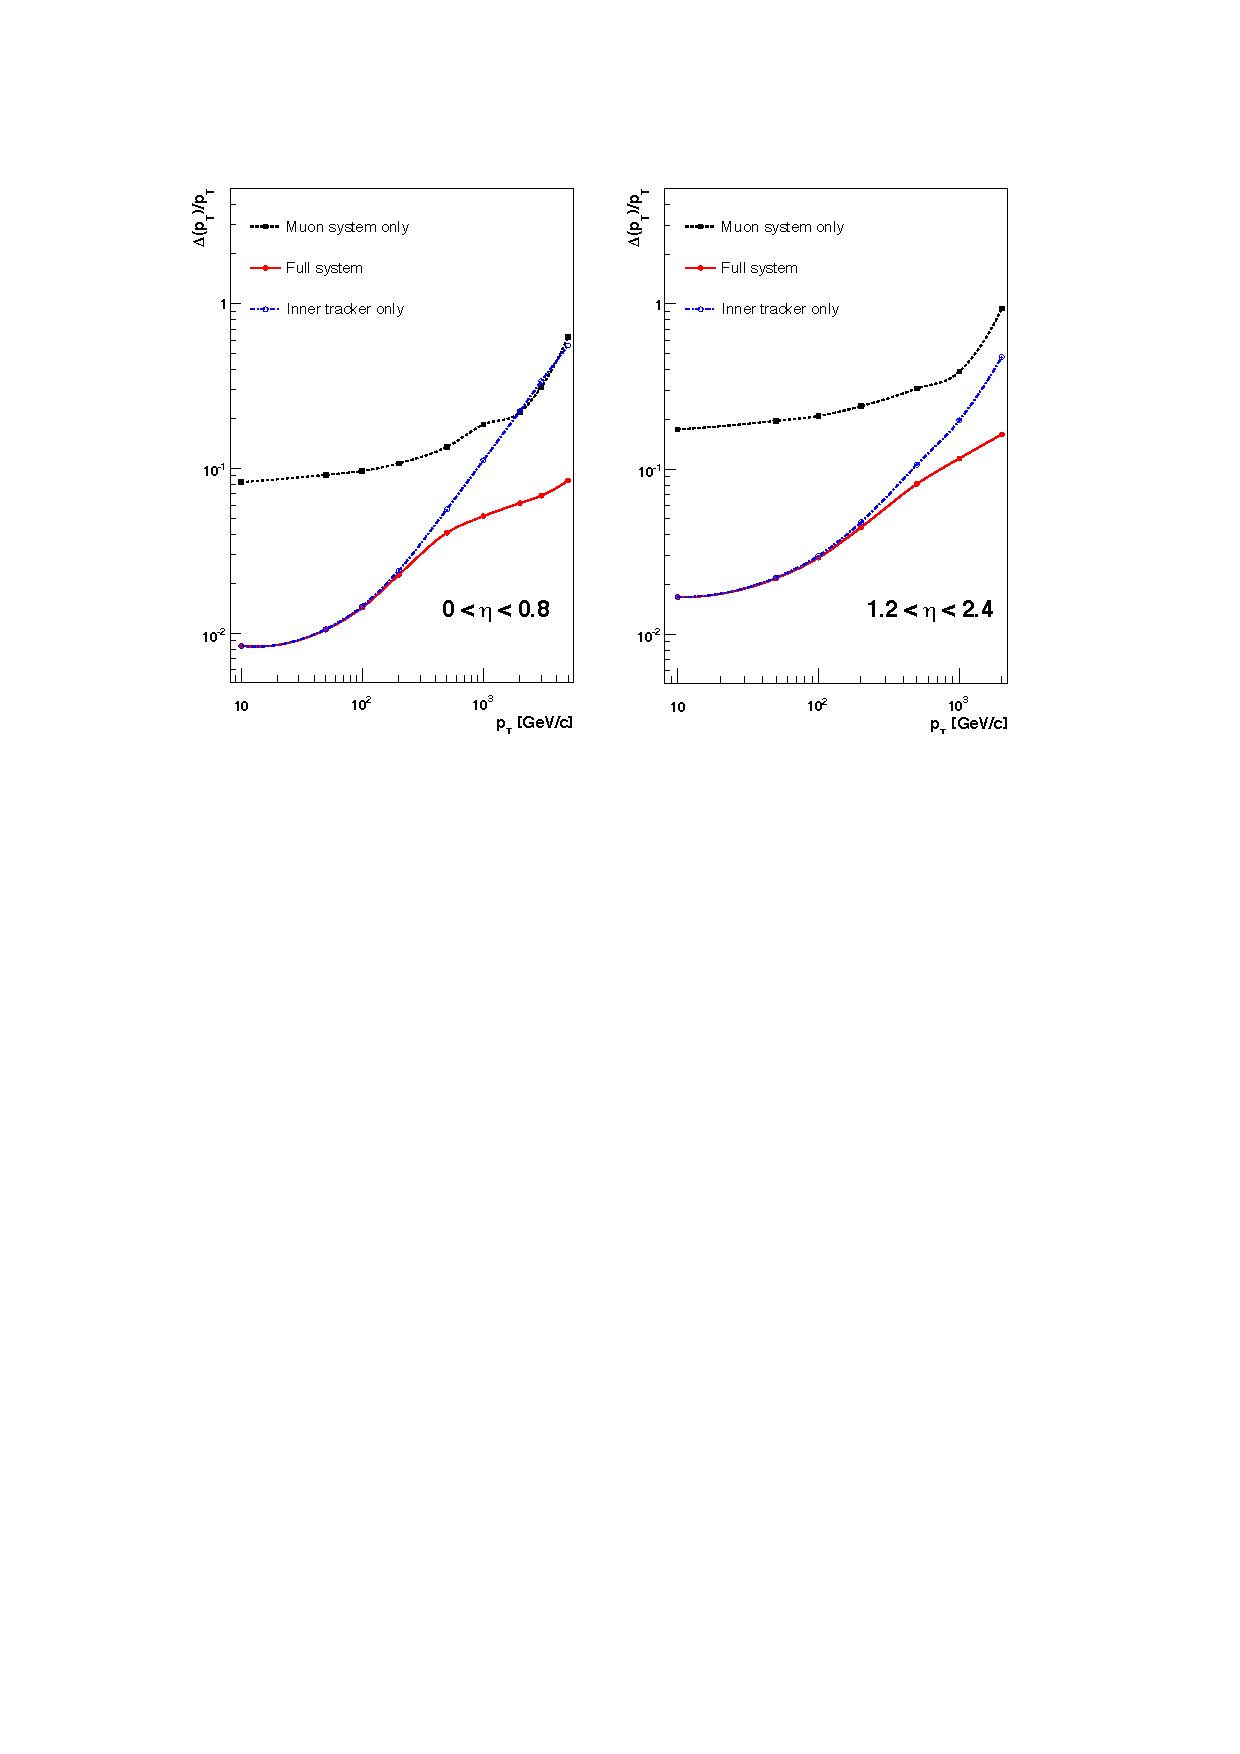
\includegraphics[width=\columnwidth]{muon_resolution}
    \caption{The muon transverse momentum resolution as a function of the transverse momentum (\pt) using the muon
    system only (black), the inner tracking only (blue), and both (red), in regions of \abs\eta \num{<0.8} (left) and
    \num{1.2} $<$\abs\eta\num{<2.4} (right) \autocite{CMS}.}
    \label{muon_resolution}
  \end{center}
\end{figure}

The muon momentum is measured in both the tracker and the muon system.  As it can be seen on
Figure~\ref{muon_resolution}, both sub-systems contribute to the momentum resolution at different \pt values. This
happens due to the difference in the magnetic field and detector technology. For low-\pt muons, the best momentum
resolution is obtained in the tracker, whereas in the high-\pt region the muon system provides a significant
improvement. Therefore, by using information from both the silicon tracker and the muon chambers (i.e.\ reconstructing
the ``global muon''), the momentum resolution is improved in the whole \pt region up to a \SI{\approx 1}{\TeV/c} level.

\subsection{Trigger and Data Acquisition}
\label{ss:trigger_daq}
At design LHC luminosity of $L = $ \SI{d34}{\cm^{-2} s^{-1}}, approximately \num{25} collisions are expected to occur at
each crossing of the proton bunches. The bunch spacing of \SI{25}{\ns} corresponds to a crossing rate of
\SI{40}{\mega\hertz}. Since every event produces \SI{\sim1}{\mega\byte} of raw data, it corresponds to a total data
production of \SI{40}{\tera\byte\per\second}. Attempting to store all of this data is clearly beyond the available
technology. Moreover, only a fraction of events contain hard scattering processes that are of interest, therefore an
effective trigger system had to be implemented.

The CMS trigger is a two-level system, consisting of two independent parts: the Level-1 (L1) trigger and the High-Level
Trigger (HLT). The L1 trigger is a hardware system implemented in programmable electronics residing partly on detector,
and partly in the underground control room located at approximately \SI{90}{\metre} from the experimental cavern. The
maximum latency between the collision and the L1 accept decision received by front-end electronics is
\SI{3.2}{\micro\second}. During this amount of time, the complete event information is buffered in pipelined memories
on the detector. The only information used for the L1 trigger decision is that from the muon system and the calorimetry.
Since the reconstruction of tracks exceeds the time scale required for the L1 decision, the tracker information can't be
used. The L1 trigger reduces the event rate from \SI{\sim40}{\mega\hertz} to \SI{\sim100}{\kilo\hertz}, corresponding to
a data flow of about \SI{100}{\giga\byte\per\second}. These events are fed into the HLT system.

The High-Level Trigger is a software system implemented in a single CPU farm, sometimes referred to as the ``Event
Filter Farm''. Having access to the full event information, customised algorithms of increasing complexity are used
which results in a highly flexible trigger system. The event rate is reduced down to \SI{\sim300}{\Hz}, with the final
data rate of approximately \SI{300}{\mega\byte\per\second} being stored on a large disk cache at the experimental site
(the Storage Manager) and later on transferred to CERN Tier 0 for further processing (see Section \ref{s:computing}).

Since the start of the LHC running, the operating conditions have been changing drastically. During the start-up year of
2010, the instantaneous luminosity went up from about \SI{d27}{\cm^{-2} s^{-1}} to approximately \SI{0.2d32}{\cm^{-2}
s^{-1}}. In 2011 the luminosity ramped up to a factor of \num{20} above that of 2010, reaching approximately
\SI{4d33}{\cm^{-2} s^{-1}}. This required a lot of continuous effort to control the trigger rates at reasonable level,
whilst also keeping its efficiency acceptable. In 2012 the luminosity was more stable, peaking at
\SI{\approx7.6d33}{\cm^{-2} s^{-1}} which is just a factor of 2 above the 2011 values. However, it still came as a
challenge because of the impact of pile-up. At a bunch spacing of \SI{50}{\ns} and increased centre-of-mass energy of
\SI{8}{\TeV}, the average number of pile-up vertices nearly doubled comparing to that in 2011, which required a major
CPU extension and implementation of sophisticated PU mitigation techniques at the HLT level. The author's contribution
to the HLT development of the trigger paths important for top physics is described in Chapter~\ref{c:service_work}.

\section{Computing}
\label{s:computing}
The vast amounts of data delivered by the CMS detector impose high requirements on the offline computing system. During
2010--2012 operation, CMS collected \SI{\sim10}{\peta\byte} of raw data per year. Including Monte Carlo simulations,
reconstructed data and analysis skims, the total annual amount of data essentially doubles. To handle the distributed
storage and processing of this data, not just for CMS but for the entire high energy physics community using the LHC, a
worldwide LHC computing grid (WLCG) has been put in place.

WLCG is a global collaboration of more than 150 computing centres in about 40 countries. The grid has a tiered
architecture, comprising 4 tiers with different resources and services. The first one, Tier 0, is based at CERN and is
responsible for data-taking. It accepts raw data from the data acquisition system and repacks it into primary datasets
according to the trigger information. The raw data is archived to tape, and is also prompt-reconstructed (within 48
hours) before being distributed to the Tier 1 (T1) centres around the world. There are 8 T1 sites based at large
national laboratories in collaborating countries (e.g.\ RAL in the UK and FNAL in the US). Each of the T1 centres is
used for large-scale centrally organised data-processing activities. The data is then distributed in the reduced format
(see Section~\ref{ss:edm}) to a more numerous set of Tier 2 centres, typically located at collaborating universities.
Each of these centres is used for the grid-based analysis and Monte Carlo simulation for the whole experiment, as well
as local services for groups maintaining them. The last stage of computing system, Tier 3, is meant solely for the local
institution's user analysis.

\subsection{Event Data Model}
\label{ss:edm}
In the basis of the CMS Event Data Model lies the concept of an event, which is physically a result of a single
collision in the LHC. From a software point of view, the event is a \Cplusplus object container storing raw data from a
single readout of detector electronics (e.g.\ hits in various sub-detectors), as well as reconstructed data which is
based on this information, such as tracks, clusters and physics objects. All these \Cplusplus objects are stored in ROOT
format \autocite{ROOT}.

The EDM makes use of three main data formats, based on different levels of detail and precision:
\begin{itemize}
  \item RAW format, containing full information from the detector as well as L1 and HLT trigger decisions, with the
  event size of \SI{\sim1.5}{\mega\byte}.
  \item RECO (reconstructed data) format, which is obtained from raw data by application of pattern recognition and
  compression algorithms. This data includes reconstructed detector hits, clusters and physics objects (electrons,
  muons, etc.). The typical event size is \SI{\sim250}{\kilo\byte}.
  \item AOD (Analysis Oriented Data) format, produced by filtering the RECO data from the reconstructed detector
  objects, leaving just the high-level physics objects required for analysis. The event size is reduced down to
  \SI{\sim50}{\kilo\byte}.
\end{itemize}

The RECO and AOD data are analysis-ready data formats, produced centrally and used by many physics analysis groups.
However, further simplification of the data is also a common practice. By transforming the \Cplusplus objects produced
by CMS software into plain basic types or vectors of them, only including the analysis-specific content, the event size
can be reduced down to \SI{\sim3}{\kilo\byte} level depending on the needs of a particular analysis. This data format is
often referred to as private ``ntuples'', and it requires specific analysis software capable of restructuring the data
into user-defined classes. By following this approach, the analysis can be run locally and generally much faster than
processing the RECO or AOD data. However, it requires ``ntuplising'' this data every time when new centrally-recommended
physics objects or corrections are produced.

\subsection{Analysis Software}
\label{ss:analysis_software}
Both of the analyses described in this thesis use the CMS software framework (CMSSW \autocite{CMSSW}), as well as
Bristol Analysis Tools (BAT \autocite{BAT}). The differential cross section analysis also uses an additional level of
python scripts for post-processing \autocite{DailyPythonScripts}.

CMSSW is the key CMS software framework built around the Event Data Model (see Section~\ref{ss:edm}). The framework is
essential for purposes of Monte Carlo simulation, detector calibration and alignment, as well as data reconstruction
and analysis. CMSSW has a modular architecture, consisting of one configurable executable (cmsRun) and a large set of
plug-in modules that contain all the code needed for event processing (reconstruction algorithms, calibration, etc.).
Different versions of CMSSW were used for different analyses: 

\begin{itemize}
  \item \verb!CMSSW_4_2_8! for the top mass analysis on 2011 data;
  \item \verb!CMSSW_4_4_4! for the missing transverse energy analysis on 2011 data;
  \item \verb!CMSSW_5_3_9! for the top cross pair cross section analysis on 2012 data.
\end{itemize}

Corresponding versions were used to produce ntuples for processing by BAT, which was used to read the data, apply
selections, calculate high-level variables and to create various histograms of distributions. BAT was originally started
in 2010 by Dr.\ Lukasz Kreczko for the needs of the Bristol top group, later on also developed by the author and other
researchers from Bristol and affiliated top groups. Like CMSSW, this framework has a modular structure, with its classes
falling in four main categories:

\begin{itemize}
  \item readers, for translating plain data types from ROOT files into \Cplusplus objects;
  \item RECO objects, i.e.\ output of the readers (physical objects like leptons, jets and its collections);
  \item selections, for application of event selections;
  \item analysers for creating histograms, applying selections, algorithms, and filling histograms.
\end{itemize}

All analysers are independent from each other, making the analysis chain stable and reliable. The final set of python
scripts is used to prepare the histograms, perform fitting and unfolding procedures (in case of cross section analysis),
and producing final tables and plots. Rootpy package \autocite{rootpy} was used to access ROOT libraries in python
interface, and matplotlib \autocite{matplotlib} was used to create plots.

\section{Object Reconstruction}
\label{s:object_reconstruction}
Most CMS analyses, including the ones described in this thesis, adopt a reconstruction technique called Particle Flow
(PF) \autocite{PF}. This algorithm is used to obtain a global event description at level of individually reconstructed
particles by means of combining information coming from all sub-detector systems. The ultimate goal is to determine
type, energy and momentum of all the particles in the event with highest possible precision and in the most optimal way.
The types of these particles include electrons, muons, charged hadrons, neutral hadrons and photons. All these particles
are then used to reconstruct jets (Section~\ref{ss:jet_reconstruction}), missing transverse energy
(Section~\ref{ss:electron_reconstruction}) and tau leptons from their decay products.

\subsection{Electron Reconstruction}
\label{ss:electron_reconstruction}
The reconstruction of the \ttbar pair with an electron in the final state imposes high requirements on the electron
identification and its energy-momentum measurement, precision of which is of major importance for both top mass and
\ttbar cross section measurements.

Although the CMS detector is equipped with highly accurate ECAL and tracker systems, electron identification and
reconstruction is still a challenging task due to the large amount of tracker material (see Section~\ref{ss:tracker}).
This results in a significant Bremsstrahlung photon emission, which often causes an ECAL energy deposit to be widely
spread in azimuthal direction because of the high magnetic field. Therefore, dedicated algorithms were developed in
order to collect all Bremsstrahlung energy deposits in the calorimeter (Bremsstrahlung recovery), and also to take into
account the kinks in the electron trajectory caused by photon emissions.

Electron reconstruction in CMS has following distinct stages: seeding, track finding, pre-identification, Bremsstrahlung
recovery, track-cluster linking and final identification. Historically, the original seeding algorithm was designed and
optimised for isolated high-\pt electrons. This approach starts from ECAL clusters, and therefore is called the
'ECAL-driven' seeding. It is based on the property of the ECAL energy deposits to have narrow width in the $\eta$
coordinate, and to be widely spread in $\phi$ (azimuthal direction) like it was mentioned above. The electron and all
the associated Bremsstrahlung energy deposits form a single ``super-cluster'', and the ability to correctly determine it
affects the overall performance of this method. Only super-clusters with transverse energy above \SI{4}{\GeV} are taken
into account. Super-clusters are then matched to pairs or triplets of hits in the inner tracker layers, forming the
track seeds on which the electron tracks are built upon.

The performance of the ECAL-driven method is not very well suited for non-isolated and low-\pt electrons. This occurs
mainly due to the fact that the super-cluster position and energy can be highly biased by the impact of overlapping
particles, especially if the electron happens to be within a jet and therefore non-isolated. Also, high track
multiplicity complicates the backward propagation from a super-cluster, because it can be consistent with a number of
track seeds corresponding to other particles. To minimise the number of these fake seeds, the ratio between the HCAL and
ECAL energy deposits ($H/E$) is required to be smaller than \num{0.15}. The HCAL towers used in the calculation of this
ratio are taken within a cone of $\DR = 0.3$ behind the super-cluster position. Although this helps to keep the fake
seed rate under control, the efficiency for non-isolated electrons becomes rather limited. As for the low-\pt electrons,
the wider azimuthal spread of Bremsstrahlung photons leads to poorer reconstruction of the super-cluster, biasing its
position and therefore preventing the efficient matching with a track seed.

Within the particle flow method, efficient reconstruction of non-isolated and low-\pt electrons is particularly
important since it affects the reconstruction of jets and missing transverse energy. Therefore, a different
('tracker-driven') seeding algorithm is used, which starts from reconstruction of tracks. The baseline of the CMS track
reconstruction is the Kalman filter (KF) \autocite{KF}, which is a linear least-squares estimator based solely on
Gaussian probability density functions. It is particularly suitable for muon reconstruction since it is dominated by
multiple Coulomb scattering and its impact is well modelled by Gaussian fluctuations. However, this approach usually
fails for electrons because Bremsstrahlung photon emission is highly non-Gaussian. To accommodate for the resulting
kinks in the electron trajectory, the Gaussian-Sum Filter (GSF) \autocite{GSF} is used, which is essentially a
non-linear generalisation of the Kalman Filter. In this method, Bremsstrahlung energy loss is modelled by a Gaussian
mixture, therefore GSF track fit provides a better estimate for the inner and outer track momentum comparing to the KF
algorithm. The downside of this approach is its high CPU usage, which means it can be run on a limited number of seeds.

The GSF tracks are reconstructed upon all ECAL-driven seeds. In case of the 'tracker-driven' seeds, a pre-identification
based on high-purity KF tracks has been adopted. This procedure starts with the tracks reconstructed with very tight
criteria, thus decreasing the fake rate yet compromising on tracking efficiency. Then an iterative-tracking strategy is
carried out by means of removing hits unambiguously assigned to tracks from the previous iteration, and also
progressively relaxing track seeding criteria. This approach leads to both high efficiency and low fake rate, which is
crucial for low-\pt and non-isolated electrons.

In the next step, track-cluster matching has to be performed. In case if electron has negligible Bremsstrahlung
emission, the track is well reconstructed with the KF algorithm all the way to the ECAL internal surface, where the
closest cluster is matched to the track. The corresponding cluster energy is compared with the track momentum, and if
the ratio ($E/p$) is close to unity, the track is selected. On the contrary, if the electron experiences a significant
Bremsstrahlung emission, other track characteristics have to be exploited. In this case a selection based on the number
of hits in the tracker and the $\chi^2_\textrm{KF}$ of the KF fit is applied before running a GSF refit. Finally, the
number of hits, the GSF refit $\chi^2_\textrm{GSF}$, $\chi^2_\textrm{KF}/\chi^2_\textrm{GSF}$ ratio, the energy loss
measured by the track and the quality of the ECAL cluster-track matching are fed into a multivariate analysis using a
Boosted Decision Trees (BDT) estimator.

Both tracker-driven and ECAL-driven seeds are used to obtain the GSF track collection of electron candidates. In the
particle flow algorithm, it is necessary to link both electron and Bremsstrahlung energy deposits to the GSF track. A
super-cluster is linked to a track if the extrapolated position from the outermost tracker measurement is within the
boundaries of one of the ECAL cells at the expected depth of the electron shower maximum. The preshower-ECAL and
ECAL-HCAL links are made in a similar way.

Another important particle flow procedure, also driven by GSF tracks, is Bremsstrahlung recovery. In order to
reconstruct an electron with correctly assigned energy and momentum, it is crucial to identify all energy deposits from
Bremsstrahlung photons, thus forming a super-cluster. This procedure is carried out for each tracker layer by computing
a straight-line extrapolation tangent to the track, up to the calorimeter. To determine a Bremsstrahlung photon,
track-cluster linking is performed as described above. To limit the charged hadron contamination, clusters already
assigned to KF tracks are not included in the calculation. Also, the distance in $\eta$ coordinate between the
extrapolation and the cluster is required to be smaller than \num{0.015}, which helps to reduce the neutral particles
background.

\subsubsection{Electron Identification}
\label{sss:electron_id}

Electron reconstruction in CMS is based on a characteristic signature that electrons leave in the tracker and
calorimetry systems. However, other objects like charged hadrons, jets or photon conversions can produce very similar
signatures and therefore may be reconstructed as electrons. Therefore, in order to distinguish these ``fake'' electrons
from ``real'' ones, a further selection has to be applied. This procedure is referred to as electron identification (or
electron ID).

Initially the electron identification is performed at the final stage of the electron reconstruction process. The
working points of the cuts applied are selected to be loose enough in order to satisfy most CMS analyses requirements.
Afterwards, more specific (tighter) ID cuts are applied for each individual analysis, defining the working point in the
trade-off between selection efficiency and fakes contamination. This will be discussed separately in the selection
description for each analysis in corresponding chapters.

There are several electron identification algorithms used by various CMS analyses, and four of them are used in the
analyses described in this thesis: simple cut-based (SCB ID), cuts in categories (CiC ID), particle flow (PF ID) and
multi-variate analysis (MVA ID).

Simple cut-based identification is used in the High-Level Trigger, and therefore has to be as simple, fast and
robust as possible. Cuts are applied on the following variables:

\begin{itemize}
  \item $H/E$, i.e.\ the ratio of hadronic energy of the HCAL towers centred at the super-cluster position of the
  electron in a cone of radius $\Delta R = 0.15$, and the super-cluster electromagnetic energy;
  \item $\Delta\eta_{\text{in}}$, i.e.\ the difference in $\eta$ between the extrapolated track position and $\eta$ of
  the super-cluster;
  \item $\Delta\phi_{\text{in}}$, i.e.\ the difference in $\phi$ between the extrapolated track position and $\phi$ of
  the super-cluster;
  \item $\sigma_{i\eta, i\eta}$, i.e.\ cluster shape of the electron energy in a $5\times5$ block of crystals around the
  seed crystal (the one with the highest energy) \autocite{electron_reconstruction}:
  \begin{equation}
  \label{eq:cluster_shape}
    \sigma_{i\eta, i\eta} = \sum_{5\times5 \text{ crystals}} \left(\eta_i - \eta_\text{seed cluster}\right)^2
    \frac{E_i}{E_{\text{seed cluster}}}
  \end{equation}
\end{itemize}

Although this identification method has an advantage of its simplicity, it does not show the best signal efficiency and
background rejection. One of the more complex methods is the CiC ID, which exploits the categorisation of electrons. It
is optimised to select electrons from different sources (W, Z and J/$\psi$ decays) and reject fakes from jets or
conversions. In order to achieve higher efficiency, electron candidates are split into categories with different signal
to background ratio, allowing to better tune the working points of the cuts. The first step in categorisation is done by
division between barrel and endcap regions of the detector. Since the properties of both the tracker and calorimetry
systems differ significantly in these two regions, different cuts are applied. The second step is based on the following
observables:

\begin{itemize}
  \item $f_\text{brem}$, or measured bremsstrahlung fraction, defined as:
  \begin{equation}
  \label{eq:fbrem}
    f_\text{brem} = \frac{p_\text{in}-p_\text{out}}{p_\text{in}}
  \end{equation}
  where $p_\text{in}$ is the initial track momentum at the vertex and $p_\text{out}$ is the track momentum at the last
  hit;
  \item $E/p$, which is the ratio of the super-cluster energy and the initial track momentum.
\end{itemize}

Three categories of electron candidates are distinguished \autocite{CiC_ID}:
\begin{itemize}
  \item ``Low-Brem'': $0.9 < E/p < 1.2 - f_\text{brem} < 0.12$ (barrel), $0.82 < E/p < 1.22 - f_\text{brem} < 0.2$
  (endcap), the fake-like region with high number of both real and fake electrons;
  \item ``Bremming'': $0.9 < E/p < 1.2 - f_\text{brem} > 0.12$ (barrel), $0.82 < E/p < 1.22 - f_\text{brem} > 0.2$
  (endcap), the electrons-like region with a little contamination from fakes;
  \item ``Bad-Track'': remaining regions with a low number of real electrons.
\end{itemize}

The third and the final step in categorisation is based simply on the electron transverse energy, with the lower
threshold taken as \SI{10}{\GeV}. In each category, the selection is performed on the basic ID variables already
mentioned above for the simple cut-based identification. On top of these variables, isolation and conversion rejection
variables are also used, they are discussed in Section~\ref{sss:electron_isolation} and
Section~\ref{sss:photon_conversions}, respectively.

The cuts within CiC ID are applied in order to maximise the signal to background ratio. Depending on the needs of
different analyses, nine levels of cut severity are implemented: \textit{VeryLoose, Loose, Medium, Tight, SuperTight,
HyperTight(1-4)}. Each step decreases the fake rate by about a factor of two for electrons with \ET$>$ \SI{20}{\GeV}
\autocite{CiC_ID}. The CiC ID is used as a primary electron identification method in the Top Mass analysis
(Chapter~\ref{c:top_mass_analysis}).

Particle flow ID is the final step of the particle flow electron reconstruction. Following the particle flow concept,
is uses information from all the CMS sub-detectors obtained in previous reconstruction steps to build new observables
for electron identification. The complete list of PF ID observables is given below:
\begin{itemize}
  \item \pt and $\eta$ of the GSF track;
  \item GSF $\sigma_{p_\text{T}}/p_\text{T}$, transverse momentum resolution of the GSF track;
  \item \#hits$_\text{KF}$, number of reconstructed KF track hits;
  \item $\chi^2_\textrm{GSF}$ and $\chi^2_\textrm{KF}$, GSF and KF goodness-of-fits;
  \item $\Delta\eta$: distance in $\eta$ between the position of the cluster and the extrapolated position of the
  GSF track;
  \item $\sigma_{\eta\eta}$, cluster shape (Equation~\ref{eq:cluster_shape}) of the ECAL cluster linked to the
  GSF track;
  \item $H/(H+E_\text{e})$, hadron fraction of the shower, where $H$ is the energy of the hadron cluster linked to
  the GSF track;
  \item $(E_\text{e}+\sum E_\gamma)/p_\text{in}$, ratio between the super-cluster energy and the inner track
  momentum;
  \item $E_\text{e}/p_\text{out}$, ratio between the electron cluster energy and the track outer-momentum;
  \item $\sum E_\gamma/(p_\text{in}-p_\text{out})$, the ratio between the Bremsstrahlung photon energy as measured by
  ECAL and by the tracker;
  \item $EarlyBrem$, flag of $(E_\text{e}+\sum E_\gamma)>p_\text{in}$ inequality, corresponding to an electron
  emitting an ``early'' Bremsstrahlung photon, i.e.\ before it has crossed at least three tracker layers;
  \item $LateBrem$, flag of $E_\text{e}>p_\text{out}$ inequality, corresponding to an electron emitting a ``late''
  Bremsstrahlung electron, when the ECAL clustering is not able to disentangle the overlapping electron and photon
  showers;
  \item $f_\text{brem} = (p_\text{in}-p_\text{out})/p_\text{in}$, Bremsstrahlung fraction (Equation~\ref{eq:fbrem}).
\end{itemize}

All these variables are combined into a single discriminator by a multivariate analysis technique (BDT method), which
has been trained on signal and background Monte Carlo samples. PF ID is a relatively loose identification method, since
it has to satisfy the needs of all analyses using particle flow collections.

Finally, MVA electron identification is used in top cross sections analysis on 2012 data. It is another multivariate
analysis technique, optimised to select isolated electrons from W and Z decays. The variables used in MVA ID are also
combined into a single discriminator, they are largely similar to the ones used in PF ID:

\begin{itemize}
  \item \pt and $\eta$ of the GSF track;
  \item \#hits$_\text{KF}$, number of reconstructed KF track hits;
  \item $\chi^2_\textrm{GSF}$ and $\chi^2_\textrm{KF}$, GSF and KF goodness-of-fits;
  \item $\Delta\eta$: distance in $\eta$ between the position of the cluster and the extrapolated position of the
  GSF track;
  \item $\Delta\phi$: distance in $\phi$ between the position of the cluster and the extrapolated position of the
  track;
  \item $\Delta\eta_{vtx}$: distance in $\eta$ between the position of the cluster and the position of the GSF track
  at vertex;
  \item $\Delta\phi_{vtx}$: distance in $\phi$ between the position of the cluster and the position of the GSF track
  at vertex;
  \item $\sigma_{\eta \eta}$, cluster shape in $\eta$;
  \item $\sigma_{\phi \phi}$, cluster shape in $\phi$;
  \item $\eta$ width of the super-cluster;
  \item $\phi$ width of the super-cluster;
  \item $H/E$, ratio of HCAL and ECAL cluster energy;
  \item $E_\text{super-cluster}/p_\text{T}$, ratio between the super-cluster energy and the track momentum;
  \item $1/E_\text{super-cluster} - 1/p_\text{T}$, difference between inverse super-cluster energy and inverse
  track momentum;
  \item $E_\text{e}/p_\text{out}$, ratio between the electron cluster energy and the track outer-momentum;
  \item $1-E_{1\times 5}/E_{5\times 5}$, where $E_{1\times 5}$ is the energy in the central $1\times 5$ strip of the
  $5\times 5$ electron cluster and $E_{5\times 5}$ its total energy;
  \item $E_{3\times 3}/E_\text{super-cluster, raw}$, ratio of the energy of a cluster of $3\times 3$ and the
  uncorrected (raw) energy of the super-cluster;
  \item $E_\text{PS}/E_\text{super-cluster, raw}$, ratio of the energy in the preshower detector and the raw
  super-cluster energy (only in the endcap region).
  % Surely there are isolation variables? There's no MVA documentation whatsoever. Absolute joke.
\end{itemize}

\subsubsection{Electron Isolation}
\label{sss:electron_isolation}

Isolation is an observable that allows to distinguish prompt electrons (i.e.\ the ones from W and Z decays) from jets
faking electrons and electrons within jets. It is essentially a measure of activity around the particle. In CMS, there
are two different ways of quantifying isolation: detector-based and particle-based. The detector-based isolation is
defined separately for each detector sub-system (tracker, ECAL and HCAL):

\begin{itemize}
  \item Tracker isolation, calculated as the sum of transverse momenta of all track within a cone of $\Delta R = 0.3$
  around the electron, excluding the electron momentum itself;
  \item ECAL isolation, i.e.\ the sum of transverse energy of all ECAL clusters within a cone of $\Delta R = 0.3$
  around the super-cluster position. The footprint of the original electron is also removed;
  \item HCAL isolation, defined as the sum of transverse energy of all HCAL towers within a cone of $\Delta R = 0.3$
  centred at the super-cluster position.
\end{itemize}

Particle-based isolation exploits the particle flow information: it is calculated as the sum of transverse energy of all
PF particles in the cone of $\Delta R = 0.3$ around the electron. Both detector-based and particle-based isolation
definitions are often normalised to the electron transverse momentum (or energy in case of calorimeter isolation) in
order to improve signal efficiency. The normalised sum of the tracker, ECAL and HCAL isolation variables is referred to
as detector-based relative isolation (or \reliso), similarly normalised particle-based isolation is called PF \reliso.
These quantities are crucial in various methods to estimate the QCD background contribution for many analyses, and will
be used for both electrons and muons throughout this thesis.

\subsubsection{Identification of photon conversions}
\label{sss:photon_conversions}
Interacting with detector material, photons can convert into electron-positron pairs. Due to the large amount of
material budget in the tracker (Figure~\ref{tracker_material_budget}), especially in the endcap region, there is a high
chance of conversions to happen. The resulting electrons can successfully fake prompt signal electrons, passing all the
identification criteria and appearing isolated if the initial photon was isolated, too. Therefore conversions constitute
a large proportion of the QCD background to top signal. The electron-positron pair may not be symmetrical in transverse
momenta, therefore a veto on a second electron is not sufficient to reject such electrons and other conversion
identification criteria are necessary.

The simplest method is based on counting the number of missing hits in the tracker. Conversions are most likely to
happen at some distance from the interaction point, essentially anywhere between the point of photon production and the
end of the tracker. Therefore electrons produced in such conversions are likely not to traverse through all the pixel
layers. To separate these electrons from the prompt ones, a cut on the number of missing layers can be used. However,
this approach fails if conversion occurs in the beam pipe, or if the reconstructed electron track is paired with
unrelated hits in the tracker, making it look like a prompt electron.

A slightly more sophisticated method is a partner track method. It is based on geometrical cuts on $dist$ and $dcot$
variables, which refer to the distances between tangent points of any two tracks in the $r-\phi$-plane and $r-z$-plane,
respectively:
\begin{equation}
  dist = \left|\left|\vec{r}_1 - \vec{r}_2 \right|- r_1 - r_2\right|
\end{equation}
\begin{equation}
  dcot = \left|\frac{1}{\tan\theta_1} -\frac{1}{\tan\theta_2}\right|
\end{equation}
Here $\vec{r}_{1,2}$ are radial vectors of the two tracks, $r_{1,2}$ are the track radii and $\theta_{1,2}$ -- angles
between the tracks and the beam pipe. Apart from the cuts on $dist$ and $dcot$ variables, tracks should have opposite
charge in order to be considered to come from a photon conversion.

These two methods for conversion identification were used in the top mass analysis on 2011 data. For the top cross
sections analysis on 2012 data, along with the number of hits method, a more advanced technique called vertex fit was
used. It is essentially a full vertex fit of all pairs of tracks, with the selection being made on the the fit
probability. The method benefits from the full use of track uncertainties and covariances, combining all information
into a single discriminator. However, increased complexity of this technique makes it more CPU-intensive than the
partner track method.

% internal source: https://twiki.cern.ch/twiki/bin/view/CMS/ConversionTools

\subsection{Muon Reconstruction}
\label{ss:muon_reconstruction}
A good muon reconstruction and identification was one of the main CMS design requirements. Initially, muons are
reconstructed independently in the tracker (``tracker tracks'') and in the muon system (``standalone muon tracks'')
using the Kalman Filter technique \autocite{KF}. Based on these objects, two different reconstruction methods are used:
\autocite{muon_reconstruction}

\begin{itemize}
  \item Global muon reconstruction. Each standalone muon track reconstructed in the muon system is matched with the
  tracker track by propagating onto a common surface. A global fit is performed on the combined collection of hits from
  both tracks, and the resulting muon is referred to as a \textit{global muon}.
  \item Tracker muon reconstruction. All tracker tracks above certain threshold (\pt $>$ \SI{0.5}{\GeV}, $p >$
  \SI{0.5}{\GeV}) are extrapolated to the muon system, taking into account possible energy losses, magnetic field and
  multiple Coulomb scattering. If the track matches at least one muon segment in the muon system, i.e.\ a short track
  stub made of DT or CSC hits, it is considered a \textit{tracker muon}.
\end{itemize}

Global muon reconstruction has a high efficiency for high-\pt muons, penetrating through more than one muon station. On
the contrary, tracker muon reconstruction is more efficient for low-\pt muons (\pt $<$ \SI{5}{\GeV}), as it requires
just a single muon segment. Since the \ttbar analyses described in this thesis have a semileptonic signature with
exactly one energetic muon in the final state (in case of the muon channel), only the global muon reconstruction method
is used, as its momentum resolution at high transverse momenta benefits from both the tracker and the muon system
(Figure~\ref{muon_resolution}).

Following the reconstruction, the quality of the muon objects is verified by applying identification criteria. This is
done in order to suppress hadronic punch-through, muons from decays in flight and cosmic muons. Selection is applied on
the following observables:
\begin{itemize}
  \item normalised $\chi^2$ ($\chi^2$/number of degrees of freedom) of the global muon fit;
  \item number of muon chamber hits in the global muon fit;
  \item number of muon stations with muon segments;
  \item transverse impact parameter $d_{xy}$ (closest approach of the track to the primary vertex);
  \item longitudinal distance $d_z$ of the tracker track w.r.t. the primary vertex;
  \item number of hits in the pixel detector;
  \item number of hits in the tracker layers.
\end{itemize}

The muon identification also exploits the CMS particle flow event reconstruction, making use of information coming from
all sub-detectors. Particle flow muons (PF muons) are identified by imposing selection on all muon candidates
reconstructed with the global muon method. This selection was optimised for identification of muons in jets, minimising
the fake rate from misidentified charged hadrons, which is crucial for correct reconstruction of jets and missing
transverse energy (described in more detail in the following sections). Depending on the analysis specifics, isolation
requirements can also be applied; isolation definitions closely follow the ones for electrons
(Section~\ref{sss:electron_isolation}).

%internal source https://twiki.cern.ch/twiki/bin/view/CMSPublic/SWGuideMuonId

\subsection{Jet Reconstruction}
\label{ss:jet_reconstruction}
Hadronisation of quarks and gluons leads to production of narrow cones of particles moving in approximately one
direction, called jets. This happens due to colour confinement, as particles carrying a colour charge cannot exist in
free form, they have to fragment into hadrons before they can be detected directly. Therefore, to measure the initial
parton's momentum and energy, all these particles must be combined into jets.

The CMS particle flow algorithm implies reconstruction of individual particles (charged and neutral hadrons, electrons,
muons, photons) before combining (or clustering) them into jets. A few different jet clustering techniques exist, but
the one used predominantly in CMS and exclusively in this work is \antikt algorithm \autocite{anti-kt}, which defines
the distance between constituent particles as:
\begin{equation}
d_{ij} = \min\left(\frac{1}{k^2_{t,i}},\frac{1}{k^2_{t,j}}\right) \frac{\Delta_{i,j}^2}{R^2}
\end{equation}
where $\Delta_{i,j}^2 = (y_i-y_j)^2 + (\phi_i-\phi_j)^2$, $k_{t,i/j}$, $y_{i/j}$ and $\phi_{i/j}$ are respectively
transverse momenta, rapidities and azimuth angles of particles $i/j$, and $R$ is the radius parameter.

The clustering proceeds by identifying the smallest distances between particles and recombining them until all jets are
formed and no particles are left. An event typically has a few well-separated hard (high-\pt) particles and a large
amount of soft (low-\pt) particles. The distance $d_{1i}$ between a hard particle 1 and a soft particle $i$ will be
fully determined by the transverse momentum of the hard particle and the $\Delta_{1i}$ separation. On the other hand,
distance between soft particles with similar separation will be substantially larger. Therefore, soft particles tend to
cluster around the hard ones before they cluster amongst themselves. On the output, the \antikt algorithm forms
conical jets with boundaries resilient to soft radiation.

\subsubsection{Jet Energy Corrections}
\label{sss:JEC}

Due to non-linear and non-uniform response of the calorimetry systems, jets reconstructed using detector inputs
typically have energies different to the ones of corresponding Monte Carlo particle jets (or generator jets),
reconstructed by clustering the four-momenta of all stable particles generated in Monte Carlo simulation. Therefore some
mapping procedure is necessary. Corrections applied to  reconstructed jets in order to translate the measured energy to
the true particle (or parton) energy are referred to as jet energy corrections, or JEC.

CMS has adopted a factorised approach of applying jet energy corrections, meaning that each correction level takes care
of a different effect. The set of corrections is applied sequentially, i.e.\ the output of each step is the input to the
next one. Essentially, each level of correction is a scaling of a jet four-momentum, with a scale factor depending on
various parameters of the jet, typically pseudorapidity and transverse momentum. Currently, the correction levels go as
follows:

\begin{itemize}
  \item L1 Offset correction;
  \item L2 Relative ($\eta$) correction;
  \item L3 Absolute (\pt) correction;
  \item L4 EMF (electromagnetic energy fraction) correction;
  \item L5 Flavour correction;
  \item L6 UE (underlying event) correction;
  \item L7 Parton correction.
\end{itemize}

The goal of the L1 correction is subtraction of pile-up and electronic noise contributions from the jet energy. The
energy from pile-up vertices can be deposited in calorimeters since the additional proton-proton collisions occur close
enough in time to the hard scattering process. Electronic noise in calorimeter readouts also creates additional energy
offset which needs to be corrected for. The scale factors for L1 correction are derived using data-driven methods
(zero-bias collisions).

The relative L2 correction is designed to flatten the jet response in pseudorapidity. These corrections are extracted
with respect to the barrel region in bins of \pt, and therefore are uncorrelated with the following L3 corrections. Both
Monte Carlo and data-driven (dijet balance) methods are used to derive the L2 scale factors. Once a jet is corrected for
$\eta$ dependence, it is corrected back to the particle level by applying absolute L3 correction. The goal of this
correction is to flatten the jet response in transverse momentum. Derivation of L3 scale factors is done by using Monte
Carlo truth information, or data-driven $Z/\gamma$+jet balance techniques.

The L4 EMF correction takes care of variations in jet response with respect to electromagnetic energy fraction, i.e.\
the fraction of energy deposited in ECAL by hadrons. Although it has been shown that EMF-dependent correction in three
parameters (\pt, $\eta$, EMF) can improve the observed jet resolution, this correction is optional for most CMS analyses
and hasn't been used in this work.

Another optional correction is the L5 flavour correction, which is intended to correct the jets depending on the flavour
of initiating partons, i.e.\ light quarks, heavy ($b$ and $c$ quarks), or gluons. Jets originating from heavy quarks are
different from light quark jets in a few aspects. The average number of charged hadrons within $b$-jets is higher than
the one for the light jets, although the average momentum of charge hadrons is smaller. Moreover, $b$-hadrons have a
larger branching fraction into semileptonic decays with neutrinos in the final state that cannot be detected. All these
factors may lead to a substantially smaller charged hadron energy fraction comparing to the light jets, therefore the
average calorimeter energy response is lower for the $b$-jets. These effects are meant to be taken care of by the L5
correction, which is derived either from Monte Carlo or data-driven \ttbar events.

Underlying event \autocite{underlying_event} refers to all the activity in the proton-proton collision apart from the
process of interest, i.e.\ the hard scattering process. It includes particles coming from additional parton interactions
(or multiple scatterings) and beam remnants. Depending on the analysis goals, underlying event may also include initial
and final state radiation (ISR and FSR) which represent the soft gluon radiation before and after the hard scattering
process, respectively. Underlying event activity results in production of additional soft jets which can bias the jet
energy measurement. Optional L6 UE correction attempts to mitigate such bias. However, it was not used in the analyses
described in this thesis, since underlying event is an intrinsic part of proton-proton interactions effectively modelled
by Monte Carlo simulation. In particular, the top cross sections analysis is designed to be very sensitive to such
higher-order processes, and not taking them into account may result in compromising the discriminating power between
Monte Carlo generators.

Finally, L7 parton correction attempts to correct the jet energies back to the parton level. It is also optional and was
only used in the top mass analysis. The correction factors were derived from Monte Carlo simulations by comparing the
generator jets momenta to their matched partons.

Due to the fact that CMS simulation is not perfectly tuned to the data yet, additional residual L2L3 corrections are
applied in order to achieve better agreement between data and simulation. It is essentially a small residual $\eta$- and
\pt-dependent calibration applied exclusively to data, which will remain in place until CMS develops a perfectly tuned
simulation reproducing the data features out of the box.

%internal source: https://twiki.cern.ch/twiki/bin/view/CMS/IntroToJEC

%Jet energy resolution? https://twiki.cern.ch/twiki/bin/view/CMS/JetResolution

\subsubsection{Particle Flow Jet Identification}
\label{sss:PFJet_ID}
To ensure the quality of the jets, a final identification criteria are applied to all jet objects. Particle flow jet
identification (or PF jet ID) is used to reduce the noise and rate of electrons reconstructed as jets. The cuts are
applied on the following observables :

\begin{itemize}
  \item number of constituent particles;
  \item NHF (neutral hadron energy fraction);
  \item CHF (charged hadron energy fraction);
  \item NEF (neutral electromagnetic energy fraction);
  \item CEF (charged electromagnetic energy fraction).
\end{itemize}

A rather loose identification cuts (referred to as ``loose PF jet ID'') were used in this work: a requirement of more
than one constituent particle in the jet, NHF$<0.99$, CHF$<0.99$, NEF$>0$ and CEF$>0$ in pseudorapidity region of
$\eta<2.4$.

\subsubsection{b-tagging}
\label{sss:b-tagging}
The identification of jets originating from b-quarks, or b-tagging, is one of the  most important tools in top quark
physics, capable of significantly decreasing the background contamination of signal processes. A variety of b-tagging
algorithms have been developed by CMS \autocite{b-tagging_CMS}, and the one that was used in this work is called
combined secondary vertex (CSV) algorithm. It is based on the fact that b-hadrons have a significant lifetime (\SI{\sim
e-12}{s}) and can travel a distance of a few centimetres before decaying. Therefore jets originating from b-quarks are
likely to have a secondary vertex located at a considerable distance from the primary vertex, which can be used as an
efficient discriminator between light jets and b-jets. In order to maximise its efficiency, apart from the secondary
vertex information the CSV algorithm also exploits the track-based lifetime information. The following variables are
used in the algorithm:
\begin{itemize}
 \item number of tracks in the jet;
 \item number of tracks at the secondary vertex;
 \item secondary vertex category;
 \item secondary vertex invariant mass;
 \item ratio of the total track energy at secondary vertex with respect to all tracks in the jet;
 \item pseudorapidities of tracks at secondary vertex with respect to the jet axis;
 \item impact parameter significance (i.e.\ ratio of IP to its uncertainty) of the first track that increases the
 invariant mass above the charm threshold of \SI{1.5}{\GeV} (tracks are ordered by IP significance; the mass of the
 system is recalculated after adding each track);
 \item impact parameter significances of each track in the jet.
\end{itemize}

All these observables are combined into a single discriminator, the ``medium'' working point of which is used in this
work. It provides \SI{\sim70}{\percent} b-tagging efficiency for mis-tag rate of approximately \SI{1}{\percent}
\autocite{b-tagging_CMS}.

\subsection{Missing Transverse Energy}
\label{ss:MET_reconstruction}
Due to the energy and momentum conservation, the sum of transverse momenta and energy of all particles in the final
state of proton-proton collisions is expected to be zero. However, some particles can escape the detector without being
reconstructed, therefore creating the imbalance in transverse momentum which is referred to as missing transverse
energy, defined as:
\begin{equation}
\label{eq:MET}
\vec{E}_\mathrm{T}^\mathrm{miss} = - \sum_i \vec{p^i}_\mathrm{T}
\end{equation}
where $\vec{p^i}_\mathrm{T}$ are the transverse momentum vectors of all reconstructed particles. The modulus of
$\vec{E}_\mathrm{T}^\mathrm{miss}$ vector is denoted by \MET.

Accurate reconstruction of missing transverse energy is crucial for precise measurements of Standard Model processes
with neutrinos in the final state. Top quark pair semileptonic decay is one of such processes, therefore analyses
covered in this thesis implicitly (top mass) or explicitly (\ttbar cross section with respect to \MET-related variables)
rely on efficient reconstruction of \MET. Misidentification and misreconstruction of any visible particles in the event
contribute to \MET measurement, therefore it is a rather demanding task.

Just like in the case of leptons and jets, particle flow was used for \MET reconstruction: in equation~\ref{eq:MET} the
transverse momentum vectors are of the particles reconstructed using particle flow algorithm. This procedure gives
so-called raw \MET on the output. The raw \MET is systematically different from true \MET, which denotes the transverse
momentum carried by invisible particles. This happens mainly due to non-compensating nature of the calorimeters,
effects of pile-up, noise, etc. Therefore, a set of corrections is applied:
\begin{itemize}
 \item Type-0, which corrects \MET for pile-up;
 \item Type-I, a propagation of jet energy corrections (Section~\ref{sss:JEC}) to \MET;
 \item $xy$-shift correction, reducing the \MET $\phi$ modulation.
\end{itemize}

The causes of systematic \MET $\phi$ modulation include detector misalignment, beam spot displacement, inactive
calorimeter cells and anisotropic detector response. $xy$-shift correction mitigates these effects, making the measured
\MET distribution closer to true \MET distribution which is flat in $\phi$ because of the rotational symmetry of the
collisions.

All these corrections were applied to missing transverse energy in the analyses described in this work. However, the
$xy$-shift correction was not applied in the top mass analysis, since it was not available at the time. As this analysis
is not particularly sensitive to \MET, the $\phi$ modulation is not expected to affect the top mass measurement and its
resolution.

\section{Summary}
In this chapter, the Large Hadron Collider (LHC) has been introduced to the reader. The CMS experiment including all its
subsystems has been described in detail, the overview of the CMS computing model and analysis software have been shown.
Reconstruction and identification methods of various analysis objects including particle flow algorithm have been
discussed in detail.

% ------------------------------------------------------------------------

%%% Local Variables: 
%%% mode: latex
%%% TeX-master: "../thesis"
%%% End: 

%!TEX root = ../thesis.tex

\chapter{High level trigger development for Top Physics}
\label{c:service_work}
\ifpdf
    \graphicspath{{04_Service_work/plots/}}
\else
    \graphicspath{{04_Service_work/plots/EPS/}{04_Service_work/plots/}}
\fi

The LHC is often referred to as a top quark factory, producing a \ttbar pair nearly each second of its nominal
operation. While the production rate of \SI{\approx1}{\Hz} seems manageable in terms of recording the data, it is
significantly complicated by background processes with similar signatures occurring at much higher rates.

The trigger is the starting point of any physics event selection process, and therefore is clearly important for any
physics analysis. As it was mentioned in Section~\ref{ss:trigger_daq}, the CMS L1 trigger rate is limited to
\SI{\sim100}{\kilo\hertz}. In order to meet the data recording constraints of approximately
\SI{300}{\mega\byte\per\second}, this rate is further reduced down to \SI{\sim300}{\Hz}, which is done by the HLT
system. The total rate budget has to be shared between various physics analysis groups (e.g.\ Top, Higgs, Exotica,
etc.). Corresponding allocations are determined by CMS trigger coordination according to CMS physics goals, and can be a
matter of serious debate.

During the LHC operation in 2011 and 2012 under conditions of gradual increase of instantaneous luminosity and pile-up,
but very limited rate budget, trigger developers constantly tackled the challenge of finding the best compromise between
growing rates and maintaining reasonable signal acceptance. While the simplest approach is tightening the cuts on
physical quantities like lepton or jet transverse momenta, it is not favourable since it lowers the number of stored
signal events and decreases the phase space which is crucial for new physics searches as well as Standard Model
precision measurements. Therefore, development of more efficient algorithms allowing to keep high level of acceptance
for signal events, whilst effectively rejecting background events, is the most preferable solution. This can often be
achieved by increasing the level of approximation of the online (HLT) object reconstruction, making the algorithms
closer to their sophisticated offline counterparts. However, it leads to a higher execution time, which is limited by
computing resources available for HLT reconstruction. Hence, the CPU timing is another major constraint faced by the HLT
developers.

This chapter covers my contribution to development and verification of High-Level Triggers for top physics with
semileptonic signature, where one of the W bosons decays into an electron and a neutrino. Trigger efficiency
measurement, CPU timing studies, validation of jet energy corrections and pile-up subtraction applied at the HLT level
are discussed in relevant sections of this chapter.

\section{Level-1 triggers}
The L1 trigger budget of \SI{\sim100}{\kilo\hertz} is shared between several L1 trigger ``seeds'', corresponding to
different physics objects being present in the event. For top physics with a single electron in the final state, the
following L1 seeds are used: L1\_SingleEG\_18, L1\_SingleEG\_20 and L1\_SingleEG\_22.

%mention L1_SingleEG_18, L1_SingleEG_20 and L1_SingleEG_22 paths, 4x4 ECAL crystal cells

The L1 trigger decisions are used as an input to the HLT system, described in the following section.

\clearpage

\section{High-level triggers for top physics}
%(perhaps) a separate section? the model of trigger trains, lumi history, etc

The High-Level Trigger \cite{HLT} is the crucial part of CMS event selection process. As it was mentioned in
Section~\ref{ss:trigger_daq}, it is based on software algorithms running on the Event Filter Farm, i.e.\ a large cluster
of commercial CPUs. The HLT reconstruction, often referred to as online reconstruction, is implemented in the same
software framework (CMSSW) which is used for offline reconstruction, and the algorithms can be very similar. However,
the key difference between online and offline reconstruction is the running time. Since the HLT selection has to be
performed in real time, it imposes a significant constraint on computing resources, enforcing to compromise on
robustness and efficiency of online algorithms. With an exception of small samples for performance monitoring, data
rejected by the HLT is lost irrevocably. Therefore, correct and efficient operation of the HLT is of major importance
for CMS physics programme.

Modular structure of CMSSW provides high flexibility in use of selection and reconstruction algorithms, allowing their
continuous optimisation according to changes in physics needs and data-taking conditions. Various modules account for
reconstruction of different physics objects and their matching with L1 objects, filtering, logging, monitoring, etc. All
these modules are grouped into so-called trigger ``paths'', ultimately giving trigger decisions on whether to accept an
event or not. A typical example of a trigger path used for top physics is an electron-plus-jets trigger, which requires
the presence of isolated electron and at least three energetic jets in the event.

There are two types of trigger paths: prescaled and unprescaled. Prescaling is a method of reducing the trigger rate by
only recording a fraction of events that pass the trigger selection. For example, if the prescale value of a particular
trigger is 10, only one out of ten events that fire the trigger will be actually recorded. Usually prescaled triggers
are used for backrground estimation as they can impose a much looser selection criteria yet still have manageable rate.
However, such triggers are unfavourable for signal selection, as they greatly reduce signal acceptance.

A set of trigger paths and their prescale factors is combined in the HLT configuration, referred to as the HLT menu or
table \cite{HLT_commissioning}. Since the start of data-taking in 2010, the CMS trigger coordination adopted a ``trigger
train'' model, implying the schedule of regular deadlines for updates in the trigger menu. These deadlines are usually
imposed according to changes in instantaneous luminosity or other alterations in data-taking conditions. In order for a
trigger path to be included in the trigger menu, it has to be implemented in the HLT configurations database, validated
by measuring the trigger rate and signal efficiency, tested for CPU timing and finally approved by the trigger studies
group.

As it was mentioned before, the top quark pair decay covered in this work has a semileptonic signature, containing an
electron, at least four jets and a neutrino in form of \MET. Due to the nature of the decay, all these objects are
highly energetic and can be triggered on with rather high thresholds on transverse energy. During the start-up year of
2010 when the instantaneous luminosity went up from \SI{\sim d27}{\cm^{-2} s^{-1}} to \SI{\sim d31}{\cm^{-2} s^{-1}},
top analyses with the signature of interest used the single electron trigger, requiring just one electron with certain
isolation and transverse momentum criteria. However, by extrapolating the trigger rates on higher luminosities foreseen
in the following years it became obvious that the single electron trigger rate would quickly become too high for the
rate budget restrictions at the time. Therefore, alternative ways of adding other objects from the \ttbar signature were
explored, naturally leading to electron-plus-jets trigger solution.

A typical electron-plus-jets trigger consists of a standard electron module, a jet module, a cleaning module to remove
overlap between jet and electron collections, and a jet multiplicity filter. The electron module is constructed from the
following sub-modules:

\begin{itemize}
  \item L1 object and ECAL super-cluster matching;
  \item ECAL transverse energy filter;
  \item ECAL electron ID and isolation filter;
  \item HCAL electron ID and isolation filter;
  \item tracker electron ID and isolation filter.
\end{itemize}

To minimise the total running time, all the sub-modules are ordered by speed, starting from the fastest. The matching
module finds the ECAL super-cluster closest to the L1 object in $\eta$ and $\phi$ dimensions. If the super-cluster is
located within a certain $\eta$ and $\phi$ range, the event is passed to the next module, otherwise it is rejected.

The following (ECAL) module calculates the super-cluster transverse energy ($E_\mathrm{T}$), and in case if it is above
\SI{25}{\GeV}, the electron ID and isolation criteria are imposed for both ECAL and HCAL (see
Section~\ref{ss:electron_reconstruction}). The working points of identification and isolation and their naming
conventions are shown in Table~\ref{tab:trigger_naming}.

\begin{table}[!hbp] \centering
\resizebox{\textwidth}{!}{
\begin{tabular}{lcccc}
\textbf{Working point} & \textbf{CaloID}  & \textbf{CaloIso} & \textbf{TrkId} & \textbf{TrkIso} \\
\hline
VeryLoose (VL) & $H/E <$ 0.15 (0.10) &  $\text{ECAL iso}/\ET<$ 0.2 (0.2) & $\Delta\eta <$ 0.01 (0.01) & $\text{track iso}/\pt<$ 0.2 (0.2)\\
 & $\sigma_{i\eta i\eta} <$ 0.024 (0.040) & $\text{HCAL iso}/\ET<$ 0.2 (0.2) & $\Delta\phi <$ 0.15 (0.10) & \\
 Loose (L) & $H/E <$ 0.15 (0.10) & &  & \\
 & $\sigma_{i\eta i\eta} <$ 0.014 (0.035) & &  & \\
 Tight (T) & $H/E <$ 0.10 (0.075) &  $\text{ECAL iso}/\ET<$ 0.125 (0.075) & $\Delta\eta <$ 0.008 (0.008) & $\text{track iso}/\pt<$ 0.125 (0.125)\\
 & $\sigma_{i\eta i\eta} <$ 0.011 (0.031) & $\text{HCAL iso}/\ET<$ 0.125 (0.125) & $\Delta\phi <$ 0.07 (0.05) & \\
 VeryTight (VT) & $H/E <$ 0.05 (0.05) &   & & \\
 & $\sigma_{i\eta i\eta} <$ 0.011 (0.031) &  &  & \\
 %TighterEleId  & $H/E <$ 0.05 (0.05) &  & $\Delta\eta <$ 0.008 (0.007) &\\
 %& $\sigma_{i\eta i\eta} <$ 0.011 (0.031) &  & $\Delta\phi <$ 0.10 (0.10) & \\
\hline
\end{tabular}
}
\caption[Naming conventions for electron trigger working points.]{Naming conventions for electron trigger working
points. The given values are for the barrel region of the detector and the values in brackets for the endcap region.}
\label{tab:trigger_naming} 
\end{table}
% source: https://twiki.cern.ch/twiki/bin/view/CMS/EgammaWorkingPointsv3 (restricted access so no reference)
% although, can reference Luke's thesis

In the main trigger path used for signal rather than background estimation, Very Tight (VT) working point for
calorimeter identification (CaloID) and Tight (T) working point for calorimeter isolation (CaloIso) were used. This was
motivated by consistency with similar criteria for the single electron trigger used in 2010.

For the events that pass all described criteria in the electron module, a simplified algorithm for offline iterative
tracking is applied. This algorithm has a faster running time at the expense of worse resolution. In order to decrease
the CPU usage, the Combinatorial Track Finder (CTF) \cite{CTF_tracking} is used instead of the GSF one, and the tracking
is confined to a small region around the electron. The events are required to pass the tight criteria of the tracker
electron ID (TrkId) which is calculated at this stage. Finally, the tight working point of the tracker isolation
(TrkIso) is applied, where the track \pt is summed over all tracks within $\Delta R = 0.3$ cone around the electron
track, excluding the electron itself. Provided that event passes all the electron sub-modules, the jet module is then
executed.

The jet reconstruction is performed with the \antikt algorithm (see Section~\ref{ss:jet_reconstruction}) with a radius
parameter of $R = 0.5$. Historically, at the early stages of LHC operation, CMS analyses mostly used calorimeter jets,
i.e.\ jets reconstructed using calorimeter information exclusively. Therefore, initially the trigger jet module used
calorimeter jet collection, which provided fast reconstruction yet worse resolution hence lower trigger efficiency
comparing to PF jets which were introduced later on during 2011 data-taking. In order to work online, PF jet
reconstruction was modified to be compatible with the simplified tracking algorithm. Despite the fact that running the
jet module with PF jet reconstruction is highly CPU-intensive and therefore can not be used as an unprescaled
stand-alone trigger, it works effectively together with the electron module since it reduces the input event rate
considerably. Both calorimeter and PF jet versions of the module impose the $\SI{30}{\GeV}$ cut on transverse momentum
on the jets as well as the pseudorapidity cut of $|\eta| < 2.6$. Subsequently, the jet collection is passed to the
cleaning module.

Within CMS, electron and jet collections are reconstructed independently, and since they often leave similar footprints
in the detector, these collections can overlap, causing potential double-counting. The electron-jet cleaning module
removes electron candidates found by the electron module from the collection of jet candidates found by the jet module.
A jet is removed from the jet collection if there is an electron within a cone of $\Delta R = 0.3$ around the jet axis.
However, occasionally a genuine jet can be incorrectly identified as an electron. In this case the fake electron can be
removed from the jet collection, biasing the performance of the jet multiplicity filter. To tackle this issue, separate
jet collections are created for all electrons in the event, where jets are only cleaned from additional (non-signal)
electrons. All these jet collections are passed to the following jet multiplicity filter, which accepts and event if at
least one collection contains a desired number of cleaned jets.

Electron-plus-jets triggers successfully functioned throughout 2011 and 2012 years of data taking. During 2011, they
were used in the top mass analysis and differential cross section analysis with respect to missing transverse energy,
described in this thesis. The 2012 cross section analysis used a single electron trigger with a lepton \pt threshold of
\SI{27}{\GeV}, reasonably tight lepton isolation requirements, but no specific jet requirements. In contrast to 2011
running, this trigger was decided to be unprescaled in the trigger menu for the whole period of data-taking in 2012,
regardless of having a significant rate. It is favourable for many analyses as it is much more straightforward in terms
of calculating efficiency and acceptance scale factors, also reducing the complexity of estimating the systematic errors
associated with the triggering.

\section{Trigger efficiency measurement}
One of the most important characteristics of a trigger path is its efficiency. In a broad sense, selection efficiency
can be defined as a conditional probability that a single event passes the selection, given all other conditions
(detector configuration, preselection, etc) \cite{selection_efficiency}. In the context of the trigger, efficiency
highly depends on the offline selection it is measured with respect to. As a matter of fact, different studies can apply
different offline selections, therefore the same trigger may have different efficiencies for each of them.

The trigger efficiency can be measured in both data and Monte Carlo simulation using various methods. For all of them,
the study has to be performed on some initial preselected dataset. Ideally, this preselection needs to be unbiased with
respect to selection imposed by the trigger and offline selection. However, in reality it implies running on vast
amounts of data, with very little number of events satisfying the trigger selection, leading to insufficient statistics
or non-feasible computing resources needed for the study. Therefore, some other trigger is used for preselecting the
initial dataset, somewhat correlated to the trigger under study in order to obtain reasonable statistics. To correctly
measure the efficiency of a trigger path, this correlation has to be taken into account.

The efficiency of a trigger $A$ can be written as the following conditional probability:
\begin{equation}
\epsilon_{A} = P(A | \vec{x}, T, D)
\end{equation}
where $\vec{x}$ are reference quantities used for triggering (e.g.\ lepton \pt), and $T$ is an offline selection, and
$D$ is a combination of all other factors like detector effects. Assuming that these factors, along with the offline
selection and quantities used for triggering are fixed, we can denote $\epsilon_{A} = P(A)$ for brevity.

If $B$ is the trigger used for preselection, then
\begin{equation}
P(A, B) = P(A | B) \cdot P(B) = P(B | A) \cdot P(A)
\end{equation}

Therefore, as it immediately follows from Bayes' theorem,
\begin{equation}
P(A) = \frac{P(A | B) \cdot P(B)}{P(B | A)}
\end{equation}

Here the conditional probability $P(A|B)$ can be estimated by taking the ratio of the numbers of events that pass the
triggers $A$ and $B$, given that they all pass offline selection. Efficiency of the auxiliary trigger $\epsilon_{B} =
P(B)$ can be estimated from data by using a dataset obtained with looser (``minimum bias'') selection. Unfortunately,
conditional probability $P(B|A)$ can not be measured using real data, as by the nature of the study the trigger $A$ only
considers events preselected by the trigger $B$. However, the trigger $B$ is usually chosen such that it is safe to
assume that $P(B|A) = 1$ with negligible uncertainty. This is the case if the preselection trigger criteria are
considerably looser than those of the trigger under study. To summarise, the trigger efficiency can be measured as:

\begin{equation}
\epsilon_{A} = P(A|B) \cdot P(B) = \frac{N_A}{N_B} \cdot \epsilon_{B}
\end{equation}
where $N_{A (B)}$ is the number of events that pass the offline selection and fire the trigger $A$ ($B$).

To measure the efficiency of electron plus jets trigger, an initial sample of events was preselected using a single
electron trigger with looser electron identification criteria.

%talk about different approaches to estimate trigger efficiency

%quote Ghent AN

%factorisation - mention or not?

%in this work, just data efficiencies sadly

%can combine with the next section, in fact

The trigger efficiency is calculated as:
\begin{equation}
\epsilon = \frac{N_{\text{fired}}}{N_{\text{selected}}}
\end{equation}
where $N_{\text{selected}}$ is the number of events passing the above described selection and $N_{\text{fired}}$ the
number of events which in addition fired the electron plus three jet trigger. 

%scale factors

%Thresholds close to analysis cuts will bias distributions - must account for this

\section{Validation of jet energy corrections for top triggers}
%a bit of history

%show turn-ons and response plots

%conclusions of the study - dropping down the threshold for the 3rd jets

\section{CPU timing studies}
%decent plots would be hard to reproduce

\section{Summary}


% ------------------------------------------------------------------------


%%% Local Variables: 
%%% mode: latex
%%% TeX-master: "../thesis"
%%% End: 

%!TEX root = ../thesis.tex

\chapter{Top Quark mass measurement}
\label{c:top_mass_analysis}
\ifpdf
    \graphicspath{{05_Mass_analysis/plots/}}
\else
    \graphicspath{{05_Mass_analysis/plots/EPS/}{05_Mass_analysis/plots/}}
\fi

In this chapter the top mass measurement using 2011 LHC data recorded by the CMS detector at a centre of mass energy of
$\sqrt s =$ \SI{7}{\TeV} is presented. This analysis was a cross-check of the official CMS top mass measurement at
\SI{7}{\TeV} in lepton plus jets channel published in 2012 \autocite{top_mass_ljets_CMS}. Only the electron channel is
described here, as the muon side of this analysis was performed by a different group at CERN, although in close
collaboration.

The mass extraction method used in this analysis is essentially the same to one used in the CMS measurement of the mass
difference between top and antitop quarks \autocite{mass_difference_CMS} and top mass measurement in 2010
\autocite{top_mass_ljets_CMS_2010}.

%talk about JES limiting factor, why the analysis is a cross check, why is it important, cite the main CMS paper, a
%couple of words about the ideogram method... anything else? theory motivation should be in the first chapter,
%reference it.

\section{Data and Simulation}
\label{s_top_mass:data_and_simulation}

\subsection{Data}
\label{ss_top_mass:data}
This analysis uses the full 2011 data recorded by the CMS detector with a total integrated luminosity of
\SI{5.0 \pm 0.1}{\fbinv}. As only the electron channel is covered by this particular analysis, all data was pre-selected
by single electron plus jets high level triggers, described in detail in Chapter \ref{c:service_work}.

% \begin{itemize}
%   \item electron + 3 (PF)jets
%   \item isolated electron + 3 (PF)jets
% \end{itemize}

% \begin{itemize}
% 	\item /ElectronHad/Run2011A-May10ReReco-v1/AOD
% 	\item /ElectronHad/Run2011A-PromptReco-v4/AOD
% 	\item /ElectronHad/Run2011A-05Aug2011-v1/AOD
% 	\item /ElectronHad/Run2011A-PromptReco-v6/AOD
% 	\item /ElectronHad/Run2011B-PromptReco-v1/AOD
% \end{itemize}

\subsection{Simulation of signal and background processes}
\label{ss_top_mass:signal_and_background}

To develop and test any analysis technique, simulated events from Monte Carlo (MC) generators are inevitably needed. In
this work the \ttbar signal and W+Jets background events were generated with the MadGraph matrix element generator
\autocite{MadGraph}, Pythia parton showering \autocite{Pythia} and a full GEANT4-based detector simulation
\autocite{GEANT4}. The single top background was simulated using Powheg \autocite{POWHEG}. Let us briefly describe these
generators.

% The \ttbar signal is available with 9 different generated top quark masses and
% systematic variations. Pile up reweighting is used to match the simulation to the vertex multiplicity in data. The
% MC/data differences of b-tagging efficiencies and trigger efficiencies are taken into account by additional MC scale
% factors. The jet energy resolution is scaled to match the resolution in data.

% Signal:
% \begin{itemize}
% \item {\footnotesize /TTJets\_TuneZ2\_mass161\_5\_7TeV-madgraph-tauola/Fall11-PU\_S6\_START42\_V14B-v3/AODSIM}
% \item {\footnotesize /TTJets\_TuneZ2\_mass163\_5\_7TeV-madgraph-tauola/Summer11-PU\_S4\_START42\_V11-v3/AODSIM}
% \item {\footnotesize /TTJets\_TuneZ2\_mass166\_5\_7TeV-madgraph-tauola/Summer11-PU\_S4\_START42\_V11-v3/AODSIM}
% \item {\footnotesize /TTJets\_TuneZ2\_mass169\_5\_7TeV-madgraph-tauola/Summer11-PU\_S4\_START42\_V11-v3/AODSIM}
% \item {\footnotesize /TTJets\_TuneZ2\_7TeV-madgraph-tauola/Fall11-PU\_S6\_START42\_V14B-v2/AODSIM}
% \item {\footnotesize /TTJets\_TuneZ2\_mass175\_5\_7TeV-madgraph-tauola/Summer11-PU\_S4\_START42\_V11-v3/AODSIM}
% \item {\footnotesize /TTJets\_TuneZ2\_mass178\_5\_7TeV-madgraph-tauola/Summer11-PU\_S4\_START42\_V11-v3/AODSIM}
% \item {\footnotesize /TTJets\_TuneZ2\_mass181\_5\_7TeV-madgraph-tauola/Summer11-PU\_S4\_START42\_V11-v3/AODSIM}
% \item {\footnotesize /TTJets\_TuneZ2\_mass184\_5\_7TeV-madgraph-tauola/Fall11-PU\_S6\_START42\_V14B-v1/AODSIM}
% \end{itemize}
% Background:
% \begin{itemize}
% \item {\footnotesize /QCD\_Pt-20\_MuEnrichedPt-15\_TuneZ2\_7TeV-pythia6/Fall11-PU\_S6\_START42\_V14B-v1/AODSIM}
% \item {\footnotesize /QCD\_Pt-20to30\_EMEnriched\_TuneZ2\_7TeV-pythia6/Fall11-PU\_S6\_START42\_V14B-v1/AODSIM}
% \item {\footnotesize /QCD\_Pt-30to80\_EMEnriched\_TuneZ2\_7TeV-pythia/Fall11-PU\_S6\_START42\_V14B-v1/AODSIM}
% \item {\footnotesize /QCD\_Pt-80to170\_EMEnriched\_TuneZ2\_7TeV-pythia6/Fall11-PU\_S6\_START42\_V14B-v2/AODSIM}
% \item {\footnotesize /QCD\_Pt-20to30\_BCtoE\_TuneZ2\_7TeV-pythia6/Fall11-PU\_S6\_START42\_V14B-v1/AODSIM}
% \item {\footnotesize /QCD\_Pt-30to80\_BCtoE\_TuneZ2\_7TeV-pythia6/Fall11-PU\_S6\_START42\_V14B-v1/AODSIM}
% \item {\footnotesize /QCD\_Pt-80to170\_BCtoE\_TuneZ2\_7TeV-pythia/Fall11-PU\_S6\_START42\_V14B-v1/AODSIM}
% \item {\footnotesize /WJetsToLNu\_TuneZ2\_7TeV-madgraph-tauola/Fall11-PU\_S6\_START42\_V14B-v1/AODSIM}
% \item {\footnotesize /DYJetsToLL\_TuneZ2\_M-50\_7TeV-madgraph-tauola/Fall11-PU\_S6\_START42\_V14B-v1/AODSIM}
% \item {\footnotesize /Tbar\_TuneZ2\_s-channel\_7TeV-powheg-tauola/Summer11-PU\_S4\_START42\_V11-v1/AODSIM}
% \item {\footnotesize /Tbar\_TuneZ2\_t-channel\_7TeV-powheg-tauola/Summer11-PU\_S4\_START42\_V11-v1/AODSIM}
% \item {\footnotesize /Tbar\_TuneZ2\_tW-channel-DR\_7TeV-powheg-tauola/Summer11-PU\_S4\_START42\_V11-v1/AODSIM}
% \item {\footnotesize /T\_TuneZ2\_s-channel\_7TeV-powheg-tauola/Summer11-PU\_S4\_START42\_V11-v1/AODSIM}
% \item {\footnotesize /T\_TuneZ2\_t-channel\_7TeV-powheg-tauola/Summer11-PU\_S4\_START42\_V11-v1/AODSIM}
% \item {\footnotesize /T\_TuneZ2\_tW-channel-DR\_7TeV-powheg-tauola/Summer11-PU\_S4\_START42\_V11-v1/AODSIM}
% \end{itemize}
% Systematic variations:
% \begin{itemize}
% \item {\footnotesize (/TTjets\_TuneZ2\_matchingdown\_7TeV-madgraph-tauola/Fall11-PU\_S4\_START42\_V11-v1/AODSIM)}
% \item {\footnotesize /TTjets\_TuneZ2\_matchingup\_7TeV-madgraph-tauola/Fall11-PU\_S6\_START42\_V14B-v2/AODSIM}
% \item {\footnotesize /TTjets\_TuneZ2\_scaledown\_7TeV-madgraph-tauola/Fall11-PU\_S6\_START42\_V14B-v2/AODSIM}
% \item {\footnotesize /TTjets\_TuneZ2\_scaleup\_7TeV-madgraph-tauola/Fall11-PU\_S6\_START42\_V14B-v1/AODSIM}
% \item {\footnotesize /TTJets\_TuneP11\_7TeV-madgraph-tauola/Fall11-PU\_S6\_START42\_V14B-v1/AODSIM}
% \item {\footnotesize (/TTJets\_TuneP11noCR\_7TeV-madgraph-tauola/Fall11-PU\_S6\_START42\_V14B-v1/AODSIM)}
% \end{itemize}

\subsection{Monte Carlo generators}
\label{ss_top_mass:MC_generators}

In order to simulate the previously described signal and background processes several Monte Carlo (MC) event generators
are used. Given the process the event generators produce the long chain needed for a event: production of the main
process; particle decays; boson radiation (\Z, \photon, \cPg); and the hadronisation of quarks and gluons. Each
generator is optimised in one or more aspects of this chain and is therefore either used in conjunction with another
generator (signal generation with \MADGRAPH + \PYTHIA) or used for modelling the systematic uncertainty on the theory
due to different prescriptions (\POWHEG + \PYTHIA, \MCATNLO). As a specialist in radiation and hadronisation \PYTHIA is
either used by itself (QCD \multijet events) or takes over from the other generators at this step.

\subsubsection*{MadGraph}

\MADGRAPH \autocite{MadGraph} is a matrix-element Monte Carlo event generator. For any renormalisable Lagrangian based
model it produces all possible Feynman diagrams and automatically generates its matrix elements at the tree-level,
performing the integration over all phase-space. This calculation is then used to produce the \xsect of various
processes and subprocesses as well as partons and kinematics of an event, including decays that are described using spin
correlations. The partons from matrix element calculations are then matched to parton showers from hadronisation of
quarks and gluons, which is simulated in \PYTHIA (see below) along with the fragmentation of initial protons and the
soft scattering of underlying event (see Section~\ref{sss:JEC}). The matching is done according to so-called MLM
prescription \autocite{MLM} if a parton-jet pair satisfies a certain $\Delta R$ separation criteria. If no or more than
one matched jets are found, events are rejected. There is also a certain transverse energy threshold requirement for the
partons to be considered in the matching. Default values depend on the process and are set to be \SI{20}{\GeV} for
\ttbar events and \SI{10}{\GeV} for \WpJets and \ZpJets events.

%An additional package (\TAUOLA \autocite{TAUOLA}) is used for tau lepton decay description.

\subsubsection*{PYTHIA} 

\PYTHIA \autocite{Pythia,Pythia6.4} is perhaps the most widely used MC generator in high energy physics. It is a
standard tool used for simulation of quark and gluon hadronisation, multi-particle production, beam remnants, initial
protons fragmentation, etc. Therefore \PYTHIA is used to generate QCD multi-jet production and underlying event on top
of other generators providing partons from hard processes.

\subsubsection*{POWHEG} 

\POWHEG (Positive Weight Hardest Emission Generator) \autocite{POWHEG} was proposed to overcome the problem of negative
event weights which arise in the \MCATNLO method when matching NLO QCD computations with parton showers. Compared to
other generators \POWHEG generates the hardest radiation first. This is done with a technique that yields only
positive-weighted events using the exact NLO matrix elements.

\subsection{Factorisation Scale and Matching Threshold}
\label{ss:factorisation_and_matching}
%https://twiki.cern.ch/twiki/bin/view/CMS/MadGraphStandardModel

As previously described, the matching between the partons from the matrix-element calculations and the parton showers is
performed only for partons which exceed a transverse energy threshold. The systematic uncertainty resulting from the
choice of this threshold is estimated by using samples that have been produced with half and double the chosen
threshold. A similar procedure is deployed for the choice of the factorisation scale, which determines the scale at
which $\alpS$ is evaluated.
A summary of the used values for the uncertainty calculation is shown in table.


\subsection{Detector simulation with GEANT}
After the full physics simulation the last important step of the simulation process is the simulation of the detector
and its interaction with the generated particles. This process is performed in the detector simulation package
\GEANTfour (GEometry ANd Tracking) \autocite{GEANT4}. \GEANTfour recreates the geometry of the detector, describes the
material in the detector and particle interactions within it such as tracking and detector response.

\subsection{Monte Carlo samples}
The simulated MC events are generated at the center of mass energy of \SI{7}{\TeV}, using the CTEQ6L Parton Distribution
Functions (PDF) \autocite{CTEQ}. They are produced separately for each process. The \zp signal as well as the main
background processes are simulated in \MADGRAPH. Signal samples are produced with various masses and widths of the \zp
boson (see table \ref{tab:top_mass_signal_mc}). To extend the available statistics for the \WpJets sample four
additional \WpJets samples are included. These samples are generated in exclusive jet multiplicity bins: \W boson
production plus with one/two/three and at least four jets.

The QCD background samples are generated in \PYTHIA while the \photon + jets samples are generated with \MADGRAPH (table
\ref{tab:top_mass_background_qcd}). Since only a small fraction of the QCD \multijet events is of use in this analysis,
samples with generator level cuts are used to enhance the available statistics after the selection. These samples either
contain jets with high electromagnetic content (EM-enriched) or contain heavy flavour quarks (b or c) which decay into
electron plus neutrino ($\cPqb/\cPqc \rightarrow \cPq e\nu$). These two sets of QCD samples are generated in different
bins of $\hat\pt$ where most events surviving the selection come from the high bins. $\hat\pt$ denotes the transverse
momentum of the partons produced. The \photon plus jets samples are generated in different bins of \HT, defined as the
sum of transverse momenta of all particles.

\begin{table}[!htbp]
\centering
\caption{Signal and background Monte Carlo samples with cross sections at $\sqrt s = \SI{7}{\TeV}$, numbers of generated
events and corresponding integrated luminosities.}
\label{tab:top_mass_mc_samples}
\begin{tabular}{|l|l|r|r|r|}
\toprule
Process & Generator & $\sigma$ (\pb) & \# events & $\int\lumi dt$ (\fbinv)\\
\midrule
\ttjets & \MADGRAPH & & & \\
\hspace{5 mm}\mtop = \SI{161.5}{\GeV} & & 157.5 & 1620072 & 10.3\\
\hspace{5 mm}\mtop = \SI{163.5}{\GeV} & & 157.5 & 1633197 & 10.4\\
\hspace{5 mm}\mtop = \SI{166.5}{\GeV} & & 157.5 & 1669034 & 10.6\\
\hspace{5 mm}\mtop = \SI{169.5}{\GeV} & & 157.5 & 1606570 & 10.2\\
\hspace{5 mm}\mtop = \SI{172.5}{\GeV} & & 157.5 & 7490162 & 47.6\\
\hspace{5 mm}\mtop = \SI{175.5}{\GeV} & & 157.5 & 1538301 & 9.8\\
\hspace{5 mm}\mtop = \SI{178.5}{\GeV} & & 157.5 & 1648519 & 10.5\\
\hspace{5 mm}\mtop = \SI{181.5}{\GeV} & & 157.5 & 1665350 & 10.6\\
\hspace{5 mm}\mtop = \SI{184.5}{\GeV} & & 157.5 & 1671859 & 10.6\\
\midrule
\WpJets ($\W \rightarrow l\nu$) & \MADGRAPH & 31314 & 81345381 & 2.6 \\
% \hspace{5 mm}\W + 1 jet & & 4480 & 76051609 & 17.0 \\
% \hspace{5 mm}\W + 2 jet & & 1674 & 25400546 & 15.2 \\
% \hspace{5 mm}\W + 3 jet & & 484.7 & 7541595 & 15.6 \\
% \hspace{5 mm}\W + 4 jet & & 211.7 & 13133738 & 62.0 \\
\midrule
$\Z/\gamma^* \rightarrow l^+l^- $ + jets, $m(ll) > \SI{50}{\GeV}$ & \MADGRAPH & 3048 & 36222153 & 11.9 \\
\midrule
Single top & \POWHEG & & & \\
\hspace{5 mm} top $t$-channel & & 42.6 & 3814228 & 89.5 \\
\hspace{5 mm} anti-top $t$-channel & & 22.0 & 1944822 & 88.4 \\
\hspace{5 mm} top $s$-channel & & 2.72 & 259971 & 92.6 \\
\hspace{5 mm} anti-top $s$-channel & & 1.49 & 137980 & 92.6 \\
\hspace{5 mm} top $tW$-channel & & 5.3 & 814390 & 153.7 \\
\hspace{5 mm} anti-top $tW$-channel & & 5.3 & 809984 & 152.8 \\
\bottomrule
\end{tabular}
\end{table}

% \begin{table}[!hbth] \centering
% \begin{tabular}{lrrr}
% \toprule
% process & $\sigma$ (\pb) & \# events & $\int\lumi dt$ \fbinv\\
% \midrule
% \WpJets ($\W \rightarrow l\nu$) & 31314 & 81345381 & 2.6 \\
% \W + 1 jet ($\W \rightarrow l\nu$) & 4480 & 76051609 & 17.0 \\
% \W + 2 jet ($\W \rightarrow l\nu$) & 1674 & 25400546& 15.2 \\
% \W + 3 jet ($\W \rightarrow l\nu$) & 484.7 & 7541595 & 15.6 \\
% \W + 4 jet ($\W \rightarrow l\nu$) & 211.7 & 13133738 & 62.0 \\
% $\Z/\gamma^* \rightarrow l^+l^-, m(ll) > \SI{50}{\GeV}$ + jets & 3048 & 36222153 & 11.9 \\
% Single top t-channel & 42.6 & 3814228 & 89.5 \\
% Single anti-top t-channel & 22.0 & 1944822 & 88.4 \\
% Single top s-channel & 2.72 & 259971 & 92.6 \\
% Single anti-top s-channel & 1.49 & 137980 & 92.6 \\
% Single top tW-channel & 5.3 & 814390 & 153.7 \\
% Single anti-top tW-channel & 5.3 & 809984 & 152.8 \\
% \bottomrule
% \end{tabular}
% \caption{Background Monte Carlo samples, their cross sections at a \CoM energy
% of \SI{7}{\TeV}, numbers of generated events and corresponding integrated
% luminosities.}
% \label{tab:top_mass_background_mc}
% \end{table}

\begin{table}[!htbp] 
\centering
\caption{QCD multi-jet background and $\gamma$ + jets MC samples with cross sections at $\sqrt s =
\SI{7}{\TeV}$, numbers of generated events and corresponding integrated luminosities.
% EM-enriched samples are preselected to include jets with higher electromagnetic content;
% $\cPqb/\cPqc \rightarrow e\nu$ samples are preselected to include leptonic ($e\nu$) in-flight decays of b- and c-quarks.
}
\label{tab:top_mass_background_qcd}
\resizebox{\textwidth}{!}{
\begin{tabular}{|l|l|r|r|r|r|}
\toprule
Process & Generator & $\sigma$ (\pb) & filter efficiency & \# events & $\int\lumi dt$ (\fbinv)\\
\midrule
QCD ($e/\gamma$ enriched)  & \PYTHIA & & & & \\
\hspace{5 mm}\SIrange[range-phrase = $~<\pthat<~$]{20}{30}{\GeV} & & \num{2.355d8} & \num{7.3d-3} & 34720808 & \num{2.0d-2} \\
\hspace{5 mm}\SIrange[range-phrase = $~<\pthat<~$]{30}{80}{\GeV}  & & \num{5.93d7}& \num{0.059} &  70375915 & \num{2.0d-2} \\
\hspace{5 mm}\SIrange[range-phrase = $~<\pthat<~$]{80}{170}{\GeV} & & \num{9.06d5} & \num{0.148} &  8150669& \num{6.1d-2} \\
\midrule
QCD ($\cPqb/\cPqc \rightarrow e\nu$) & \PYTHIA & & & & \\
\hspace{5 mm}\SIrange[range-phrase = $~<\pthat<~$]{20}{30}{\GeV} & & \num{2.355d8} & \num{4.6d-4} & 2002588 & \num{1.8d-2} \\
\hspace{5 mm}\SIrange[range-phrase = $~<\pthat<~$]{30}{80}{\GeV} & & \num{5.93d7}& \num{2.34d-3} & 2030030 & \num{1.5d-2} \\
\hspace{5 mm}\SIrange[range-phrase = $~<\pthat<~$]{80}{170}{\GeV} & & \num{9.06d5} & \num{0.0104} & 1082690 & \num{0.1} \\
\midrule
$\gamma$ + jets & \MADGRAPH & & & & \\
\hspace{5 mm}\SIrange[range-phrase = $~<\HT<~$]{40}{100}{\GeV} & & \num{23620} & 1 & 12730863 & \num{0.5} \\
\hspace{5 mm}\SIrange[range-phrase = $~<\HT<~$]{100}{200}{\GeV} & & \num{3476} & 1 & 1536287 & \num{0.4} \\
\hspace{5 mm}$\HT >$ \SI{200}{\GeV} & & \num{485} & 1 & 9377168 & \num{19.3} \\
\bottomrule
\end{tabular}
}
\end{table}

\begin{table}[!htbp]
\centering
\caption{Systematic MC samples with cross sections at $\sqrt s = \SI{7}{\TeV}$, numbers of generated events and
corresponding integrated luminosities. Factorisation scale $Q$ and matching threshold systematic uncertainties (see
Section \ref{ss:matching_and_factorisation}) are estimated with variations of \ttjets, \WpJets and \ZpJets samples.}
\label{tab:top_mass_systematic_samples}
\begin{tabular}{|l|l|r|r|r|}
\toprule
Process & Generator & $\sigma$ (\pb) & \# events & $\int\lumi dt$ (\fbinv)\\
\midrule
\ttjets & \MADGRAPH & & & \\
\hspace{5 mm}$0.5~\times$ matching threshold & & 157.5 & 1607808& 10.2 \\
\hspace{5 mm}$2~\times$ matching threshold  & & 157.5 & 4029823& 25.5 \\
\hspace{5 mm}$0.5\times Q$  & & 157.5 & 4004587 & 25.4 \\
\hspace{5 mm}$2\times Q$ & & 157.5 & 3696269 & 23.4 \\
\midrule
\WpJets ($\W \rightarrow l\nu$) & \MADGRAPH & & & \\
\hspace{5 mm}$0.5~\times$ matching threshold & & 29690 & 9956679 & 0.3 \\
\hspace{5 mm}$2~\times$ matching threshold & & 30290 & 10461655 & 0.3 \\
\hspace{5 mm}$0.5 \times Q$ & & 33300 &10092532 & 0.3 \\
\hspace{5 mm}$2 \times Q$ & & 32000 &9784907 &0.3 \\
\midrule
\ZpJets ($\Z \rightarrow ll$) & \MADGRAPH & & & \\
\hspace{5 mm}$0.5~\times$ matching threshold & & 2888 & 1614808& 0.6 \\
\hspace{5 mm}$2~\times$ matching threshold & & 2915 & 1641121 & 0.6 \\
\hspace{5 mm}$0.5 \times Q$ & & 3312 & 1658855 & 0.5 \\
\hspace{5 mm}$2 \times Q$ & & 2954 & 1592742 & 0.5 \\
\bottomrule
\end{tabular}
\end{table}

\clearpage

\subsection{Pile-up reweighting}
\label{ss_top_mass:pileup_reweithing}

\subsection{b-tagging corrections}
\label{ss_top_mass:btagging_corrections}

\section{Event Selection}
\label{s_top_mass:event_selection}
Event selection applied in this analysis essentially follows the top quark group reference selection that is recommended
as a standard CMS top analyses selection optimised for SM \ttbar production. It is designed to select the semi-leptonic
signature of a \ttbar decay with an isolated lepton, four jets (including two jets from \cPqb-quarks) and a neutrino in
the form of missing transverse energy. All objects are reconstructed using the particle flow method as described in
Section~\ref{s:object_reconstruction}.

% and use the pile-up subtraction techniques for charged particles (no neutral particle correction) as described in
% Section %\ref{ss:pileup_subtraction}.

As this analysis focuses on the electron channel, the event selection proceeds as follows:

\begin{enumerate}[topsep=\parskip, parsep=\parskip, itemsep=\parskip, leftmargin=\leftmargin]
	\item preselection;
	\item trigger;
	\item electron candidate selection;
	\item dilepton veto;
	\item conversion veto;
	\item muon veto;
	\item jet selection;
	\item b-tagging.
\end{enumerate}

\subsubsection*{Preselection}
Preselection is performed in order to reduce the number of events stored for local analysis. All events are required to
have at least one electron with a \pt above \SI{30}{\GeV} or at least one muon with a \pt above \SI{20}{\GeV}.
Additional event cleaning is performed at this stage to decrease the number of events with substantial detector noise. A
small fraction of events with anomalous HCAL noise is removed by HCAL noise filter. Furthermore, beam scraping is
mitigated by the appropriate filter requiring at least \SI{25}{\percent} tracks with high purity if there are more than
\num{10} tracks in the event. Finally, preselection stage includes the requirement of at least one good primary vertex
in the event which has to be located within \SI{24}{\cm} in $z$-direction from the centre of CMS and within a radial
distance of \SI{2}{\cm}. The primary vertex is also required to have at least four degrees of freedom which is
determined from the vertex fit and is strongly correlated with the number of tracks compatible with the primary
interaction region \autocite{Tacking_PV_results_7TeV}.
%https://twiki.cern.ch/twiki/bin/view/CMS/TWikiTop2011DataMCTrig

\subsubsection*{Trigger}
The trigger requirement is imposed in a way it has been described in Chapter~\ref{c:service_work}. Essentially, all the
events are required to fire the electron-plus-three-jets trigger in its available version. A full list of triggers can
be found in the appendix \ref{s:full_trigger_list_electron}.

\subsubsection*{Electron candidate selection}
Exactly one electron candidate satisfying all following criteria is required to be present in the event. As soon as the
electron-plus-jets trigger has the lepton \pt threshold of \SI{25}{\GeV}, the electron candidate transverse momentum is
required to be above \SI{30}{\GeV} (in order to be in the trigger efficiency plateau region). Furthermore, the electron
has to be within the tracker region of $|\eta| < 2.5$ excluding the ECAL barrel-endcap transition regions of $1.4442 <
|\eta| < 1.566$. The CiC electron ID (see Section~\ref{ss:electron_reconstruction}) with the tightest working point
(``HyperTight'') is used for electron identification purposes. This working point provides the misidentification rate of
less than \SI{1}{\pc}, and overall identification efficiency of \SI{75}{\pc} \autocite{CiC_ID}.

In order to only select electrons originating at the interaction vertex, the $x$-$y$-distance ($d_{xy}$) between the
electron track and the interaction point (2D impact parameter) is required to be less than \SI{0.02}{\cm}. Contribution
of electrons inside the jets from QCD background events, as well as fake electrons is reduced by imposing the PF-based
relative isolation cut of \reliso $< 0.1$. A $\Delta R$-cone with size of \num{0.3} is used in calculation of the
\reliso variable (Section~\ref{sss:electron_isolation}).

\subsubsection*{Dilepton veto}
A veto requirement on a second electron candidate (or dilepton veto) is used to reject events with any additional loose
electrons. Namely, event is rejected if there is a second electron satisfying looser electron candidate criteria: a
lower \ET threshold of \SI{15}{\GeV} and a looser cut on \reliso ($<0.2$).

Additionally, in order to reduce \ZpJets background, the following veto is applied. If the event contains a second
electron with $\ET > \SI{30}{\GeV}$ and $\reliso < 1.0$ that forms such an invariant mass with the signal electron
candidate that it is close to the \Z mass peak, it is also rejected. The invariant mass window around the \Z peak is
chosen to be $\SI{76}{\GeV} < m_{ee} < \SI{106}{\GeV}$.

%^^not sure if it's actually in reference selection! but looks like I applied it...

\subsubsection*{Conversion veto}
As it was mentioned in Section~\ref{sss:photon_conversions}, two methods are used in this analysis to remove the
electrons coming from photon conversions: missing pixel layers method and partner track matching method. If missing
pixel layer hits or a matching partner track are present in the event, it is rejected.

\subsubsection*{Muon veto}
Other \ttbar channels, including muon and dilepton decay modes, can contaminate events passing the electron plus jets
selection. To reduce this contamination, events containing a global (see Section \ref{ss:muon_reconstruction}) isolated
muon are rejected. The muon is required to have a \pt above \SI{10}{\GeV}, $|\eta| < 2.5$ and $\reliso < 0.2$ with a
$\Delta R$ cone of \num{0.4}.

\subsubsection*{Jet selection and b-tagging}
Final steps in the selection help to further reduce the background by imposing constraints on the number of jets. This
is particularly effective to mitigate the \WpJets contamination, as the number of \WpJets events decreases exponentially
with increasing number of jets. In this analysis, at least four jets with $\pt > \SI{30}{\GeV}$ and $|\eta| < 2.4$ are
required to be present in the event. These jets have to pass the loose PF jet ID (see Section
\ref{ss:jet_reconstruction}). Finally, the CSV b-tagging algorithm with medium working point (Section
\ref{sss:b-tagging}) is used to identify the two \cPqb-quarks from the \ttbar decay.

\begin{figure}[!htp]
   \centering
   \subfloat[]{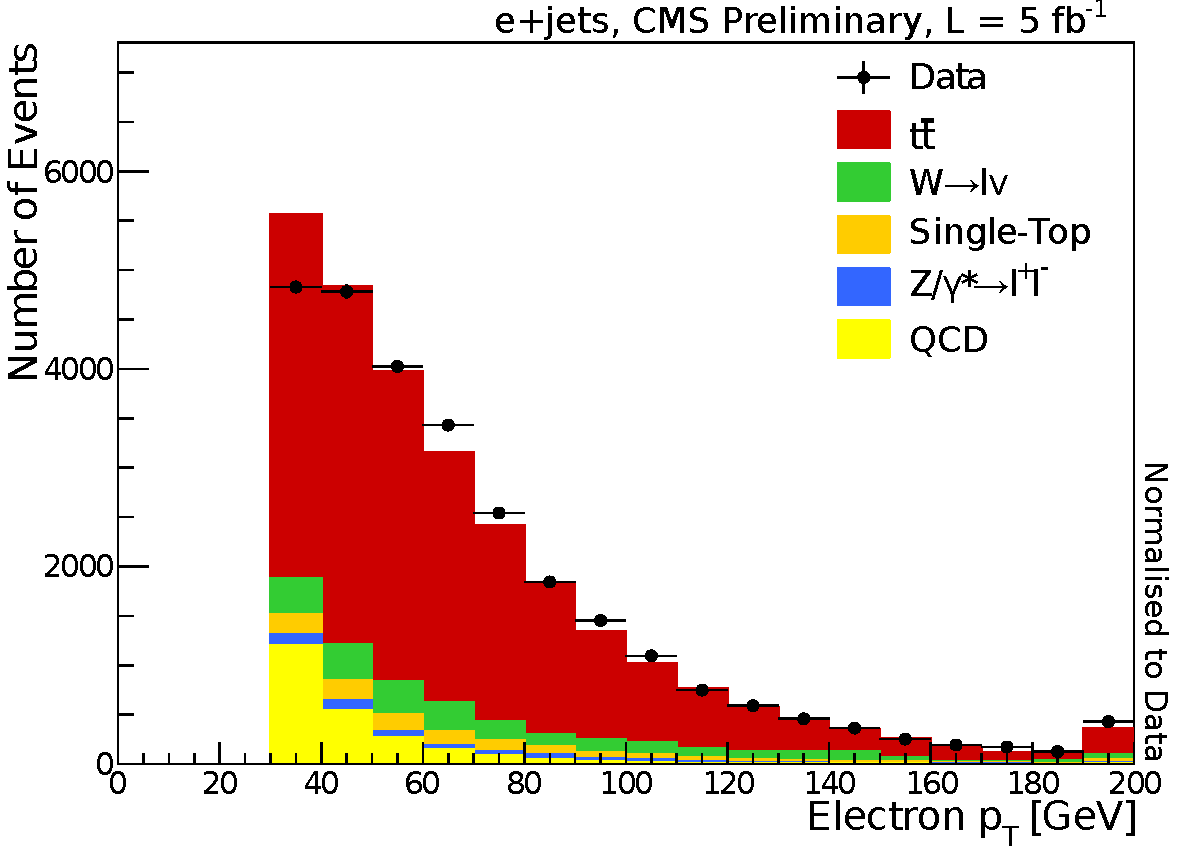
\includegraphics[width=0.5\textwidth]{cmg_electron_pt}}
   \subfloat[]{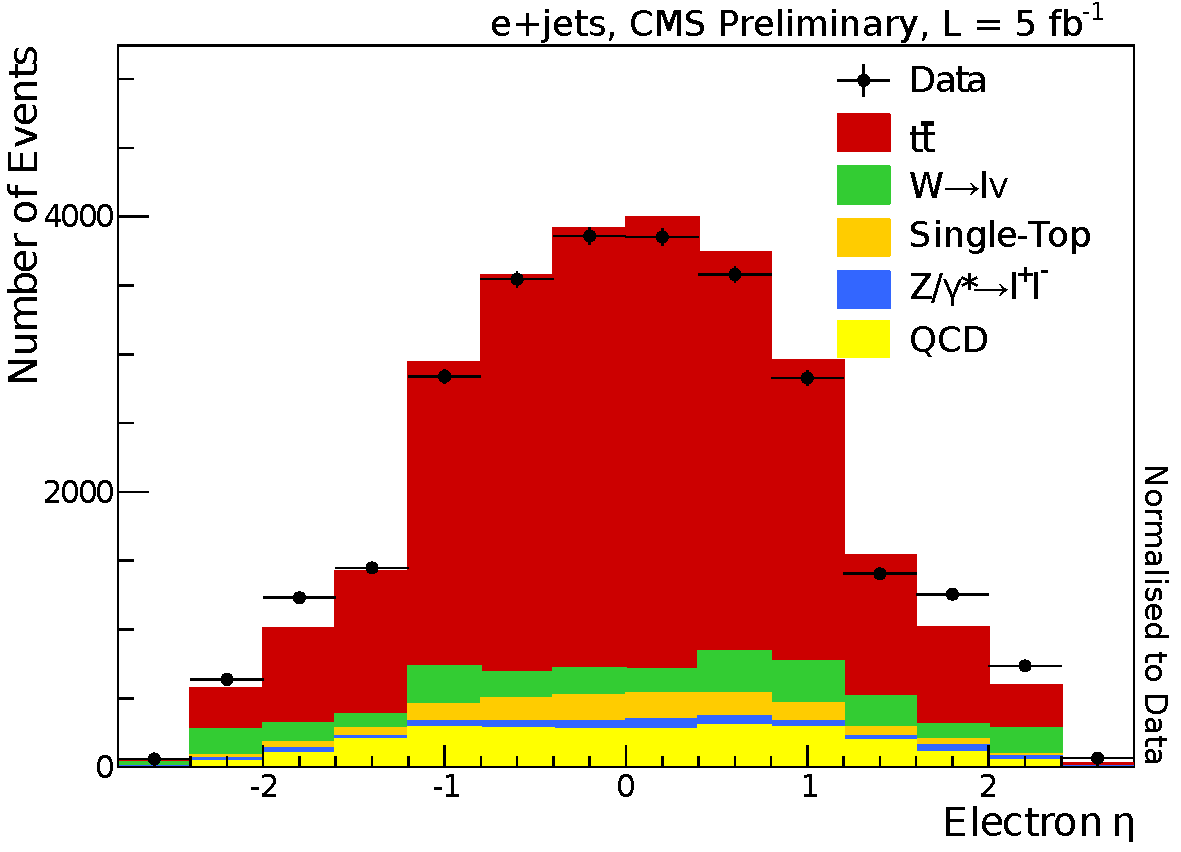
\includegraphics[width=0.5\textwidth]{cmg_electron_eta}}
   \hfill
   \subfloat[]{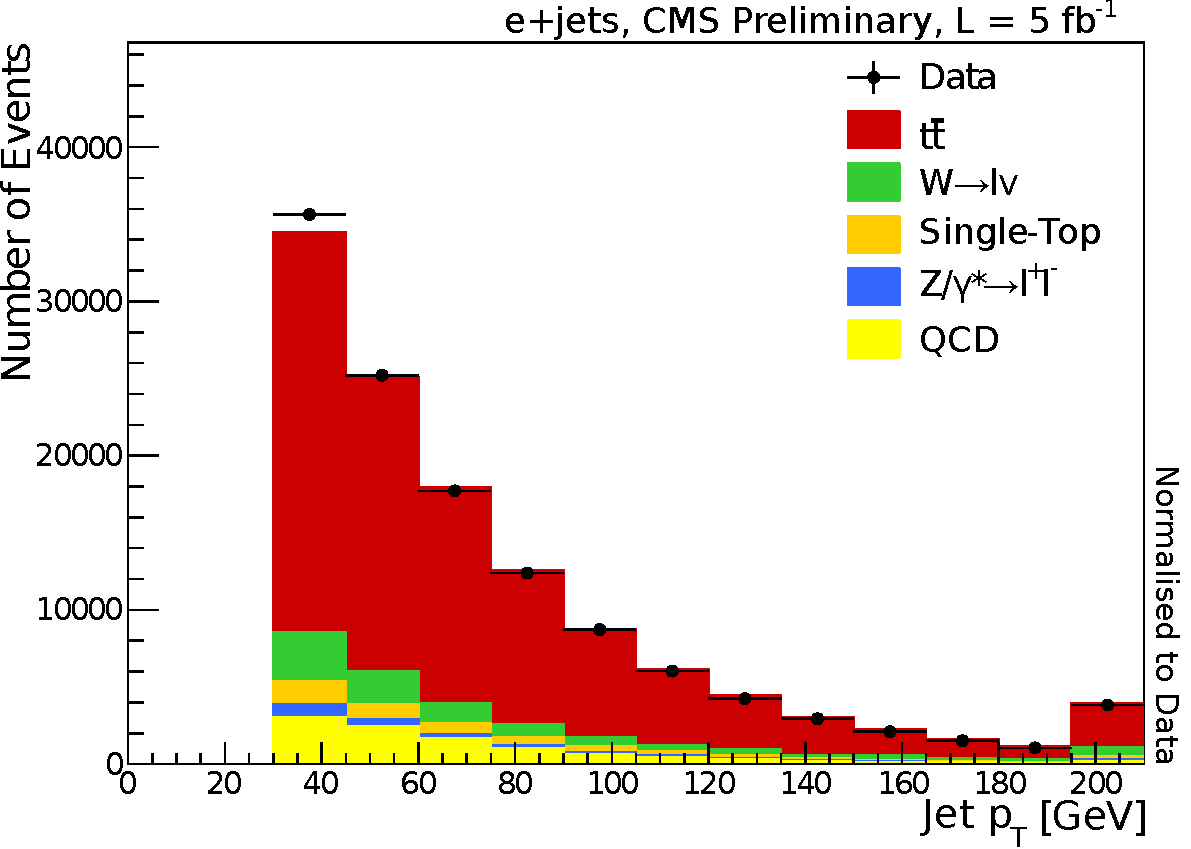
\includegraphics[width=0.5\textwidth]{cmg_jet_pt}}
   \subfloat[]{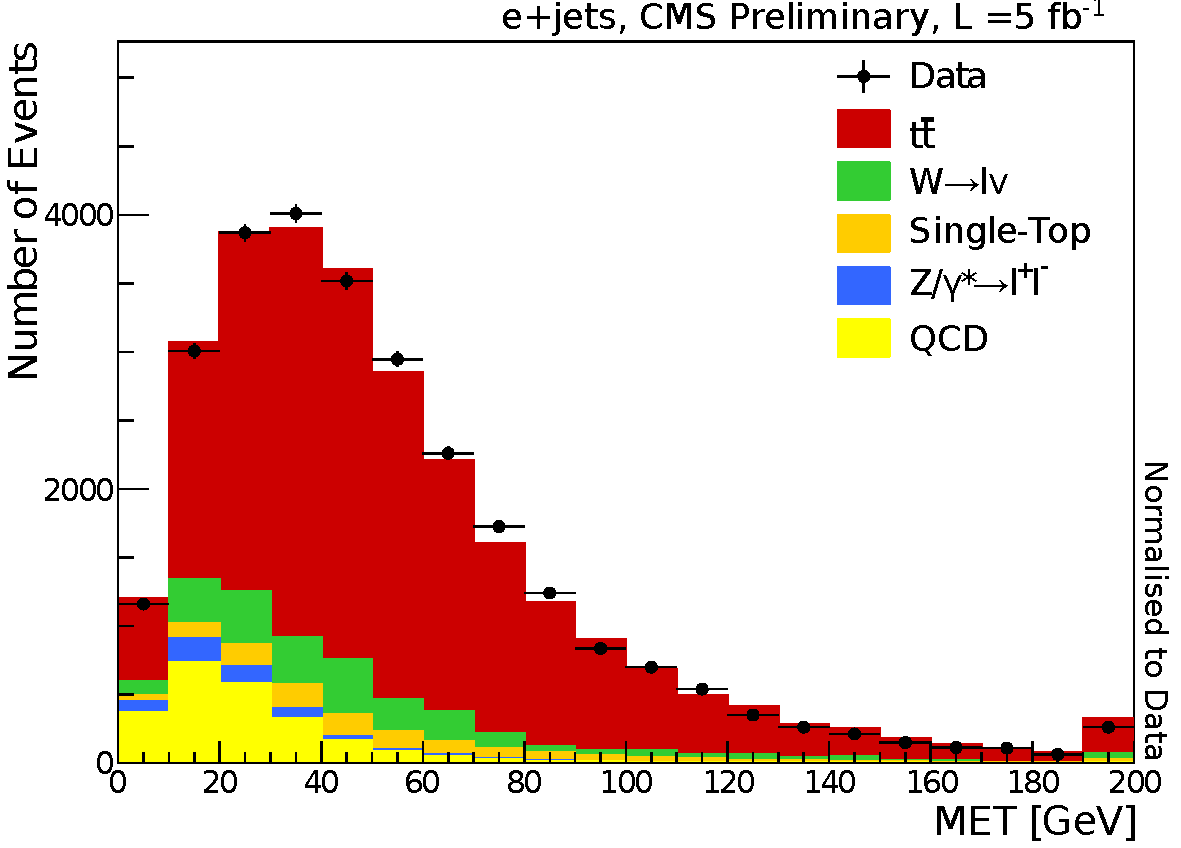
\includegraphics[width=0.5\textwidth]{cmg_met}}
   \caption{\label{fig:controlplots}Kinematic variable distributions after all selection cuts. (a) electron \pt, (b)
   electron $\eta$, (c) jet \pt for all jets passing the selection, (d) \MET.}
\end{figure}

\section{Kinematic Fit}
\label{s_top_mass:kinematic_fit}
In order to precisely measure the top quark mass, objects in the final state need to be associated with originating
partons of the top quark pair decay. In this analysis, a kinematic fit is employed to fully reconstruct the event
kinematics under the \ttbar hypothesis, thus improving the resolution of measured quantities by exploiting the knowledge
of decay process.

The \HitFit fitting package \autocite{HitFit} used in this work originates from \Dzero collaboration. Based on the SQUAW
algorithm \autocite{SQUAW} developed in Lawrence Berkeley National Laboratory, the original \HitFit code was written by
Scott Stuart Snyder in Fortran for Run I of the Tevatron. It was successfully used in the first direct measurement of
the top quark mass by \Dzero for lepton plus jets \ttbar events \autocite{D0_top_mass_1998}. The package was then
migrated to \Cplusplus for Run II of the Tevatron, and exploited in a series of \ttbar analyses including the updated
top quark mass measurement using the ideogram method \autocite{D0_top_mass_ljets_ideogram}, first measurement of the
forward-backward charge asymmetry in \ttbar production \autocite{D0_charge_assymetry} and some others.

One of the key features of the \HitFit package is its independence of specific experiments and detector geometries. The
only external dependence is on \textsc{CLHEP} \autocite{CLHEP}, a \Cplusplus library that provides utility classes for
linear algebra, geometry, vector arithmetic, etc., which was specifically developed for high energy physics simulation
and analysis software and is notably used by \GEANTfour package. In 2011 \HitFit was ported to CMSSW and later on
successfully used in a number of CMS top quark analyses, including the top mass measurement in lepton plus jets channel
\autocite{top_mass_ljets_CMS}.

\HitFit is designed to fit lepton plus jets events under the \ttbar hypothesis. Specifically, it strives to constrain
the event to a hypothesis of production of two heavy particles, each decaying into a \W boson and \cPqb quark. According
to the semi-leptonic signature, one of the \W boson decays into an electron-neutrino pair, while the other decays into a
light quark-antiquark pair.

The input to the fit includes the four-momenta of the lepton, four leading jets and missing transverse energy, as well
as their respective resolutions that were calculated using Monte Carlo samples. Since only four leading jets are used,
there are $4!=24$ ways to associate these four reconstructed jets with the partons from the \ttbar decay. The number of
permutations is reduced to $4!/2=12$ since the light jets from the hadronic \W decay are interchangeable. However, for
each hypothesis the $z$ component of neutrino four-momentum needs to be determined. This is done by requiring the two
heavy particles to have equal mass ($m_{\cPqt} = m_{\cPaqt}$), which yields to a quadratic equation which has either two
real or two complex solutions that share the real part. If case of the two real solutions the fit is performed for each
of them. If there are two complex solutions, the fit is performed once for the common real part of them, but the fit
result is included in the event content twice. Therefore, each hypothesis has two possible values of the neutrino
four-momentum, which doubles the number of permutations back to $4!=24$.

The kinematic fit is performed by minimising the $\chi^{2}$ function defined as
\begin{equation}
\chi^{2}  = (\mathbf{x} - \mathbf{x}^{m})^{T}\mathbf{G}(\mathbf{x} - \mathbf{x}^{m})
\end{equation}
where $\mathbf{x}^{m}$ is the vector or measured observables, $\mathbf{x}$ is the vector of fitted variables and
$\mathbf{G}$ is the inverse of the error matrix given by the resolutions of the observables.

The following kinematic constraints are imposed:
\begin{enumerate}[topsep=\parskip, parsep=\parskip, itemsep=\parskip, leftmargin=\leftmargin]
	\item Reconstructed top quarks from both hadronic and leptonic legs are required to have equal masses:
	\begin{equation}
		%m(t \to \ell \nu b) = m(\bar{t} \to q\bar{q} \bar{b}),
		m(\cPqt \to \ell \nu \cPqb) = m(\cPaqt \to \cPq\cPaq \cPaqb),
	\end{equation}
	\item The \W boson masses reconstructed in both hadronic and leptonic legs are fixed:
	\begin{equation}
		%m(\ell \nu) = m(q \bar{q}) = m_{W} = \SI{80.4}{\GeV}.
		m(\ell \nu) = m(\cPq\cPaq) = m_{\W} = \SI{80.4}{\GeV}.
	\end{equation}
\end{enumerate}

Apart from exploiting the knowledge of the \W mass, the \cPqb quark mass of \SI{4.7}{\GeV} is also used. Light quarks
and leptons are considered to be massless.

The full description of the fitting algorithm can be found in the appendix of the \HitFit author's PhD thesis
\autocite{Snyder}. Essentially, since the constraints are non-linear, an iterative technique is used. Starting with the
measured observables, the constraint equations are linearised by expansion in a power series around the starting point.
The minimisation is then solved with these linearised constraints, providing the new starting value for the next
minimisation step which is repeated until the $\chi^2$ converges or a maximum number of iterations is reached. Events
are rejected if there is no permutation resulting in a converging fit. Some kinematic variables for permutations giving
the best (smallest) $\chi^2$ values are shown in Figure~\ref{fig:fitplots}.

\begin{figure}[!htp]
   \centering
   \subfloat[]{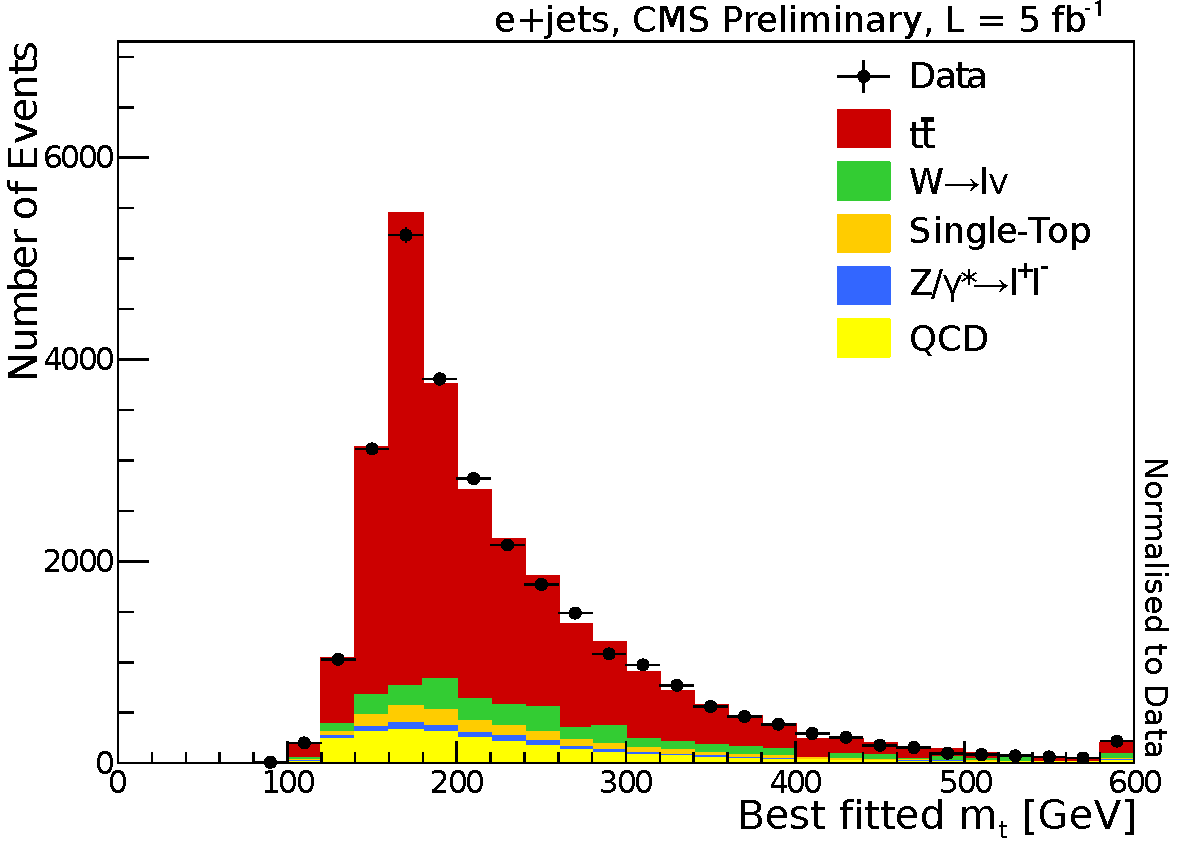
\includegraphics[width=0.5\textwidth]{hitfit_best_fitted_top_mass}}
   \subfloat[]{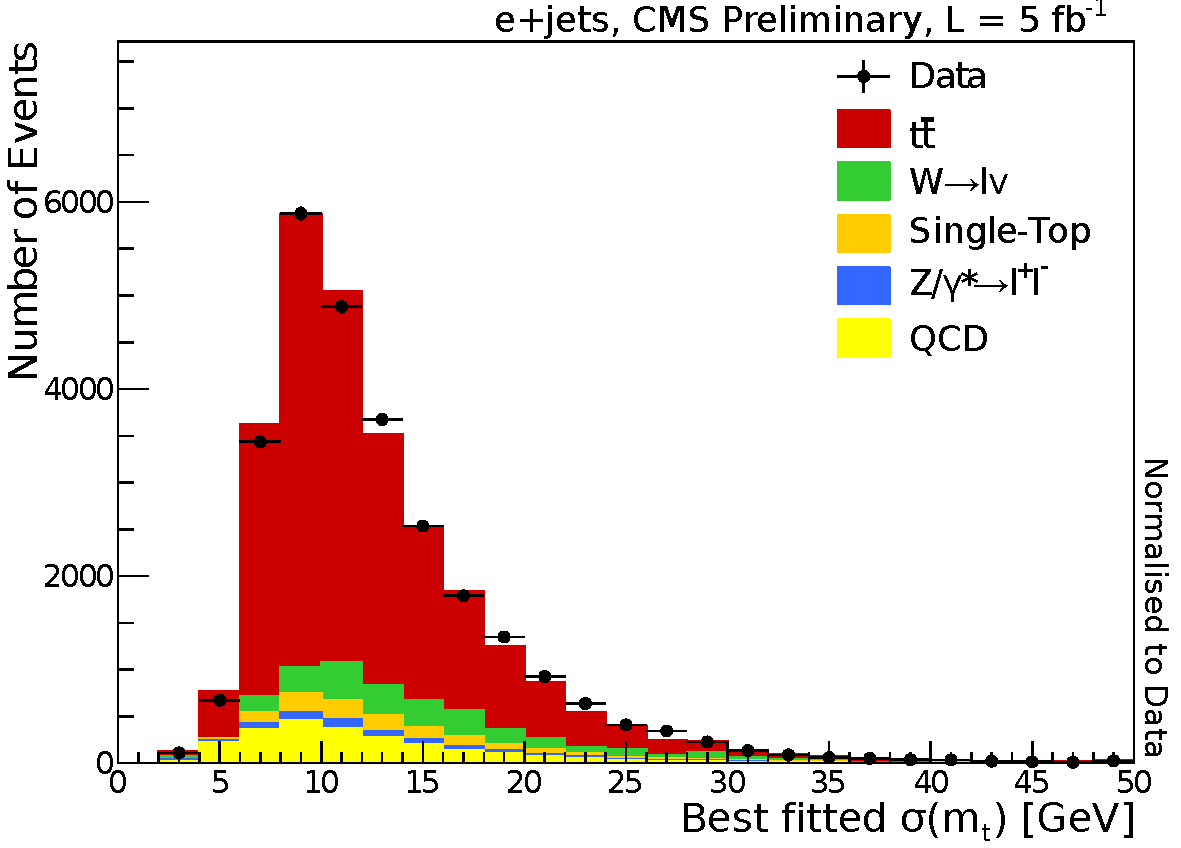
\includegraphics[width=0.5\textwidth]{hitfit_best_fitted_sigma_top_mass}}
   \hfill
   \subfloat[]{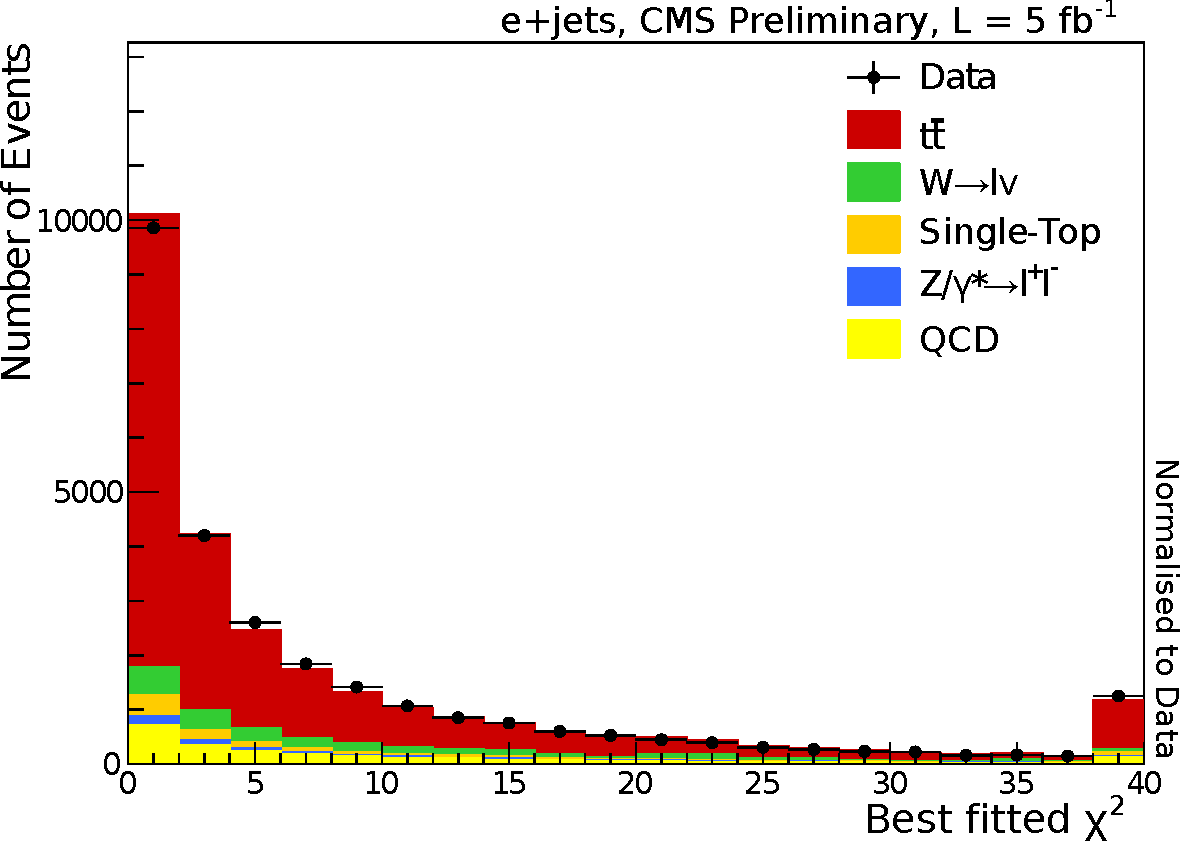
\includegraphics[width=0.5\textwidth]{hitfit_best_fitted_chi2}}
   \subfloat[]{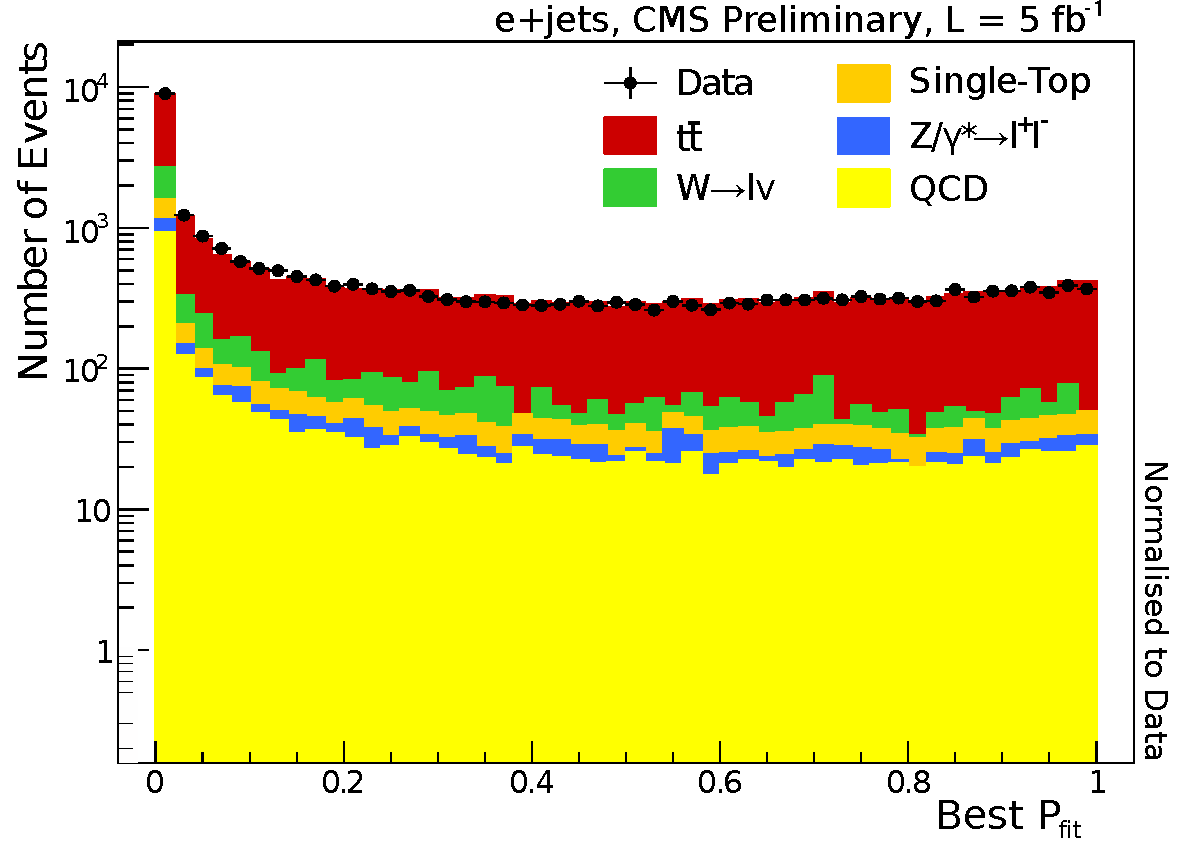
\includegraphics[width=0.5\textwidth]{hitfit_best_pfit}}
   \caption{\label{fig:fitplots}Distribution of (a) fitted top quark mass, (b) its standard deviation, (c) $\chi^{2}$
   and (d) fit probability for the best fitted hypotheses.}
\end{figure}

Typically, an event has a few permutations resulting in a converged fit. The simplest approach of picking a permutation
with the best $\chi^2$ value is disfavoured, since the Monte Carlo studies have shown that the correct permutation
does not necessarily have the best $\chi^2$. This value can change drastically with relatively small variations of the
input parameters, as different permutations may obtain the smallest value of $\chi^2$. On the other hand, some solutions
yield very large $\chi^2$ value, which typically happens for badly reconstructed or background events. Therefore, a
loose cut of $\chi^2=20$ is applied for all permutations on the output of the converged fit. This is the final
selection criteria on top of the reference selection mentioned in Section~\ref{s_top_mass:event_selection}.

%Table \ref{tab:chi2_eff} list the number of events which pass the reference selection only, and number of events which
% pass both the reference selection and the loose $\chi^{2}$ cut.

The compatibility of a permutation with the \ttbar hypothesis is quantified by the following fit probability:
\begin{equation}
	P_{\textrm{fit}} = \textrm{exp}(-\frac{1}{2}\chi^2).
\end{equation}

This probability is used in the next step of the analysis, referred to as the Ideogram Method.


\section{Ideogram Method}
\label{s_top_mass:ideogram_method}
The ideogram method is a powerful mass extraction technique. Its main idea lies in finding the likelihood distribution
of the particle mass given the particular data sample, which is performed by evaluating the likelihood of measured
observables given a generated particle mass for each event in the sample. The signal likelihood is evaluated from the
theoretically expected Breit-Wigner distribution convoluted with the Gaussian experimental resolution on event-by-event
basis. The whole procedure is calibrated using Monte Carlo simulation of a series of particle masses in the expected
region.

%All selected jet-parton permutations from the output of the kinematic fit are weighted by their fit probability
%$P_{\textrm{fit}}$.

One of the first applications of the ideogram method tracks back to the \W boson mass measurement by the \textsc{DELPHI}
Collaboration at CERN LEP collider \autocite{DELPHI_1998, DELPHI_2008}. It was later used for a series of top quark mass
measurements, including the \Dzero measurement in lepton plus jets channel \autocite{D0_top_mass_ljets_ideogram} and CDF
measurement in all-hadronic channel \autocite{CDF_ideogram}.
\subsection{Event likelihood}
\label{ss_top_mass:event_likelihood}
The basis of the ideogram method is the event likelihood, also referred to as the ideogram. For each event in the
sample, a likelihood to observe the event is calculated as a function of the assumed top quark mass, $m_{t}$. There are
two terms in the likelihood. One term corresponds to the probability for the event to be a $t\bar{t}$ signal, another
term corresponds to the probability for the event to be a background event.

\begin{equation}
\mathcal{L}_{event}\left(x|m_{t},f_{t\bar{t}}\right) = f_{t\bar{t}} P_{t\bar{t}}\left(x|m_{t}\right) + \left(1 -
f_{t\bar{t}}\right)P_{bkg}\left(x\right).
\label{eq:EventLikelihood}
\end{equation}

In this equation, $x$ is the set of variables which characterizes the event, $f_{t\bar{t}}$ is the fraction of
$t\bar{t}$ event in the data sample, and $P_{t\bar{t}}$ and $P_{bkg}$ are the probability densities for $t\bar{t}$ and
background event, respectively.  The event observables $x$ are the mass information from the kinematic fit for each
possible jet to quark assignments and neutrino solutions: the fitted mass $m_{i}$, the estimated uncertainties for each
fitted mass $\sigma_{i}$, and the goodness-of-fit $\chi^{2}_{i}$.

The $t\bar{t}$ probability density depends on both $x$ and $m_{t}$. The background probability density only depends on
$x$ and doesn't depend on $m_{t}$.  We assume that the background probability can be described by the probability
density for $W+$jets events only. The contributions from $W+$ heavy flavour jets, single top, $Z+$jets, and QCD events
are expected to be small.  Furthermore, their probability densities have similar shape to that of $W+$jets events. Note
that in the final MC calibration we include all above backgrounds to evaluate and correct for a possible bias due to
this (and other) approximation(s).

The probabilities are calculated as a weighted sum over all possible combinations of jet to quark assignments and
neutrino solutions.  The relative probability for each solution to fulfil the $t\bar{t}$ lepton+jets event hypothesis
is proportional to $\exp\left(-\frac{1}{2}\chi^{2}\right)$.  However, some solutions yield very large $\chi^{2}$ value
from the kinematic fit. Those are mostly either badly misreconstructed events or background events which don't carry top
quark mass information.  Therefore, we take only solutions which have $\chi^{2}$ value from the kinematic fit smaller
than 20.

\subsection{Inclusion of b-tagging information in the likelihood}

This analysis uses b-tagging information to further separate
\ttbar signal and background, and to separate \ttbar signal with correct and wrong jet permutation assignments.  We use
the Combined Secondary Vertex (CSV) tagging algorithm at the Medium working point (requiring CSV discriminant to be
greater than 0.679).
%This %is the same algorithm and working point used by the reference \ttbar %cross-section with b-tagging analysis
%\cite{CMS-PAS-TOP-11-003???}.

If one or more jets in the event is b-tagged, we assign an additional relative weight, $w_{\rm btag}$, representing the
likelihood that the observed b-tags are compatible with the jet flavour assignment hypothesis for that particular jet
permutation.

\begin{equation}
w_{\rm btag} = \prod_{j} p^{j}
\end{equation}

where the index $j$ runs over all the jets considered in the fit.  The b tag probability $p^{j}$ can be either
$\varepsilon_{l}$, $(1 - \varepsilon_{l})$, $\varepsilon_{b}$, or $(1 - \varepsilon_{b})$, depending on the hypothesized
flavour of the jet (light jet or b jet), and whether the jet is b-tagged or not.  For the light jet mistag rate, we
assume that the $W boson$ can decay into $c\bar{s}$ and $u\bar{d}$ pair, and thus take into account the higher tagging
rate for c quark jet.

\subsection{Correct and wrong permutation $t\bar{t}$ signal probability}

The $t\bar{t}$ signal probability contains two terms and can be expressed as:
\begin{equation}
P_{t\bar{t}}\left(x|m_{t}\right) = \sum_{i}^{24} w_{i} \left( f_{cp}
\cdot \int^{m_{max}}_{m_{min}} dm'
G\left(m'|m_{i},\sigma_{i}\right) RBW
\left(m' |m_{t},\Gamma_{t}\right)
+ (1 - f_{cp})WP(m_{i}|m_{t})\right)
\end{equation}
The first term expresses the probability that a solution has the correct jets to quarks assignment
(correct-permutation). The second term expresses the probability that a solution doesn't have the correct jets to quarks
assignment (wrong-permutation).

The correct-permutation probability is given as a convolution of a Gaussian resolution function $G(m'|m_{i},\sigma_{i})$
and relativistic Breit-Wigner distribution $RBW(m'|m_{t},\Gamma_{t})$. The Gaussian is centred at the value of fitted
mass $m_{i}$ and has a width of the estimated fitted mass uncertainty $\sigma_{i}$.  It describes the estimated mass
resolution for each jet/neutrino solutions. The relativistic Breit-Wigner (RBW) describes the distribution of the
invariant mass $m'$ of top quark (or antitop quark) in $t\bar{t}$ event for a given assumed top quark mass $m_{t}$ and
top quark width $\Gamma_{t}$.  We set the value of top quark width to 2 GeV.

We use the following form of the RBW,
\begin{equation}
RBW(m|m_{0},\Gamma_{0}) \propto \frac{m^{2}}{\left(m^{2} - m_{0}^{2}
\right)^{2} + m^{4}\frac{\Gamma_{0}^{2}}{m_{0}^{2}}}
\end{equation}
as suggested by $s-$dependence of the phase space and Standard Model electroweak corrections, see equations (1.35) and
(1.40) in \cite{:2005ema}.

% \begin{figure}[!htpb]
% \begin{center}
%     \subfigure[]{\includegraphics[width=0.49\textwidth]{figs/EJetsTtLJets1665FourJetInclCpGaussFit}}
%     \subfigure[]{\includegraphics[width=0.49\textwidth]{figs/MuJetsTtLJets1665FourJetInclCpGaussFit}}
% 	\caption{\label{fig:WJetsDensity2}
% 	Plots of the fitted mass for the $t\bar{t}$ events with
%     correct-permutation.  Left is for the $e+$jets channel,
% 	right is for the $\mu$+jets channel.}
% \end{center}
% \end{figure}

The wrong-permutation probability density is derived by fitting analytical functions to the fitted mass distribution of
jet/neutrino solutions which have wrong jets to quarks assignment in Monte Carlo $t\bar{t}$ event sample.  There are two
kinds of events with wrong jets to quarks assignment.  The first kind of events have the four leading jets matched to
quarks from $t\bar{t}$ decay, but the jets are not assigned to quarks correctly.  The second kind of events have one or
more of the four leading jets coming from radiated gluon instead of quarks from $t\bar{t}$ decay.  We found that both
type of events have similar shape and decided to group them together as events which have the wrong-permutation jets to
quarks assignment.

For each event which has at least one converging jet/neutrino solutions, we removed the jet/neutrino solutions which
have the correct jets to quarks assignment. We then plotted the fitted mass from the remaining jet/neutrino solutions.
Each entry is weighed by the same weight used in the event likelihood.

We found that the fitted mass distribution for the wrong-permutation \ttbar can be described very well by the Crystal
Ball functions with exponential order 5, with their parameters $\mu$, $\sigma$, and $\alpha$ can be parametrized as
functions of top quark mass.  Figure \ref{fig:TtWpDensity} shows the fitted mass spectra for the wrong-permutation
combinations of \ttbar events, with three different masses: 166.5, 172.5, and 178.5 GeV.

% \begin{figure}[!htpb]
% \begin{center}
%     \subfigure[]{\includegraphics[width=0.41\textwidth]{figs/CbFitTagWpm4jiEJetsTtLJets1665}}
%     \subfigure[]{\includegraphics[width=0.41\textwidth]{figs/CbFitTagWpm4jiMuJetsTtLJets1665}}

%     \subfigure[]{\includegraphics[width=0.41\textwidth]{figs/CbFitTagWpm4jiEJetsTtLJets1725}}
%     \subfigure[]{\includegraphics[width=0.41\textwidth]{figs/CbFitTagWpm4jiMuJetsTtLJets1725}}

%     \subfigure[]{\includegraphics[width=0.41\textwidth]{figs/CbFitTagWpm4jiEJetsTtLJets1785}}
%     \subfigure[]{\includegraphics[width=0.41\textwidth]{figs/CbFitTagWpm4jiMuJetsTtLJets1785}}
% 	\caption{\label{fig:TtWpDensity}
% 	Plots of the fitted mass for the $t\bar{t}$ events with
%     wrong-permutation. Left is
% 	for the $e+$jets channel, right is for the $\mu$+jets channel.  Top
%     row is for $m_{t} = 166.5$ GeV, middle row is for $m_{t} = 172.5$
%     GeV, bottom row is for $m_{t} = 178.5$ GeV.}
% \end{center}
% \end{figure}

\subsection{Background probability}

The shapes of the background probability are taken from the fitted mass spectrum in $W+$jets Monte Carlo samples. We
perform the kinematic fit to $W+$jets Monte Carlo events and plot all fitted mass for all jet permutations, weighted by
the $\chi^{2}$ and b-tagging weights as described before.  We found that the fitted mass spectra of $W+$jets events can
be described by a Landau distribution, with different parametrization for $e$+jets and $\mu$+jets channel.  Figure
\ref{fig:WJetsDensity} shows the fitted mass spectra for the $W+$jets events.

% \begin{figure}[!htpb]
% \begin{center}
%     \subfigure[]{\includegraphics[width=0.49\textwidth]{figs/EJetsWJetsFourJetInclMass}}
%     \subfigure[]{\includegraphics[width=0.49\textwidth]{figs/MuJetsWJetsFourJetInclMass}}
% 	\caption{\label{fig:WJetsDensity}
% 	Plots of the fitted mass in $W+$jets sample.  Left is
% 	for the $e+$jets channel, right is for the $\mu$+jets channel.}
% \end{center}
% \end{figure}


\subsection{Combined likelihood fit}
\label{ss_top_mass:likelihood_fit}

The likelihood for the entire lepton+jets sample is calculated as the product of each event likelihood curve,
\begin{equation}
\mathcal{L}_{sample} = \prod_{\rm all~event}
\mathcal{L}_{event}\left(x|m_{t},f_{t\bar{t}}\right).
\label{eq:CombinedLikelihood}
\end{equation}
Difference in sample composition between subsamples ($e$+jets and $\mu$+jets, 0-tag and 1-tag and 2-tag) are taken into
account in the likelihood.

In practice, what is done is summing over the negative likelihood for all events in the sample.  For each event, the
likelihood is evaluated as a function of top quark mass.  The minima of the sum of log likelihood curve is then taken as
the most probable value of top quark mass.

\section{Mass calibration}
\label{s_top_mass:calibration}

\section{Systematic Uncertainties}
\label{s_top_mass:systematics}

\section{Results}
\label{s_top_mass:results}

\section{Summary}
\label{s_top_mass:summary}


% ------------------------------------------------------------------------


%%% Local Variables: 
%%% mode: latex
%%% TeX-master: "../thesis"
%%% End: 

%!TEX root = ../thesis.tex

\chapter[Top Quark Pair Differential Cross Section Measurement]{Top Quark Pair Differential \\Cross Section Measurement}
\label{c:xsection_analysis}
\ifpdf
    \graphicspath{{06_Cross_section_analysis/plots/}}
\else
    \graphicspath{{06_Cross_section_analysis/plots/EPS/}{06_Cross_section_analysis/plots/}}
\fi

% ------------------------------------------------------------------------
Measurement of the differential cross section of the top quark pairs with respect to different variables is an important
precision measurement, and provides a sensitive probe for new physics. For instance, deviations in the tail of the
missing transverse energy distribution could signal new resonances with invisible particles produced in association with
top quarks.

The analysis described in this chapter represents the top quark differential cross section measurement with respect to
event-level (or global) distributions, including the missing transverse momentum (\MET), the scalar sum of jet
transverse momenta (\HT), the scalar sum of the transverse momenta of all objects in the event (\ST), and both the
transverse mass (\MT) and transverse momentum (\WPT) of the leptonically decaying \W boson produced in the top quark
decay \autocite{xsection_PAS_7TeV, xsection_PAS_8TeV}. The analysis is focused on semileptonic \ttbar decays, where a
lepton is either an electron or a muon. The cross section measurement is performed to validate different Monte Carlo
generators and theoretical predictions of the effects due to variations of various modelling parameters.

\section{Data and Simulation}
\label{s_xsection:data_and_simulation}

\subsection{Data}
\label{ss_xsection:data}
This analysis uses the full 2012 dataset collected by the CMS detector at a centre of mass energy of \SI{8}{\TeV}, with
a total integrated luminosity of \SI{19.7}{\fbinv}. Only certified events were used in the data, i.e.\ from such
preriods of data-taking when all of the detector subsystems were functioning with no errors. Depending on the channel,
the data were preselected with the single electron or single muon trigger. The preselection procedure as well as full
event selection will be described in Section~\ref{s_xsection:event_selection}.

\subsection{Monte Carlo samples}
\label{ss_xsection:MC_samples}
The Monte Carlo generators used in this work were presented in Section~\ref{ss:MC_generators}. The list of signal and
background MC samples is shown in Table~\ref{tab:xsection_mc_samples}, and is broadly similar to that from the top quark
mass analysis. In addition, the signal \ttjets sample is also available with \POWHEG and \MCATNLO generators in order to
be able to differentiate between them. Moreover, to extend the statistics of the \W/\ZpJets samples, they were generated
in four exclusive jet multiplicity bins: \W/\Z boson plus one/two/three and at least four jets.

Table~\ref{tab:xsection_electron_qcd_samples} presents the list of QCD multi-jet background and $\gamma$ + jets samples
used in the estimation of the QCD background in the electron plus jets channel. The analogous set of muon-enriched QCD
samples used in the muon plus jets channel is shown in Table~\ref{tab:xsection_muon_qcd_samples}. Although the QCD
background is estimated using data-driven techniques in both channels (see Section~\ref{s_xsection:data_driven_QCD}),
the MC simulation is still used for normalisation purposes.
% Mention the systematic samples (Table~\ref{tab:xsection_systematic_samples})

\begin{table}[!htbp]
\centering
\caption{Signal and background Monte Carlo samples with cross sections at $\sqrt s =
\SI{8}{\TeV}$, numbers of generated events and corresponding integrated
luminosities.}
\label{tab:xsection_mc_samples}
\begin{tabular}{|l|l|r|r|r|}
\toprule
Process & Generator & $\sigma$ (\pb) & \# events & $\int\lumi dt$ (\fbinv)\\
\midrule
\ttjets, \mtop = \SI{172.5}{\GeV} & \MADGRAPH & 245.8 & 6854416 & 27.9\\
\ttjets, \mtop = \SI{172.5}{\GeV} & \POWHEG  & 245.8 & 21675970 & 88.2\\
\ttjets, \mtop = \SI{172.5}{\GeV} & \MCATNLO & 245.8 & 32706581 & 133.1\\
\midrule
\WpJets ($\W \rightarrow l\nu$) & \MADGRAPH & & & \\
\hspace{5 mm}\W + 1 jet & & 5400.0 & 23141598 & 4.3 \\
\hspace{5 mm}\W + 2 jet & & 1750.0 & 34044921 & 19.5 \\
\hspace{5 mm}\W + 3 jet & & 519.0 & 15539503 & 29.9 \\
\hspace{5 mm}\W + 4 jet & & 214.0 & 13349346 & 62.4 \\
\midrule
$\Z/\gamma^* \rightarrow l^+l^- $ + jets, $m(ll) > \SI{50}{\GeV}$ & \MADGRAPH & & & \\
\hspace{5 mm}\Z + 1 jet & & 561.0 & 24045248 & 42.9 \\
\hspace{5 mm}\Z + 2 jet & & 181.0 & 21852156 & 120.7 \\
\hspace{5 mm}\Z + 3 jet & & 51.1 & 11015445 & 215.6 \\
\hspace{5 mm}\Z + 4 jet & & 23.04 & 6402827 & 277.9 \\
\midrule
Single top & \POWHEG & & & \\
\hspace{5 mm} top t-channel & & 55.5 & 3758227 & 67.7 \\
\hspace{5 mm} anti-top t-channel & & 30.0 & 1935072 & 64.5 \\
\hspace{5 mm} top s-channel & & 3.89 & 259961 & 66.8 \\
\hspace{5 mm} anti-top s-channel & & 1.76 & 139974 & 79.5 \\
\hspace{5 mm} top tW-channel & & 11.18 & 497658 & 44.5 \\
\hspace{5 mm} anti-top tW-channel & & 11.18 & 493460 & 44.1 \\
\bottomrule
\end{tabular}
\end{table}

\begin{table}[!htbp] 
\centering
\caption{QCD multi-jet background and $\gamma$ + jets MC samples used in the electron plus jets channel
with cross sections at $\sqrt s = \SI{8}{\TeV}$, numbers of generated events and corresponding integrated luminosities.
% EM-enriched samples are preselected to include jets with higher electromagnetic content;
% $\cPqb/\cPqc \rightarrow e\nu$ samples are preselected to include leptonic ($e\nu$) in-flight decays of b- and c-quarks.
}
\label{tab:xsection_electron_qcd_samples}
\resizebox{\textwidth}{!}{
\begin{tabular}{|l|l|r|r|r|r|}
\toprule
Process & Generator & $\sigma$ (\pb) & filter efficiency & \# events & $\int\lumi dt$ (\fbinv)\\
\midrule
QCD ($e/\gamma$ enriched)  & \PYTHIA & & & & \\
\hspace{5 mm}\SIrange[range-phrase = $~<\pthat<~$]{20}{30}{\GeV} 	& & \num{2.886d8} 	& \num{1.01d-2} & 34339883 & \num{1.2d-2} \\
\hspace{5 mm}\SIrange[range-phrase = $~<\pthat<~$]{30}{80}{\GeV} 	& & \num{7.433d7} 	& \num{6.21d-2} & 32537408 & \num{7.0d-3} \\
\hspace{5 mm}\SIrange[range-phrase = $~<\pthat<~$]{80}{170}{\GeV} 	& & \num{1.191d6}  	& \num{0.154} &  34542763 & \num{0.19} \\
\hspace{5 mm}\SIrange[range-phrase = $~<\pthat<~$]{170}{250}{\GeV} 	& & \num{30990.0} 	& \num{0.148} & 22862259 & \num{5.0} \\
\hspace{5 mm}\SIrange[range-phrase = $~<\pthat<~$]{250}{350}{\GeV} 	& & \num{4250.0} 	& \num{0.131} &  32505856 & \num{58.4} \\
\hspace{5 mm}$\pthat >$ \SI{350}{\GeV}  							& &	\num{810.0}  	& \num{0.11} &  33981105 & \num{381.4} \\
\midrule
QCD ($\cPqb/\cPqc \rightarrow e\nu$) & \PYTHIA & & & & \\
\hspace{5 mm}\SIrange[range-phrase = $~<\pthat<~$]{20}{30}{\GeV} 	& & \num{2.886d8} 	& \num{5.8d-4} & 1740229 & \num{1.0d-2} \\
\hspace{5 mm}\SIrange[range-phrase = $~<\pthat<~$]{30}{80}{\GeV} 	& & \num{7.433d7} 	& \num{2.25d-3} & 2048152 & \num{1.2d-2} \\
\hspace{5 mm}\SIrange[range-phrase = $~<\pthat<~$]{80}{170}{\GeV} 	& & \num{1.191d6}  	& \num{1.09d-2} & 1945525 & \num{0.15} \\
\hspace{5 mm}\SIrange[range-phrase = $~<\pthat<~$]{170}{250}{\GeV} 	& & \num{30990.0} 	& \num{2.04d-2} & 1948112 & \num{3.1} \\
\hspace{5 mm}\SIrange[range-phrase = $~<\pthat<~$]{250}{350}{\GeV} 	& & \num{4250.0}  	& \num{2.43d-2} & 2026521 & \num{19.6} \\
\hspace{5 mm}$\pthat >$ \SI{350}{\GeV} 								& &	\num{810.0}  	& \num{2.95d-2} & 1948532 & \num{81.5} \\
\midrule
$\gamma$ + jets & \MADGRAPH & & & & \\
\hspace{5 mm}\SIrange[range-phrase = $~<\HT<~$]{200}{400}{\GeV} & & \num{960.5} & 1 & 10479625 & \num{10.9} \\
\hspace{5 mm}$\HT >$ \SI{400}{\GeV} & & \num{107.5} & 1 & 1611963 & \num{15.0} \\
\bottomrule
\end{tabular}
}
\end{table}

\begin{table}[!htbp] 
\centering
\caption{QCD multi-jet background MC samples used in the muon plus jets channel with cross sections at $\sqrt s =
\SI{8}{\TeV}$, numbers of generated events and corresponding integrated luminosities.}
\label{tab:xsection_muon_qcd_samples}
\resizebox{\textwidth}{!}{
\begin{tabular}{|l|l|r|r|r|r|}
\toprule
Process & Generator & $\sigma$ (\pb) & filter efficiency & \# events & $\int\lumi dt$ (\fbinv)\\
\midrule
QCD ($\mu$ enriched)  & \PYTHIA & & & & \\
\hspace{5 mm}\SIrange[range-phrase = $~<\pthat<~$]{15}{20}{\GeV} 	& & \num{7.022d8} 	& \num{3.9d-3}	& 1722681	& \num{6.3d-4} \\
\hspace{5 mm}\SIrange[range-phrase = $~<\pthat<~$]{20}{30}{\GeV} 	& & \num{2.87d8} 	& \num{6.5d-3}	& 8486904	& \num{4.5d-3} \\
\hspace{5 mm}\SIrange[range-phrase = $~<\pthat<~$]{30}{50}{\GeV} 	& & \num{6.609d7} 	& \num{1.22d-2}	& 9560265	& \num{1.2d-2} \\
\hspace{5 mm}\SIrange[range-phrase = $~<\pthat<~$]{50}{80}{\GeV} 	& & \num{8.082d6} 	& \num{2.18d-2}	& 10365230	& \num{5.9d-2} \\
\hspace{5 mm}\SIrange[range-phrase = $~<\pthat<~$]{80}{120}{\GeV} 	& & \num{1.024d6}	& \num{3.95d-2}	& 9238642	& \num{0.23} \\
\hspace{5 mm}\SIrange[range-phrase = $~<\pthat<~$]{120}{170}{\GeV} 	& & \num{1.578d5}	& \num{4.73d-2}	& 8501935	& \num{1.1} \\
\hspace{5 mm}\SIrange[range-phrase = $~<\pthat<~$]{170}{300}{\GeV} 	& & \num{34020.0}	& \num{6.76d-2}	& 7669947	& \num{3.3} \\
\hspace{5 mm}\SIrange[range-phrase = $~<\pthat<~$]{300}{470}{\GeV} 	& & \num{1757.0}	& \num{8.64d-2}	& 7832261	& \num{51.6} \\
\hspace{5 mm}\SIrange[range-phrase = $~<\pthat<~$]{470}{600}{\GeV} 	& & \num{115.2}		& \num{0.102}	& 3783069	& \num{322.0} \\
\hspace{5 mm}\SIrange[range-phrase = $~<\pthat<~$]{600}{800}{\GeV} 	& & \num{27.01}		& \num{0.0996}	& 4119000	& \num{1531.1} \\
\hspace{5 mm}\SIrange[range-phrase = $~<\pthat<~$]{800}{1000}{\GeV} & & \num{3.57}		& \num{0.1033}	& 4107853	& \num{11139.0} \\
\hspace{5 mm}$\pthat >$ \SI{1000}{\GeV}  							& &	\num{0.774}		& \num{0.1097}	& 3873970	& \num{45625.6} \\
\bottomrule
\end{tabular}
}
\end{table}

\begin{table}[!htbp]
\centering
\caption{Systematic MC samples with cross sections at $\sqrt s =
\SI{8}{\TeV}$, numbers of generated events and corresponding integrated
luminosities. Factorisation scale $Q$ and matching threshold systematic
uncertainties are estimated with variations of \ttjets, \WpJets and \ZpJets
samples.}
\label{tab:xsection_systematic_samples}
\begin{tabular}{|l|l|r|r|r|}
\toprule
Process & Generator & $\sigma$ (\pb) & \# events & $\int\lumi dt$ (\fbinv)\\
\midrule
\ttjets & \MADGRAPH & & & \\
\hspace{5 mm}$0.5~\times$ matching threshold 	& & 245.8 & 5476728	& 10.2 \\
\hspace{5 mm}$2~\times$ matching threshold  	& & 245.8 & 5306710	& 25.5 \\
\hspace{5 mm}$0.5\times Q$  					& & 245.8 & 5387181 & 25.4 \\
\hspace{5 mm}$2\times Q$ 						& & 245.8 & 5009488 & 23.4 \\
\midrule
\WpJets ($\W \rightarrow l\nu$) & \MADGRAPH & & & \\
\hspace{5 mm}$0.5~\times$ matching threshold 	& & 29690 & 21364637 & 0.7 \\
\hspace{5 mm}$2~\times$ matching threshold 		& & 30290 & 20976082 & 0.7 \\
\hspace{5 mm}$0.5 \times Q$ 					& & 33300 & 20719363 & 0.6 \\
\hspace{5 mm}$2 \times Q$ 						& & 32000 & 20784770 & 0.6 \\
\midrule
\ZpJets ($\Z \rightarrow ll$) & \MADGRAPH & & & \\
\hspace{5 mm}$0.5~\times$ matching threshold 	& & 2888 & 2112387 & 0.6 \\
\hspace{5 mm}$2~\times$ matching threshold 		& & 2915 & 1985529 & 0.7 \\
\hspace{5 mm}$0.5 \times Q$ 					& & 3312 & 1934901 & 0.6 \\
\hspace{5 mm}$2 \times Q$ 						& & 2954 & 2170270 & 0.7 \\
\bottomrule
\end{tabular}
\end{table}

% WARNING: V+Jets systematic samples cross sections are 7 TeV ones (taken from PREP)
% Does this affect the measurement of the systematics?

\newpage
\subsection{Pile-up reweighting}
\label{sss_xsection:pileup_reweighting}
Since the number of simulated pile-up interactions does not necessarily represent the same distribution in data, a
reweighting procedure for MC events is required. To produce the weights, measured instantaneous luminosity is used to
obtain a distribution of true pile-up vertices in data, i.e.\ before any vertex reconstruction inefficiencies. This
distribution is then divided by the simulated one, and for each number of pile-up interactions, the weight is
calculated. Figure~\ref{fig:pileup_vertices} shows the number of interactions before and after reweighting for both
electron and muon channels. Evidently, the reweighting procedure helps to achieve a good agreement between data and
simulation.

\begin{figure}[!htpb]
	\centering
	\subfloat[]{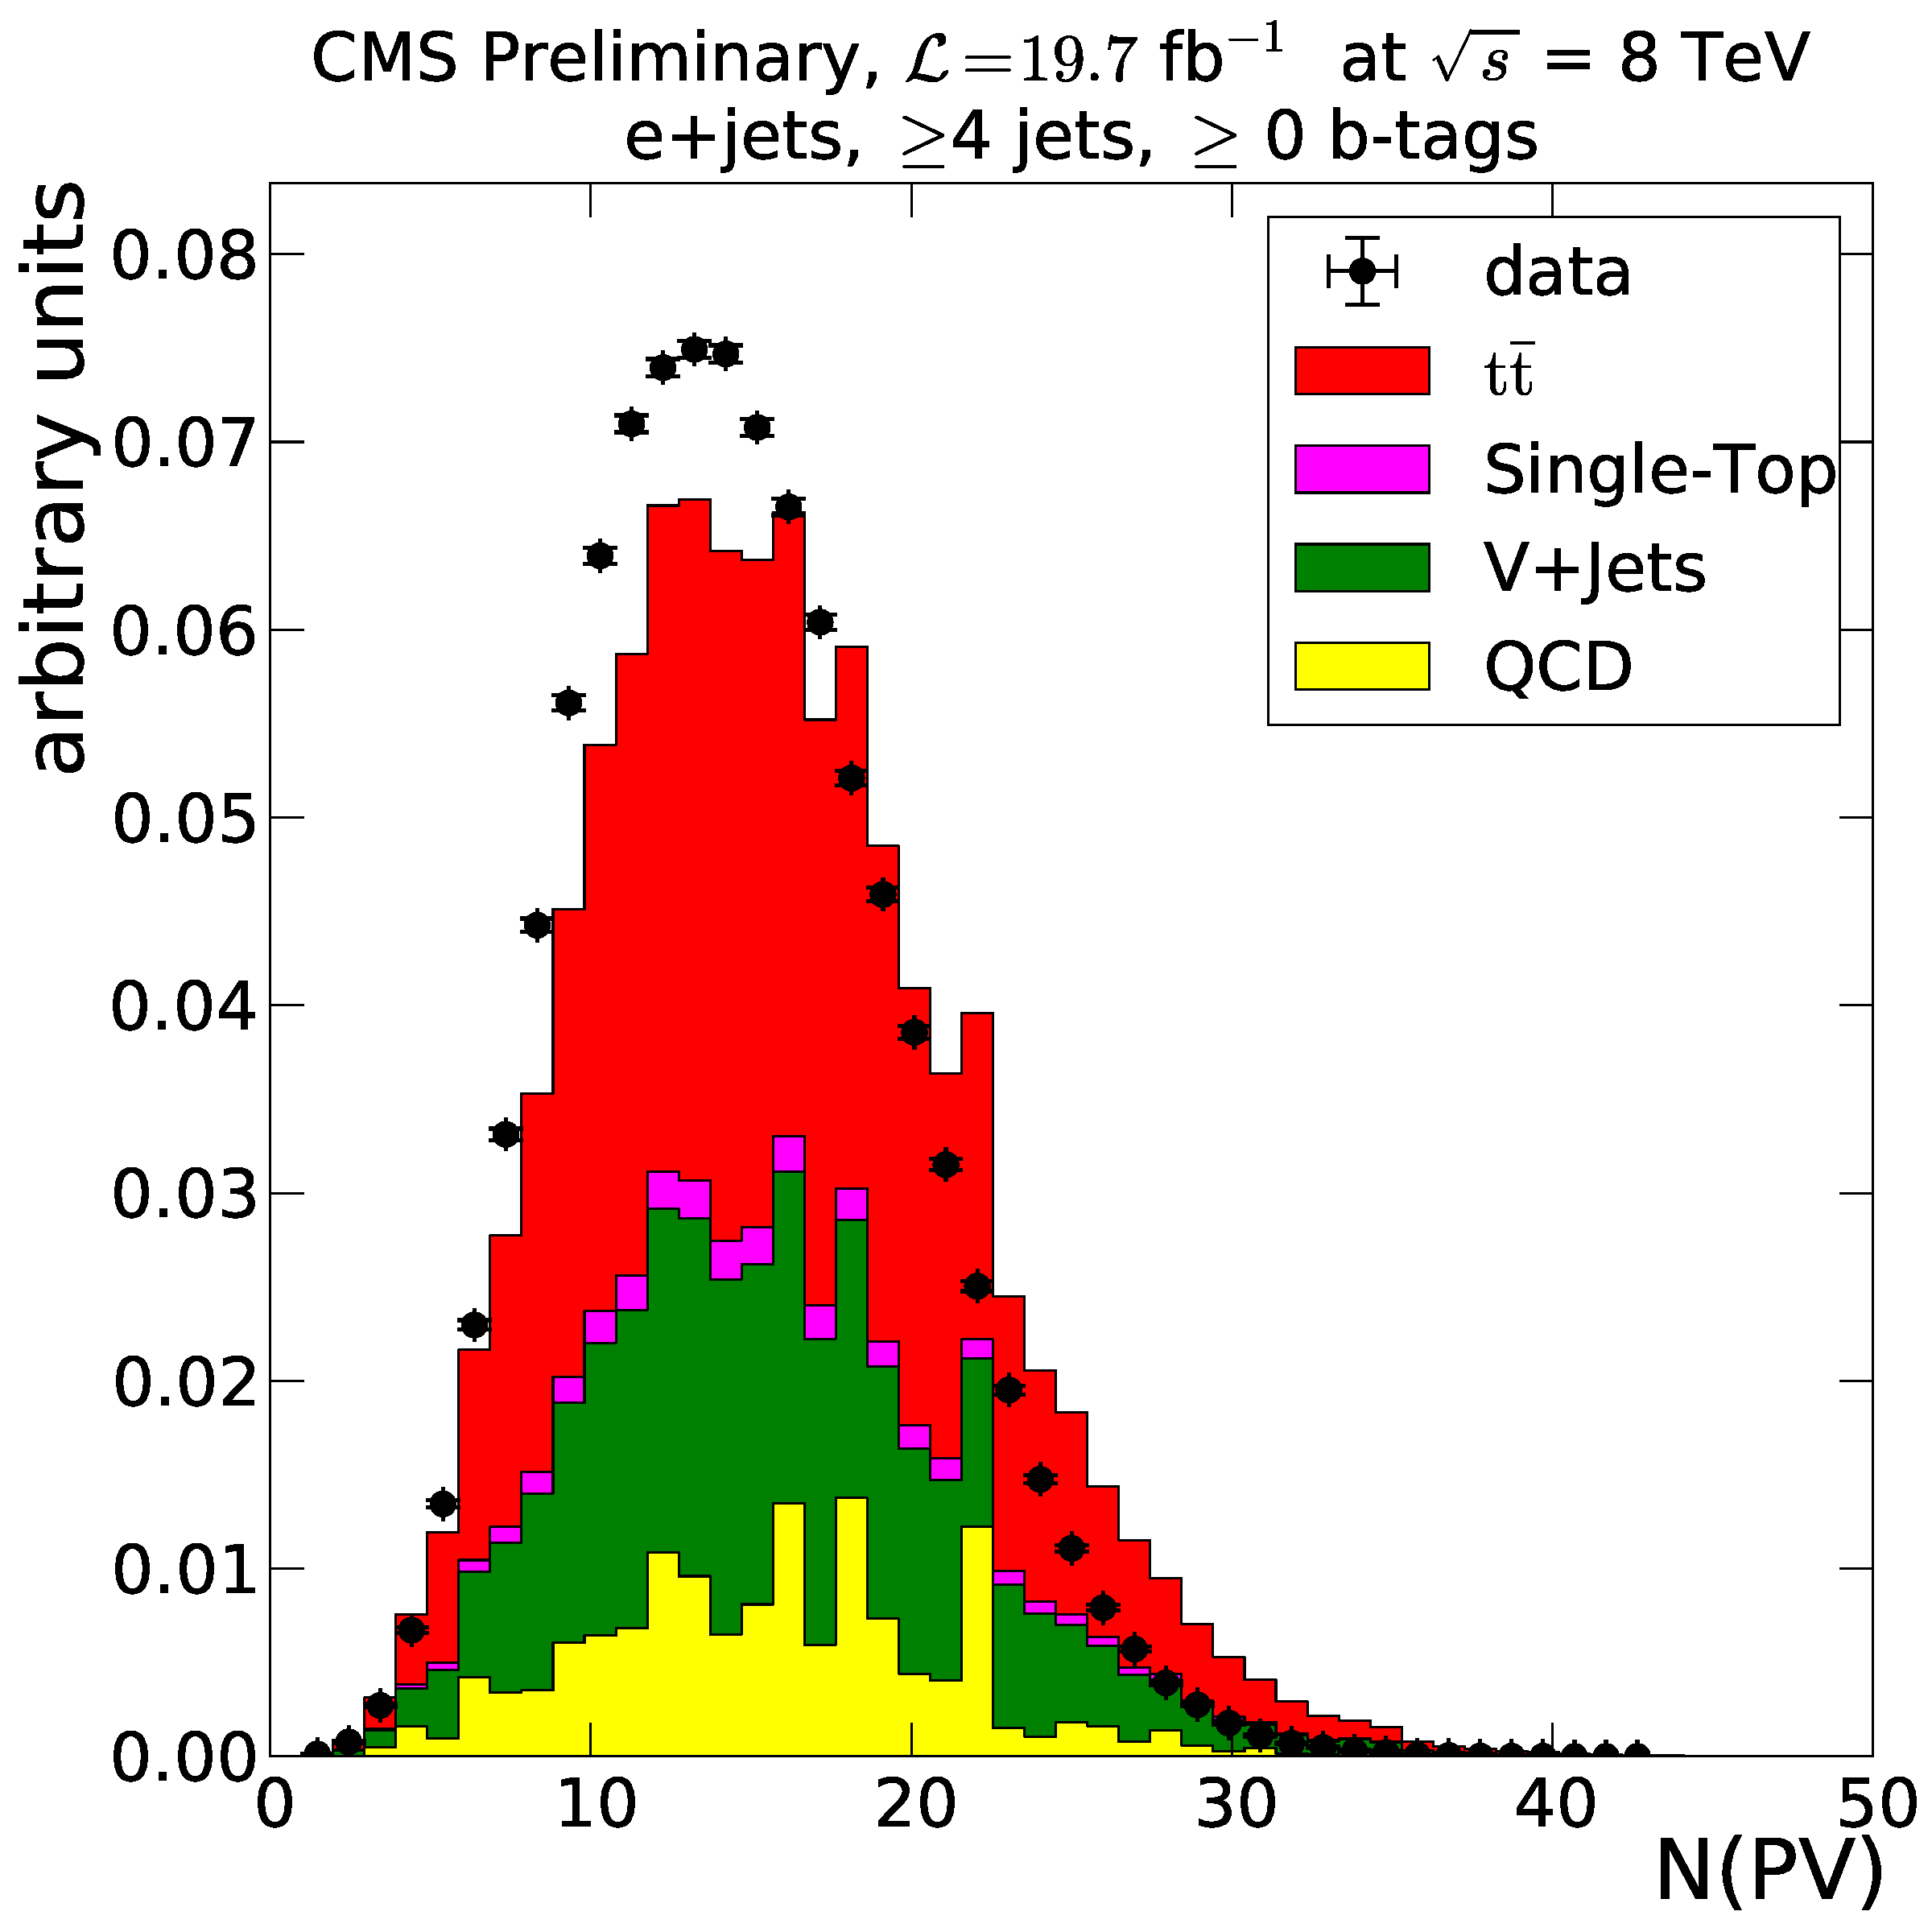
\includegraphics[width=0.50\textwidth]{vertices/EPlusJets_nVertex.pdf}}\hfill
	\subfloat[]{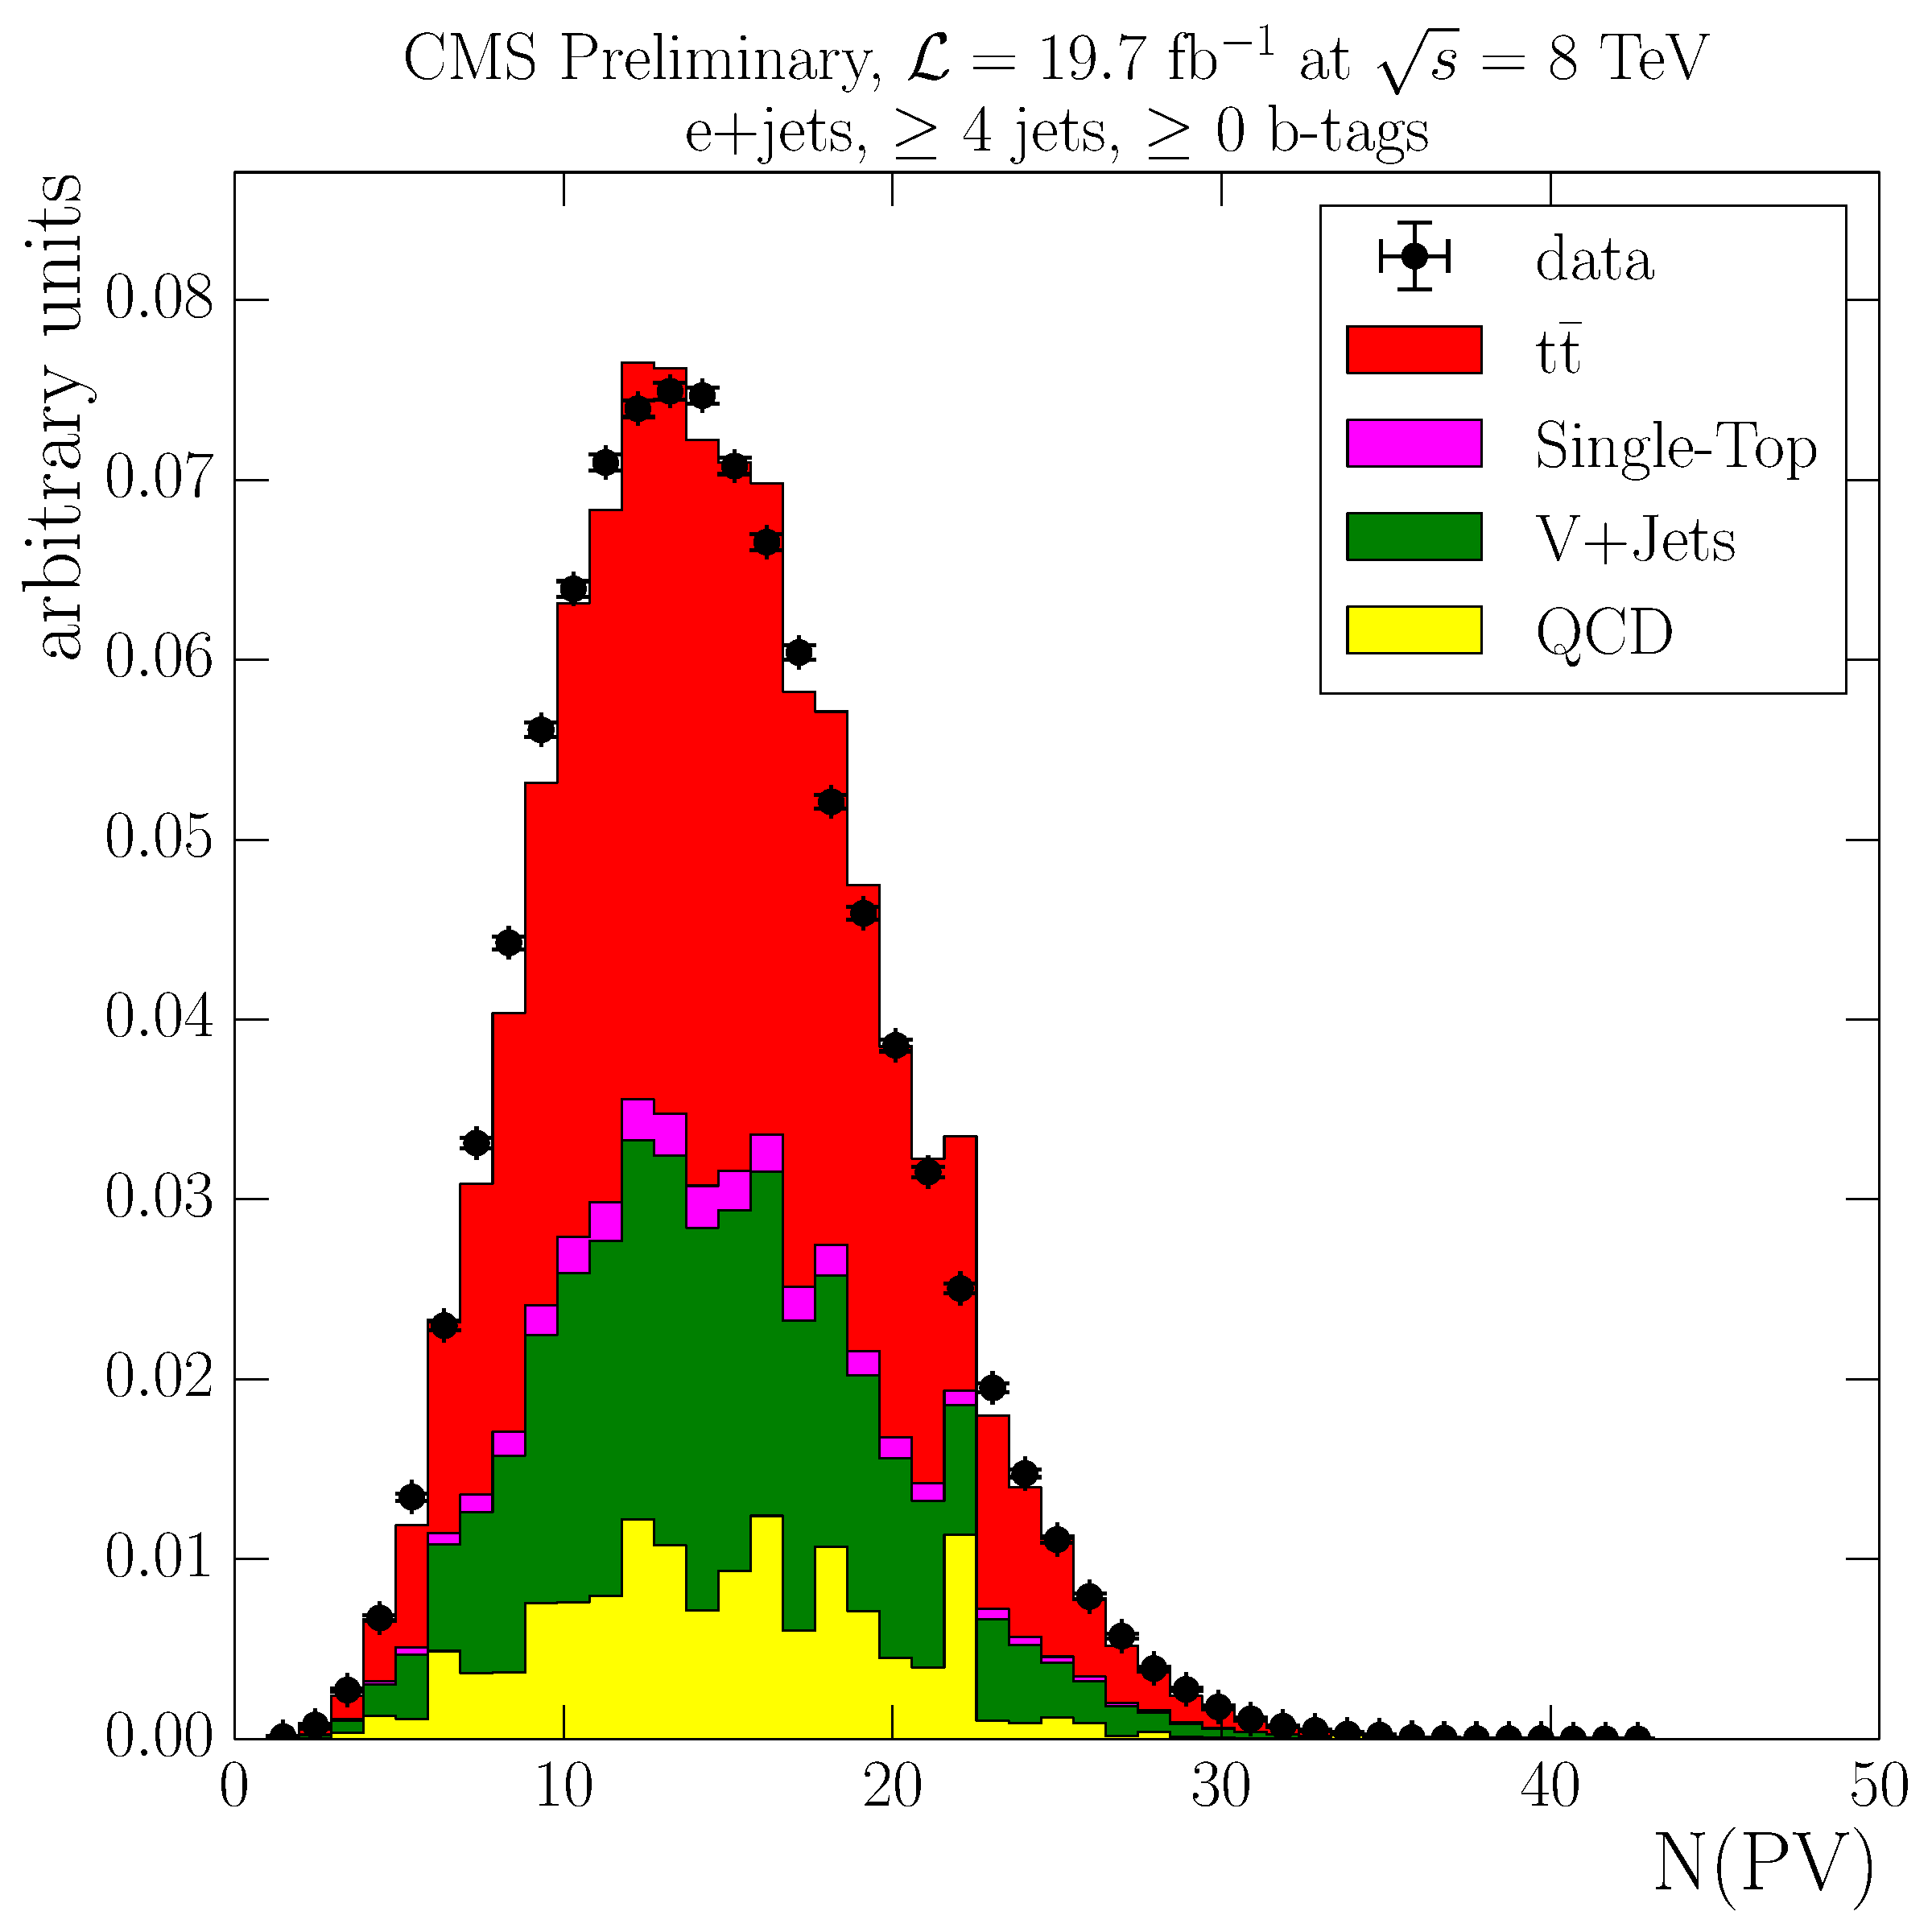
\includegraphics[width=0.50\textwidth]{vertices/EPlusJets_nVertex_reweighted.pdf}} \\
	\subfloat[]{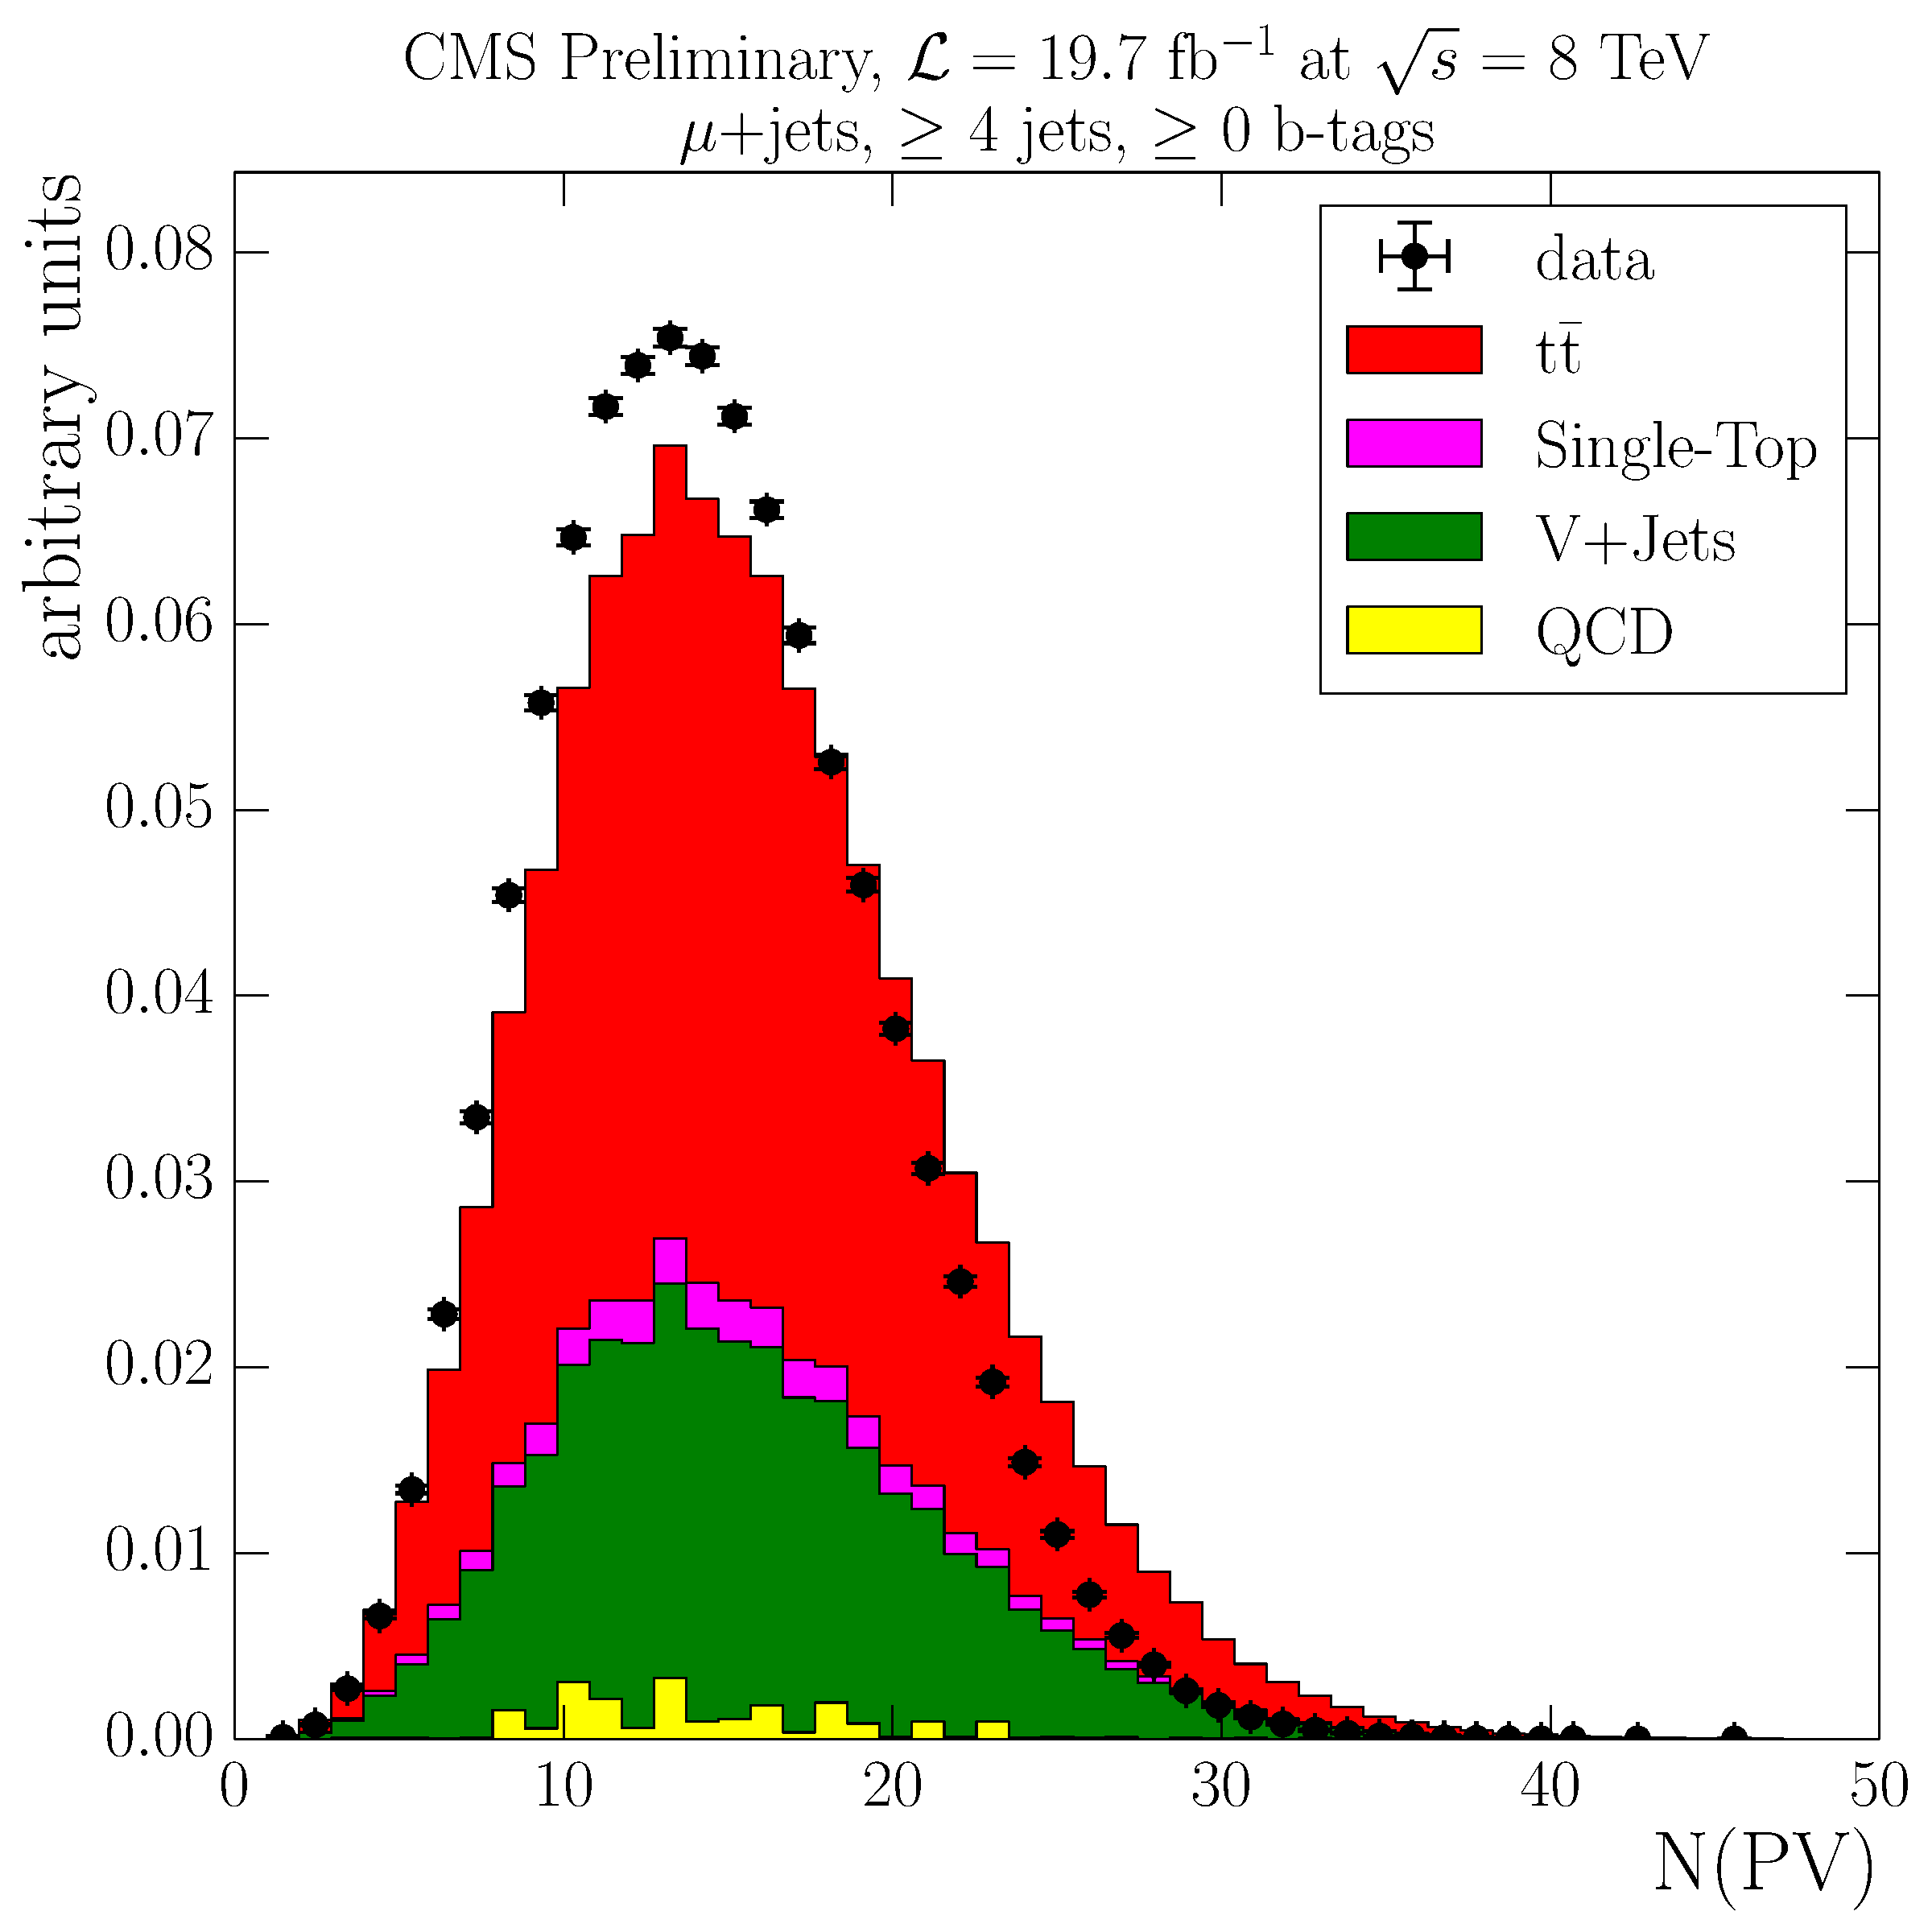
\includegraphics[width=0.50\textwidth]{vertices/MuPlusJets_nVertex.pdf}}\hfill
	\subfloat[]{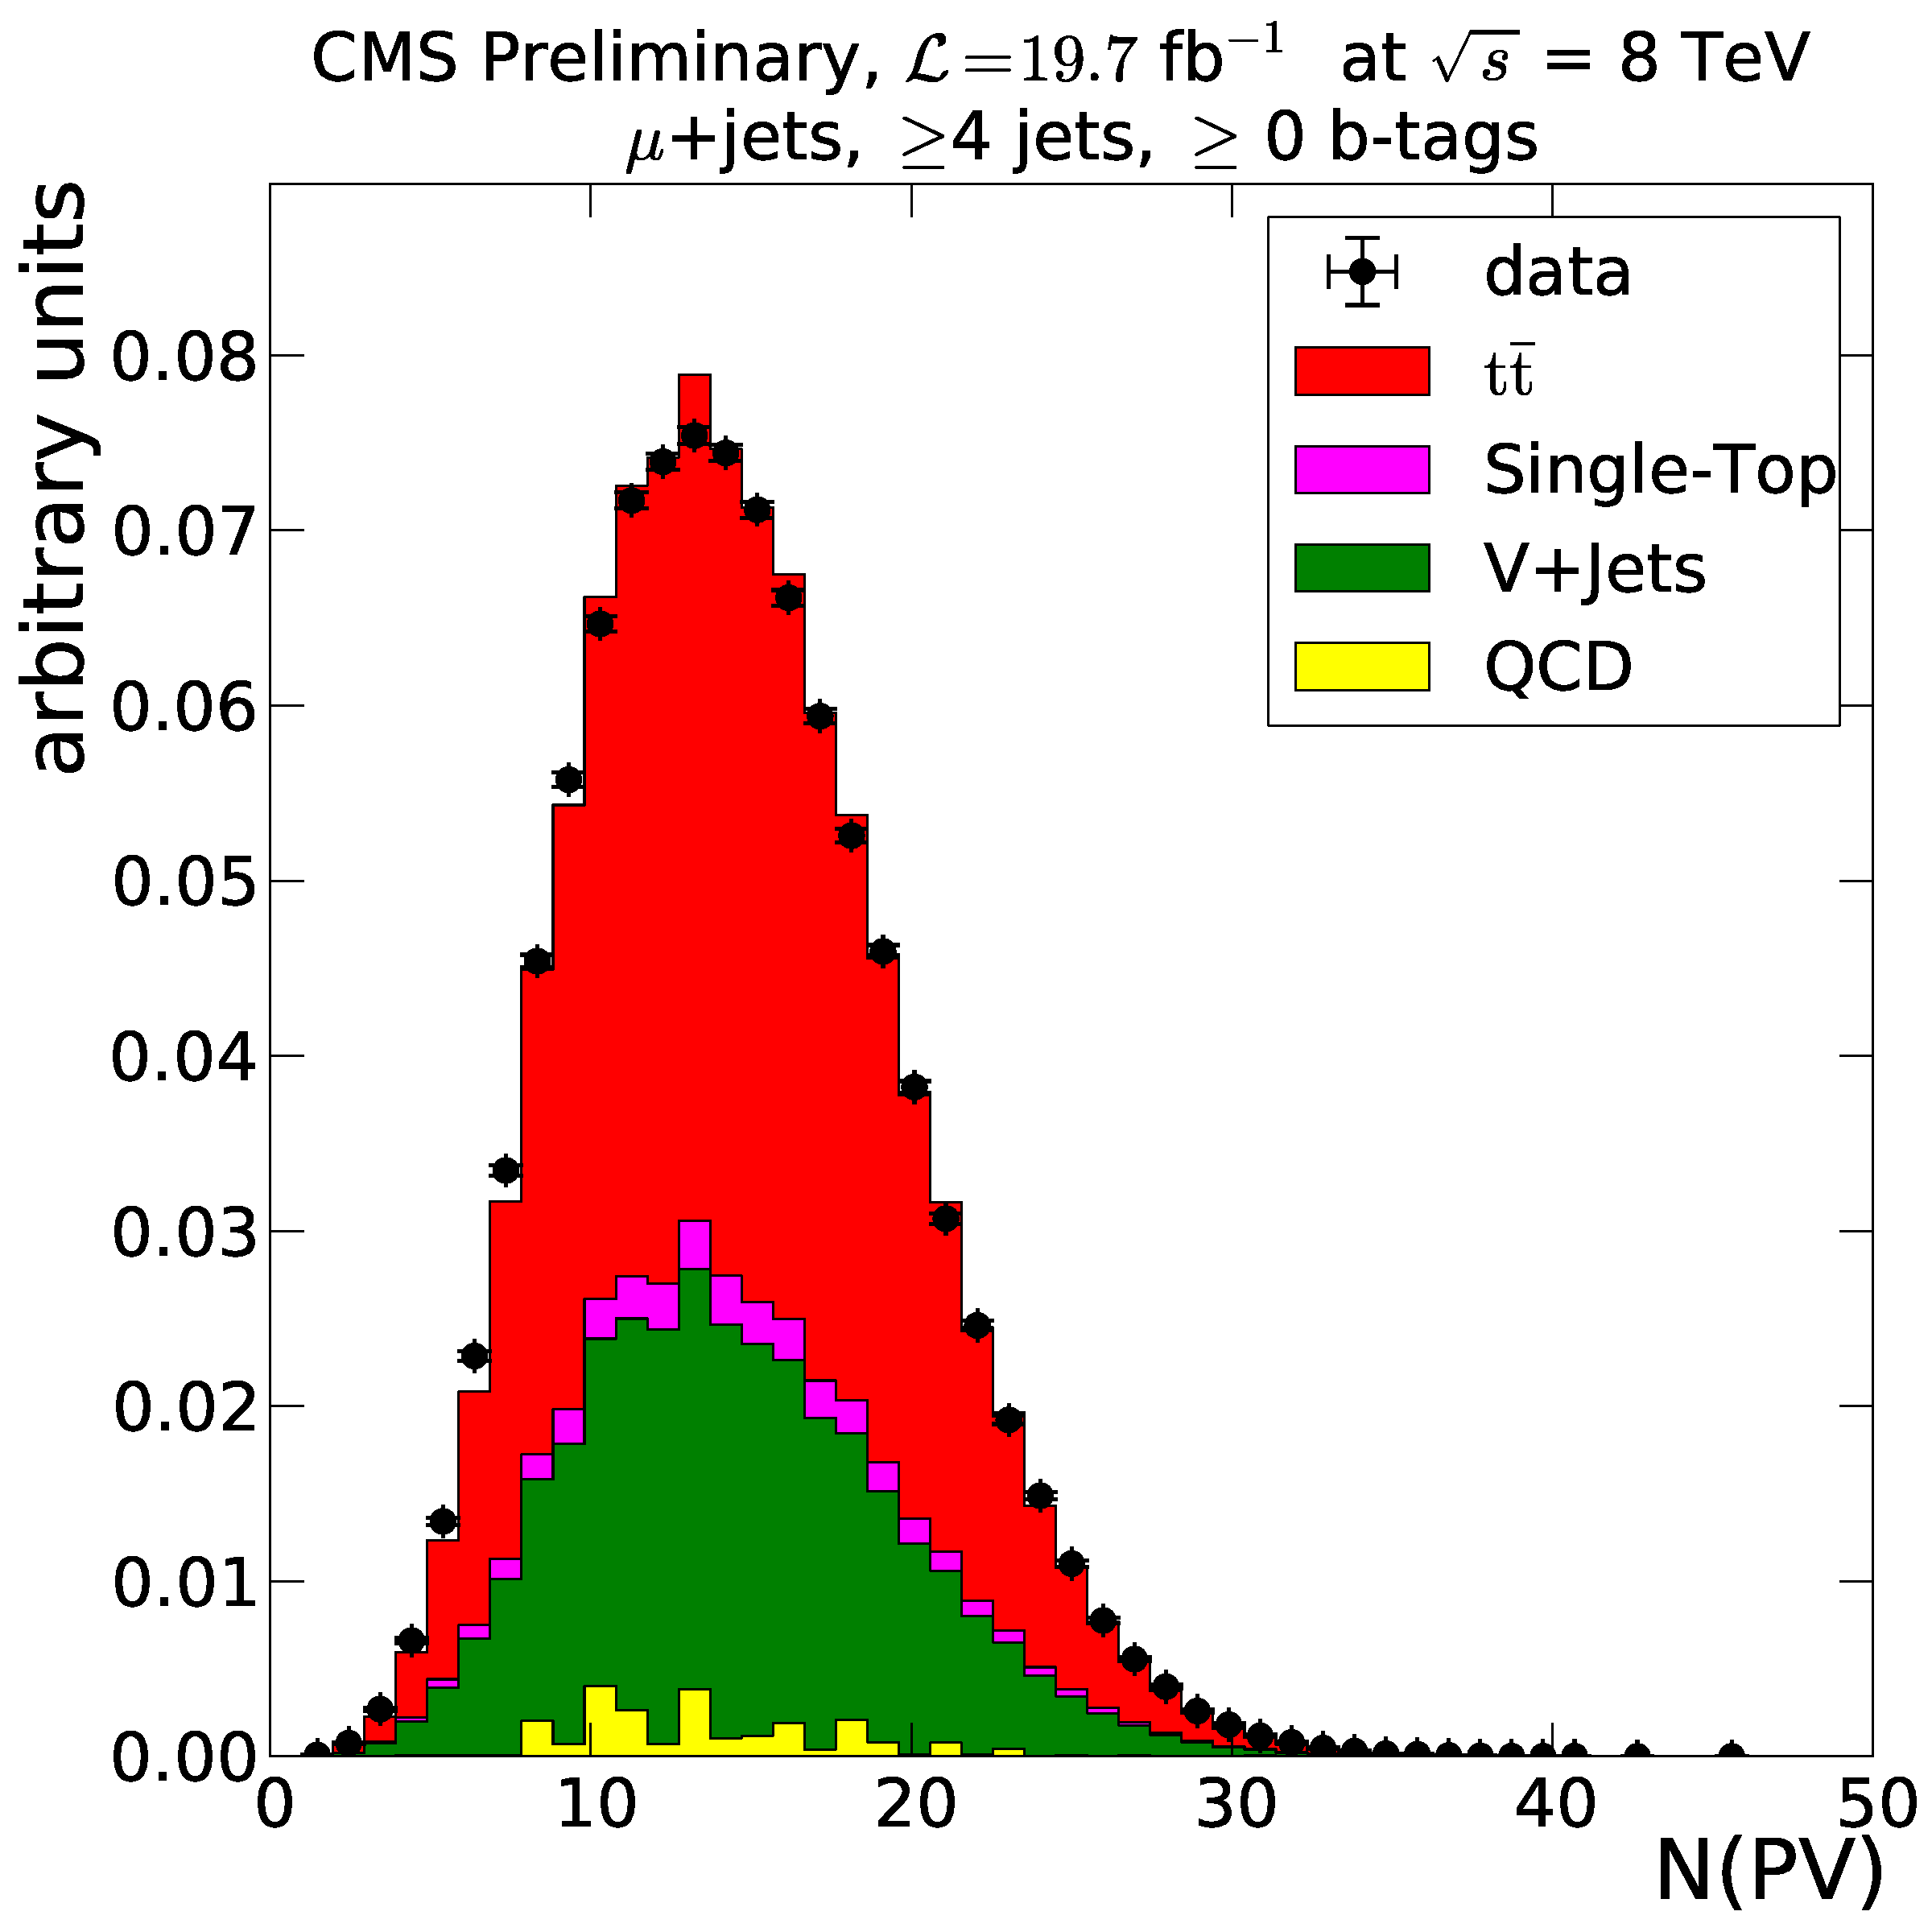
\includegraphics[width=0.50\textwidth]{vertices/MuPlusJets_nVertex_reweighted.pdf}}
    \caption[Number of reconstructed vertices per event before and after pile-up reweighting]{Number of reconstructed
    vertices per event before (left) and after pile-up reweighting (right) in the electron channel (top) and in the muon
    channel (bottom). Both data and sum of the MC samples are normalised to unit area.}
    \label{fig:pileup_vertices}
    %QCD is estimated from MC here. Possible to fix/remove?
\end{figure}

To estimate the number of pile-up vertices in data, the measured instantaneous luminosity in each bunch crossing is
multiplied by an average total inelastic proton-proton cross section. Therefore, two sources of uncertainty arise from
these factors: the luminosity uncertainty, measured to be \SI{4.4}{\pc} by a dedicated study \autocite{CMS_lumi_2012},
and the uncertainty on the total inelastic cross section. To obtain the total cross section value, the CMS measurement
of \SI{68\pm4.5}{\milli\barn} based on \SI{7}{\TeV} data \autocite{CMS_total_inelastic_7TeV} was extrapolated to the
\SI{8}{\TeV} value of \SI{69.3}{\milli\barn}. The recommended uncertainty on this value, set to be \SI{5}{\pc}, covers
the modelling and physics aspects of pile-up simulation that have not been fully studied to date.

%https://twiki.cern.ch/twiki/bin/viewauth/CMS/PileupSystematicErrors (this has been updated to 69.4mb!)

The effect of the \SI{\pm5}{\pc} variations in total inelastic cross section on the estimate of the true number of
vertices in data is shown in Figure~\ref{fig:pileup_truth}, whereas its effect on the simulated distributions is shown
in Figure~\ref{fig:pileup_vertices_variations} for both electron and muon channels.

 \begin{figure}[htbp]
   	\centering
    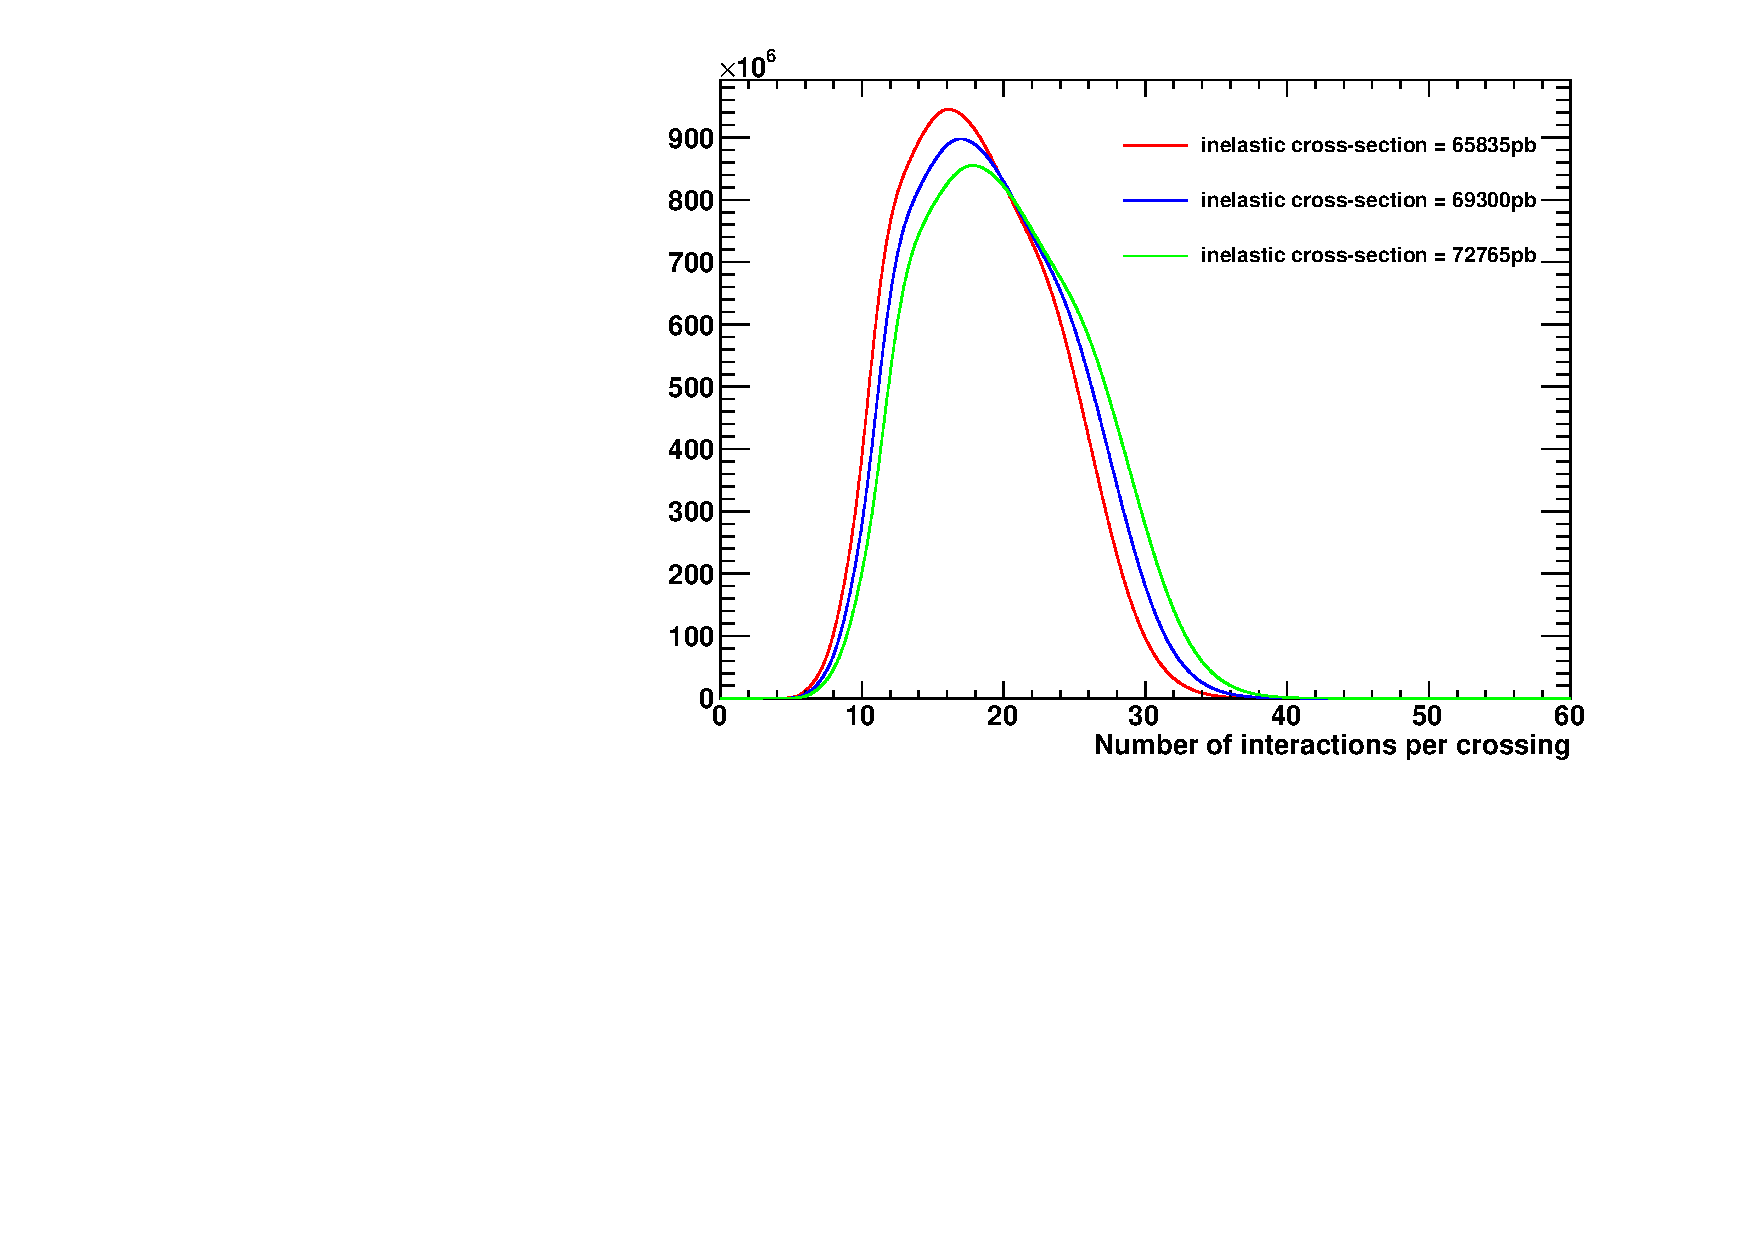
\includegraphics[width=0.77\textwidth]{vertices/PileUp_2012_truth_data.pdf}
    \caption[Number of expected vertices per event for central and $\pm1\sigma$ variations of the total inelastic cross
    section for the 2012 data]{Number of expected vertices per event for central and $\pm1\sigma$ variations of the
    total inelastic cross section for the 2012 data.}
    \label{fig:pileup_truth}
 \end{figure}

\begin{figure}[!htpb]
	\centering
	\subfloat[]{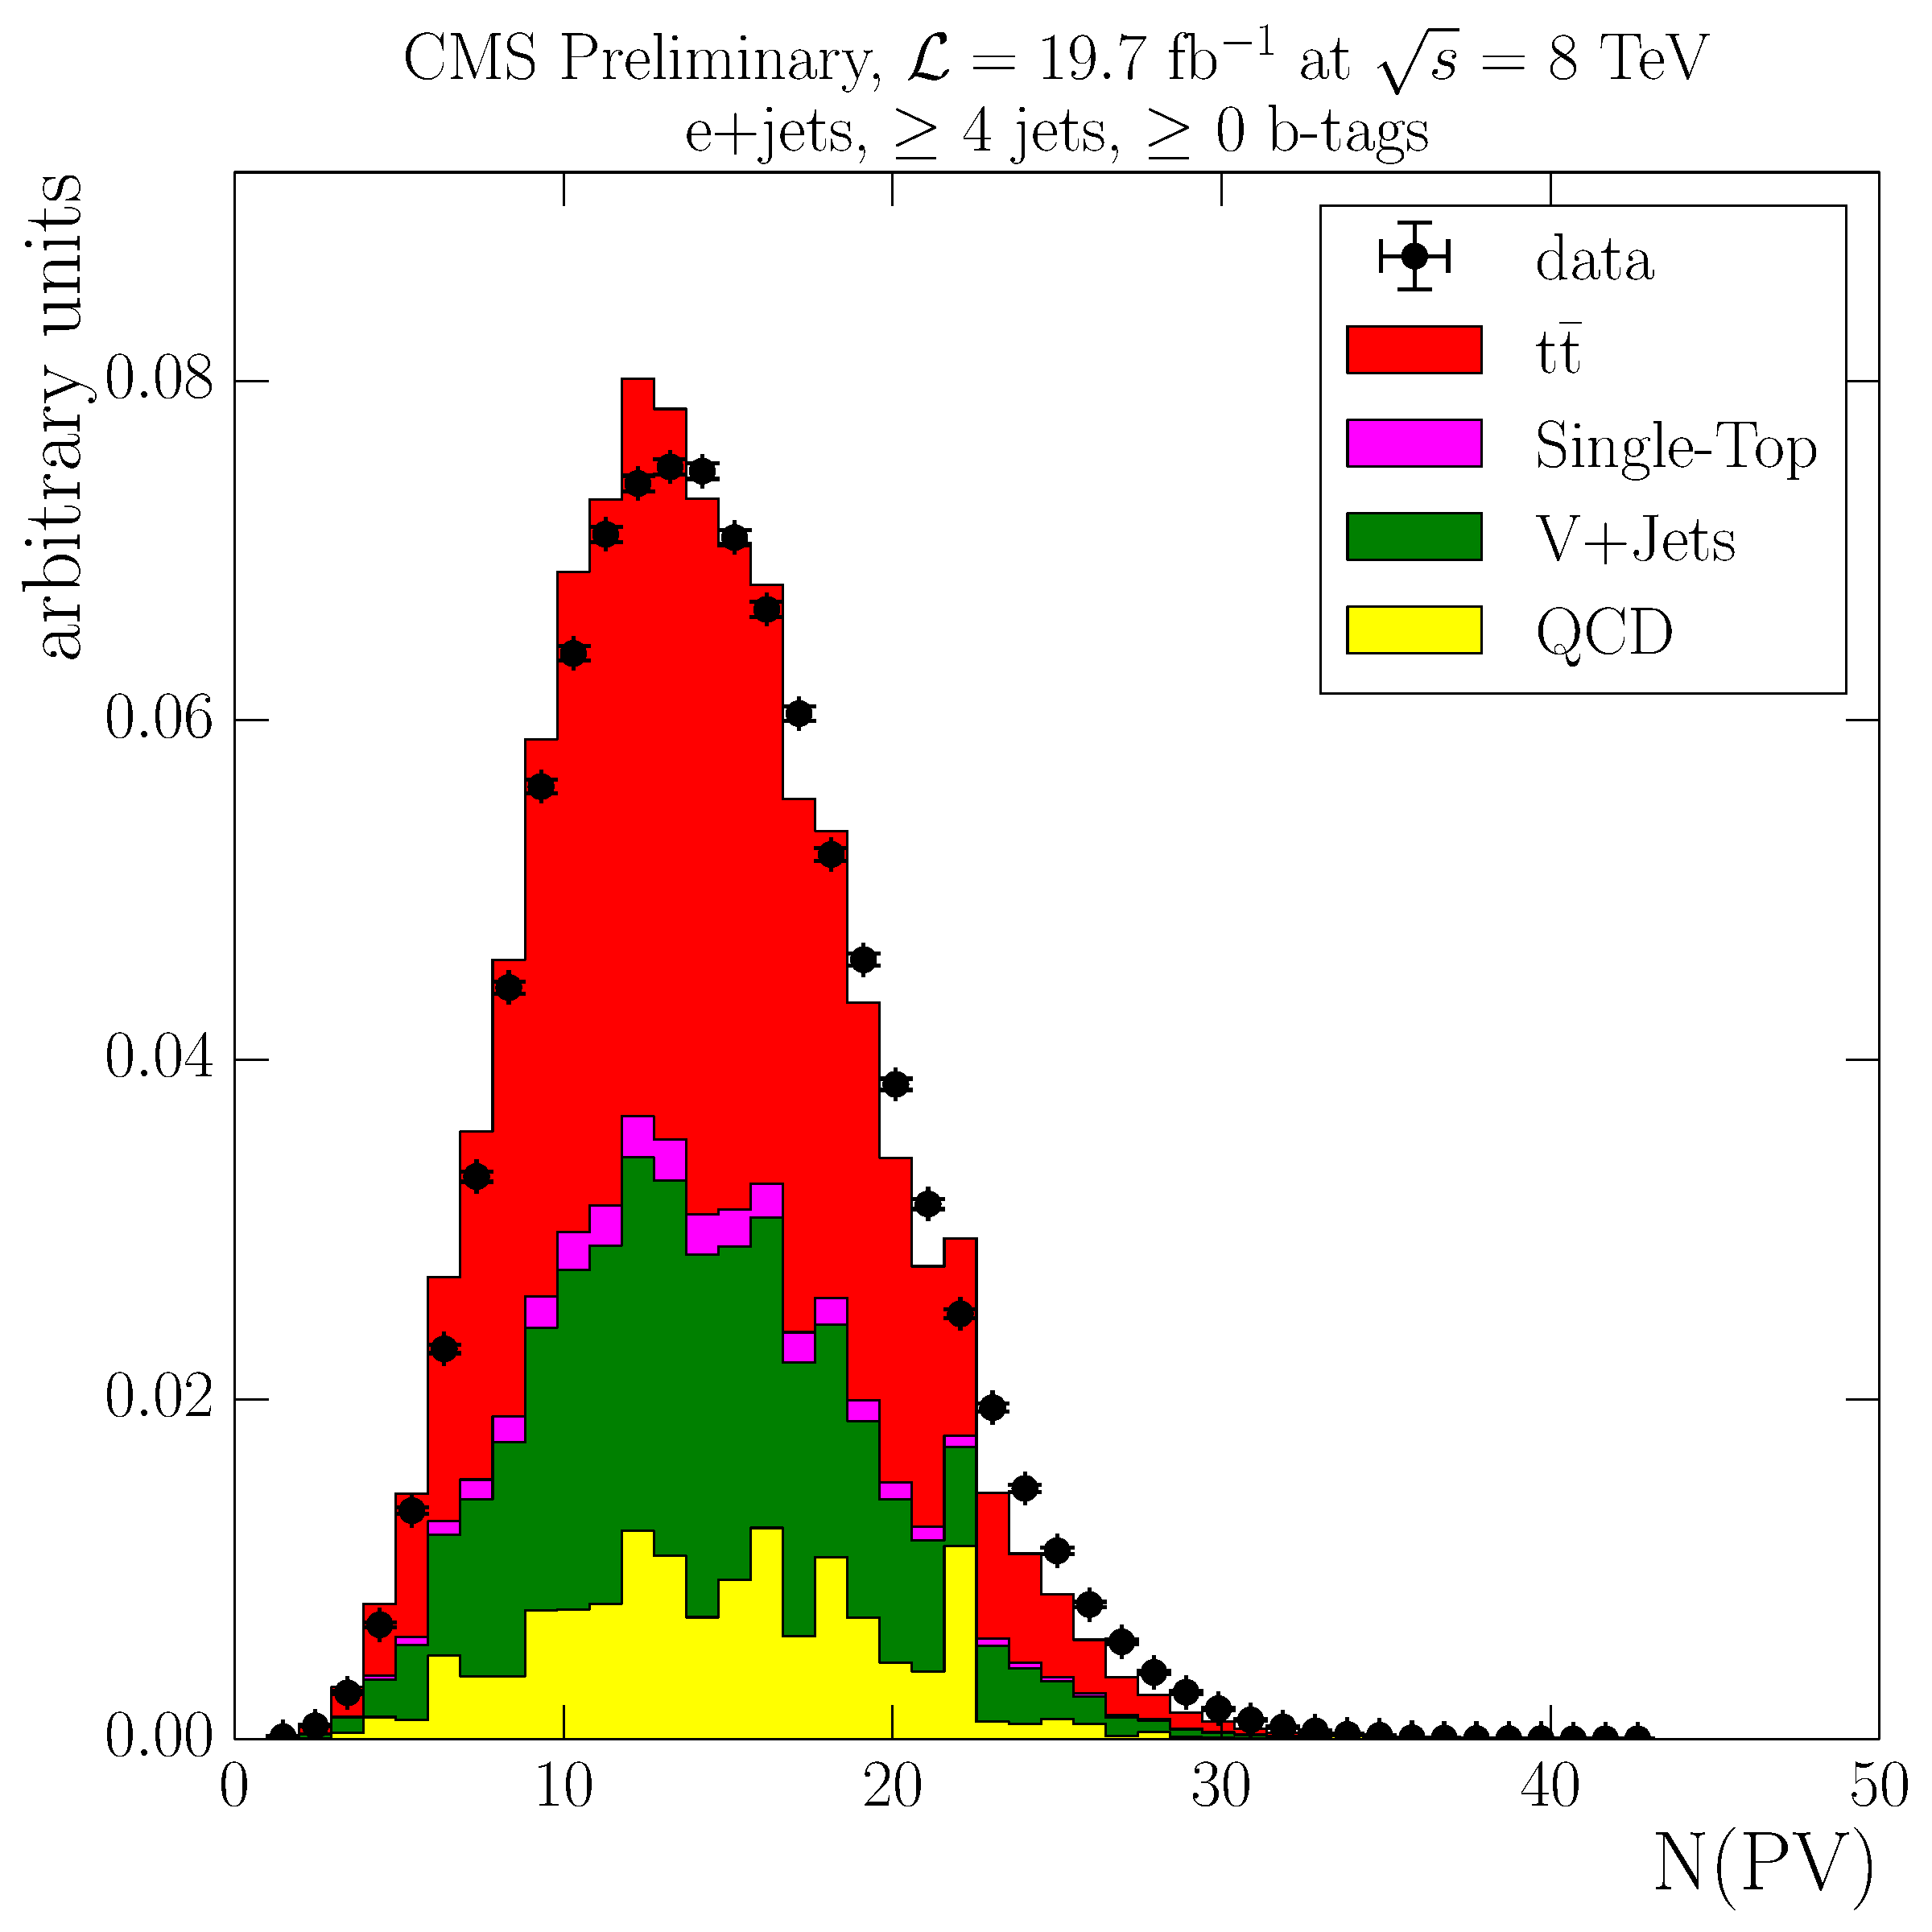
\includegraphics[width=0.50\textwidth]{vertices/EPlusJets_nVertex_reweighted_PU_down.pdf}}\hfill
	\subfloat[]{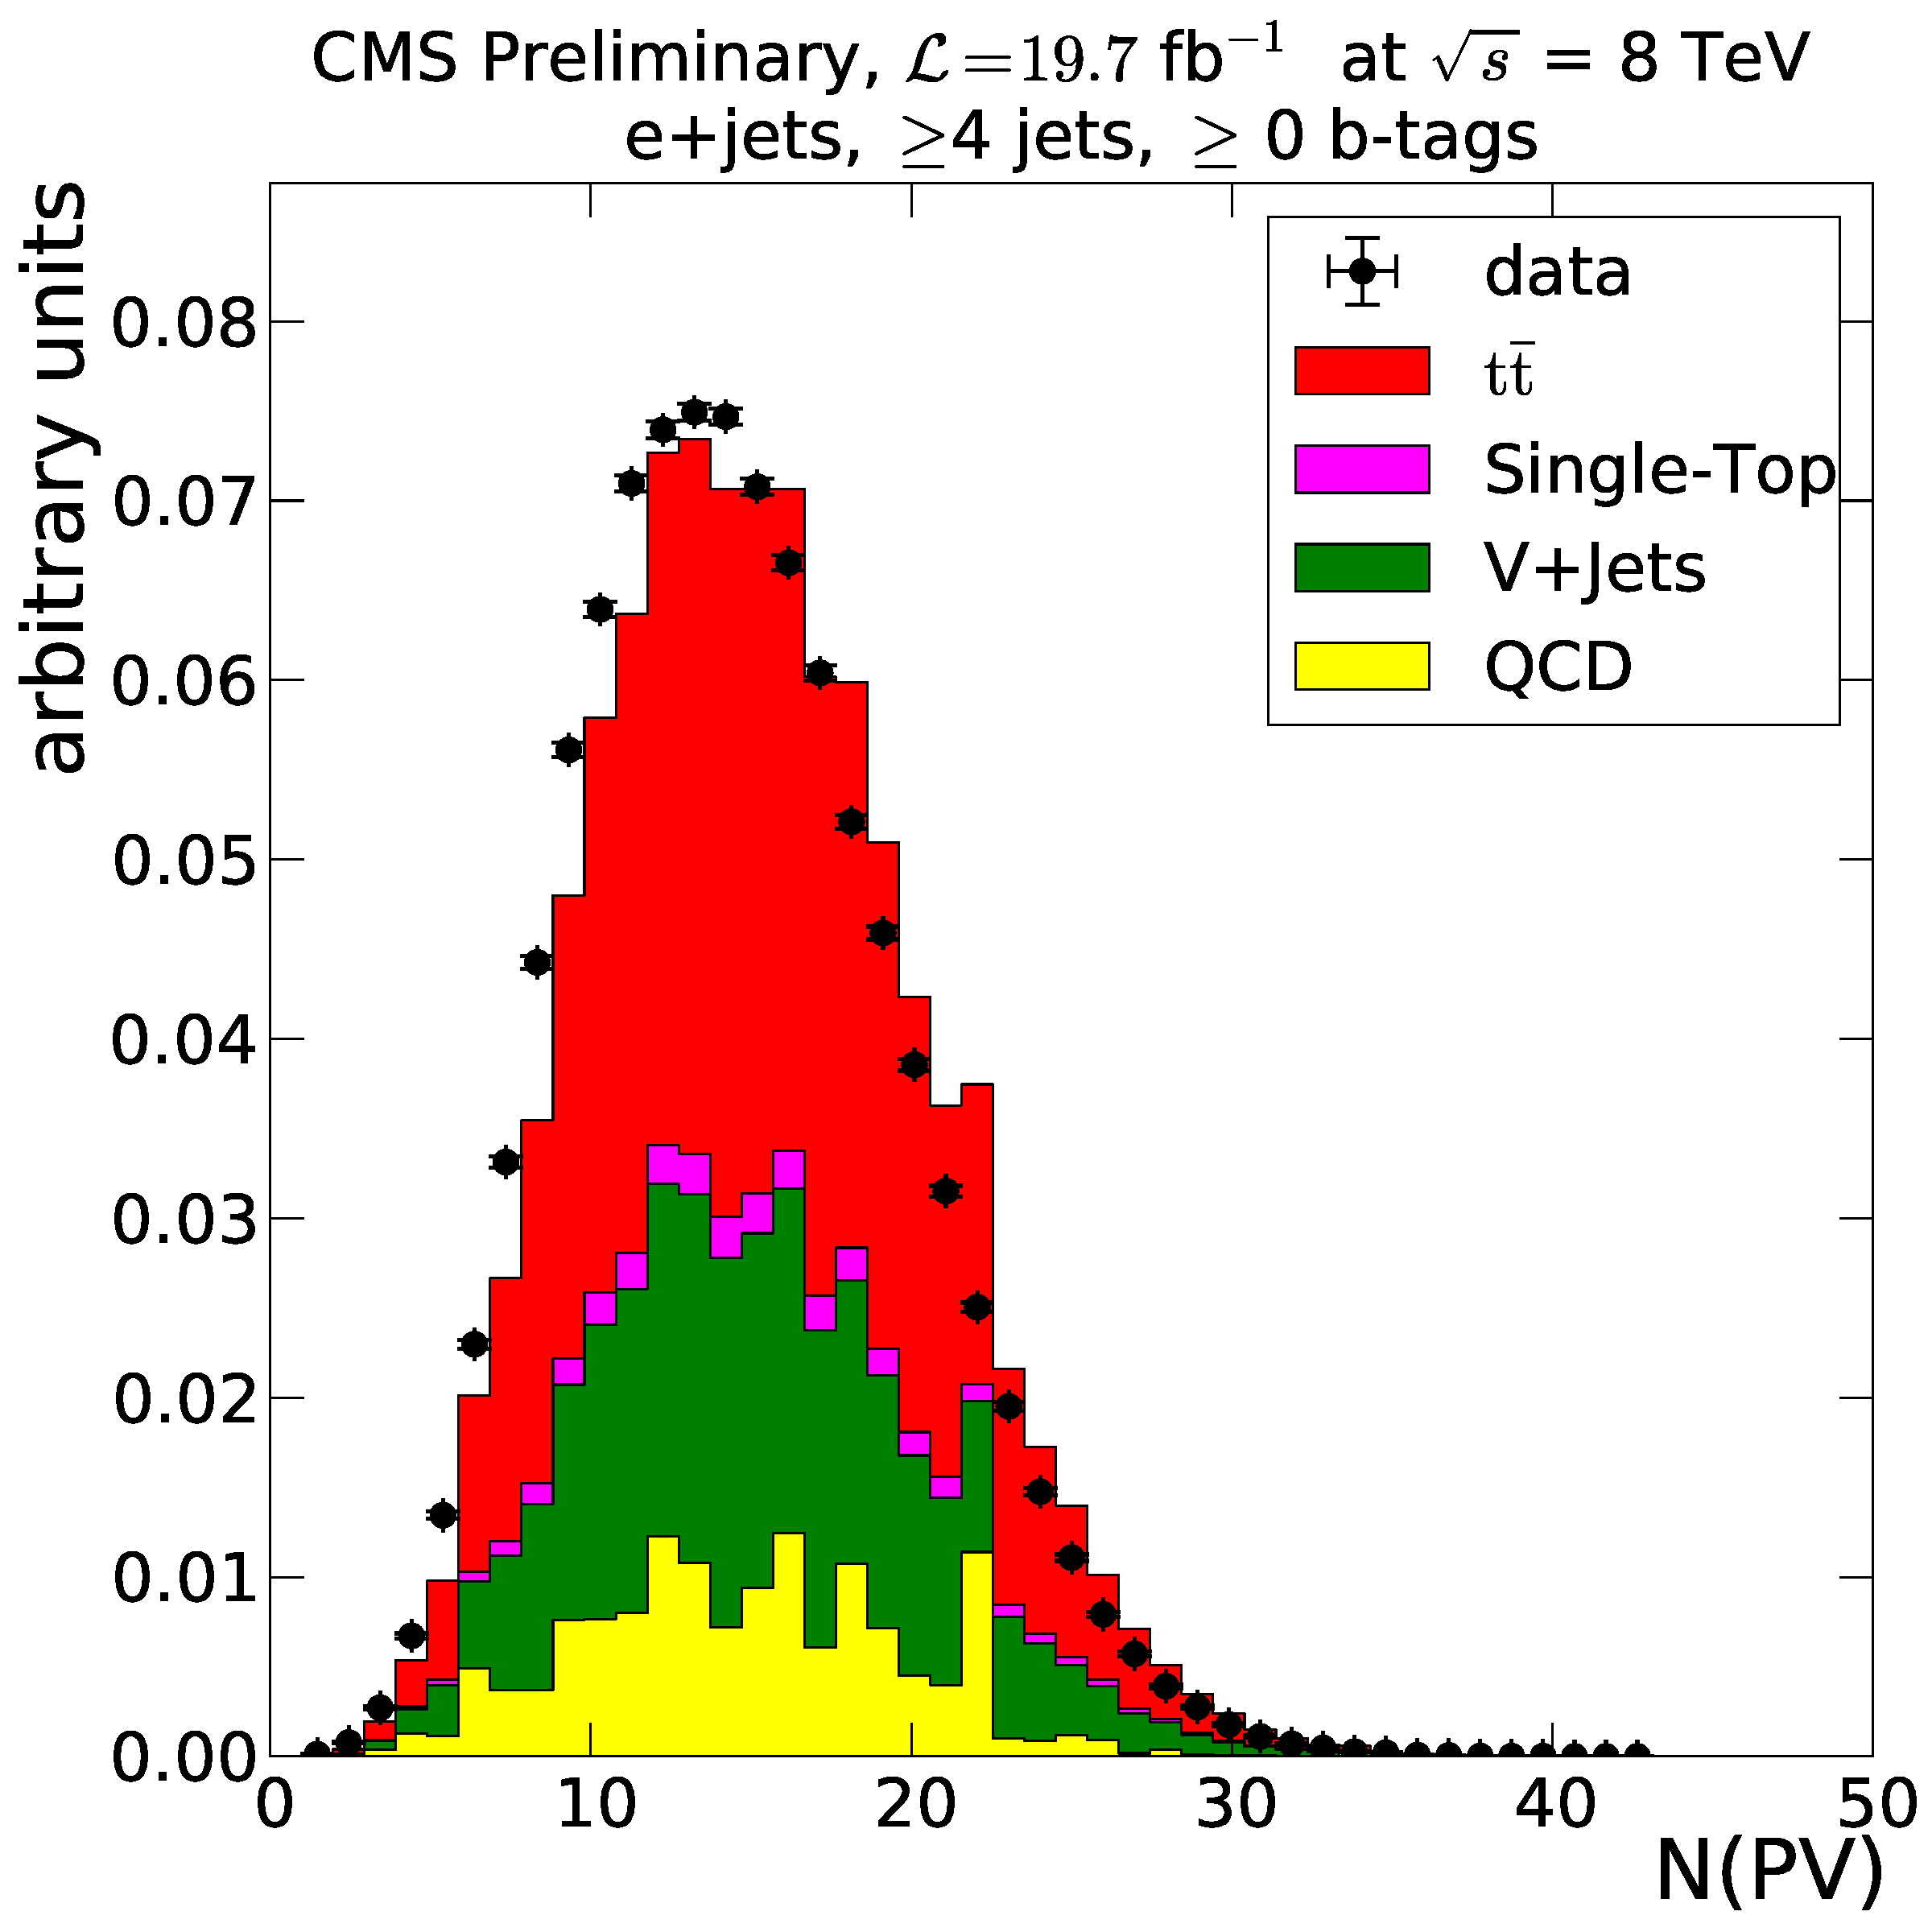
\includegraphics[width=0.50\textwidth]{vertices/EPlusJets_nVertex_reweighted_PU_up.pdf}} \\
	\subfloat[]{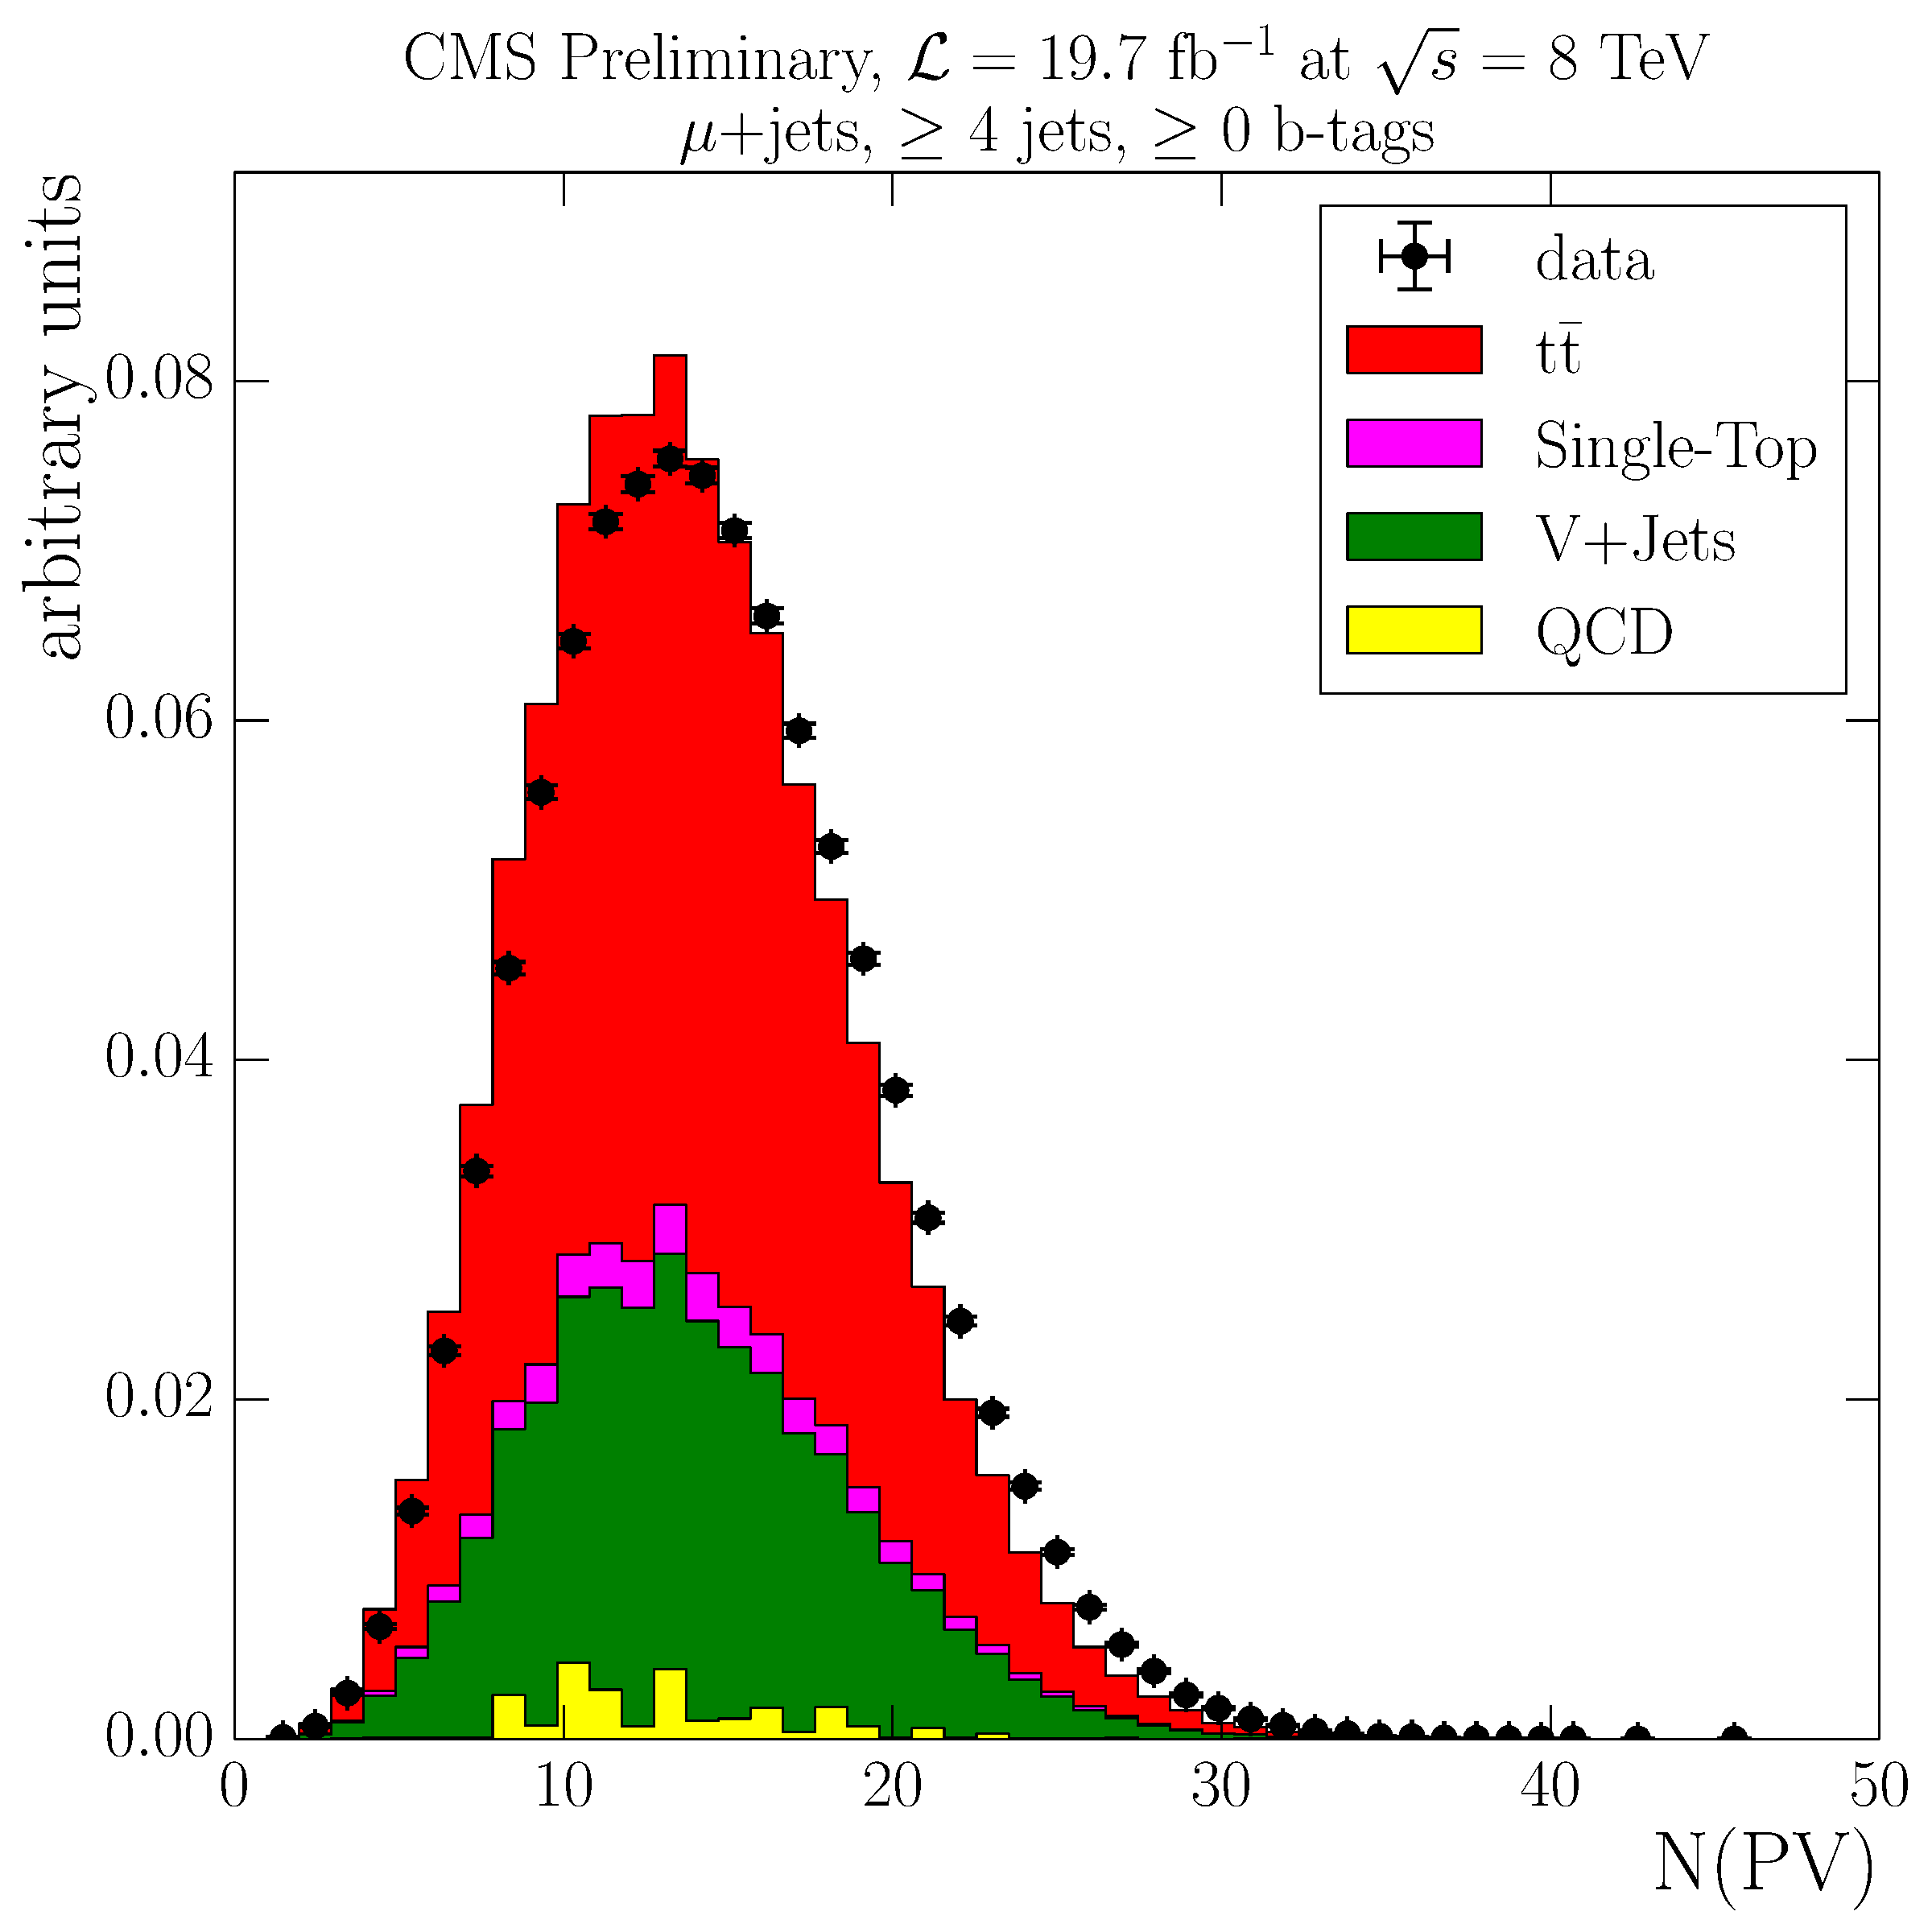
\includegraphics[width=0.50\textwidth]{vertices/MuPlusJets_nVertex_reweighted_PU_down.pdf}}\hfill
	\subfloat[]{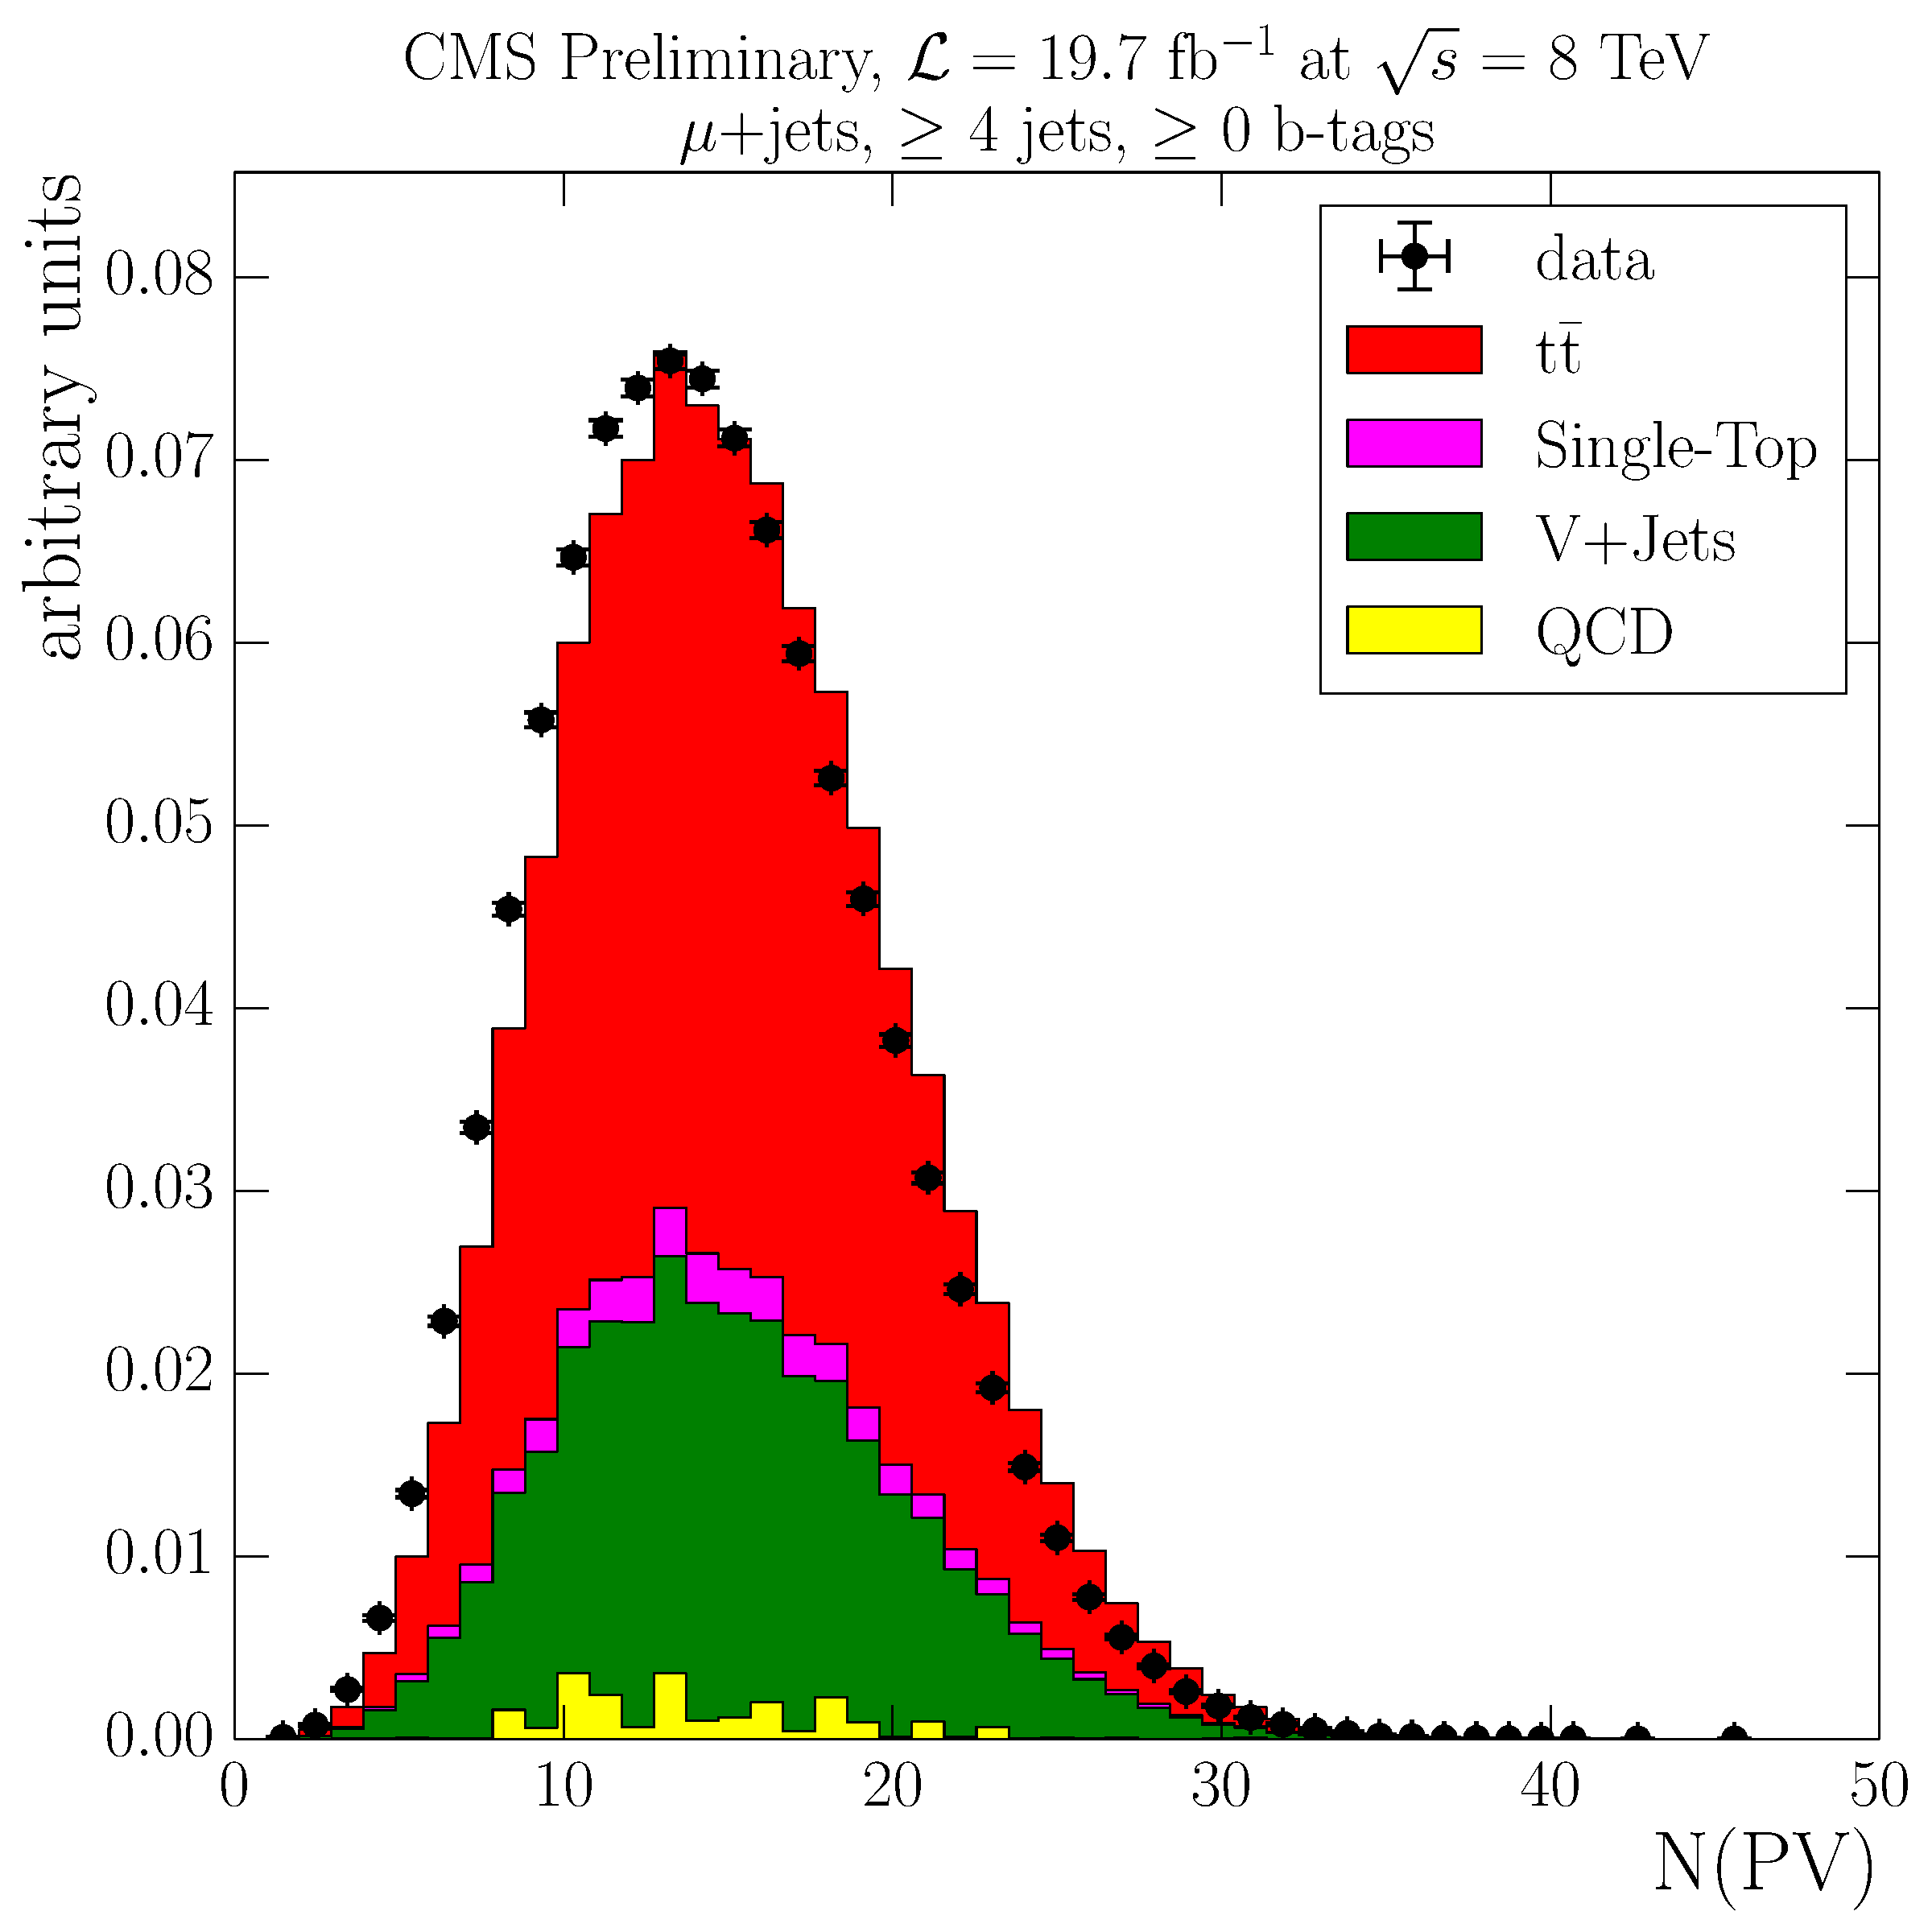
\includegraphics[width=0.50\textwidth]{vertices/MuPlusJets_nVertex_reweighted_PU_up.pdf}}
    \caption[Number of reconstructed vertices per event for $\pm1\sigma$ variations of the pile-up reweighting
    procedure]{Number of reconstructed vertices per event for $-1\sigma$ (left) and $+1\sigma$ variation (right) of the
    pile-up reweighting procedure for the electron channel (top) and the muon channel (bottom).}
    \label{fig:pileup_vertices_variations}
\end{figure}


\subsection{b-tagging corrections}
\label{ss_xsection:btagging_corrections}
In order to mitigate the background (QCD in particular), b-tagging is applied in the event selection of this analysis.
Similarly to the top quark mass analysis, the CSV algorithm with the medium working point providing
\SI{\sim70}{\percent} efficiency and \SI{\sim1}{\percent} mis-tag rate (Section~\ref{sss:b-tagging}) was used. However,
in contrast with the 2011 analysis where the b-tagging corrections were implemented in the construction of the event
likelihood, in this work scale factors are applied to Monte Carlo events. This is done in order to correct for the
mismatch between the algorithm efficiency seen in data and MC \autocite{btagging_CMS_8TeV_results}. \pt and
$\eta$-dependent scale factors were derived by the CMS b-tag Physics Object Group \autocite{btag_weights_2011} and are
used to reweight the simulated events. The overall jet content of the event is taken into account, such as the number of
jets originating from light and heavy quarks.

\begin{figure}[!htpb]
	\centering
	\subfloat[]{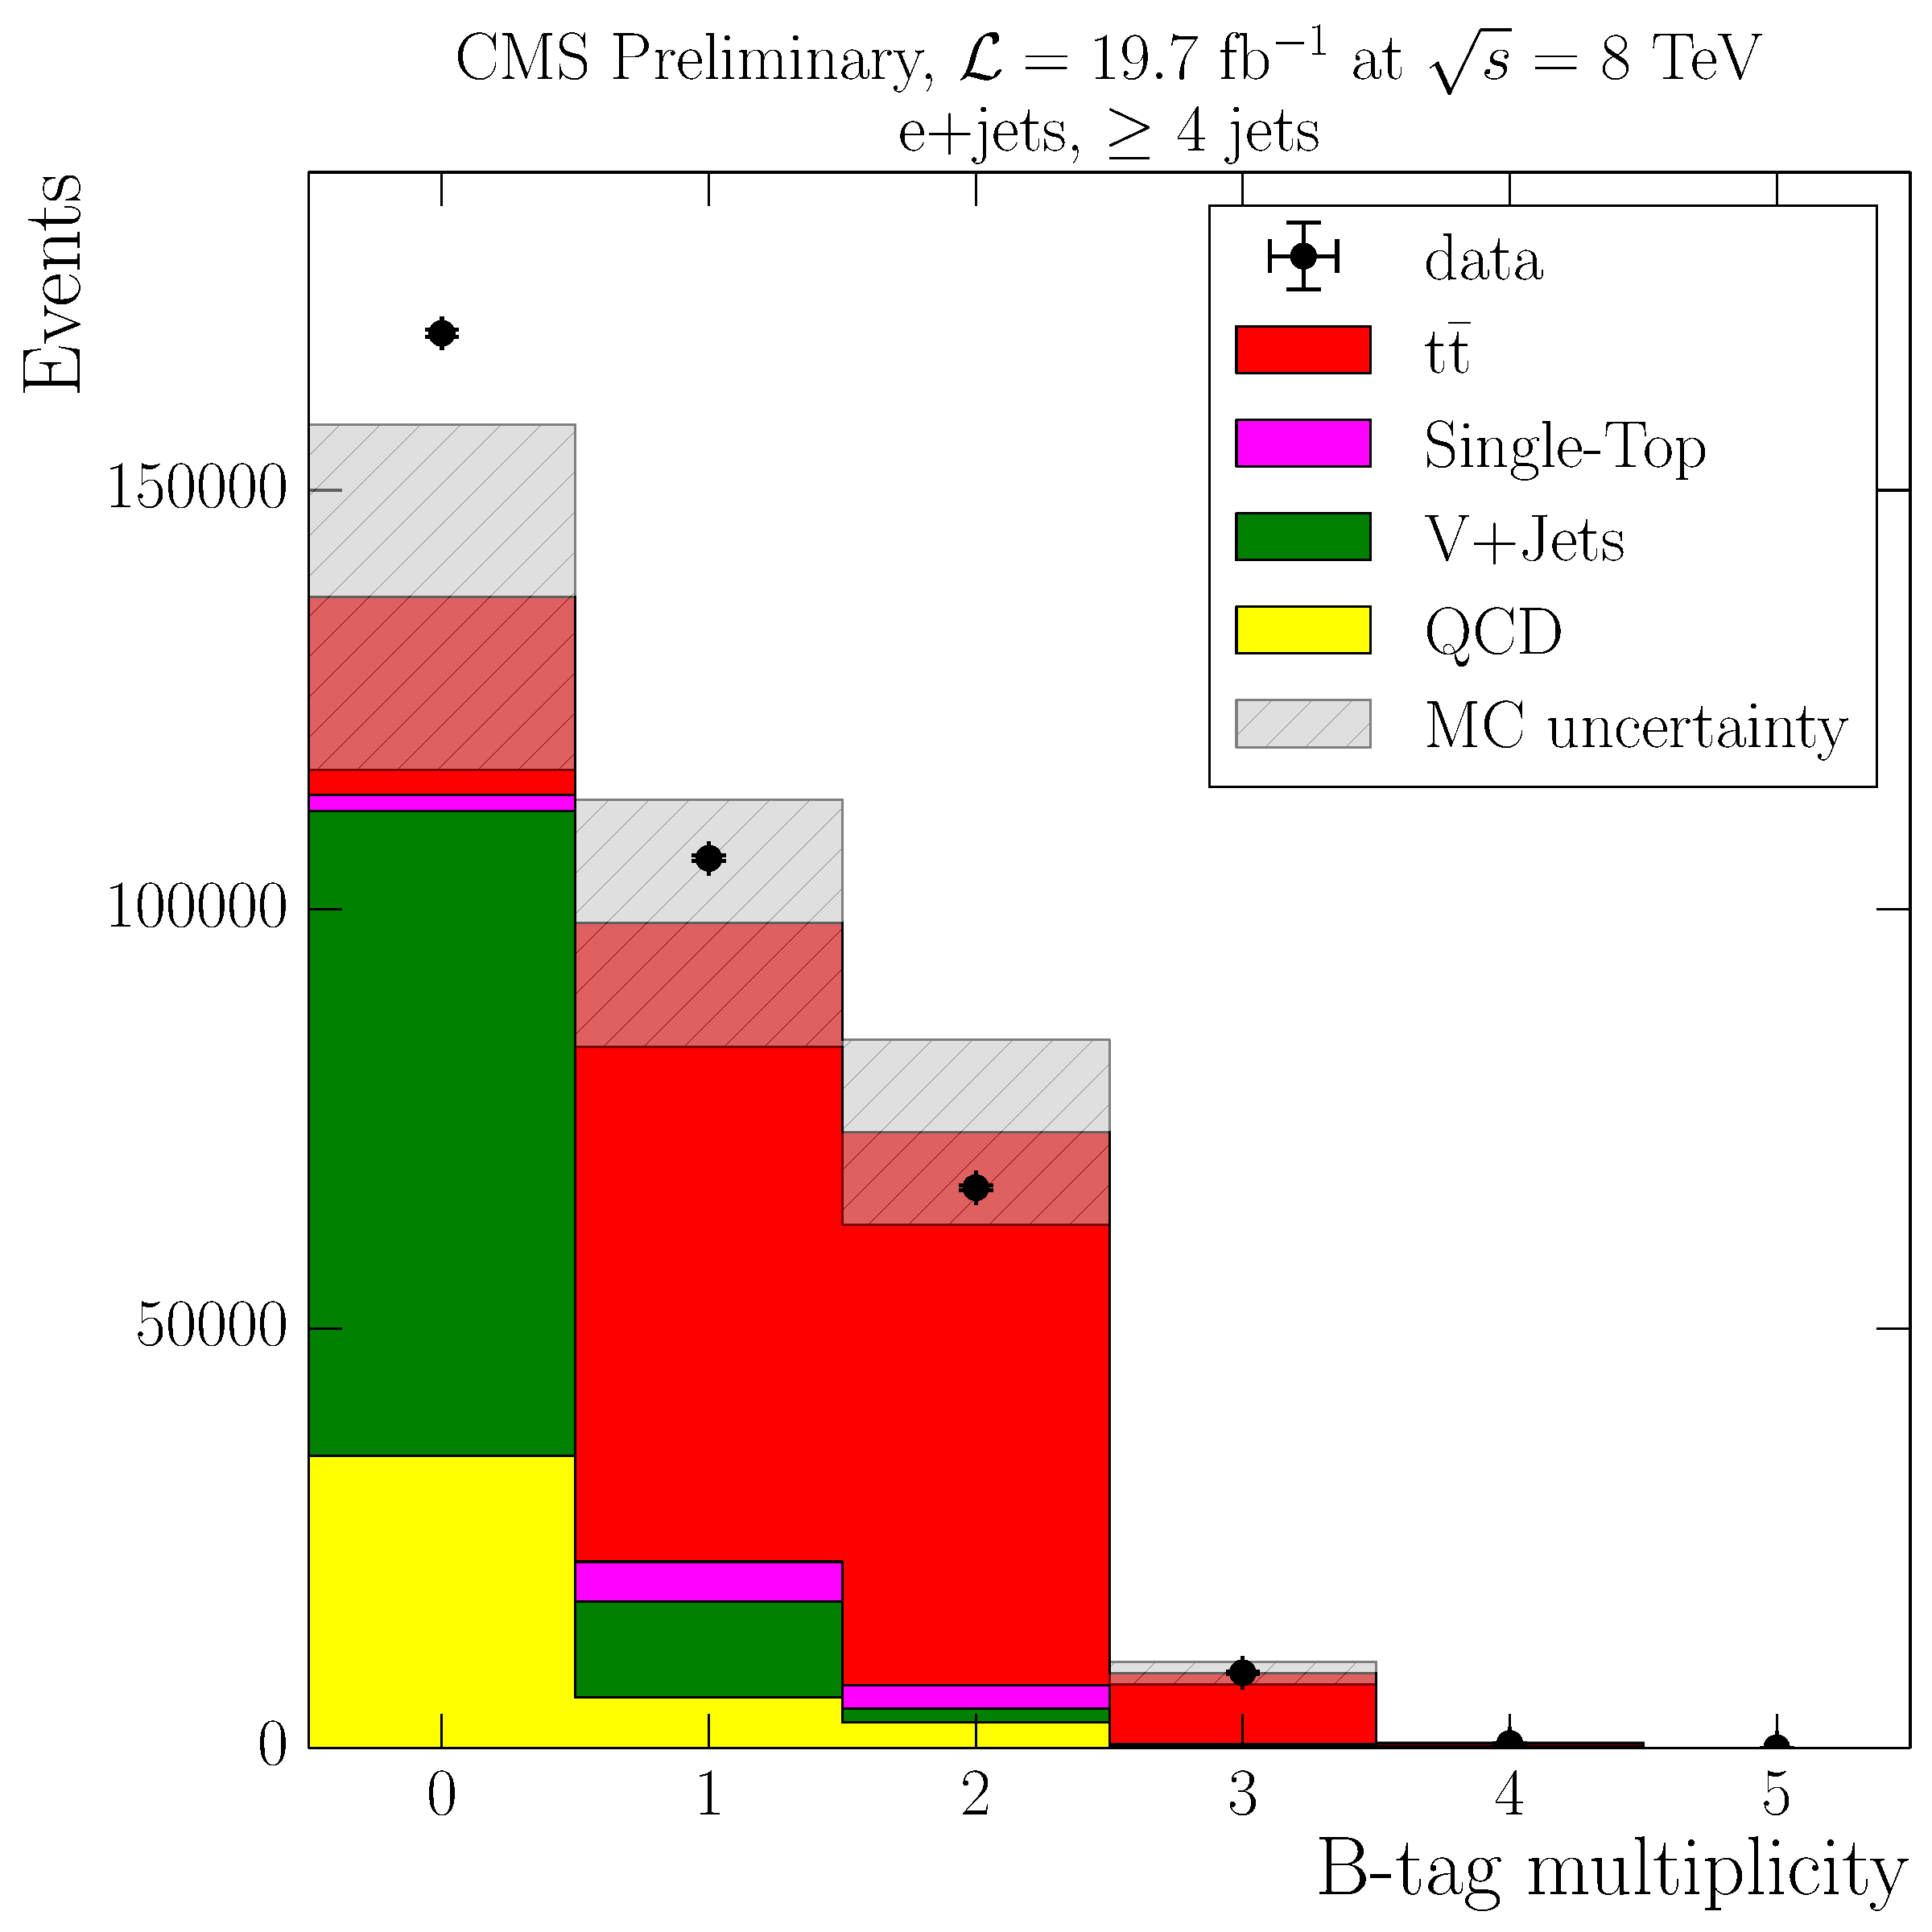
\includegraphics[width=0.50\textwidth]{bjets_multiplicity/EPlusJets_N_BJets.pdf}}\hfill
	\subfloat[]{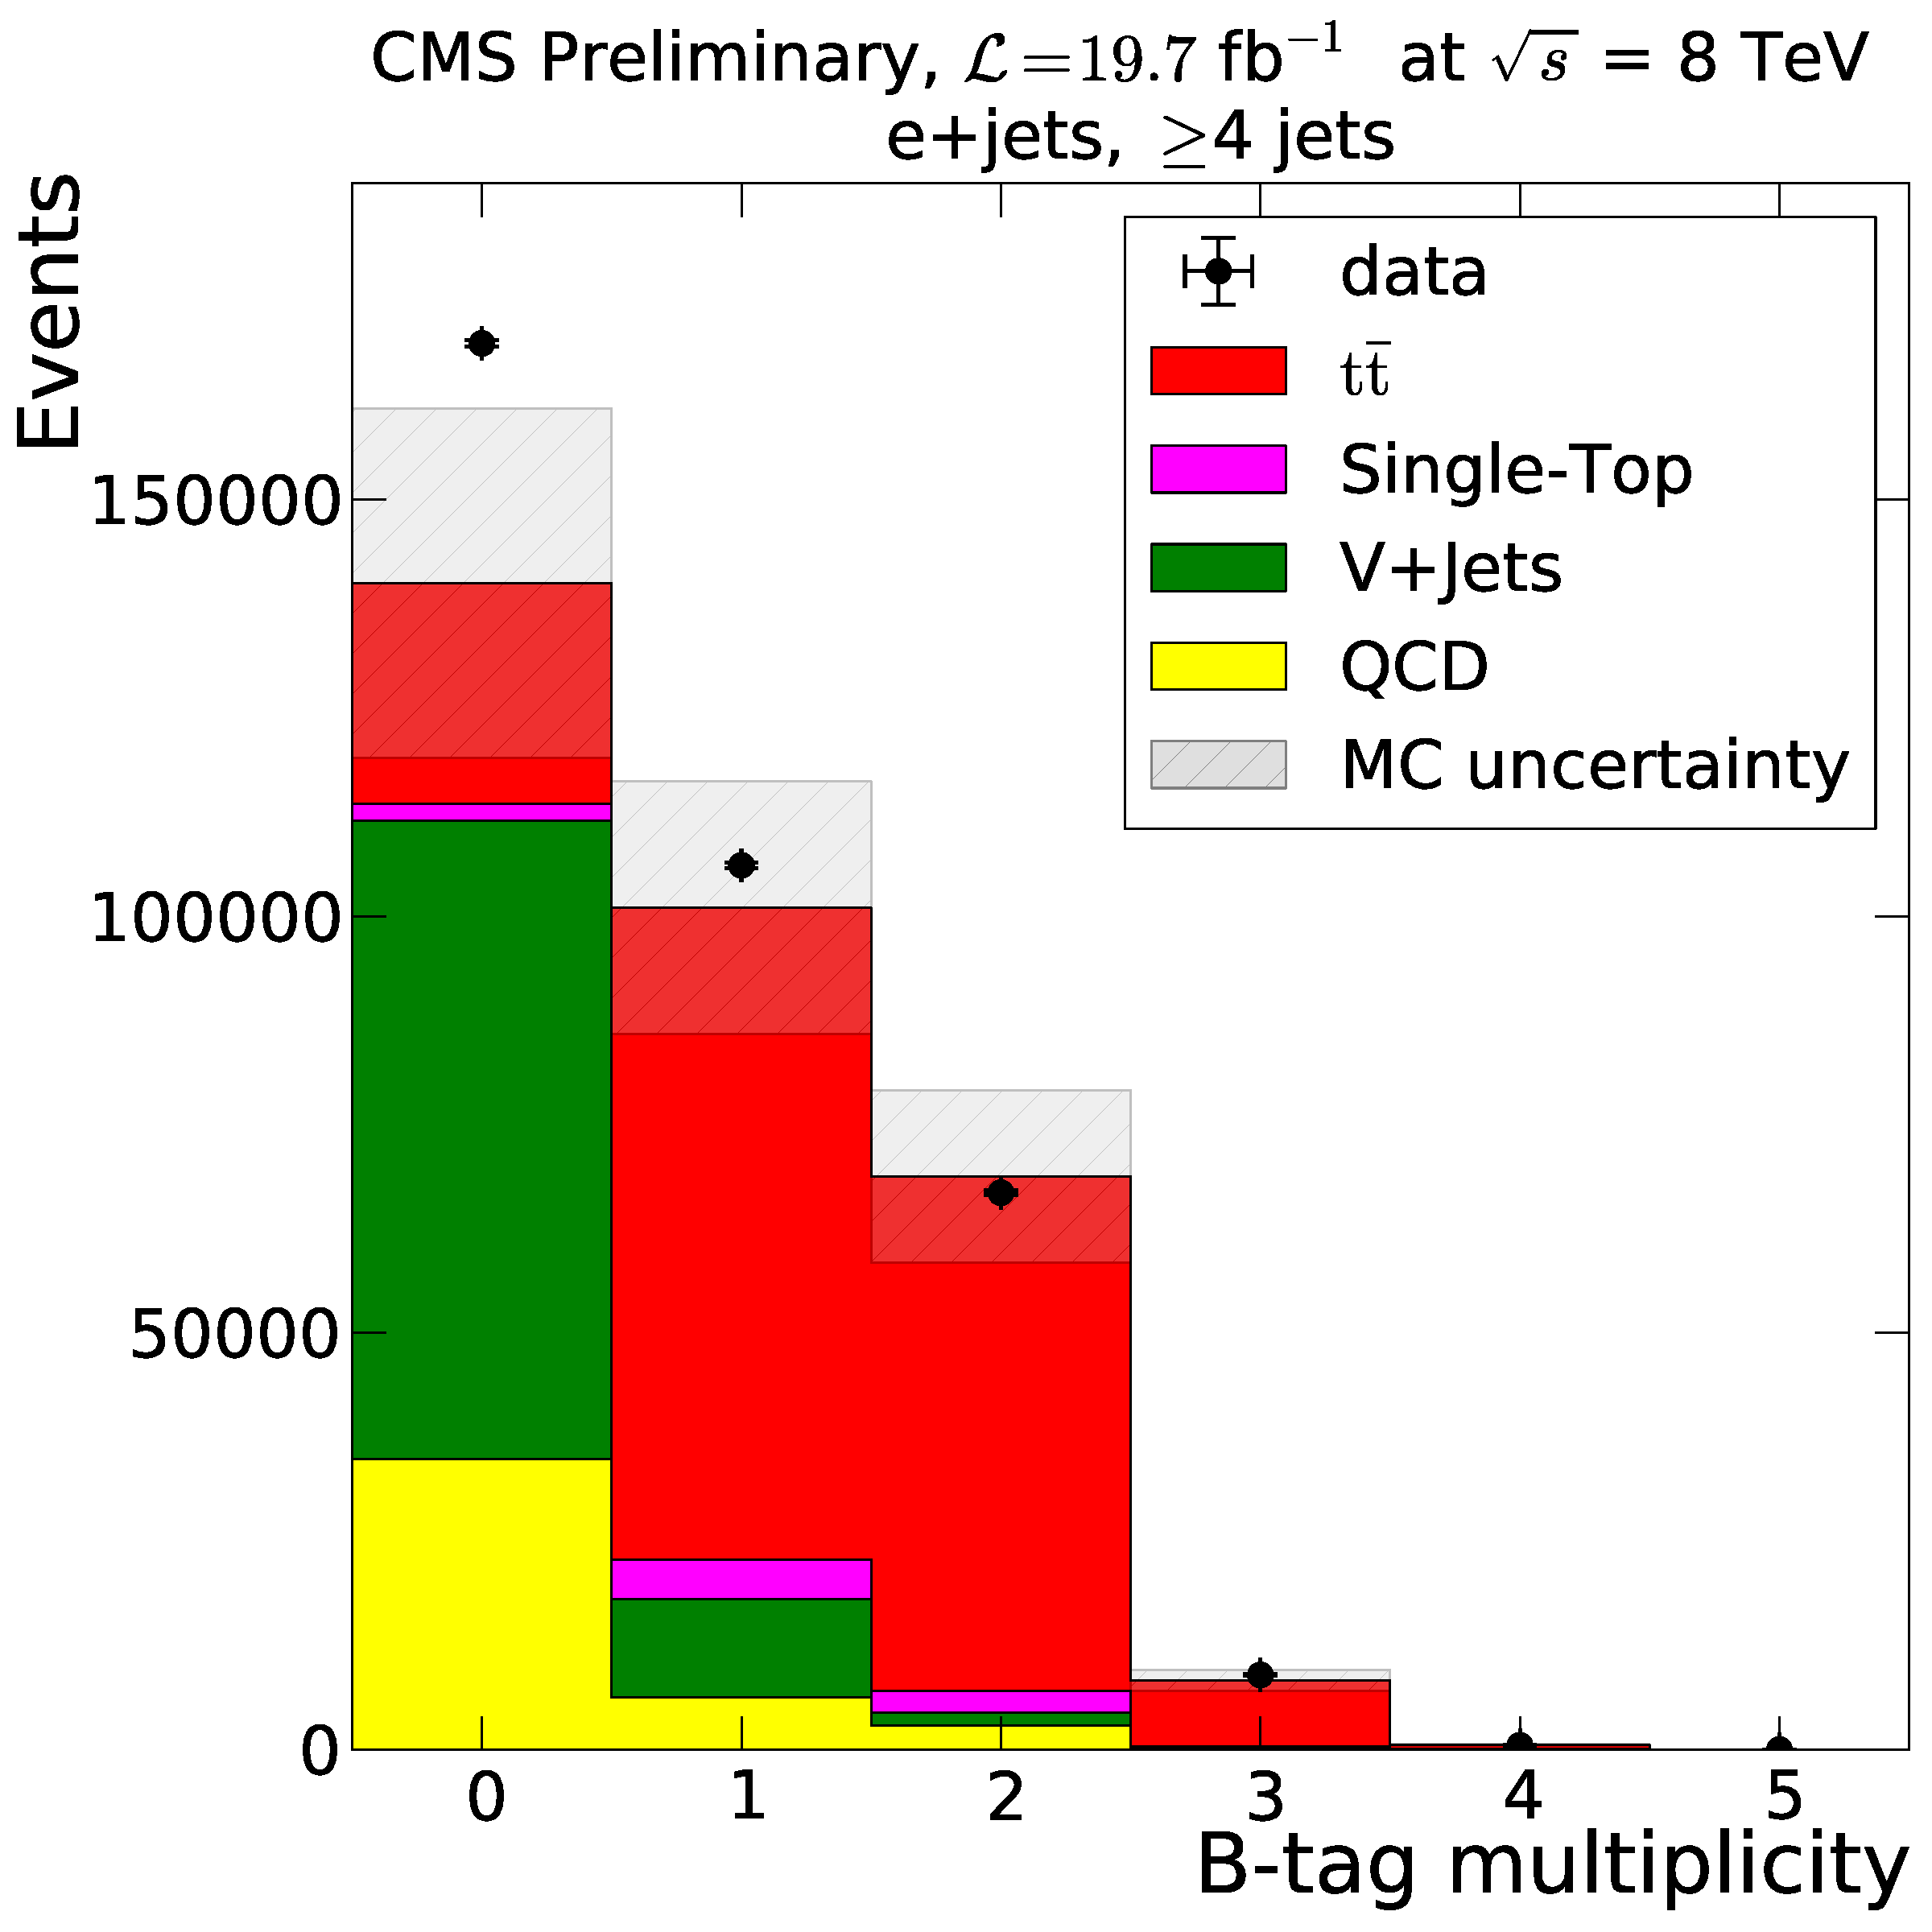
\includegraphics[width=0.50\textwidth]{bjets_multiplicity/EPlusJets_N_BJets_reweighted.pdf}} \\
	\subfloat[]{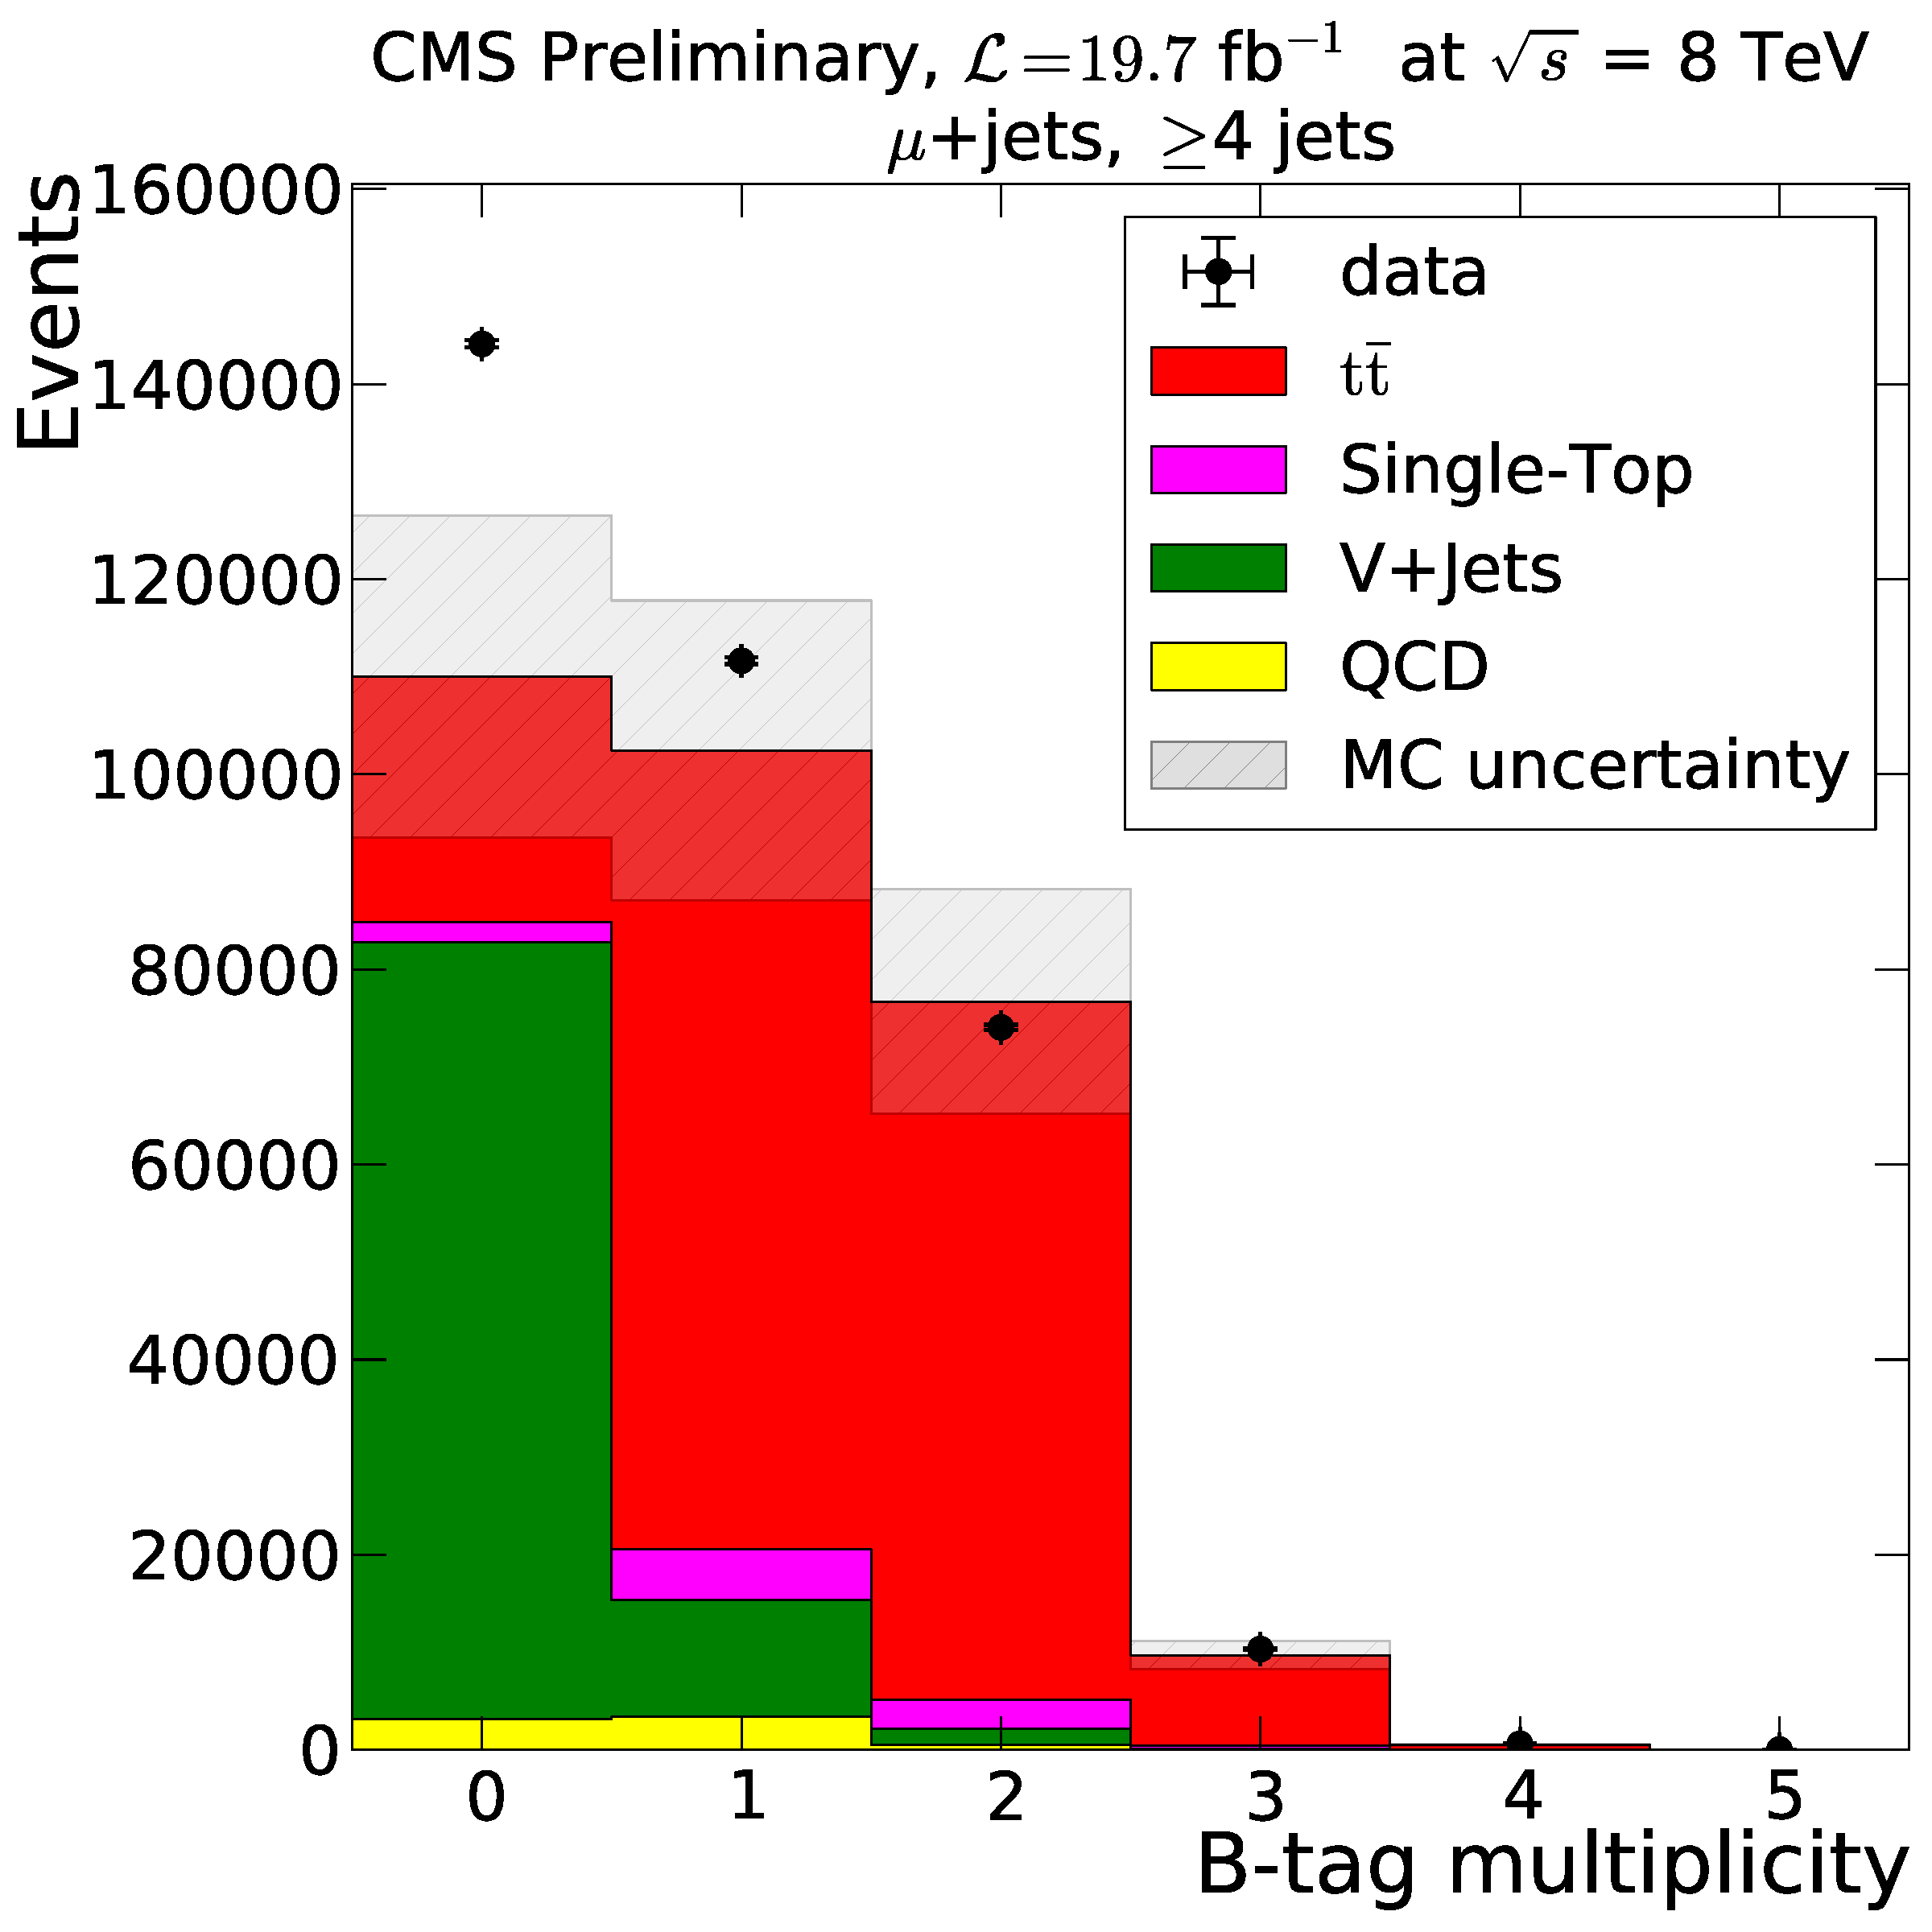
\includegraphics[width=0.50\textwidth]{bjets_multiplicity/MuPlusJets_N_BJets.pdf}}\hfill
	\subfloat[]{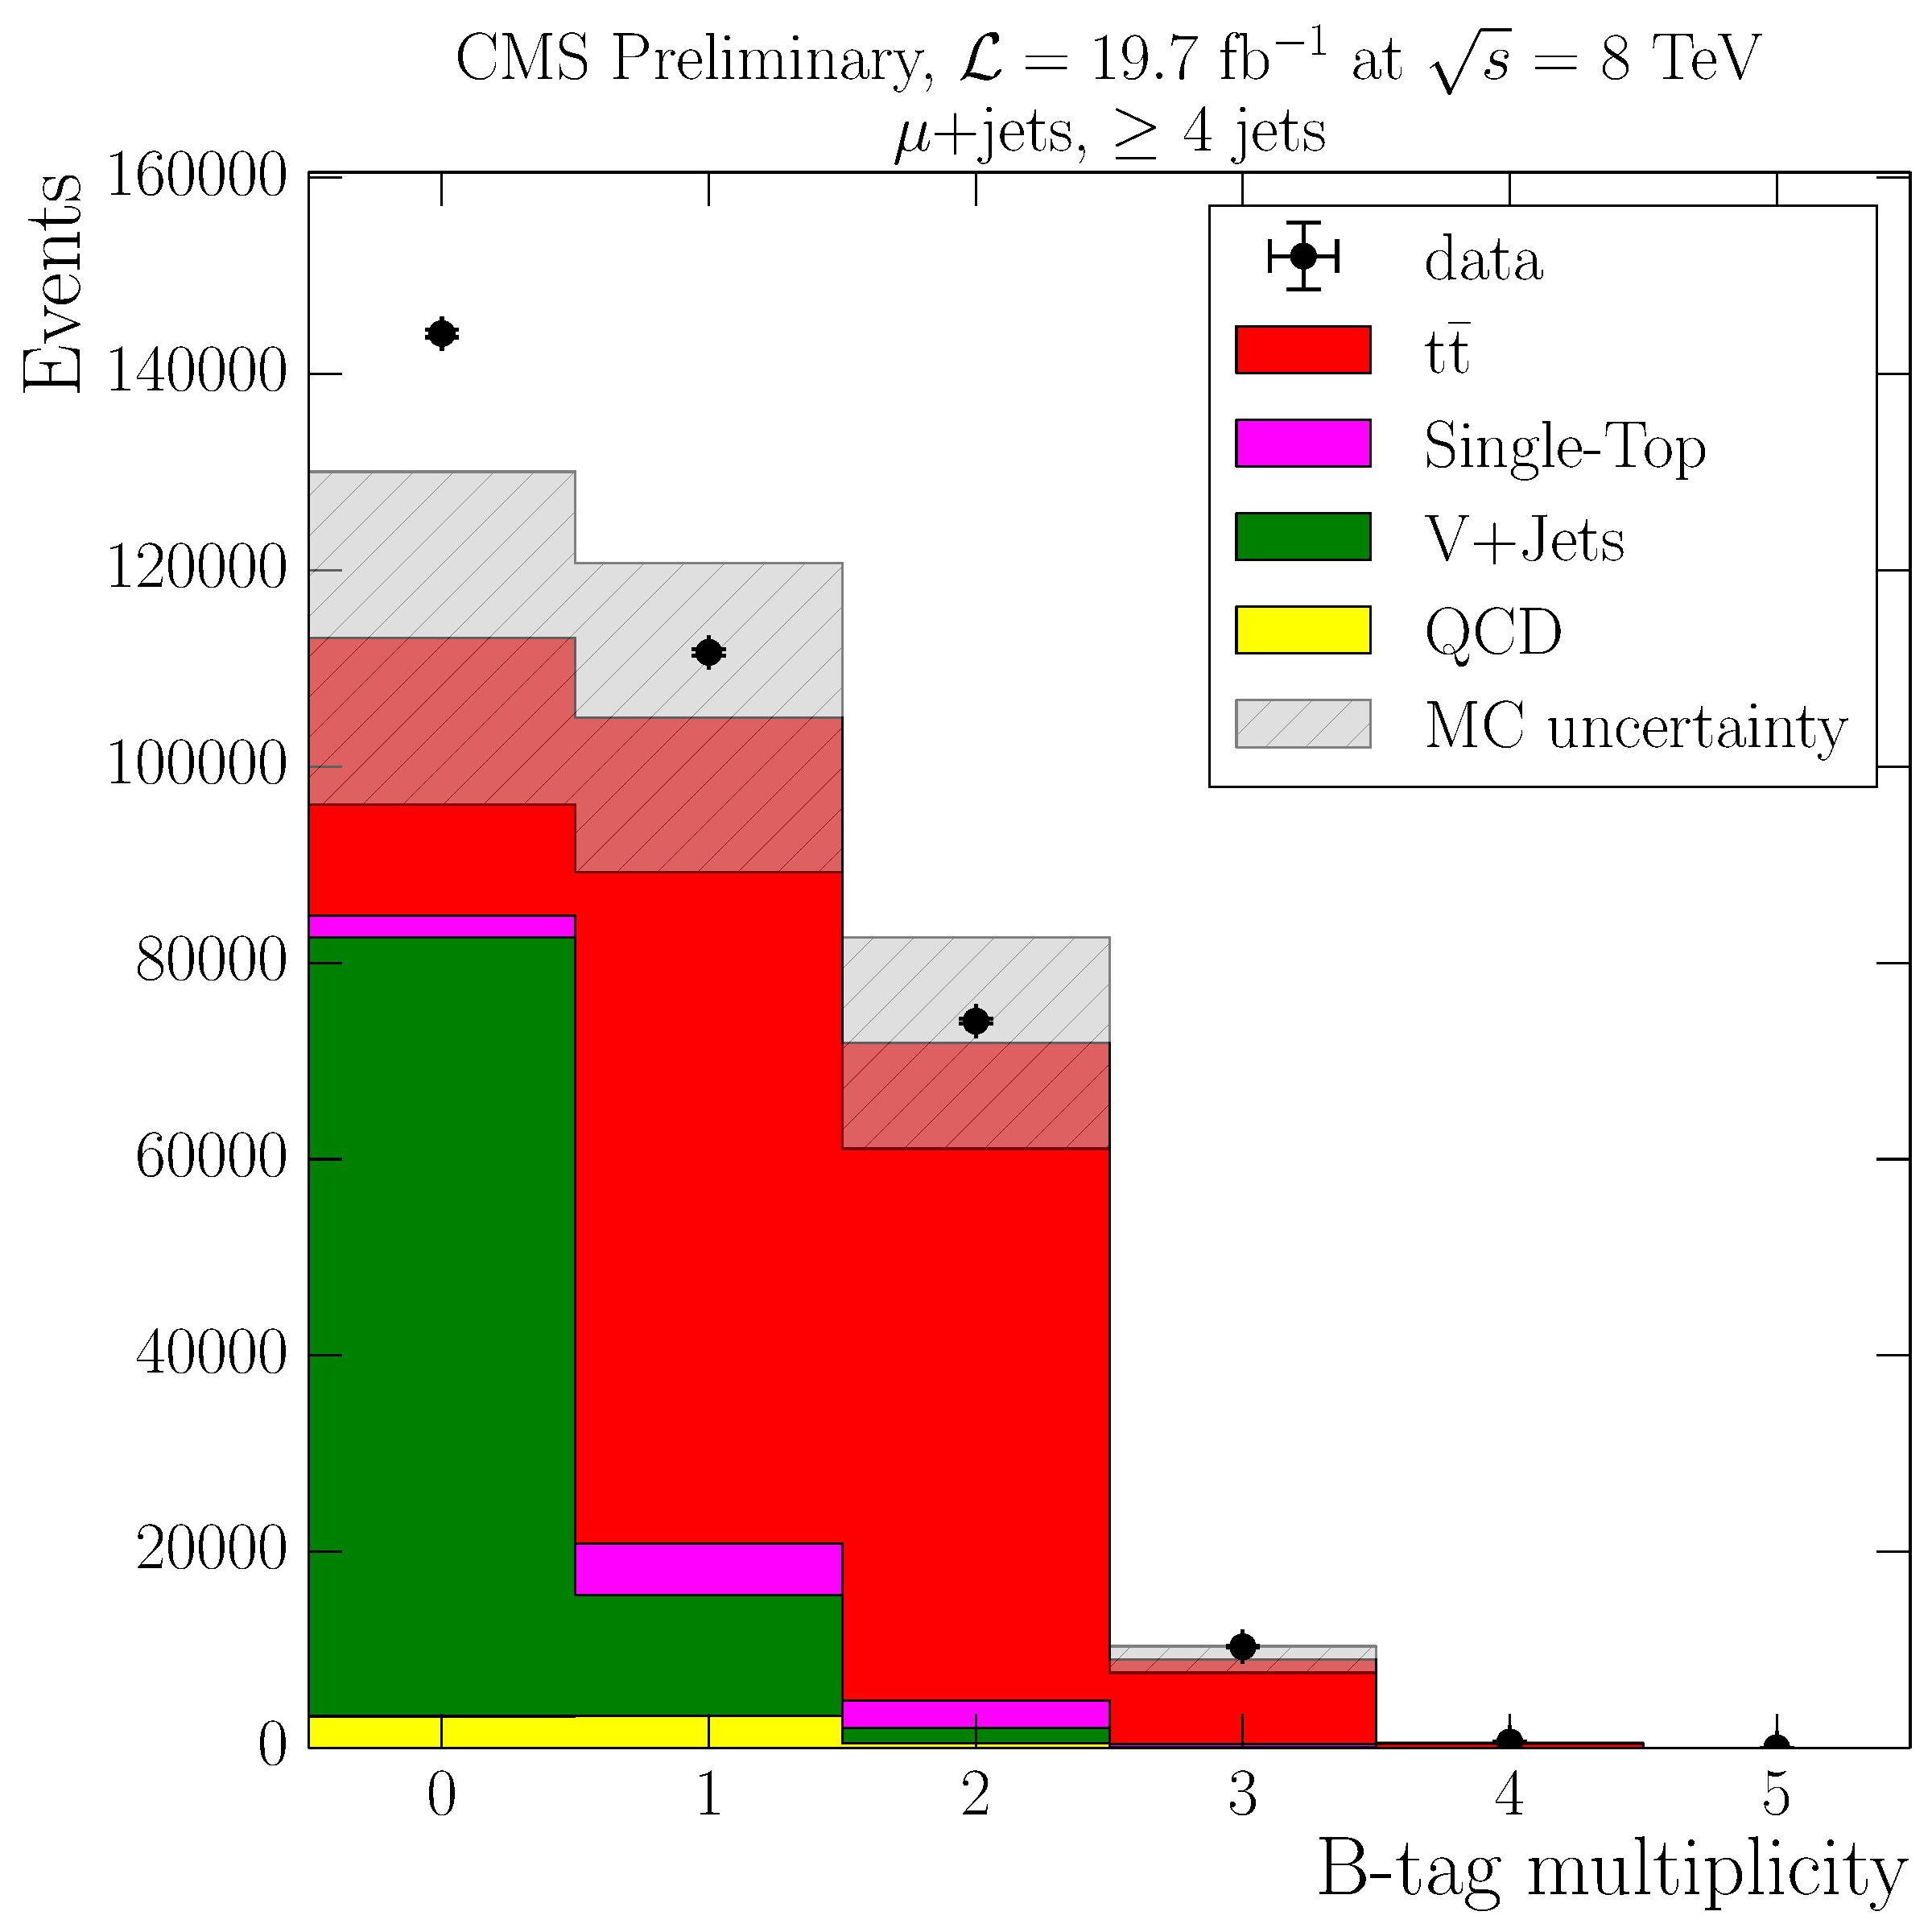
\includegraphics[width=0.50\textwidth]{bjets_multiplicity/MuPlusJets_N_BJets_reweighted.pdf}}
    \caption[b-tag multiplicity before and after applying the b-tagging scale factors]{b-tag multiplicity before (left)
    and after applying the b-tagging scale factors (right) in the electron channel (top) and the muon channel (bottom).}
    \label{fig:bjet_weights}
\end{figure}

Figure \ref{fig:bjet_weights} shows the results of the reweighting procedure for electron and muon channels. It can be
seen that the numbers of simulated events in b-tag multiplicity bins of \num{0} and \num{1} are scaled up, whereas for
other bins the number of MC events is scaled down. The systematic uncertainty due to b-tagging corrections is calculated
by applying $\pm 1 \sigma$ variations of the scale factors in the reweighting procedure.

\section{Event Selection}
\label{s_xsection:event_selection}
As in the top quark mass analysis, the event selection in this work is based on the standard CMS selection optimised for
Standard Model \ttbar production. It also exploits the semileptonic signature of a \ttbar decay with exactly one
isolated lepton and at least four jets, two of which are b-tagged. One of the main goals of the analysis is the
measurement of the missing transverse energy distribution represented by a neutrino from the leptonic decay of the \W
boson. Consequently, there is no specific requirement on the \MET in the selection.

Comparing to the 2011 event selection described in Section~\ref{s_top_mass:event_selection}, enhanced pile-up
subtraction and lepton identification techniques are used. Improved understanding of the detector in the form of updated
alignment and calibration constants resulted in better resolution of jets and \MET. The preselection (or skimming) step
used in order to reduce the number of events for local analysis processing is identical to that of the 2011 analysis.
However, additional filters are used to reject the events with artificial \MET caused by noise or known problems with
one of the detector subsystems. These filters are discussed in Section~\ref{ss_xsection:met_filters}.

Two semileptonic \ttbar decay modes are explored in this analysis: the electron plus jets and the muon plus jets
channels. The event selection for each of these decay modes is described hereafter.

\subsection{Electron plus jets channel}
\label{ss_xsection:ejets}

Similarly to the electron plus jets channel in the top quark mass analysis, the selection consists of the following
steps:

\begin{enumerate}[topsep=\parskip, parsep=\parskip, itemsep=\parskip, leftmargin=\leftmargin]
	\item preselection;
	\item trigger;
	\item electron candidate selection;
	\item muon veto;
	\item dilepton veto;
	\item conversion veto;
	\item jet selection;
	\item b-tagging.
\end{enumerate}

%https://twiki.cern.ch/twiki/bin/view/CMS/TWikiTop2011DataMCTrig

\subsubsection*{Trigger}
In contrast to the 2011 analysis using cross triggers, a single electron trigger is used in this analysis. Referred to
as HLT\_Ele27\_WP80, this trigger has a lepton \pt threshold of \SI{27}{\GeV} and ``WP80'' lepton isolation requirement
(see Table~\ref{tab:trigger_naming}), but no specific jet requirements. In 2012, the single electron trigger was
unprescaled for the whole running period, despite a comparatively large rate. The decision to keep the trigger
unprescaled was made due to simplicity of the trigger selection, requiring flat efficiency corrections.

\subsubsection*{Electron candidate selection}
Similarly to 2011 selection, exactly one electron candidate passing is required in the event, passing the following
criteria:

\begin{itemize}
	\item $\ET > \SI{30}{\GeV}$;
	\item $|\eta| < 2.5$, excluding the ECAL barrel-endcap transition regions of $1.4442 < |\eta| < 1.566$;
	\item MVA electron ID (Section~\ref{ss:electron_reconstruction}) with a discriminator cut of $>0.5$;
	\item transverse impact parameter with respect to the primary vertex $d_{xy} < \SI{0.02}{\cm}$;
	\item PF-based relative isolation (Section~\ref{sss:electron_isolation}) \reliso $< 0.1$ with a $\Delta
R$ cone of \num{0.3}.
\end{itemize}

\subsubsection*{Muon veto}
To reduce contamination from other \ttbar decay modes (i.e.\ muon and dilepton channels), events containing a global or
a tracker muon (see Section \ref{ss:muon_reconstruction}) are rejected. The requirements on the muon are identical to
those of 2011 selection: $\pt > \SI{10}{\GeV}$, $|\eta| < 2.5$ and $\reliso < 0.2$ with a $\Delta R$ cone of \num{0.4}.

\subsubsection*{Dilepton veto}
To reject events with additional electrons, a dilepton veto is applied. Events are rejected if they contain a second
electron candidate with the same ID and $\eta$ requirements, but looser \ET and \reliso criteria ($>\SI{20}{\GeV}$ and
$<0.15$, respectively).

\subsubsection*{Conversion veto}
As described in Section~\ref{sss:photon_conversions}, a vertex fit technique combined with the number of missing hits
in the tracker is used for photon conversion rejection.

\subsubsection*{Jet selection and b-tagging}
To help further reduce the background, at least four jets with $\pt > \SI{30}{\GeV}$ and $|\eta| < 2.5$ are required in
the event. These jets are required to pass the loose PF jet ID (see Section \ref{ss:jet_reconstruction}). Before the
multiplicity and identification requirements, the collection of jets is cleaned against the signal electron, i.e.\ any
jet within a $\Delta R$ cone of \num{0.3} around the signal lepton is excluded from the analysis. This is done due to
the fact that an electron may be reconstructed as a jet by leaving a characteristic signature in calorimeters. Any
additional jets with $\pt > \SI{20}{\GeV}$ and the same cleaning and ID requirements are also used for calculation of
\HT and \ST variables (Section~\ref{ss_xsection:variables}). Finally, the combined secondary vertex (CSV) b-tagging
algorithm with the medium working point (Section \ref{sss:b-tagging}) is used to identify the jets originating from
\cPqb-quarks in the \ttbar decay. At least two b-tagged jets are required in this analysis.

\subsection{Muon plus jets channel}
\label{ss_xsection:mujets}
The muon channel event selection follows a strategy similar to that of the electron channel:

\begin{enumerate}[topsep=\parskip, parsep=\parskip, itemsep=\parskip, leftmargin=\leftmargin]
	\item preselection;
	\item trigger;
	\item muon candidate selection;
	\item second muon veto;
	\item electron veto;
	\item jet selection;
	\item b-tagging.
\end{enumerate}

\subsubsection*{Trigger}
An isolated single muon trigger, referred to as HLT\_IsoMu24\_eta2p1, is used in this channel. Partially suggested by
the name of the trigger path, the following criteria on the muon are imposed at the HLT level:

\begin{itemize}
	\item $\pt > \SI{24}{\GeV}$;
	\item $\abs \eta < 2.1$;
	\item Combined tracker and calorimeter-based relative isolation (Section~\ref{sss:electron_isolation}) \reliso $<
0.15$ with a $\Delta R$ cone of 0.3.

% according to https://twiki.cern.ch/twiki/bin/viewauth/CMS/MuonHLT isolation used to be 0.1, dR=0.24 in RunA
\end{itemize}

\subsubsection*{Muon candidate selection}
For selection of a muon candidate, exactly one muon satisfying the following requirements is required:

\begin{itemize}
	\item $\pt > \SI{26}{\GeV}$;
	\item $|\eta| < 2.1$;
	\item PF-based relative isolation (Section~\ref{sss:electron_isolation}) \reliso $< 0.12$ with a $\Delta
R$ cone of \num{0.4};
	\item PF-muon ID criteria (Section \ref{ss:muon_reconstruction}):
	\begin{itemize}
		\item identified as a particle flow muon and as a global muon;
		\item a normalised $\chi^2$ of the global muon fit $<10$;
		\item number of muon chamber hits $>0$;
		\item number of muon stations with muon segments $>1$;
		\item transverse impact parameter w.r.t. the primary vertex $d_{xy} < \SI{0.02}{\cm}$;
		\item longitudinal distance of the tracker track w.r.t. the primary vertex $d_z < \SI{0.5}{\cm}$;
		\item number of hits in the pixel detector $>0$;
		\item number of hits in the tracker layers $>5$.
	\end{itemize}
\end{itemize}

\subsubsection*{Second muon veto}
Events containing an additional loose muon are rejected, with loose ID requirements as follows:

\begin{itemize}
	\item $\pt > \SI{10}{\GeV}$;
	\item $|\eta| < 2.5$;
	\item PF-based relative isolation (Section~\ref{sss:electron_isolation}) \reliso $< 0.2$ with a $\Delta R$ cone of
	\num{0.4}; %PU corrections!
	\item identified as a particle flow muon, and either global or tracker muon.
\end{itemize}

These criteria are identical to the muon veto requirements in the electron channel.

\subsubsection*{Electron veto}
To further reduce background contamination, events with electrons are rejected. The requirements on additional loose
electron are the same to the dilepton veto in the electron channel.

\subsubsection*{Jet selection and b-tagging}
Finally, the jet requirements are applied. These are also identical to those of the electron channel, mentioned above.


\subsection{Additional filters for missing transverse energy}
\label{ss_xsection:met_filters}
%https://twiki.cern.ch/twiki/bin/viewauth/CMS/MissingETOptionalFilters

There is no specific requirement on missing transverse energy in the selection, however, a set of corrections is applied
to \MET. As described in Section~\ref{ss:MET_reconstruction}, jet energy corrections are propagated to \MET, and it is
also corrected for pile-up and various detector effects causing $\phi$ modulation.

Additionally, a set of optional filters, prescribed for analyses with high sensitivity to \MET, was applied in the
selection for both electron and muon channels. Most of these filters were put in place after discovering events with
anomalously high missing transverse energy. A short description of each filter is given below.

\begin{description}[wide=\parindent]
	\item[CSC beam halo filter.]
	Protons in the LHC beams can interact with residual particles of beam collimators, which produces secondary particle
	showers referred to as beam halo \autocite{beam_halo_CMS}. This machine-induced background can significantly
	contaminate collision events, particularly affecting the \MET observable due to specific trajectories of halo muons.
	A dedicated algorithm based on exploiting the halo signatures in the Cathode Strip Chambers (CSCs) helps to mitigate
	this background.

	\item[HCAL laser filter.] The HCAL laser system is used for calibration and monitoring the detector response
	\autocite{CMS_TDR1}. During the 2012 data-taking, laser pulses were accidentally fired and consequently polluted a
	small fraction of the recorded physics dataset. Using the fact that unlike physics events, laser pulses produce hits
	in calibration channels of the HCAL, the dataset is filtered from this contamination.
	%https://indico.cern.ch/event/169318/contribution/1/material/slides/0.pdf

	\item[ECAL dead cell filter.] Both ECAL endcap and barrel regions are known to have faulty crystals producing too
	much noise in detector readouts. There are also crystals corresponding to front-end cards with defective data link.
	All these channels are masked in reconstruction and constitute to about \SI{1}{\pc} of the total amount. However,
	they can still cause a significant amount of energy deposits to be lost, therefore contributing to fake \MET. One of
	the approaches to tackle this issue uses the so-called trigger primitive information, i.e.\ digital quantities
	produced by the Level 1 trigger electronics \autocite{CMS_L1_Trigger_TDR}. Another approach uses the energy deposits
	surrounding the masked channels (boundary energy). These methods allow to filter events with the estimated energy
	leakage above certain threshold (\SI{\sim10}{\GeV}).
	%https://twiki.cern.ch/twiki/bin/viewauth/CMS/SusyEcalMaskedCellSummary

	\item[Tracking failure filter.] Some events have been observed to have a lack of tracks corresponding to standard or
	large calorimeter deposits. There are two understood sources of this misreconstruction: in a first type of such
	events, the tracking algorithm (explained in Section~\ref{ss:electron_reconstruction}) halts for some of its
	iterations due to an exceeding number of calorimeter clusters. In a second type the hard collision happens in a
	satellite colliding bunch at a distance of approximately \SI{75}{\cm} from the nominal interaction point along the
	$z$ axis. A cut on the summed \pt of the tracks originating from the primary vertices passing the preselection
	criteria, divided by the summed \pt of all jets in the event, was found to clearly distinguish between pathological
	and unaffected events. A cut value of \SI{10}{\pc} is imposed.
	%https://twiki.cern.ch/twiki/bin/viewauth/CMS/SusyRA2NJetsInData2010#Tracking_failure

	\item[Bad ECAL endcap super-cluster filter.] In 2012, two $5\times5$ super-clusters in the ECAL endcap regions were
	observed to occasionally produce anomalous pulses, leading to artificially high \MET. The source of this issue can
	be related to the High-Voltage system, but is subject to further investigation. A filter removing the problematic
	events is used, configured to cut on the total energy of reconstructed hits not passing the nominal quality criteria
	in the two super-clusters, with the cut value of \SI{1}{\TeV}.
	%https://twiki.cern.ch/twiki/bin/viewauth/CMS/MissingETOptionalFilters#Bad_EE_Supercrystal_filter_added

	\item[ECAL laser correction filter.] Lead tungstate crystals of the ECAL naturally lose their transparency with
	radiation exposure. To maintain high precision, this effect is corrected for by frequently injecting laser pulses
	and reading out the response in order to calibrate each crystal \autocite{CMS_TDR1}. During 2012 data-taking, a
	handful of crystals had unphysically large values of laser corrections, resulting in anomalously high \MET in
	recorded events. The filter removes such events from the dataset.
	%https://twiki.cern.ch/twiki/bin/viewauth/CMS/PdmVKnowFeatures#Filter_to_reject_events_with_ano

	\item[Strip tracker noise filter.] A few events were affected by a large coherent noise in the silicon strip
	tracker, which resulted in a much larger number of the strip clusters compared to according pixel cluster
	multiplicity in the tracking algorithm. A dedicated filter rejects events with this anomaly.
	%https://twiki.cern.ch/twiki/bin/viewauth/CMS/TrackingPOGFilters#Filters

\end{description}

Although the number of events removed by these filters is extremely small (\SI{\ll1}{\pc}), most of them have high fake
\MET, which could lead to an artificial excess in the \MET distribution. Due to the analysis sensitivity to \MET,
application of these filters was of high importance.

\section{Data-driven QCD Estimation}
\label{s_xsection:data_driven_QCD}
QCD multi-jet events constitute an important background to semileptonic \ttbar decays, and one of the most difficult to
model (Section~\ref{ss:backgrounds}). The requirement of two b-tagged jets in the event selection is mainly motivated by
the necessity to mitigate the effect of this particular background. In this analysis, the final QCD yield is obtained
from the fitting process as explained in Section~\ref{s_xsection:measurement}. However, the initial estimate is
performed using data-driven techniques. Only the shape of the distribution is of importance here as the normalisation is
determined in the fitting process. The QCD estimation methods for both electron and muon channel are described in detail
hereafter.

\subsection{QCD multi-jet events with electrons}
Two control regions have been investigated in the electron channel:

\begin{itemize}
\item conversion control region: conversion veto is inverted in the full event selection;
\item non-isolated electron control region: the electron isolation requirement is changed from $\reliso < 0.1$ to
$\reliso > 0.2$.
\end{itemize}

Additionally, only events with no b-tagged jets are taken into account to increase the statistics and QCD purity in both
control regions. In Figure~\ref{fig:qcd_control_regions_eta} the distributions of the absolute pseudorapidities of the
electron are presented for both control regions. The distributions observed in data are compared with MC expectations.
It can be seen that the distributions are not well described by the Monte Carlo, e.g.\ occasional high peaks in the QCD
MC represent the lack of statistics in simulation. Moreover, the two control regions have considerably different shapes
in the electron $\abs \eta$ distributions. For the conversion control region, the shape is mostly flat in the barrel
region ($\abs \eta < 1.5$) and peaks in the endcap region ($\abs \eta > 1.5$), which is expected as the conversions are
more likely to happen in the region with higher material budget. In contrast, the non-isolated control region peaks in
the pseudorapidity region of $1.0 < \abs \eta < 1.5$. Such behaviour is correlated with the jet $\abs
\eta$ distribution, since this control region favours non-isolated electrons coming from heavy quark decays.

\begin{figure}[htbp]
	\centering
  	\subfloat[]{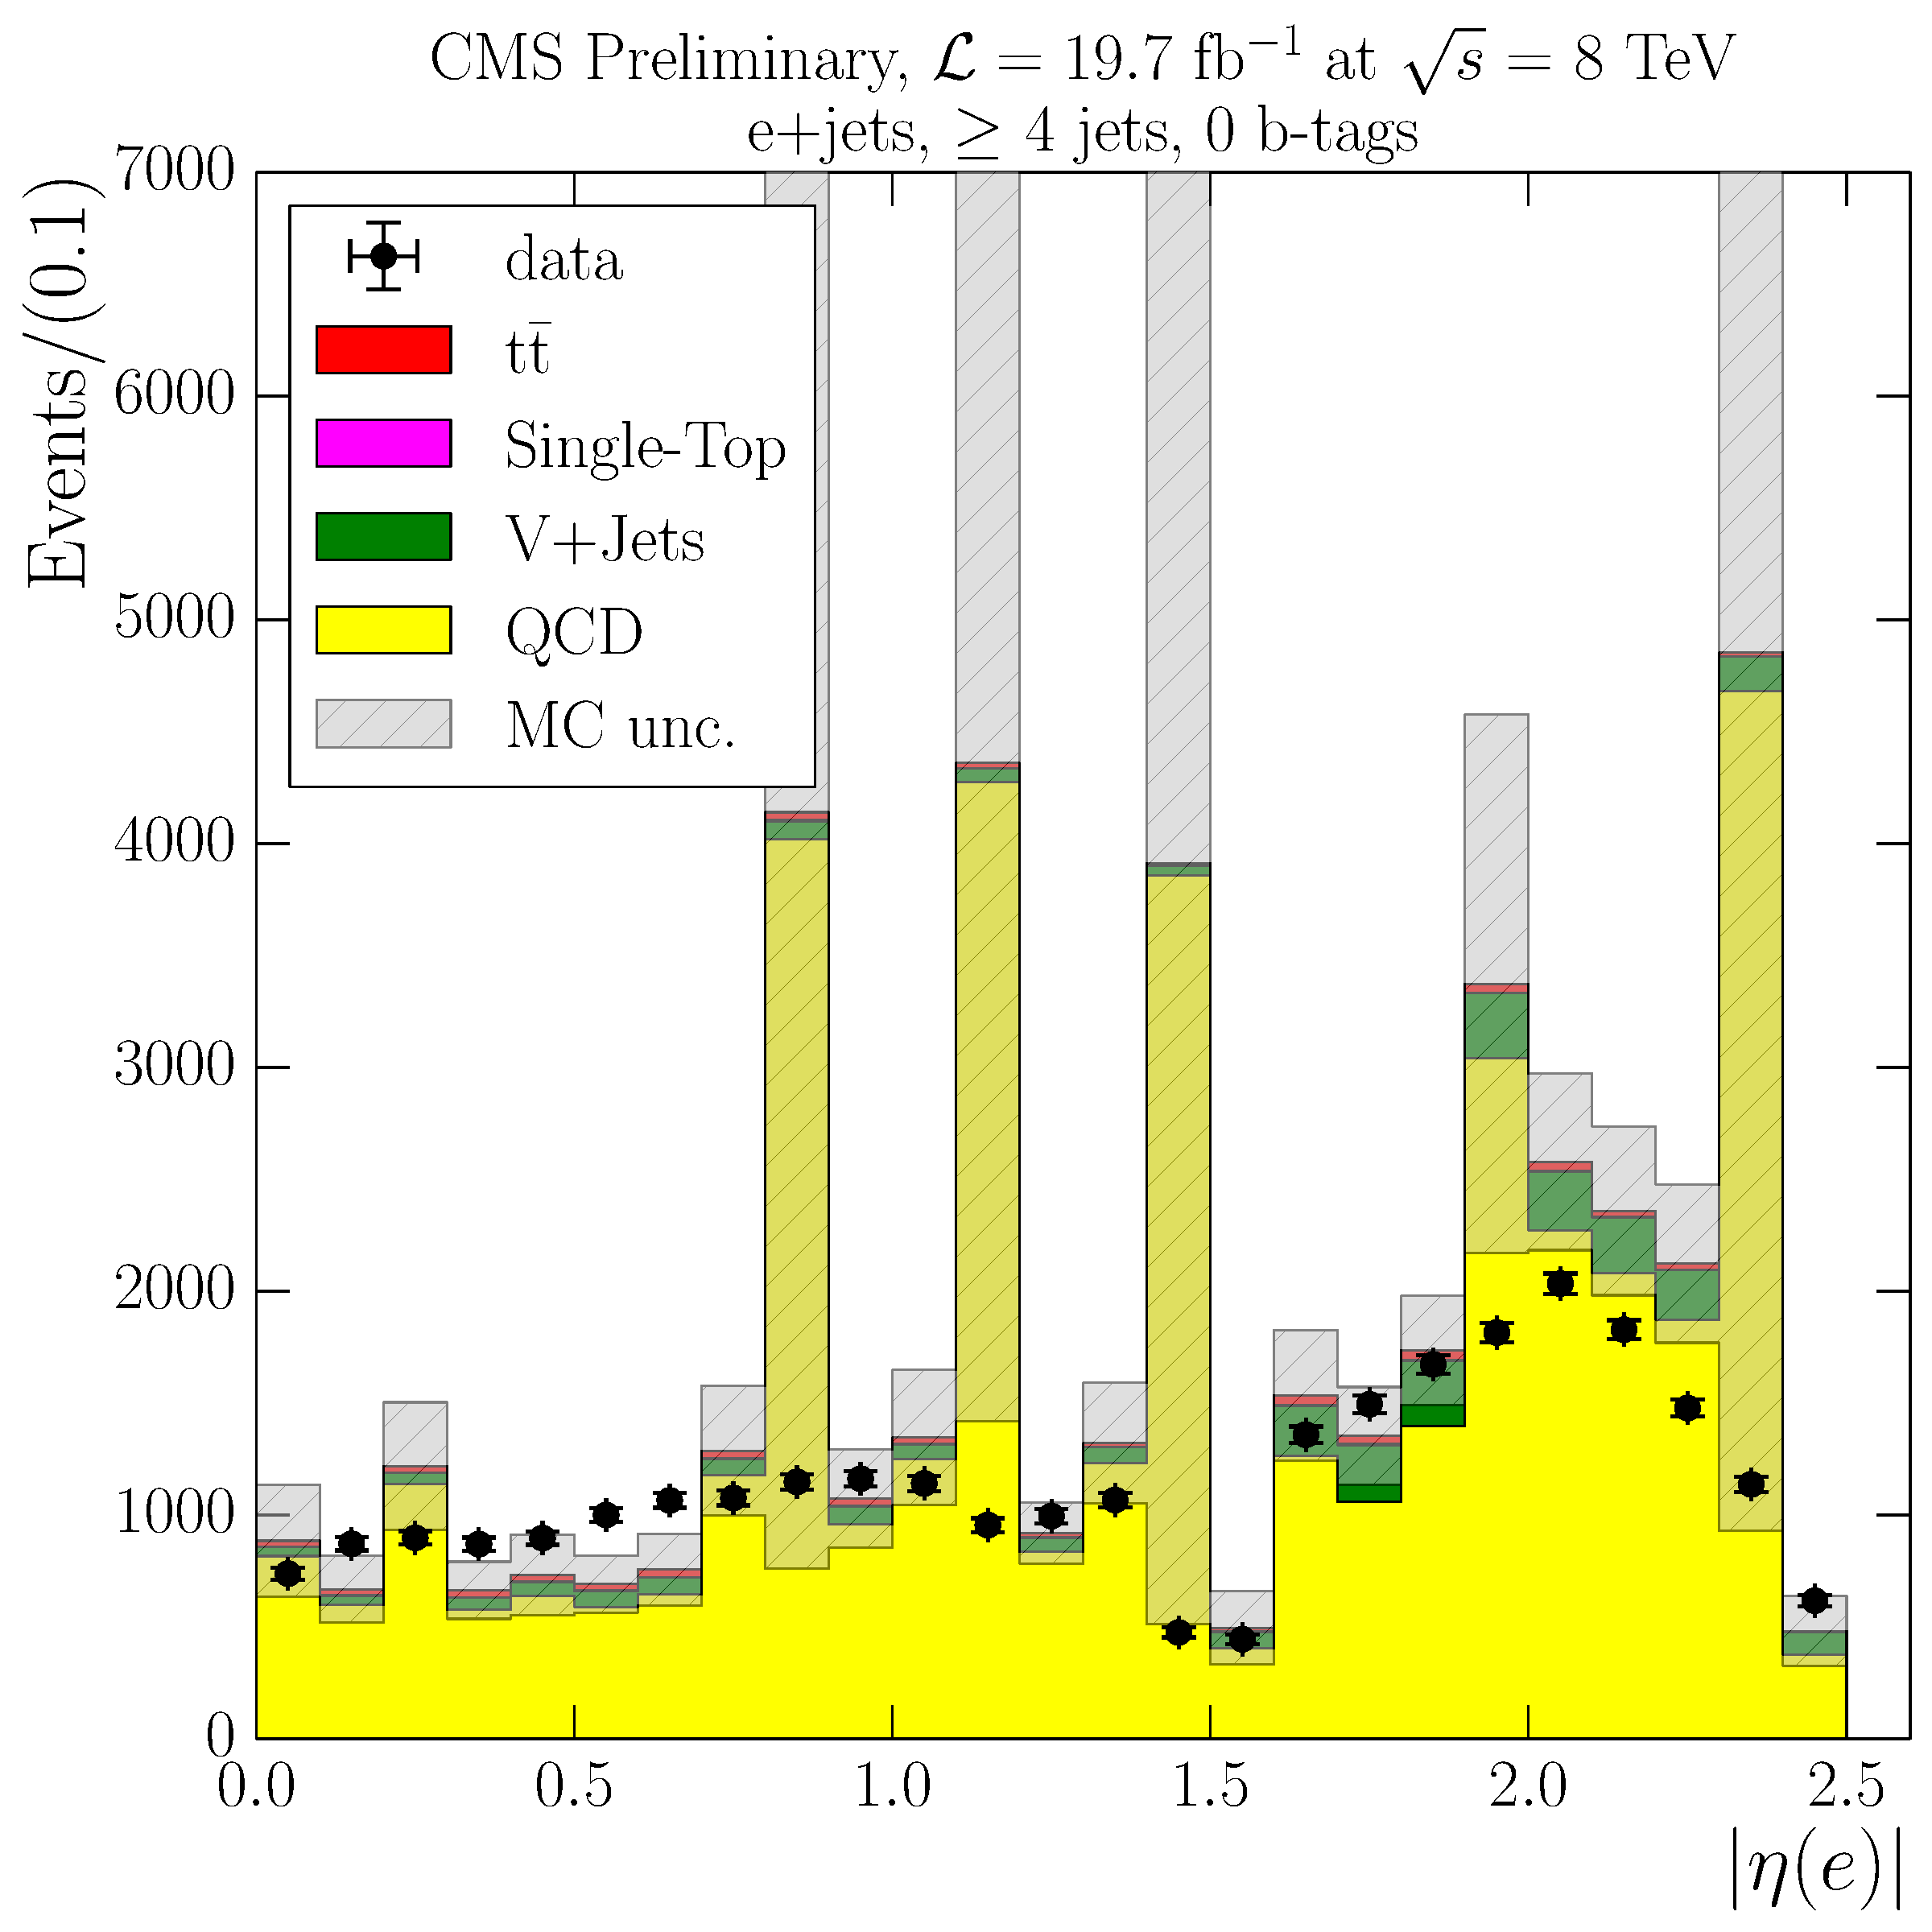
\includegraphics[width=0.50\textwidth]{QCD/QCD_conversion_control_region_electron_AbsEta_0btag}}\hfill
	\subfloat[]{\includegraphics[width=0.50\textwidth]{QCD/QCD_non_iso_control_region_electron_AbsEta_0btag}} \\
	\subfloat[]{\includegraphics[width=0.50\textwidth]{QCD/QCD_control_region_comparison_electron_AbsEta_0btag}}
    \caption[Distribution of the electron $\abs \eta$ for conversion selection and non-isolated electron selection, and
    the shape comparison of both QCD control regions]{Distribution of the electron $\abs \eta$ for conversion selection
    (a), non-isolated electron selection (b) and the shape comparison of both QCD control regions in data (c) in
    electron plus jets events with at least four jets and 0 b-tagged jets.}
    \label{fig:qcd_control_regions_eta}
\end{figure}

Also, in Figure~\ref{fig:qcd_control_regions_eta} we see that while the conversion region is predicted to be a rather
pure QCD sample, the non-isolated control region has significant contamination from \ttbar signal and \W/\ZpJets events.
For this reason, the conversion region was chosen to produce the QCD template for the electron channel. However, since
the relative contributions of the QCD events from both control regions in the final selected sample are not known, the
real QCD shape can differ considerably from the prediction. Therefore, the non-isolated region is used to estimate the
systematic uncertainty due to the QCD shape choice. This systematic error is estimated by substituting the nominal QCD
template from the conversion control region with that from the non-isolated region, and calculating the change in the
final measurement. More information on systematic uncertainties is presented in Section~\ref{s_xsection:systematics}.

\subsection{QCD multi-jet events with muons}
For the QCD shape extraction in the muon plus jets channel, the inverted isolation cut is applied in the event
selection: at least one muon with $\reliso>0.3$ is required, and events with isolated muons with $\reliso<0.3$ are
vetoed. Similarly to the electron channel, only events with no b-tagged jets are taken into account. Additionally, to
increase the available statistics, events with only three jets are also considered. %($\geq 3$ jet bin).

The relative isolation distribution with the cut value and the muon $\abs \eta$ for the non-isolated region are shown on
Figure~\ref{fig:qcd_muon_plots}. Clearly, the control region is dominated by QCD events and generally there is a
reasonable agreement between data and simulation. The contamination from other processes is subtracted using MC.

\begin{figure}[!htbp]
	\centering
	\vspace*{-0.35cm}
  	\subfloat[]{\includegraphics[width=0.47\textwidth]{QCD/QCD_muon_pfIsolation_0btag}}\hfill
  	\subfloat[]{\includegraphics[width=0.47\textwidth]{QCD/QCD_non_iso_control_region_muon_AbsEta_0btag}}
    \caption[Muon relative isolation with no isolation cut and muon $\abs \eta$ for non-isolated selection in muon plus
    jets events]{Muon relative isolation with no isolation cut (a) and muon $\abs \eta$ (b) for non-isolated ($\reliso >
    0.3$) selection in muon plus jets events with at least three jets and 0 b-tagged jets. The red line on plot (a)
    shows the \reliso cut value of \num{0.3}.}
    \label{fig:qcd_muon_plots}
\end{figure}

\section{Data/MC Comparison}
\label{s_xsection:data_mc_comparison}

In this section, the agreement between simulation and data for various kinematic distributions is reviewed after the
final event selection. The event yields for all selection steps described in Section~\ref{s_xsection:event_selection}
are shown in Tables~\ref{tab:event_yields_ejets} and \ref{tab:event_yields_mujets} for the electron and muon channels,
respectively. All background events are normalised to the number of expected events for the total integrated luminosity
of \SI{19.7}{\fbinv}.

The QCD multi-jet background events shown in plots are derived using the data-driven methods explained previously.
Figure~\ref{fig:contol_plots_leptons} shows the lepton \pt and $\abs \eta$ distributions for both electrons and muons.
In Figure~\ref{fig:contol_plots_METs}, missing transverse energy distributions are shown, also including the
logarithmic scale for higher values of \MET. Figure~\ref{fig:contol_plots_phiMET_NJets} shows the azimuthal angle of
\MET ($\phi(\MET)$) and jet multiplicity distributions for both channels. The \ttbar uncertainty shown in the plots
refers to the theoretical uncertainty on the NNLO calculation of the total \ttbar cross section at \SI{8}{\TeV}
\autocite{NNLO_ttbar} used in this analysis.

Overall, good agreement is found between data and Monte Carlo simulation in all kinematic distributions. One should note
that the comparison shown is made before the fitting process, which is described in
Section~\ref{s_xsection:measurement}.

\begin{table}
  \centering
   \caption[Number of expected and observed events from simulation and data in the electron channel]{Number of expected
   and observed events from simulation and data in the electron channel out of the box, i.e.\ before the fitting
   process.}
    \label{tab:event_yields_ejets}
    \resizebox{\columnwidth}{!} {
    \begin{tabular}{lrrrrrrr}
    \toprule
	\textbf{Selection step} & \textbf{\ttjets} & \textbf{\WpJets} & \textbf{\ZpJets} & \textbf{Single top} & \textbf{QCD} & \textbf{Sum MC} & \textbf{Data} \\
	\midrule
	Preselection  &  $1346476 \pm 1028$ &  $1727900 \pm 1138$ &  $380944 \pm 234$ &  $169689 \pm 262$ &  $130308513 \pm 475118$ &  $133933524 \pm 475120$ &  13042702 \\ 
	Event cleaning/HLT  &  $385009 \pm 553$ &  $516544 \pm 600$ &  $147515 \pm 143$ &  $37308 \pm 127$ &  $3854386 \pm 83441$ &  $4940764 \pm 83445$ &  5846672 \\ 
	One isolated electron  &  $342394 \pm 522$ &  $446691 \pm 548$ &  $100243 \pm 117$ &  $33000 \pm 120$ &  $578895 \pm 29802$ &  $1501225 \pm 29812$ &  1688811 \\ 
	Muon veto  &  $323759 \pm 508$ &  $446579 \pm 548$ &  $99805 \pm 117$ &  $32301 \pm 118$ &  $578860 \pm 29802$ &  $1481306 \pm 29812$ &  1668851 \\ 
	Dilepton veto  &  $319019 \pm 504$ &  $446469 \pm 548$ &  $73876 \pm 101$ &  $32117 \pm 118$ &  $578821 \pm 29802$ &  $1450305 \pm 29812$ &  1628009 \\ 
	Conversion veto  &  $310863 \pm 498$ &  $430191 \pm 538$ &  $70929 \pm 99$ &  $31287 \pm 116$ &  $321292 \pm 21826$ &  $1164563 \pm 21839$ &  1396638 \\ 
	$\geq 1$ jets  &  $310863 \pm 498$ &  $430179 \pm 538$ &  $70928 \pm 99$ &  $31287 \pm 116$ &  $321292 \pm 21826$ &  $1164550 \pm 21839$ &  1396638 \\ 
	$\geq 2$ jets  &  $310838 \pm 498$ &  $429195 \pm 536$ &  $70723 \pm 99$ &  $31279 \pm 116$ &  $320506 \pm 21819$ &  $1162543 \pm 21831$ &  1396506 \\ 
	$\geq 3$ jets  &  $306406 \pm 494$ &  $386892 \pm 493$ &  $63653 \pm 90$ &  $29953 \pm 114$ &  $226938 \pm 16321$ &  $1013843 \pm 16337$ &  1215535 \\ 
	$\geq 4$ jets  &  $174701 \pm 373$ &  $76646 \pm 179$ &  $13323 \pm 35$ &  $9765 \pm 67$ &  $44203 \pm 4340$ &  $318640 \pm 4361$ &  351194 \\ 
	$\geq 1$ b-tagged jets  &  $148287 \pm 341$ &  $11280 \pm 69$ &  $2152 \pm 14$ &  $7675 \pm 58$ &  $9304 \pm 2055$ &  $178700 \pm 2085$ &  182481 \\ 
	$\geq 2$ b-tagged jets  &  $70103 \pm 228$ &  $1320 \pm 23$ &  $337 \pm 5$ &  $2900 \pm 35$ &  $3035 \pm 1789$ &  $77697 \pm 1804$ &  76379 \\ 
	\bottomrule
	\end{tabular}
	}
\end{table}

\begin{table}
  \centering
   \caption[Number of expected and observed events from simulation and data in the muon channel]{Number of expected and
   observed events from simulation and data in the muon channel out of the box, i.e.\ before the fitting process.}
    \label{tab:event_yields_mujets}
    \resizebox{\columnwidth}{!} {
    \begin{tabular}{lrrrrrrr}
    \toprule
	\textbf{Selection step} & \textbf{\ttjets} & \textbf{\WpJets} & \textbf{\ZpJets} & \textbf{Single top} & \textbf{QCD} & \textbf{Sum MC} & \textbf{Data} \\
	\midrule
	Preselection  &  $1346476 \pm 1028$ &  $1727900 \pm 1138$ &  $380944 \pm 234$ &  $169689 \pm 262$ &  $104079124 \pm 236784$ &  $107704135 \pm 236789$ &  20284215 \\ 
	Event cleaning/HLT  &  $443056 \pm 581$ &  $644505 \pm 688$ &  $148143 \pm 142$ &  $44727 \pm 135$ &  $1664036 \pm 33747$ &  $2944468 \pm 33759$ &  3063569 \\ 
	One isolated muon  &  $360897 \pm 521$ &  $473825 \pm 556$ &  $88283 \pm 106$ &  $35546 \pm 121$ &  $83535 \pm 5833$ &  $1042088 \pm 5885$ &  1327738 \\ 
	Second muon veto  &  $353646 \pm 516$ &  $473776 \pm 556$ &  $53263 \pm 82$ &  $35260 \pm 120$ &  $82863 \pm 5823$ &  $998811 \pm 5874$ &  1254896 \\ 
	Electron veto  &  $336474 \pm 503$ &  $473631 \pm 556$ &  $52935 \pm 82$ &  $34633 \pm 119$ &  $82841 \pm 5823$ &  $980516 \pm 5873$ &  1237495 \\ 
	$\geq 1$ jets  &  $336474 \pm 503$ &  $473622 \pm 556$ &  $52934 \pm 82$ &  $34633 \pm 119$ &  $82841 \pm 5823$ &  $980507 \pm 5873$ &  1237495 \\ 
	$\geq 2$ jets  &  $336457 \pm 503$ &  $472377 \pm 554$ &  $52768 \pm 81$ &  $34620 \pm 119$ &  $81211 \pm 5777$ &  $977436 \pm 5827$ &  1237428 \\ 
	$\geq 3$ jets  &  $332863 \pm 501$ &  $425334 \pm 507$ &  $47493 \pm 74$ &  $33146 \pm 117$ &  $33505 \pm 2726$ &  $872343 \pm 2822$ &  1108272 \\ 
	$\geq 4$ jets  &  $188466 \pm 377$ &  $83248 \pm 184$ &  $10144 \pm 29$ &  $10556 \pm 67$ &  $7006 \pm 1155$ &  $299422 \pm 1231$ &  340786 \\ 
	$\geq 1$ b-tagged jets  &  $160223 \pm 344$ &  $12341 \pm 71$ &  $1690 \pm 12$ &  $8322 \pm 59$ &  $3763 \pm 910$ &  $186341 \pm 977$ &  196667 \\ 
	$\geq 2$ b-tagged jets  &  $76068 \pm 231$ &  $1465 \pm 24$ &  $248 \pm 4$ &  $3096 \pm 35$ &  $481 \pm 413$ &  $81361 \pm 476$ &  85028 \\ 
	\bottomrule
	\end{tabular}
	}
\end{table}



\begin{figure}[htbp]
	\centering
  	\subfloat[]{\includegraphics[width=0.50\textwidth]{control_plots/electron_pT_2orMoreBtags_with_ratio}}\hfill
  	\subfloat[]{\includegraphics[width=0.50\textwidth]{control_plots/muon_pT_2orMoreBtags_with_ratio}} \\
  	\subfloat[]{\includegraphics[width=0.50\textwidth]{control_plots/electron_AbsEta_2orMoreBtags_with_ratio}}\hfill
  	\subfloat[]{\includegraphics[width=0.50\textwidth]{control_plots/muon_AbsEta_2orMoreBtags_with_ratio}}
    \caption[Data/MC comparison plots of electron and muon \pt and $\abs \eta$ after the final event selection]{Data/MC
    comparison plots after the final event selection: electron \pt (a), muon \pt (b), electron $\abs \eta$ (c) and muon
    $\abs \eta$ (d). Left-hand plots: electron plus jets selection, right-hand plots: muon plus jets selection.}
    \label{fig:contol_plots_leptons}
\end{figure}

\begin{figure}[htbp]
	\centering
  	\subfloat[]{\includegraphics[width=0.50\textwidth]{control_plots/EPlusJets_patType1CorrectedPFMet_2orMoreBtags_with_ratio}}\hfill
  	\subfloat[]{\includegraphics[width=0.50\textwidth]{control_plots/MuPlusJets_patType1CorrectedPFMet_2orMoreBtags_with_ratio}} \\
  	\subfloat[]{\includegraphics[width=0.50\textwidth]{control_plots/EPlusJets_patType1CorrectedPFMet_log_2orMoreBtags_with_ratio}}\hfill
  	\subfloat[]{\includegraphics[width=0.50\textwidth]{control_plots/MuPlusJets_patType1CorrectedPFMet_log_2orMoreBtags_with_ratio}} \\
    \caption[Data/MC comparison plots of \MET after the final event selection]{Data/MC comparison plots of \MET (a, b)
    and logarithmic view of \MET (c, d) after the final event selection. Left-hand plots: electron plus jets selection,
    right-hand plots: muon plus jets selection.}
    \label{fig:contol_plots_METs}
\end{figure}

\begin{figure}[htbp]
	\centering
  	\subfloat[]{\includegraphics[width=0.50\textwidth]{control_plots/EPlusJets_patType1CorrectedPFMet_phi_2orMoreBtags_with_ratio}}\hfill
	\subfloat[]{\includegraphics[width=0.50\textwidth]{control_plots/MuPlusJets_patType1CorrectedPFMet_phi_2orMoreBtags_with_ratio}} \\
  	\subfloat[]{\includegraphics[width=0.50\textwidth]{control_plots/EPlusJets_N_Jets_2orMoreBtags_with_ratio}}\hfill
  	\subfloat[]{\includegraphics[width=0.50\textwidth]{control_plots/MuPlusJets_N_Jets_2orMoreBtags_with_ratio}} \\
    \caption[Data/MC comparison plots of $\phi(\MET)$ and jet multiplicity after the final event selection]{Data/MC
    comparison plots of $\phi(\MET)$ (a, b) and jet multiplicity (c, d) after the final event selection. Left-hand
    plots: electron plus jets selection, right-hand plots: muon plus jets selection.}
    \label{fig:contol_plots_phiMET_NJets}
\end{figure}

\newpage

\section{Differential Cross Section Measurement}
\label{s_xsection:measurement}

\subsection{Primary variables}
\label{ss_xsection:variables}

In this analysis, the normalised differential cross section of \ttbar production is studied with respect to five primary
variables:

\begin{itemize}
	\item \MET, or magnitude of missing transverse momentum;
	\item \HT, or scalar sum of jet transverse momenta;
	\item \ST, or scalar sum of the transverse momenta of all objects in the event;
	\item \MT, or transverse mass of the leptonically decaying \W boson;
	\item \WPT, or transverse momentum magnitude of the leptonically decaying \W boson.
\end{itemize}

These observables are often called event-level (or global) variables due to the fact that no high-level kinematic
reconstruction (e.g.\ that of a \ttbar pair) is required to calculate them. A lower level of complexity makes these
variables less prone to inefficiencies, systematic errors or biases arising from various kinematic reconstruction
techniques. Hence, global variables can provide better sensitivity in comparison of different theoretical models or
generator tunes.

\METvec is commonly referred to as the missing transverse energy, which is equivalent to missing transverse momentum
under assumption that the missing particles contributing to \METvec are massless. \METvec is defined as the negative of
the vector sum of the transverse momenta of all reconstructed particles in an event. Therefore, its direction is
opposite to the observed sum of transverse momentum, and its magnitude \MET is given by:
\[ \MET = - \left[ \left(\sum_i{p_{x}^i}\right)^2 + \left(\sum_i{p_{y}^i}\right)^2 \right]^{\frac{1}{2}}\]
where the sums are calculated over all measured particles in the event.

\HT is defined as the scalar sum of the transverse momenta of all reconstructed jets in the event:
\[\HT = \sum_{\mathrm{all~jets}}\pt^{\mathrm{jet}}\]
Here all jets are required to have a \pt $>$ \SI{20}{\GeV} as described in Section~\ref{s_xsection:event_selection}.

\ST represents the sum of \HT, \MET and the magnitude of \pt of the single isolated lepton:
\[\ST = \HT + \MET + p_\mathrm{T}^\mathrm{lepton}\]

\WPT refers to the magnitude of transverse momentum of the leptonically decaying \W boson, which is calculated from the
single isolated lepton and \MET assumed to originate from the \ttbar decay:
\[\WPT = \sqrt{(p_x^{\mathrm{lepton}} + p_x^{\mathrm{miss}})^2 + (p_y^{\mathrm{lepton}} + p_y^{\mathrm{miss}})^2}\]

Finally, \MT is defined as the transverse mass of the leptonically decaying \W boson, also using the single isolated
lepton and \MET:
\[\MT = \sqrt{(\ET {}^{\mathrm{lepton}} +\met)^2 - \wpt {}^2}\]
where $\ET {}^{\mathrm{lepton}}$ denotes the transverse energy of the lepton.

\subsection{Choice of binning}
\label{ss_xsection:binning}

The choice of binning for primary variables is an important part of a differential cross section measurement. It is
directly influenced by available statistics and detector resolution. An ideal measurement would benefit from the cross
section calculation in as many bins as possible. However, insufficient statistics leads to high statistical uncertainty
in a particular bin, whereas limited detector resolution causes substantial migration effects between bins. Bin
migration happens if an event originating from one bin appears in a different bin after reconstruction. Unreasonable
binning choice would lead to a high number of such events, which can potentially compromise the cross section
measurement.

To quantify the bin migration, purity and stability variables are introduced, defined as:
\begin{align}
p_i = \frac{N^{\rec\&\gen}_i}{N^{\rec}_i} \\
s_i = \frac{N^{\rec\&\gen}_i}{N^{\gen}_i}
\end{align}
where $N^{\rec\&\gen}_i$ is the number of events both generated and reconstructed in the same bin, and
$N^{\rec}_k$ ($N^{\gen}_i$) is the number of reconstructed (generated) events within a bin.

The purity $p_i$ quantifies migration into a bin $i$, whereas the stability $s_i$ is sensitive to migration out of a
bin. The binning is chosen in such a way that both purity and stability are above \num{0.5}, or do not fall far below
this value. This process is performed for both electron and muon channels, and common binning is derived in order to be
able to combine both channels in the final cross section measurement.

Figure~\ref{fig:choice_of_bins_MET} shows the two-dimensional distributions of reconstructed versus generated \MET,
which were used to calculate purity and stability. The distributions were obtained with the nominal (\MADGRAPH) signal
\ttbar sample. Red lines represent the bin edges for the chosen binning. Tables~\ref{tab:binning_MET_electron} and
\ref{tab:binning_MET_muon} show the numerical values of purity and stability, as well as the selected binning for \MET
variable. Results for other primary variables can be found in Appendix~\ref{a:binning}.

\begin{table}[htp]
  	\centering
  	\caption[Stability and purity of chosen \MET bins in the electron channel]{Stability and purity of chosen \MET bins
  	in the electron channel for \ttbar MC events}
  	\label{tab:binning_MET_electron}
	\resizebox{\columnwidth}{!}{
	\begin{tabular}{@{}lrrrrrr@{}}
	\toprule
	bin, \GeV & $0 < \MET < 25$ & $25 \leq \MET < 45$ & $45 \leq \MET < 75$ & $75 \leq \MET <100$ & $100 \leq \MET <150$ & $\MET \geq 150$ \\
	\midrule 
	events &  10337 & 17982 & 19503 & 12594 & 7220 & 2832\\
	purity & 0.52 & 0.48 & 0.44 & 0.42 & 0.54 & 0.69\\
	stability & 0.42 & 0.41 & 0.47 & 0.52 & 0.66 & 0.86  \\
	\bottomrule
	\end{tabular}
	}
\end{table}


\begin{table}[htp]
  	\centering
  	\caption[Stability and purity of chosen \MET bins in the muon channel]{Stability and purity of chosen \MET bins in
  	the muon channel for \ttbar MC events}
  	\label{tab:binning_MET_muon}
	\resizebox{\columnwidth}{!}{
	\begin{tabular}{@{}lrrrrrr@{}}
	\toprule
	bin, \GeV & $0 < \MET < 25$ & $25 \leq \MET < 45$ & $45 \leq \MET < 75$ & $75 \leq \MET <100$ & $100 \leq \MET <150$ & $\MET \geq 150$ \\
	\midrule 
	events & 11506 & 20348 & 22594 & 14413 & 8417 & 3274\\
	purity & 0.52 & 0.49 & 0.45 & 0.42 & 0.52 & 0.69\\
	stability & 0.43 & 0.42 & 0.47 & 0.5 & 0.66 & 0.87\\
	\bottomrule
	\end{tabular}
	}
\end{table}

\begin{figure}[!htbp]
	\centering
	\subfloat[]{\includegraphics[width=0.5\textwidth]{binning/EPlusJets_MET}}\hfill
	\subfloat[]{\includegraphics[width=0.5\textwidth]{binning/MuPlusJets_MET}}\\
	\caption[Reconstructed versus generated \MET]{Reconstructed versus generated \MET for electron plus jets (a) and
	muon plus jets events (b).}
	\label{fig:choice_of_bins_MET}
 \end{figure}

\subsection{Fitting procedure}
\label{ss_xsection:fitting}
To calculate the differential cross section as a function of a primary variable, the number of signal \ttbar events has
to be measured in each primary variable bin. For this purpose, a template fit of the observed distribution of lepton
pseudorapidity ($\abs {\eta_l}$) is performed in each bin in order to estimate the number of \ttbar events by
subtracting the primary backgrounds. Three separate normalised templates are produced for the input of the template fit:

\begin{itemize}
	\item $\abs {\eta_l}$ distribution of top-like events, i.e.\ combined template of \ttbar and single top MC;
	\item $\abs {\eta_l}$ distribution of \VpJets events, i.e.\ combined \WpJets and \ZpJets templates;
	\item $\abs {\eta_l}$ shape of QCD events, estimated from data (Section~\ref{s_xsection:data_driven_QCD}).
\end{itemize}

The combination of \WpJets and \ZpJets templates is justified by the similarity of the shapes of distributions, as well
as by limited MC statistics. Figures~\ref{fig:fit_templates_MET_electron} and \ref{fig:fit_templates_MET_muon} show
templates for the \MET variable for electron and muon channels, respectively. Templates for other primary variables are
attached in Appendix~\ref{a:templates}.

\sisetup{range-phrase = --}
\sisetup{range-units = single}

\begin{figure}[!htbp]
	\centering
	\vspace*{-0.5cm}
	\hspace*{\fill}
  	{\includegraphics[width=0.42\textwidth]{measurement/MET/central/fit_templates/electron_templates_bin_0-25}}\hfill
  	{\includegraphics[width=0.42\textwidth]{measurement/MET/central/fit_templates/electron_templates_bin_25-45}}
  	\hspace*{\fill} \\
  	\hspace*{\fill}
  	{\includegraphics[width=0.42\textwidth]{measurement/MET/central/fit_templates/electron_templates_bin_45-70}}\hfill
  	{\includegraphics[width=0.42\textwidth]{measurement/MET/central/fit_templates/electron_templates_bin_70-100}}
  	\hspace*{\fill} \\
  	\hspace*{\fill}
  	{\includegraphics[width=0.42\textwidth]{measurement/MET/central/fit_templates/electron_templates_bin_100-150}}\hfill
  	{\includegraphics[width=0.42\textwidth]{measurement/MET/central/fit_templates/electron_templates_bin_150-inf}}
  	\hspace*{\fill}
    \caption[Electron $\abs \eta$ templates for the fit in different bins of \MET]{Electron $\abs \eta$ templates for
    the fit in different bins of \MET, from top left to bottom right: \SIrange{0}{25}{\GeV}, \SIrange{25}{45}{\GeV},
    \SIrange{45}{70}{\GeV}, \SIrange{70}{100}{\GeV}, \SIrange{100}{150}{\GeV} and $\geq \SI{150}{\GeV}$.}
    \label{fig:fit_templates_MET_electron}
\end{figure}

\begin{figure}[!htbp]
	\centering
	\vspace*{-0.5cm}
	\hspace*{\fill}
  	{\includegraphics[width=0.42\textwidth]{measurement/MET/central/fit_templates/muon_templates_bin_0-25}}\hfill
  	{\includegraphics[width=0.42\textwidth]{measurement/MET/central/fit_templates/muon_templates_bin_25-45}}
  	\hspace*{\fill} \\
  	\hspace*{\fill}
  	{\includegraphics[width=0.42\textwidth]{measurement/MET/central/fit_templates/muon_templates_bin_45-70}}\hfill
  	{\includegraphics[width=0.42\textwidth]{measurement/MET/central/fit_templates/muon_templates_bin_70-100}}
  	\hspace*{\fill} \\
  	\hspace*{\fill}
  	{\includegraphics[width=0.42\textwidth]{measurement/MET/central/fit_templates/muon_templates_bin_100-150}}\hfill
  	{\includegraphics[width=0.42\textwidth]{measurement/MET/central/fit_templates/muon_templates_bin_150-inf}}
  	\hspace*{\fill}
    \caption[Muon $\abs \eta$ templates for the fit in different bins of \MET]{Muon $\abs \eta$ templates for the fit in
    different bins of \MET, from top left to bottom right: \SIrange{0}{25}{\GeV}, \SIrange{25}{45}{\GeV},
    \SIrange{45}{70}{\GeV}, \SIrange{70}{100}{\GeV}, \SIrange{100}{150}{\GeV} and $\geq \SI{150}{\GeV}$.}
    \label{fig:fit_templates_MET_muon}
\end{figure}

\sisetup{range-phrase = {~to~}}
\sisetup{range-units = repeat}

The template fit is performed independently in each primary variable bin by minimising the log-likelihood defined as:
% \begin{align}
% LL\left(\Niexp,N_i^\text{obs}\right) &=-2\,\log{\left(\prod\limits_{i}\frac{\left(\Niexp\right)^{\Niobs}\cdot
% e^{-\Niexp}}{\Niobs!}\right)} \\
%  & =-2\sum\limits_{i}\log{\left(\frac{\left(\Niexp\right)^{\Niobs}\cdot e^{-\Niexp}}{\Niobs!}\right)}
% \end{align}
\begin{equation}
\label{eq:xsection_loglikelihood}
LL(\lambda_i,d_i)=-2\,\log{\left(\prod\limits_{i}\frac{\lambda_i^{d_i}\cdot
e^{-\lambda_i}}{d_i!}\right)}=-2\sum\limits_{i}\log{\left(\frac{\lambda_i^{d_i}\cdot e^{-\lambda_i}}{d_i!}\right)},
\end{equation}
where $\lambda_i$ is the sum of expected events from all the templates $d_i$ is the number of data events in each bin
$i$, and summation is performed over all bins $i$ of the $\abs {\eta_l}$ distribution. The expected lepton
pseudorapidity (array of $\lambda_i$) is modelled by normalising the templates $\theta_{i\,j}$ by normalisation factors
$N_j$:

\begin{equation}
\label{eq:xsection_templates_normalisation}
\lambda_i=\sum\limits_{j}N_j\theta_{i\,j},\;\mathrm{where}\;\sum\limits_{i}\theta_{i\,j}=1~\mathrm{for~every~process}~j.
\end{equation}

The minimisation of the log-likelihood is achieved by varying the fit parameters, i.e.\ normalisation factors for each
template. Therefore, the template fit strives for equality of $\lambda_i$ and $d_i$ in all lepton pseudorapidity bins.
The initial normalisation values for the templates are taken from the expected number of events for \ttbar, single top,
\WpJets and \ZpJets as per Table~\ref{tab:xsection_mc_samples}. Although the QCD template shape is data-driven, the
initial normalisation for it is also taken from Monte Carlo simulation (Tables~\ref{tab:xsection_electron_qcd_samples}
and \ref{tab:xsection_muon_qcd_samples}).

The similarity of QCD and \VpJets templates, particularly for muon plus jets events
(Figure~\ref{fig:fit_templates_MET_muon}), can lead to unphysical bin-to-bin fluctuations of these backgrounds. To
mitigate such behaviour, the following conservative Gaussian constraints were added to the likelihood function of the
fit:

\begin{align}
\label{eq:xsection_fit_constraints}
(N_{\VpJets}^\mathrm{fit}-N_{\VpJets}^\mathrm{MC})^2/(0.5 \times N_{\VpJets}^\mathrm{MC})^2 \\
(N_\mathrm{QCD}^\mathrm{fit}-N_\mathrm{QCD}^\mathrm{MC})^2/(2\times N_\mathrm{QCD}^\mathrm{MC})^2
\end{align}

The first term represents the constraint of the number of \VpJets events to within \SI{50}{\pc} of that predicted by
theory, whereas the second term is a \SI{200}{\pc} constraint for QCD events.

Figure~\ref{fig:fitted_MET} shows the control plots of data/MC comparison for the \MET variable in both electron and
muon channels. Here the normalisation for signal and backgrounds is taken from the fitted results. Similar plots for \HT
and \ST are shown in Figure~\ref{fig:fitted_HT_ST}, whereas Figure~\ref{fig:fitted_WPT_MT} shows control plots for \WPT
and \MT. Overall, the data and simulation agree within the fit uncertainty. The observed discrepancies can be attributed
to the known issue of the event generators incorrectly modelling the \pt spectrum of the top quarks
\autocite{ttbar_differential_xsection_7TeV, ttbar_differential_xsection_8TeV}. This effect is accounted for as a source
of systematic uncertainty, as explained in Section~\ref{s_xsection:systematics}.
%https://twiki.cern.ch/twiki/bin/viewauth/CMS/TopPtReweighting

\begin{figure}[!htbp]
	\centering
  	\subfloat[]{\includegraphics[width=0.5\textwidth]{fitted_primary_variables/EPlusJets_patType1CorrectedPFMet_2orMoreBtags_with_ratio}}\hfill
  	\subfloat[]{\includegraphics[width=0.5\textwidth]{fitted_primary_variables/MuPlusJets_patType1CorrectedPFMet_2orMoreBtags_with_ratio}}
    \caption[Data/MC comparison plots of \MET using the normalisation from the fitted results]{Data/MC comparison plots
    of \MET for electron plus jets (a) and muon plus jets (b) events after the final event selection using the
    normalisation from the fitted results.}
    \label{fig:fitted_MET}
\end{figure}

\begin{figure}[!htbp]
	\centering
  	\subfloat[]{\includegraphics[width=0.5\textwidth]{fitted_primary_variables/EPlusJets_HT_2orMoreBtags_with_ratio}}\hfill
  	\subfloat[]{\includegraphics[width=0.5\textwidth]{fitted_primary_variables/MuPlusJets_HT_2orMoreBtags_with_ratio}} \\
  	\subfloat[]{\includegraphics[width=0.5\textwidth]{fitted_primary_variables/EPlusJets_patType1CorrectedPFMet_ST_2orMoreBtags_with_ratio}}\hfill
  	\subfloat[]{\includegraphics[width=0.5\textwidth]{fitted_primary_variables/MuPlusJets_patType1CorrectedPFMet_ST_2orMoreBtags_with_ratio}}
    \caption[Data/MC comparison plots of \HT and \ST using the normalisation from the fitted results]{Data/MC comparison
    plots of \HT (a, b) and \ST (c, d) after the final event selection using the normalisation from the fitted results.
    Left-hand plots: electron plus jets selection, right-hand plots: muon plus jets selection.}
    \label{fig:fitted_HT_ST}
\end{figure}

\begin{figure}[!htbp]
	\centering
  	\subfloat[]{\includegraphics[width=0.5\textwidth]{fitted_primary_variables/EPlusJets_patType1CorrectedPFMet_WPT_2orMoreBtags_with_ratio}}\hfill
  	\subfloat[]{\includegraphics[width=0.5\textwidth]{fitted_primary_variables/MuPlusJets_patType1CorrectedPFMet_WPT_2orMoreBtags_with_ratio}} \\
  	\subfloat[]{\includegraphics[width=0.5\textwidth]{fitted_primary_variables/EPlusJets_patType1CorrectedPFMet_MT_2orMoreBtags_with_ratio}}\hfill
  	\subfloat[]{\includegraphics[width=0.5\textwidth]{fitted_primary_variables/MuPlusJets_patType1CorrectedPFMet_MT_2orMoreBtags_with_ratio}}
    \caption[Data/MC comparison plots of \WPT and \MT using the normalisation from the fitted results]{Data/MC
    comparison plots of \WPT (a, b) and \MT (c, d) after the final event selection using the normalisation from the
    fitted results. Left-hand plots: electron plus jets selection, right-hand plots: muon plus jets selection.}
    \label{fig:fitted_WPT_MT}
\end{figure}

The output of the fit yields the number of top-like events in each bin, which includes both \ttbar and single top
processes since the lepton pseudorapidity distribution is very similar between them. The number of \ttbar events is
extracted from the signal fit result by using the expected ratio of \ttbar and single top events before the fitting
process:
\begin{equation}
\label{eq:xsection_decomposition}
\Nttbar^{\text{fit}} = N_{\text{signal}}^{\text{fit}} \times \frac{\Nttbar^{\text{exp}}}{N_{\text{signal}}^{\text{exp}}},
\end{equation}
where $N_{\ttbar}^{\text{fit}}$ ($N_{\text{signal}}^{\text{fit}}$) is the number of \ttbar (\ttbar + single top) events
as found by the fit, and $N_{\ttbar}^{\text{exp}}$ ($N_{\text{signal}}^{\text{exp}}$) is the number of \ttbar (\ttbar +
single top) events as predicted by theory.

\subsection{Unfolding}
\label{ss_xsection:unfolding}
Measurements of physical observables are inevitably distorted by various detector effects, including limited detector
resolution, experimental acceptance and selection inefficiency. Therefore, it is often very challenging to compare the
results with theory predictions, as well as other experiments. To tackle this issue, unfolding can be used to estimate
true underlying distributions of measured physical observables.

In order to describe the concept of unfolding, let us consider the distribution of a measured observable as a vector
$b$. The measurement of this observable can be usually simulated by using Monte Carlo techniques according to some
theoretical model and detector simulation. Let $x_0$ be the ``true'' generated distribution, i.e.\ unaffected by
detector effects, and $b_0$ the corresponding measured distribution obtained by performing reconstruction in simulation:

\begin{equation}
\label{eq:unfolding_MC}
\hat{A} x_0 = b_0.
\end{equation}

Here $\hat{A}$ is the response matrix of the detector, representing all aforementioned detector effects. Therefore,
the given measured observable $b$ and corresponding true distribution $x$ are similarly related:

\begin{equation}
\label{eq:unfolding_data}
\hat{A} x = b.
\end{equation}

Attempting to solve this system of equations by direct inversion of the matrix $\hat{A}$ usually results in rapidly
oscillating, unacceptable solutions. Therefore, a more sophisticated approach is needed. The process of finding the true
distribution $x$ is referred to as an unfolding, and in this particular analysis, Singular Value Decomposition (SVD)
method of unfolding \autocite{SVD_unfolding} is used.

The SVD unfolding incorporates the following factorisation of the response matrix:
\begin{equation}
\hat{A} = USV^T,
\end{equation}
where $S$ is a diagonal matrix with non-negative elements (called singular values of matrix $\hat{A}$), and $U$ and $V$
are orthogonal matrices (called the left and right singular vectors). The inverse of the response matrix then takes the
form:
\begin{equation}
\hat{A}^{-1} = VS^{-1}U^T.
\label{eq:inverse_response}
\end{equation}

Such factorisation allows simple manipulation of the response matrix and its inverse, which is particularly useful for
ill-determined cases of near-degenerate matrices when singular values of $\hat{A}$ are close to zero. Additionally, if
statistical errors of the measurement are substantial, it can result in amplification of essentially random components
in the solution. These issues can be resolved by implementing regularisation in the unfolding procedure. The
regularisation parameter $k$ is used to select the number of statistically significant equations
\autocite{SVD_unfolding}. The value of $k$ is determined by analysing the vector $d$ obtained by rotating the measured
distribution:
\begin{equation}
d = U^T \times b
\end{equation}

For a reasonably smooth measured distribution (an \textit{a priori} knowledge used for regularisation), only the first
few terms of the decomposition are expected to be significant, with the rest of the terms corresponding to quickly
oscillating vectors. This implies that the distribution $d_i$ of the vector $d$ components is expected to gradually fall
towards a Gaussian-distributed random values for large $i$. The number of first few significant components ($\abs {d_i}
\geq 1$) is therefore chosen as a regularisation parameter.

In this work, the RooUnfold package \autocite{RooUnfold} is used to implement the SVD method of data unfolding. The
unfolded \MET is defined as the generated \pt of the neutrino produced in the semileptonic \ttbar decay. The underlying
\HT (and therefore \ST) distribution is calculated by applying the full jet clustering reconstruction described in
Section~\ref{ss:jet_reconstruction} to the generated particles, with the $\pt > \SI{20}{\GeV}$ requirement for the
generated jets. \MT and \WPT variables are constructed from generated \MET and leptons, as shown in
Section~\ref{ss_xsection:variables}. The response matrices are built from true and measured distributions of primary
variables, based on \ttbar Monte Carlo samples.

To test and validate the performance of the unfolding, a set of 300 pseudo-experiments (also known as toy MC) was
created by generating a random number of events in each bin of a primary variable according to a Poisson distribution
with the mean around the initial central value. This was performed for both true and measured distributions in the
unfolding, with the response matrix recalculated accordingly. Then the unfolding procedure is performed for the
measured distribution in each pseudo-experiment by using the SVD decomposition of a response matrix from every other
pseudo-experiment, making a total of $300 \times 299 = 89700$ different measurements. For each combination, a pull
is calculated:
\begin{equation}
p_i = \frac{N_i^{\text{unfolded}} -N_i^{\text{truth}} }{\sigma_i},
\end{equation}
where $\sigma_i$ is the combined statistical and unfolding uncertainty in bin $i$. The pull distributions for all bins
of the \MET variable are shown in Figure~\ref{fig:met_SVD_pull}. Clearly, there is no significant bias in the unfolding
procedure, as all the distributions are centred around zero. The width of the distributions is close to unity, meaning
that the errors are reliably calculated. The unfolding performance was similarly validated for other primary variables.

\begin{figure}[hbtp]
   	\centering
   	\vspace*{-0.8cm}
    \includegraphics[width=0.42\textwidth]{unfolding_performance/pull_from_files_bin_0_stats_89700} 
    \includegraphics[width=0.42\textwidth]{unfolding_performance/pull_from_files_bin_1_stats_89700}   \\
    \includegraphics[width=0.42\textwidth]{unfolding_performance/pull_from_files_bin_2_stats_89700} 
    \includegraphics[width=0.42\textwidth]{unfolding_performance/pull_from_files_bin_3_stats_89700}   \\
    \includegraphics[width=0.42\textwidth]{unfolding_performance/pull_from_files_bin_4_stats_89700}
    \includegraphics[width=0.42\textwidth]{unfolding_performance/pull_from_files_bin_5_stats_89700}
    \caption[Pull distributions for the SVD unfolding]{Pull distributions for the SVD unfolding method for all \MET
    bins, from top left to bottom right: \SIrange{0}{25}{\GeV}, \SIrange{25}{45}{\GeV}, \SIrange{45}{70}{\GeV},
    \SIrange{70}{100}{\GeV}, \SIrange{100}{150}{\GeV} and $\geq \SI{150}{\GeV}$.}
    \label{fig:met_SVD_pull}
\end{figure}

\subsection{Differential cross section calculation}
\label{ss_xsection:calculation}

The unfolded number of \ttbar events $\Nttbar^k$ can be converted to a partial cross section of \ttbar production in
each bin $k$ of a given variable:
\begin{equation}
\label{eq:partial_xsection}
\Delta\sigttbar^k = \frac{\Nttbar^k}{\mathrm{BR} \times {\cal L}},
\end{equation}
where $\cal L$ is the total integrated luminosity and $\mathrm{BR}$ is the theoretical branching ratio of semileptonic
\ttbar decay. These values cancel in the normalisation of the cross section, which is performed by division by the bin
width $\Delta \mathrm{X}^k$ of a given variable $\mathrm{X}$, yielding the differential cross section:

\begin{equation}
\label{eq:differential_xsection}
\frac{\mathrm{d}\sigttbar^k}{\mathrm{d} \mathrm{X}} = \frac{\Delta\sigttbar^k}{\Delta \mathrm{X}^k }.
\end{equation}

Finally, the normalised differential cross section is obtained by using the sum of the partial differential cross
sections:

\begin{equation}
\label{eq:normalised_differential_xsection}
\frac{1}{\sigttbar^\mathrm{tot}} \frac{\mathrm{d}\sigttbar^k}{\mathrm{d} \mathrm{X}} =
\frac{1}{\sum\limits_k{\frac{\mathrm{d}\sigttbar^k}{\mathrm{d} \mathrm{X}}}} \frac{\mathrm{d}\sigttbar^k}{\mathrm{d}
\mathrm{X}} = \frac{1}{\Delta \mathrm{X}^k} \frac{\Nttbar^k}{\sum\limits_k \Nttbar^k}.
\end{equation}

\clearpage
\section{Systematic Uncertainties}
\label{s_xsection:systematics}
The sources of systematic uncertainties considered in this analysis are largely the same as those of the top quark mass
analysis (Section~\ref{s_top_mass:systematics}). Similarly, the errors are estimated by varying the input quantities
according to their theoretical or experimental variations, and measuring the change in the final result. All systematic
errors are added to the fitting and unfolding errors in quadrature. In the total error calculation, all systematic
uncertainties are set to be symmetric, conservatively taking the larger of the upward and downward variations.

The full lists of systematic uncertainties for the normalised differential cross section measurement with respect \MET
variable is presented in Table~\ref{tab:combined_MET_systematics}, and the rest of the primary variables can be found in
Appendix~\ref{a:xsection_systematics_tables}. Rate-changing systematic uncertainties, such as luminosity uncertainty and
single top/\ttbar production cross sections, expectedly have very a low impact on all measurements. Typically, the
dominating systematic uncertainties are due to the factorisation scale and matching threshold variations in both \VpJets
and \ttbar events (shown in Table~\ref{tab:systematic_mc_variations}), mainly driven by low statistics available in
corresponding Monte Carlo samples. Unfortunately, this leads to substantial errors in fit results.

Jet energy scale is also amongst the dominating uncertainties due to the fact that it has a direct influence on the \MET
measurement as the jet energy corrections are propagated to \MET (as explained in Section~\ref{ss:MET_reconstruction}).
\HT and \ST variables are also affected by this systematic uncertainty, since they directly depend on the jet transverse
momenta.

A systematic uncertainty due to the hadronisation model is estimated by replacing the standard \MADGRAPH \ttbar signal
sample with \MCATNLO signal sample. This systematic variation has a particularly strong effect on \HT and \ST variables,
since they are sensitive to the hadronic activity in the event.

Differential cross section measurement with respect to \MET-related variables can be affected by the unclustered energy
variation, which studies the impact of fluctuations in the calorimeter energy depositions that are not clustered in
jets. This systematic uncertainty has a moderate (\SI{\approx1}{\pc}) effect on distributions using \MET.

The $p_\mathrm{T}(t,\bar{t})$ reweighting systematic variation accounts for the known issue of the event generators
incorrectly modelling the \pt spectrum of the top quarks. This issue was discovered in early differential cross section
measurements \autocite{CMS_diff_xsections_7TeV}, when it was found that the data distribution of the top quark
transverse momentum is softer in the tail region than the MC prediction from most MC generators, including \MADGRAPH,
\POWHEG and \MCATNLO. The results were confirmed by a range of analyses studying different \ttbar decay modes. A set of
scale factors were derived in order to restore the data/MC agreement. These scale factors are not applied for the
central measurements in this analysis, but investigated as a systematic variation. It was found that this variation has
a very moderate effect on event-level distributions, with relative changes in the differential cross section below
\SI{1}{\pc}.

\begin{table}[htp]
	\centering
	\hspace*{-1cm}
	\caption[Systematic uncertainties for the normalised \ttbar cross section measurement with respect to
	\MET]{Systematic uncertainties for the normalised \ttbar cross section measurement with respect to \MET variable
	(combination of electron and muon channels). Dominating uncertainties are emphasised in bold.}
	\label{tab:combined_MET_systematics}
	\resizebox{\columnwidth}{!} {
	\begin{tabular}{_l^r^r^r^r^r^r}
	\toprule
	Uncertainty source & 0--25~\GeV& 25--45~\GeV& 45--70~\GeV& 70--100~\GeV& 100--150~\GeV& $\geq 150$~\GeV \\
	\midrule
	Luminosity $+1\sigma$ (\%) & -0.02 & -0.01 & 0.01 & 0.01 & 0.00 & -0.00\\ 
	Luminosity $-1\sigma$ (\%) & 0.02 & 0.01 & -0.01 & -0.01 & -0.01 & 0.00\\ 
	\midrule
	Single top cross section $+1\sigma$ (\%) & 0.00 & 0.00 & 0.00 & 0.00 & -0.02 & -0.04\\ 
	Single top cross section $-1\sigma$ (\%) & -0.00 & -0.00 & -0.00 & -0.00 & 0.01 & 0.04\\ 
	$t\bar{t}$ cross section $+1\sigma$ (\%) & -0.00 & -0.00 & -0.01 & -0.00 & 0.02 & 0.05\\ 
	$t\bar{t}$ cross section $-1\sigma$ (\%) & 0.00 & 0.00 & 0.01 & 0.00 & -0.02 & -0.05\\ 
	\midrule
	b-tagging efficiency $+1\sigma$ (\%) & 0.02 & 0.02 & 0.00 & -0.02 & -0.04 & -0.05\\ 
	b-tagging efficiency $-1\sigma$ (\%) & 0.12 & 0.05 & -0.04 & -0.08 & -0.07 & -0.03\\ 
	\midrule
	b-tagging mis-tag rate $+1\sigma$ (\%) & 0.06 & 0.04 & -0.01 & -0.05 & -0.07 & -0.06\\ 
	b-tagging mis-tag rate $-1\sigma$ (\%) & 0.08 & 0.04 & -0.03 & -0.06 & -0.04 & -0.01\\ 
	\midrule
	Jet energy resolution $+1\sigma$ (\%) & 0.06 & 0.04 & -0.01 & -0.06 & -0.07 & -0.05\\ 
	Jet energy resolution $-1\sigma$ (\%) & 0.09 & 0.04 & -0.04 & -0.07 & -0.04 & 0.01\\ 
	\midrule
	Jet energy scale $+1\sigma$ (\%) \rowstyle{\bfseries} & -1.74 & -1.03 & 0.11 & 1.30 & 2.26 & 3.00\\ 
	Jet energy scale $-1\sigma$ (\%) \rowstyle{\bfseries} & 1.78 & 1.12 & -0.03 & -1.38 & -2.58 & -3.47\\ 
	\midrule
	Pile-up $+1\sigma$ (\%) & 0.12 & 0.04 & -0.05 & -0.07 & -0.04 & 0.02\\ 
	Pile-up $-1\sigma$ (\%) & 0.06 & 0.04 & -0.01 & -0.05 & -0.07 & -0.08\\ 
	\midrule
	QCD shape uncertainty (\%) & -0.77 & -0.31 & 0.21 & 0.48 & 0.51 & 0.47\\ 
	\midrule
	hadronisation uncertainty (\%) & -1.21 & 0.32 & 0.27 & -0.23 & 0.47 & 0.80\\ 
	\midrule
	$p_\mathrm{T}(t,\bar{t})$ reweighting (\%) & 0.45 & 0.26 & -0.00 & -0.28 & -0.66 & -1.13\\ 
	\midrule
	$t\bar{t}$ (matching down) (\%) & -0.52 & 0.03 & -0.04 & 0.13 & 0.74 & -0.25\\ 
	$t\bar{t}$ (matching up) (\%) & -0.62 & -0.52 & -0.49 & 0.41 & 2.71 & 2.08\\ 
	$t\bar{t}$ ($Q^{2}$ down) (\%) \rowstyle{\bfseries} & 1.20 & 0.61 & -0.91 & -0.83 & 0.52 & 0.09\\ 
	$t\bar{t}$ ($Q^{2}$ up) (\%) \rowstyle{\bfseries} & -1.25 & -0.49 & -0.26 & 1.08 & 1.62 & 2.25\\ 
	\midrule
	V+jets (matching down) (\%) & 0.32 & 0.19 & -0.18 & -0.45 & 0.03 & 0.88\\ 
	V+jets (matching up) (\%) & 1.03 & 0.71 & -0.02 & -0.98 & -1.48 & -1.42\\ 
	V+jets ($Q^{2}$ down) (\%) \rowstyle{\bfseries} & 0.36 & -0.10 & -0.40 & -0.16 & 0.66 & 1.81\\ 
	V+jets ($Q^{2}$ up) (\%) \rowstyle{\bfseries} & 1.57 & 0.79 & -0.38 & -1.24 & -1.32 & -0.56\\ 
	\midrule
	Electron energy $+1\sigma$ (\%) & -0.08 & 0.03 & 0.10 & 0.00 & -0.18 & -0.33\\ 
	Electron energy $-1\sigma$ (\%) & 0.10 & 0.03 & -0.08 & -0.08 & 0.08 & 0.23\\ 
	Muon energy $+1\sigma$ (\%) & -0.02 & 0.01 & 0.04 & -0.00 & -0.08 & -0.12\\ 
	Muon energy $-1\sigma$ (\%) & 0.01 & -0.02 & -0.04 & 0.01 & 0.09 & 0.19\\ 
	Tau energy $+1\sigma$ (\%) & 0.06 & 0.00 & -0.04 & -0.02 & 0.02 & 0.05\\ 	
	Tau energy $-1\sigma$ (\%) & -0.02 & 0.00 & 0.01 & 0.00 & -0.01 & -0.01\\ 
	Unclustered energy $+1\sigma$ (\%) & -1.08 & -0.70 & 0.04 & 0.87 & 1.53 & 1.96\\ 
	Unclustered energy $-1\sigma$ (\%) & 1.01 & 0.67 & -0.00 & -0.85 & -1.51 & -1.87\\ 
	\midrule
	Total (\%) & 3.64  & 2.07  & 1.52  & 2.80  & 5.04  & 5.64 \\ 
	\bottomrule
	\end{tabular}
}
\end{table}

\section{Results}
\label{s_xsection:results}
The template fit explained in Section~\ref{ss_xsection:fitting} was performed for both electron and muon channels,
yielding two distributions of signal \ttbar events. These distributions are then summed together to obtain the total
distribution of \ttbar events in semileptonic production mode, which is unfolded using the SVD unfolding method
described in Section~\ref{ss_xsection:unfolding}. Finally, the normalised cross section is calculated as outlined in
Section~\ref{ss_xsection:calculation}.

The final combined results are shown in Figures~\ref{fig:results_MET_combined}--\ref{fig:results_WPT_combined} for all
primary variables. The unfolded data are compared with predictions by \MADGRAPH, \POWHEG and \MCATNLO event generators.
Results are also compared with theoretical predictions showing the effects due to variations of modelling parameters,
particularly matching threshold and normalisation scale. In all figures, the inner error bars represent the combined
fitting and unfolding uncertainties, whereas the outer error bars show the uncertainty due to systematic variations.
Naturally, the systematic errors due to matching threshold and normalisation scale choice are excluded from comparison
with variations due to these parameters, and the hadronisation systematic is excluded from the comparison with different
generators. Overall, the results are consistent with predictions of the Standard Model.


\begin{figure}[!htbp]
	\centering
  	{\includegraphics[width=0.5\textwidth]{measurement/MET/central/normalised_xsection_combined_different_generators}}\hfill
  	{\includegraphics[width=0.5\textwidth]{measurement/MET/central/normalised_xsection_combined_systematics_shifts}}
    \caption[Normalised semileptonic \ttbar differential cross section with respect to \MET]{Normalised semileptonic
      \ttbar differential cross section with respect to \MET. The data are compared to predictions of three different MC
      generators (left) and theoretical predictions showing the variation due to modelling uncertainties (right).}
    \label{fig:results_MET_combined}
\end{figure}

\begin{figure}[!htbp]
	\centering
  	{\includegraphics[width=0.5\textwidth]{measurement/HT/central/normalised_xsection_combined_different_generators}}\hfill
  	{\includegraphics[width=0.5\textwidth]{measurement/HT/central/normalised_xsection_combined_systematics_shifts}}
    \caption[Normalised semileptonic \ttbar differential cross section with respect to \HT]{Normalised semileptonic
      \ttbar differential cross section with respect to \HT. The data are compared to predictions of three different MC
      generators (left) and theoretical predictions showing the variation due to modelling uncertainties (right).}
    \label{fig:results_HT_combined}
\end{figure}

\begin{figure}[!htbp]
	\centering
  	{\includegraphics[width=0.5\textwidth]{measurement/ST/central/normalised_xsection_combined_different_generators}}\hfill
  	{\includegraphics[width=0.5\textwidth]{measurement/ST/central/normalised_xsection_combined_systematics_shifts}}
    \caption[Normalised semileptonic \ttbar differential cross section with respect to \ST]{Normalised semileptonic
      \ttbar differential cross section with respect to \ST. The data are compared to predictions of three different MC
      generators (left) and theoretical predictions showing the variation due to modelling uncertainties (right).}
    \label{fig:results_ST_combined}
\end{figure}

\begin{figure}[!htbp]
	\centering
  	{\includegraphics[width=0.5\textwidth]{measurement/MT/central/normalised_xsection_combined_different_generators}}\hfill
  	{\includegraphics[width=0.5\textwidth]{measurement/MT/central/normalised_xsection_combined_systematics_shifts}}
    \caption[Normalised semileptonic \ttbar differential cross section with respect to \MT]{Normalised semileptonic
      \ttbar differential cross section with respect to \MT. The data are compared to predictions of three different MC
      generators (left) and theoretical predictions showing the variation due to modelling uncertainties (right).}
    \label{fig:results_MT_combined}
\end{figure}

\begin{figure}[!htbp]
	\centering
  	{\includegraphics[width=0.5\textwidth]{measurement/WPT/central/normalised_xsection_combined_different_generators}}\hfill
  	{\includegraphics[width=0.5\textwidth]{measurement/WPT/central/normalised_xsection_combined_systematics_shifts}}
    \caption[Normalised semileptonic \ttbar differential cross section with respect to \WPT]{Normalised semileptonic
      \ttbar differential cross section with respect to \WPT. The data are compared to predictions of three different MC
      generators (left) and theoretical predictions showing the variation due to modelling uncertainties (right).}
    \label{fig:results_WPT_combined}
\end{figure}

\newpage
\section{Summary}
\label{s_xsection:summary}
A differential cross section measurement of top quark pair production with respect to \MET and other global variables
was performed in proton-proton collisions at a centre of mass energy of $\sqrt{s} = \SI{8}{\TeV}$, using the full 2012
LHC dataset corresponding to integrated luminosity of \SI{19.7}{\fbinv}, collected by the CMS experiment. The analysis
selected events with a single isolated highly-energetic electron or muon, which is assumed to come from one of the \W
bosons in top quark and anti-quark decay. The shape of QCD multi-jet events was estimated using data-driven techniques.
A template fit method was used to determine the sample composition and the number of \ttbar events, which was corrected
for misidentification, detector resolution and acceptance effects using the SVD unfolding technique. The results from
both semileptonic decay channels were combined and compared with different Monte Carlo generators, as well as with
variations in theoretical predictions due to modelling uncertainties. No significant deviations from the Standard Model
predictions were observed.

%%% Local Variables: 
%%% mode: latex
%%% TeX-master: "../thesis"
%%% End: 

%%!TEX root = ../thesis.tex

\def\baselinestretch{1}
\chapter{Conclusions}
\label{c:conclusions}
\ifpdf
    \graphicspath{{Conclusions/plots/}}
\else
    \graphicspath{{Conclusions/plots/EPS/}{Conclusions/plots/}}
\fi

\def\baselinestretch{1.66}

This thesis has covered the author's and collaborators' research carried out in the top quark sector of particle
physics. Two major analysis contributions, namely the top quark mass measurement in the electron plus jets channel, and
the \ttbar differential cross section measurement in the electron and muon plus jets channels, were presented in detail.
Additionally, the service work performed by the author for the CMS collaboration -- the high-level trigger development
for top quark physics -- was also covered. The triggers developed were used not only in the mass analysis presented, but
also in other CMS top quark physics analyses using the electron plus jets \ttbar events collected at a centre of mass
energy of $\sqrt{s} = \SI{7}{\TeV}$.

The top quark mass measurement was performed using the full 2011 dataset recorded by the CMS detector with a total
integrated luminosity of approximately \SI{5.0}{\fbinv}. The analysis served as a complementary cross-check of the main
CMS top quark mass measurement in the lepton plus jets channel, which remains the most precise single measurement of the
top quark mass to date. The mass extraction technique and the kinematic fit procedure, common between two analyses, were
described in detail. The analyses results are consistent with each other, as well as with the latest combination result
from the Tevatron and the LHC experiments.

The differential cross section measurement of top quark pair production with respect to event-level distributions is
based on 2012 data collected by CMS at a centre of mass energy of $\sqrt{s} = \SI{8}{\TeV}$, corresponding to an
integrated luminosity of \SI{19.7}{\fbinv}. The analysis selected semileptonic \ttbar events with a single isolated
highly-energetic electron or muon, and at least four jets in the final state. The number of \ttbar events was determined
using a template fit method, and corrected for misidentification, detector resolution and acceptance effects using the
SVD unfolding technique. The results from both the electron and muon plus jets channels were combined and compared with
different predictions of Monte Carlo generators, as well as with a set of variations in theoretical predictions due to
modelling uncertainties. In general, the results were found to be consistent with the Standard Model predictions.

The cross section measurement can be improved in a few different ways. Recent studies have shown that the binning choice
for all primary variables can be enhanced by exploiting a more sophisticated fit requiring sufficient statistics and
acceptable migration between bins. Also, addition of other variables in the template fit -- for example, the M3
variable, i.e.\ the invariant mass of the three jets yielding the highest vectorial sum of their transverse momenta --
can improve the differentiating power between the QCD and \W/\ZpJets backgrounds.

The normalised differential cross section measurement based on \SI{7}{\TeV} data \autocite{xsection_PAS_7TeV} (not
covered in this thesis) was only performed with respect to the missing transverse energy. Currently, work is under way
to improve the \SI{7}{\TeV} measurement by including other event-level variables and using the latest definitions of
reconstructed objects. This would allow the measurement of the ratio of \SI{8}{\TeV} and \SI{7}{\TeV} cross section
results, potentially cancelling more systematic uncertainties and providing more sensitivity to deviations from the
Standard Model, as well as increasing the discriminating power between MC generators. The results are due to be
published later this year, upon the completion of the current analysis work. All these differential cross section
measurements will be enhanced using 2015 LHC data at a centre of mass energy of \SI{13}{\TeV}.

The measurements shown in this thesis represent the author's contribution to the high-statistics precision measurements
of top quark physics currently being made at the LHC. Such measurements provide detailed checks of the Standard Model as
well as improved background estimates in searches for new physics signatures.


%%% ----------------------------------------------------------------------

% ------------------------------------------------------------------------

%%% Local Variables: 
%%% mode: latex
%%% TeX-master: "../thesis"
%%% End: 


%\backmatter % book mode only
\appendix
%!TEX root = ../thesis.tex

\chapter{High-level triggers}
\label{a:full_trigger_list}
 
A full list of electron triggers including their version numbers used in the top quark mass analysis analysis
(Chapter~\ref{c:top_mass_analysis}):
\begin{itemize}
 \item HLT-Ele25-CaloIdVT-TrkIdT-CentralTriJet30-v1 \\for run number $\leq$ 161216
 \item HLT-Ele25-CaloIdVT-TrkIdT-CentralTriJet30-v2 \\for run number $\leq$ 163269
 \item HLT-Ele25-CaloIdVT-TrkIdT-TriCentralJet30-v3 \\for run number $\leq$ 165969
 \item HLT-Ele25-CaloIdVT-CaloIsoT-TrkIdT-TrkIsoT-TriCentralJet30-v1 \\for run number $\leq$ 166967
 \item HLT-Ele25-CaloIdVT-CaloIsoT-TrkIdT-TrkIsoT-TriCentralJet30-v2 \\for run number $\leq$ 167913
 \item HLT-Ele25-CaloIdVT-CaloIsoT-TrkIdT-TrkIsoT-TriCentralJet30-v4 \\for run number $\leq$ 173235
 \item HLT-Ele25-CaloIdVT-CaloIsoT-TrkIdT-TrkIsoT-TriCentralJet30-v5 \\for run number $\leq$ 178380
 \item \small{HLT-Ele25-CaloIdVT-CaloIsoT-TrkIdT-TrkIsoT-TriCentralPFJet30-v2 \\for run number $\leq$ 179889}
 \item HLT-Ele25-CaloIdVT-CaloIsoT-TrkIdT-TrkIsoT-TriCentralPFJet30-v3 \\for run number $\leq$ 180252
\end{itemize}

\ifpdf
    \graphicspath{{06_Cross_section_analysis/plots/}}
\else
    \graphicspath{{06_Cross_section_analysis/plots/EPS/}{06_Cross_section_analysis/plots/}}
\fi

\chapter{Choice of binning}
\label{a:binning}

\begin{figure}[hbtp]
	\centering
	%HT
	\subfloat[]{\includegraphics[width=0.5\textwidth]{binning/EPlusJets_HT}}\hfill
	\subfloat[]{\includegraphics[width=0.5\textwidth]{binning/MuPlusJets_HT}}\\ 
	%ST
	\subfloat[]{\includegraphics[width=0.5\textwidth]{binning/EPlusJets_ST}}\hfill
	\subfloat[]{\includegraphics[width=0.5\textwidth]{binning/MuPlusJets_ST}}\\ 
    \caption[Reconstructed versus generated \HT and \ST]{Reconstructed versus generated \HT (a, b) and \ST (c, d) for
    electron plus jets (left) and muon plus jets events (right).}
	\label{fig:choice_of_bins_appendix_1}
 \end{figure}

 \begin{figure}[hbtp]
	\centering
	%WPT
	\subfloat[]{\includegraphics[width=0.5\textwidth]{binning/EPlusJets_WPT}}\hfill
	\subfloat[]{\includegraphics[width=0.5\textwidth]{binning/MuPlusJets_WPT}}\\
	%MT
	\subfloat[]{\includegraphics[width=0.5\textwidth]{binning/EPlusJets_MT}}\hfill
	\subfloat[]{\includegraphics[width=0.5\textwidth]{binning/MuPlusJets_MT}}\\
    \caption[Reconstructed versus generated \WPT and \MT]{Reconstructed versus generated \WPT (a, b) and \MT (c, d) for
    electron plus jets (left) and muon plus jets events (right).}
	\label{fig:choice_of_bins_appendix_2}
 \end{figure}

\newpage


\begin{table}[htbp]
  	\centering
  	\caption{Stability and purity of chosen \HT bins in the electron channel for \ttbar MC events.}
  	\label{tab:binning_HT_electron}
	\resizebox{\columnwidth}{!}{
	\begin{tabular}{|l|r|r|r|r|r|r|r|}
	\toprule
	bin & $80 < \HT < 240$ & $240 \leq \HT <280$ & $280 \leq \HT < 330$ & $330 \leq \HT < 380$ & $380 \leq \HT < 450$ & $450 \leq \HT < 600$ & $\HT \geq 600$ \\
	\midrule 
	events & 10601 & 12569 & 14372 & 12397 & 10893 & 10721 & 5609\\
	purity & 0.82 & 0.62 & 0.63 & 0.62 & 0.68 & 0.81 & 0.9\\
	stability &  0.76 & 0.63 & 0.65 & 0.64 & 0.68 & 0.8 & 0.9\\
	\bottomrule
	\end{tabular}
	}
\end{table}


\begin{table}[htbp]
  	\centering
  	\caption{Stability and purity of chosen \HT bins in the muon channel for \ttbar MC events.}
  	\label{tab:binning_HT_muon}
	\resizebox{\columnwidth}{!}{
	\begin{tabular}{|l|r|r|r|r|r|r|r|}
	\toprule
	bin & $80 < \HT < 240$ & $240 \leq \HT <280$ & $280 \leq \HT < 330$ & $330 \leq \HT < 380$ & $380 \leq \HT < 450$ & $450 \leq \HT < 600$ & $\HT \geq 600$ \\
	\midrule 
	events & 12337 & 14821 & 16747 & 14268 & 12258 & 12119 & 5857\\
	purity & 0.82 & 0.63 & 0.64 & 0.63 & 0.67 & 0.81 & 0.9\\
	stability & 0.76 & 0.64 & 0.65 & 0.65 & 0.68 & 0.81 & 0.89\\
	\bottomrule
	\end{tabular}
	}
\end{table}



\begin{table}[htbp]
  	\centering
  	\caption{Stability and purity of chosen \ST bins in the electron channel for \ttbar MC events.}
  	\label{tab:binning_ST_electron}
	\resizebox{\columnwidth}{!}{
	\begin{tabular}{|l|r|r|r|r|r|r|r|}
	\toprule
	bin & $106 < \ST < 350$ & $ 350 \leq \ST < 400$ & $400 \leq \ST < 450$ & $450 \leq \ST < 500$ & $500 \leq \ST < 580$ & $580 \leq \ST < 700$ & $\ST \geq 700$ \\
	\midrule 
	events & 11183 & 13246 & 12073 & 10709 & 11317 & 9166 & 8373\\
	purity & 0.83 & 0.6 & 0.53 & 0.53 & 0.63 & 0.71 & 0.87\\
	stability & 0.73 & 0.6 & 0.55 & 0.55 & 0.66 & 0.73 & 0.91\\ 
	\bottomrule
	\end{tabular}
	}
\end{table}


\begin{table}[htbp]
  	\centering
  	\caption{Stability and purity of chosen \ST bins in the muon channel for \ttbar MC events.}
  	\label{tab:binning_ST_muon}
	\resizebox{\columnwidth}{!}{
	\begin{tabular}{|l|r|r|r|r|r|r|r|}
	\toprule
	bin & $106 < \ST < 350$ & $ 350 \leq \ST < 400$ & $400 \leq \ST < 450$ & $450 \leq \ST < 500$ & $500 \leq \ST < 580$ & $580 \leq \ST < 700$ & $\ST \geq 700$ \\
	\midrule 
	events & 13593 & 15717 & 13878 & 12307 & 12732 & 10135 & 8875\\
	purity &  0.83 & 0.61 & 0.54 & 0.54 & 0.64 & 0.71 & 0.87\\
	stability & 0.74 & 0.61 & 0.55 & 0.56 & 0.66 & 0.74 & 0.9\\
	\bottomrule
	\end{tabular}
	}
\end{table}


\begin{table}[htbp]
  	\centering
  	\caption{Stability and purity of chosen \WPT bins in the electron channel for \ttbar MC events.}
  	\label{tab:binning_WPT_electron}
	\resizebox{\columnwidth}{!}{
	\begin{tabular}{|l|r|r|r|r|r|r|}
	\toprule
	bin & $0 < \WPT < 40$ & $40 \leq \WPT < 70$ & $70 \leq \WPT < 100$ & $100 \leq \WPT < 130$ & $130 \leq \WPT < 170$ & $\WPT \geq 170$ \\
	\midrule 
	events &  10005 & 15849 & 16053 & 12203 & 9532 & 7717\\
	purity & 0.64 & 0.54 & 0.52 & 0.5 & 0.56 & 0.77\\
	stability & 0.63 & 0.54 & 0.52 & 0.51 & 0.57 & 0.76\\
	\bottomrule
	\end{tabular}
	}
\end{table}


\begin{table}[htbp]
  	\centering
  	\caption{Stability and purity of chosen \WPT bins in the muon channel for \ttbar MC events.}
  	\label{tab:binning_WPT_muon}
	\resizebox{\columnwidth}{!}{
	\begin{tabular}{|l|r|r|r|r|r|r|}
	\toprule
	bin & $0 < \WPT < 40$ & $40 \leq \WPT < 70$ & $70 \leq \WPT < 100$ & $100 \leq \WPT < 130$ & $130 \leq \WPT < 170$ & $\WPT \geq 170$ \\
	\midrule 
	events &  12379 & 18821 & 18330 & 13495 & 10260 & 8394 \\
	purity & 0.67 & 0.55 & 0.52 & 0.5 & 0.55 & 0.76\\
	stability & 0.63 & 0.55 & 0.53 & 0.51 & 0.56 & 0.76\\
	\bottomrule
	\end{tabular}
	}
\end{table}


\begin{table}[htbp]
  	\centering
  	\caption{Stability and purity of chosen \MT bins in the electron channel for \ttbar MC events.}
  	\label{tab:binning_MT_electron}
	\resizebox{\columnwidth}{!}{
	\begin{tabular}{|l|r|r|r|r|r|}
	\toprule
	bin & $0 < \MT < 30$ & $30 \leq \MT < 50$ & $50 \leq \MT < 80$ & $80 \leq \MT < 100$ & $MT \geq 100$ \\
	\midrule 
	events &  11509 & 11633 & 26288 & 14824 & 8921 \\
	purity & 0.57 & 0.35 & 0.65 & 0.4 & 0.36\\
	stability & 0.62 & 0.37 & 0.53 & 0.41 & 0.67\\
	\bottomrule
	\end{tabular}
	}
\end{table}


\begin{table}[htbp]
  	\centering
  	\caption{Stability and purity of chosen \MT bins in the muon channel for \ttbar MC events.}
  	\label{tab:binning_MT_muon}
	\resizebox{\columnwidth}{!}{
	\begin{tabular}{|l|r|r|r|r|r|}
	\toprule
	bin & $0 < \MT < 30$ & $30 \leq \MT < 50$ & $50 \leq \MT < 80$ & $80 \leq \MT < 100$ & $MT \geq 100$ \\
	\midrule 
	events & 13209 & 13636 & 30669 & 16974 & 9179.3\\
	purity & 0.56 & 0.36 & 0.66 & 0.42 & 0.37\\
	stability & 0.64 & 0.38 & 0.54 & 0.42 & 0.66\\
	\bottomrule
	\end{tabular}
	}
\end{table}

\chapter{Fitting templates}
\label{a:templates}

\sisetup{range-phrase = --}
\sisetup{range-units = single}

\centering
\section*{\HT variable}

\begin{figure}[!htbp]
	\centering
  	{\includegraphics[width=0.3\textwidth]{measurement/HT/central/fit_templates/electron_templates_bin_0-240}}
  	{\includegraphics[width=0.3\textwidth]{measurement/HT/central/fit_templates/electron_templates_bin_240-280}}
  	{\includegraphics[width=0.3\textwidth]{measurement/HT/central/fit_templates/electron_templates_bin_280-330}}\\
  	{\includegraphics[width=0.3\textwidth]{measurement/HT/central/fit_templates/electron_templates_bin_330-380}}
  	{\includegraphics[width=0.3\textwidth]{measurement/HT/central/fit_templates/electron_templates_bin_380-450}}
  	{\includegraphics[width=0.3\textwidth]{measurement/HT/central/fit_templates/electron_templates_bin_450-600}}\\
  	{\includegraphics[width=0.3\textwidth]{measurement/HT/central/fit_templates/electron_templates_bin_600-inf}}
    \caption[Electron $\abs \eta$ templates for the fit in different bins of \HT]{Electron $\abs \eta$ templates for the
    fit in different bins of \HT, from top left to bottom: \SIrange{0}{240}{\GeV}, \SIrange{240}{280}{\GeV},
    \SIrange{280}{330}{\GeV}, \SIrange{330}{380}{\GeV}, \SIrange{380}{450}{\GeV}, \SIrange{450}{600}{\GeV} and $\geq
    \SI{600}{\GeV}$.}
    \label{fig:fit_tempaltes_HT_electron}
\end{figure}

\begin{figure}[!htbp]
	\centering
  	{\includegraphics[width=0.3\textwidth]{measurement/HT/central/fit_templates/muon_templates_bin_0-240}}
  	{\includegraphics[width=0.3\textwidth]{measurement/HT/central/fit_templates/muon_templates_bin_240-280}}
  	{\includegraphics[width=0.3\textwidth]{measurement/HT/central/fit_templates/muon_templates_bin_280-330}}\\
  	{\includegraphics[width=0.3\textwidth]{measurement/HT/central/fit_templates/muon_templates_bin_330-380}}
  	{\includegraphics[width=0.3\textwidth]{measurement/HT/central/fit_templates/muon_templates_bin_380-450}}
  	{\includegraphics[width=0.3\textwidth]{measurement/HT/central/fit_templates/muon_templates_bin_450-600}}\\
  	{\includegraphics[width=0.3\textwidth]{measurement/HT/central/fit_templates/muon_templates_bin_600-inf}}
    \caption[Muon $\abs \eta$ templates for the fit in different bins of \HT]{Muon $\abs \eta$ templates for the fit in
    different bins of \HT, from top left to bottom: \SIrange{0}{240}{\GeV}, \SIrange{240}{280}{\GeV},
    \SIrange{280}{330}{\GeV}, \SIrange{330}{380}{\GeV}, \SIrange{380}{450}{\GeV}, \SIrange{450}{600}{\GeV} and $\geq
    \SI{600}{\GeV}$.}
    \label{fig:fit_templates_HT_muon}
\end{figure}

\newpage
\section*{\ST variable}

\begin{figure}[!htbp]
  \centering
    {\includegraphics[width=0.3\textwidth]{measurement/ST/central/fit_templates/electron_templates_bin_0-350}}
    {\includegraphics[width=0.3\textwidth]{measurement/ST/central/fit_templates/electron_templates_bin_350-400}}
    {\includegraphics[width=0.3\textwidth]{measurement/ST/central/fit_templates/electron_templates_bin_400-450}}\\
    {\includegraphics[width=0.3\textwidth]{measurement/ST/central/fit_templates/electron_templates_bin_450-500}}
    {\includegraphics[width=0.3\textwidth]{measurement/ST/central/fit_templates/electron_templates_bin_500-580}}
    {\includegraphics[width=0.3\textwidth]{measurement/ST/central/fit_templates/electron_templates_bin_580-700}}\\
    {\includegraphics[width=0.3\textwidth]{measurement/ST/central/fit_templates/electron_templates_bin_700-inf}}
    \caption[Electron $\abs \eta$ templates for the fit in different bins of \ST]{Electron $\abs \eta$ templates for the
    fit in different bins of \ST, from top left to bottom: \SIrange{0}{350}{\GeV}, \SIrange{350}{400}{\GeV},
    \SIrange{400}{450}{\GeV}, \SIrange{450}{500}{\GeV}, \SIrange{500}{580}{\GeV}, \SIrange{580}{700}{\GeV} and $\geq
    \SI{700}{\GeV}$.}
    \label{fig:fit_tempaltes_ST_electron}
\end{figure}

\begin{figure}[!htbp]
  \centering
    {\includegraphics[width=0.3\textwidth]{measurement/ST/central/fit_templates/muon_templates_bin_0-350}}
    {\includegraphics[width=0.3\textwidth]{measurement/ST/central/fit_templates/muon_templates_bin_350-400}}
    {\includegraphics[width=0.3\textwidth]{measurement/ST/central/fit_templates/muon_templates_bin_400-450}}\\
    {\includegraphics[width=0.3\textwidth]{measurement/ST/central/fit_templates/muon_templates_bin_450-500}}
    {\includegraphics[width=0.3\textwidth]{measurement/ST/central/fit_templates/muon_templates_bin_500-580}}
    {\includegraphics[width=0.3\textwidth]{measurement/ST/central/fit_templates/muon_templates_bin_580-700}}\\
    {\includegraphics[width=0.3\textwidth]{measurement/ST/central/fit_templates/muon_templates_bin_700-inf}}
    \caption[Muon $\abs \eta$ templates for the fit in different bins of \ST]{Muon $\abs \eta$ templates for the fit in
    different bins of \ST, from top left to bottom: \SIrange{0}{350}{\GeV}, \SIrange{350}{400}{\GeV},
    \SIrange{400}{450}{\GeV}, \SIrange{450}{500}{\GeV}, \SIrange{500}{580}{\GeV}, \SIrange{580}{700}{\GeV} and $\geq
    \SI{700}{\GeV}$.}
    \label{fig:fit_templates_ST_muon}
\end{figure}

\newpage
\section*{\WPT variable}

\begin{figure}[!htbp]
  \centering
    \vspace*{-0.5cm}
    \hspace*{\fill}
    {\includegraphics[width=0.39\textwidth]{measurement/WPT/central/fit_templates/electron_templates_bin_0-40}}\hfill
    {\includegraphics[width=0.39\textwidth]{measurement/WPT/central/fit_templates/electron_templates_bin_40-70}}
    \hspace*{\fill} \\
    \hspace*{\fill}
    {\includegraphics[width=0.39\textwidth]{measurement/WPT/central/fit_templates/electron_templates_bin_70-100}}\hfill
    {\includegraphics[width=0.39\textwidth]{measurement/WPT/central/fit_templates/electron_templates_bin_100-130}}
    \hspace*{\fill} \\
    \hspace*{\fill}
    {\includegraphics[width=0.39\textwidth]{measurement/WPT/central/fit_templates/electron_templates_bin_130-170}}\hfill
    {\includegraphics[width=0.39\textwidth]{measurement/WPT/central/fit_templates/electron_templates_bin_170-inf}}
    \hspace*{\fill}
    \caption[Electron $\abs \eta$ templates for the fit in different bins of \WPT]{Electron $\abs \eta$ templates for
    the fit in different bins of \WPT, from top left to bottom right: \SIrange{0}{40}{\GeV}, \SIrange{40}{70}{\GeV},
    \SIrange{70}{100}{\GeV}, \SIrange{100}{130}{\GeV}, \SIrange{130}{170}{\GeV} and $\geq \SI{170}{\GeV}$.}
    \label{fig:fit_tempaltes_WPT_electron}
\end{figure}

\begin{figure}[!htbp]
  \centering
    \hspace*{\fill}
    {\includegraphics[width=0.39\textwidth]{measurement/WPT/central/fit_templates/muon_templates_bin_0-40}}\hfill
    {\includegraphics[width=0.39\textwidth]{measurement/WPT/central/fit_templates/muon_templates_bin_40-70}}
    \hspace*{\fill} \\
    \hspace*{\fill}
    {\includegraphics[width=0.39\textwidth]{measurement/WPT/central/fit_templates/muon_templates_bin_70-100}}\hfill
    {\includegraphics[width=0.39\textwidth]{measurement/WPT/central/fit_templates/muon_templates_bin_100-130}}
    \hspace*{\fill} \\
    \hspace*{\fill}
    {\includegraphics[width=0.39\textwidth]{measurement/WPT/central/fit_templates/muon_templates_bin_130-170}}\hfill
    {\includegraphics[width=0.39\textwidth]{measurement/WPT/central/fit_templates/muon_templates_bin_170-inf}}
    \hspace*{\fill}
    \caption[Muon $\abs \eta$ templates for the fit in different bins of \WPT]{Muon $\abs \eta$ templates for the fit
    in different bins of \WPT, from top left to bottom right: \SIrange{0}{40}{\GeV}, \SIrange{40}{70}{\GeV},
    \SIrange{70}{100}{\GeV}, \SIrange{100}{130}{\GeV}, \SIrange{130}{170}{\GeV} and $\geq \SI{170}{\GeV}$.}
    \label{fig:fit_templates_WPT_muon}
\end{figure}


\newpage
\section*{\MT variable}

\begin{figure}[!htbp]
  \centering
    \vspace*{-0.5cm}
    \hspace*{\fill}
    {\includegraphics[width=0.39\textwidth]{measurement/MT/central/fit_templates/electron_templates_bin_0-30}}\hfill
    {\includegraphics[width=0.39\textwidth]{measurement/MT/central/fit_templates/electron_templates_bin_30-50}}
    \hspace*{\fill} \\
    \hspace*{\fill}
    {\includegraphics[width=0.39\textwidth]{measurement/MT/central/fit_templates/electron_templates_bin_50-80}}\hfill
    {\includegraphics[width=0.39\textwidth]{measurement/MT/central/fit_templates/electron_templates_bin_80-100}}
    \hspace*{\fill} \\
    \hspace*{\fill}
    {\includegraphics[width=0.39\textwidth]{measurement/MT/central/fit_templates/electron_templates_bin_100-inf}}
    \hspace*{\fill}
    \caption[Electron $\abs \eta$ templates for the fit in different bins of \MT]{Electron $\abs \eta$ templates for the
    fit in different bins of \MT, from top left to bottom: \SIrange{0}{30}{\GeV}, \SIrange{30}{50}{\GeV},
    \SIrange{50}{80}{\GeV}, \SIrange{80}{100}{\GeV} and $\geq \SI{100}{\GeV}$.}
    \label{fig:fit_tempaltes_MT_electron}
\end{figure}

\begin{figure}[!htbp]
  \centering
    \hspace*{\fill}
    {\includegraphics[width=0.39\textwidth]{measurement/MT/central/fit_templates/muon_templates_bin_0-30}}\hfill
    {\includegraphics[width=0.39\textwidth]{measurement/MT/central/fit_templates/muon_templates_bin_30-50}}
    \hspace*{\fill} \\
    \hspace*{\fill}
    {\includegraphics[width=0.39\textwidth]{measurement/MT/central/fit_templates/muon_templates_bin_50-80}}\hfill
    {\includegraphics[width=0.39\textwidth]{measurement/MT/central/fit_templates/muon_templates_bin_80-100}}
    \hspace*{\fill} \\
    \hspace*{\fill}
    {\includegraphics[width=0.39\textwidth]{measurement/MT/central/fit_templates/muon_templates_bin_100-inf}}
    \hspace*{\fill}
    \caption[Muon $\abs \eta$ templates for the fit in different bins of \MT]{Muon $\abs \eta$ templates for the fit in
    different bins of \MT, from top left to bottom: \SIrange{0}{30}{\GeV}, \SIrange{30}{50}{\GeV},
    \SIrange{50}{80}{\GeV}, \SIrange{80}{100}{\GeV} and $\geq \SI{100}{\GeV}$.}
    \label{fig:fit_templates_MT_muon}
\end{figure}

\sisetup{range-phrase = {~to~}}
\sisetup{range-units = repeat}

\chapter{Systematic uncertainties}
\label{a:xsection_systematics_tables}

\begin{table}[htp]
	\centering
	\hspace*{-1cm}
	\caption{Systematic uncertainties for the normalised \ttbar cross section
	measurement with respect to \HT variable (combination of electron and muon channels). Dominating uncertainties are
	emphasised in bold.}
	\label{tab:combined_HT_systematics}
	\resizebox{\columnwidth}{!} {
	\begin{tabular}{_l^r^r^r^r^r^r^r}
	\toprule
	Systematic& 80--240~\GeV& 240--280~\GeV& 280--330~\GeV& 330--380~\GeV& 380--450~\GeV& 450--600~\GeV& $\geq 600$~\GeV \\
	\midrule
	Luminosity $+1\sigma$ (\%) & -0.00 & 0.00 & 0.01 & 0.01 & -0.00 & -0.02 & -0.03\\ 
	Luminosity $-1\sigma$ (\%) & 0.00 & -0.00 & -0.01 & -0.01 & 0.00 & 0.02 & 0.03\\ 
	\midrule
	Single top cross section $+1\sigma$ (\%) & -0.01 & 0.00 & 0.01 & 0.01 & 0.01 & 0.00 & -0.01\\ 
	Single top cross section $-1\sigma$ (\%) & 0.01 & -0.00 & -0.01 & -0.01 & -0.01 & -0.00 & 0.01\\ 
	$t\bar{t}$ cross section $+1\sigma$ (\%) & 0.01 & 0.00 & -0.01 & -0.01 & -0.01 & -0.00 & 0.01\\ 
	$t\bar{t}$ cross section $-1\sigma$ (\%) & -0.01 & 0.00 & 0.01 & 0.01 & 0.01 & 0.00 & -0.01\\ 
	\midrule
	b-tagging efficiency $+1\sigma$ (\%) & 0.01 & 0.02 & 0.02 & 0.01 & -0.01 & -0.06 & -0.10\\ 
	b-tagging efficiency $-1\sigma$ (\%) & 0.01 & -0.01 & -0.02 & -0.03 & -0.01 & 0.02 & 0.06\\ 
	\midrule
	b-tagging mis-tag rate $+1\sigma$ (\%) & 0.01 & 0.01 & 0.02 & 0.01 & -0.02 & -0.06 & -0.09\\ 
	b-tagging mis-tag rate $-1\sigma$ (\%) & 0.01 & -0.00 & -0.02 & -0.02 & -0.01 & 0.02 & 0.05\\ 
	\midrule
	Jet energy resolution $+1\sigma$ (\%) & 0.03 & -0.00 & -0.04 & -0.03 & -0.02 & -0.02 & 0.01\\ 
	Jet energy resolution $-1\sigma$ (\%) & -0.04 & -0.01 & 0.02 & 0.04 & 0.06 & 0.07 & 0.04\\ 
	\midrule
	Jet energy scale $+1\sigma$ (\%) \rowstyle{\bfseries} & -1.44 & -0.56 & 0.49 & 1.32 & 1.88 & 2.33 & 2.76\\ 
	Jet energy scale $-1\sigma$ (\%) \rowstyle{\bfseries} & 2.61 & 1.00 & -1.03 & -2.53 & -3.43 & -4.04 & -4.48\\ 
	\midrule
	Pile-up $+1\sigma$ (\%) & 0.07 & 0.02 & -0.03 & -0.08 & -0.11 & -0.09 & -0.04\\ 
	Pile-up $-1\sigma$ (\%) & -0.02 & -0.01 & 0.02 & 0.04 & 0.04 & 0.01 & -0.03\\ 
	\midrule
	QCD shape uncertainty (\%) & -0.21 & -0.07 & 0.10 & 0.26 & 0.32 & 0.27 & 0.14\\ 
	\midrule
	hadronisation uncertainty (\%) \rowstyle{\bfseries} & -1.76 & -4.78 & -1.22 & 2.07 & 6.27 & 9.07 & 6.02\\ 
	\midrule
	$p_\mathrm{T}(t,\bar{t})$ reweighting (\%) & 0.12 & 0.05 & -0.02 & -0.08 & -0.15 & -0.24 & -0.34\\ 
	\midrule
	$t\bar{t}$ (matching down) (\%) \rowstyle{\bfseries} & 2.71 & 0.25 & -1.39 & -2.33 & -3.49 & -3.51 & -2.20\\ 
	$t\bar{t}$ (matching up) (\%) & -0.11 & 0.16 & 0.17 & -0.26 & 0.55 & 0.46 & -1.76\\ 
	$t\bar{t}$ ($Q^{2}$ down) (\%) \rowstyle{\bfseries} & -5.42 & 1.94 & 3.50 & 3.98 & 4.33 & 4.78 & 3.23\\ 
	$t\bar{t}$ ($Q^{2}$ up) (\%) \rowstyle{\bfseries} & 4.05 & -1.62 & -2.75 & -2.86 & -2.68 & -3.54 & -2.74\\ 
	\midrule
	V+jets (matching down) (\%) & -0.45 & -0.22 & 0.12 & 0.26 & 0.42 & 1.02 & 1.38\\ 
	V+jets (matching up) (\%) & 0.41 & 0.07 & -0.24 & -0.45 & -0.41 & -0.38 & -0.60\\ 
	V+jets ($Q^{2}$ down) (\%) & -0.53 & -0.30 & 0.22 & 0.73 & 0.90 & 0.62 & 0.54\\ 
	V+jets ($Q^{2}$ up) (\%) & 0.52 & 0.31 & -0.13 & -0.63 & -0.96 & -0.88 & -0.56\\ 
	\midrule
	Electron energy $-1\sigma$ (\%) & 0.00 & 0.00 & 0.00 & 0.00 & 0.00 & 0.00 & 0.00\\ 
	Electron energy $+1\sigma$ (\%) & 0.00 & 0.00 & 0.00 & 0.00 & 0.00 & 0.00 & 0.00\\ 
	Muon energy $+1\sigma$ (\%) & 0.00 & 0.00 & 0.00 & 0.00 & 0.00 & 0.00 & 0.00\\ 
	Muon energy $-1\sigma$ (\%) & 0.00 & 0.00 & 0.00 & 0.00 & 0.00 & 0.00 & 0.00\\ 
	Tau energy $+1\sigma$ (\%) & 0.00 & 0.00 & 0.00 & 0.00 & 0.00 & 0.00 & 0.00\\ 
	Tau energy $-1\sigma$ (\%) & 0.00 & 0.00 & 0.00 & 0.00 & 0.00 & 0.00 & 0.00\\ 
	Unclustered energy $+1\sigma$ (\%) & 0.00 & 0.00 & 0.00 & 0.00 & 0.00 & 0.00 & 0.00\\ 
	Unclustered energy $-1\sigma$ (\%) & 0.00 & 0.00 & 0.00 & 0.00 & 0.00 & 0.00 & 0.00\\ 
	\midrule
	Total (\%) & 6.42  & 5.36  & 3.96  & 5.27  & 8.50  & 11.19  & 8.59 \\ 
	\bottomrule
	\end{tabular}
}
\end{table}
\begin{table}[htp]
	\centering
	\hspace*{-1cm}
	\caption[Systematic uncertainties for the normalised \ttbar cross section measurement with respect to
	\ST]{Systematic uncertainties for the normalised \ttbar cross section measurement with respect to \ST variable
	(combination of electron and muon channels). Dominating uncertainties are emphasised in bold.}
	\label{tab:combined_ST_systematics}
	\resizebox{\columnwidth}{!} {
	\begin{tabular}{@{}_l^r^r^r^r^r^r^r@{}}
	\toprule
	Systematic& 106--350~\GeV& 350--400~\GeV& 400--450~\GeV& 450--500~\GeV& 500--580~\GeV& 580--700~\GeV& $\geq 700$~\GeV \\
	\midrule
	Luminosity $+1\sigma$ (\%) & -0.01 & 0.00 & 0.01 & 0.01 & 0.01 & 0.00 & -0.01\\ 
	Luminosity $-1\sigma$ (\%) & 0.01 & -0.00 & -0.01 & -0.01 & -0.01 & -0.00 & 0.01\\ 
	\midrule
	Single top cross section $+1\sigma$ (\%) & -0.00 & 0.00 & 0.01 & 0.01 & 0.00 & -0.01 & -0.02\\ 
	Single top cross section $-1\sigma$ (\%) & 0.00 & -0.00 & -0.01 & -0.01 & -0.00 & 0.01 & 0.02\\ 
	$t\bar{t}$ cross section $+1\sigma$ (\%) & 0.00 & -0.00 & -0.01 & -0.01 & -0.00 & 0.01 & 0.02\\ 
	$t\bar{t}$ cross section $-1\sigma$ (\%) & -0.00 & 0.00 & 0.01 & 0.01 & 0.00 & -0.01 & -0.03\\ 
	\midrule
	b-tagging efficiency $+1\sigma$ (\%) & 0.00 & 0.01 & 0.02 & 0.01 & -0.01 & -0.04 & -0.07\\ 
	b-tagging efficiency $-1\sigma$ (\%) & 0.03 & -0.00 & -0.03 & -0.05 & -0.04 & -0.02 & 0.02\\ 
	\midrule
	b-tagging mis-tag rate $+1\sigma$ (\%) & 0.00 & 0.01 & 0.02 & 0.02 & -0.01 & -0.04 & -0.06\\ 
	b-tagging mis-tag rate $-1\sigma$ (\%) & 0.03 & 0.00 & -0.03 & -0.04 & -0.04 & -0.03 & 0.00\\ 
	\midrule
	Jet energy resolution $+1\sigma$ (\%) & 0.09 & 0.02 & -0.08 & -0.13 & -0.12 & -0.09 & -0.04\\ 
	Jet energy resolution $-1\sigma$ (\%) & -0.04 & 0.01 & 0.03 & 0.03 & 0.04 & 0.03 & 0.02\\ 
	\midrule
	Jet energy scale $+1\sigma$ (\%) \rowstyle{\bfseries} & -1.12 & -0.42 & 0.35 & 0.97 & 1.56 & 2.23 & 2.77\\ 
	Jet energy scale $-1\sigma$ (\%) \rowstyle{\bfseries} & 2.18 & 0.77 & -1.03 & -2.38 & -3.20 & -3.71 & -4.02\\ 
	\midrule
	Pile-up $+1\sigma$ (\%) & 0.06 & 0.01 & -0.04 & -0.08 & -0.10 & -0.09 & -0.04\\ 
	Pile-up $-1\sigma$ (\%) & -0.00 & 0.00 & 0.01 & 0.01 & 0.01 & -0.02 & -0.05\\ 
	\midrule
	QCD shape uncertainty (\%) & -0.23 & -0.03 & 0.21 & 0.34 & 0.33 & 0.21 & 0.04\\ 
	\midrule
	hadronisation uncertainty (\%) \rowstyle{\bfseries} & -0.75 & -5.16 & -1.90 & 1.56 & 5.50 & 8.35 & 6.14\\ 
	\midrule
	$p_\mathrm{T}(t,\bar{t})$ reweighting (\%) & 0.11 & 0.09 & 0.02 & -0.09 & -0.20 & -0.30 & -0.40\\ 
	\midrule
	$t\bar{t}$ (matching down) (\%) \rowstyle{\bfseries} & 2.06 & -0.22 & -1.34 & -1.88 & -2.47 & -2.39 & -2.59\\ 
	$t\bar{t}$ (matching up) (\%) & -0.29 & 0.20 & 0.58 & -0.05 & 0.66 & 0.68 & -1.57\\ 
	$t\bar{t}$ ($Q^{2}$ down) (\%) \rowstyle{\bfseries} & -5.02 & 2.83 & 3.98 & 3.42 & 4.58 & 4.66 & 2.73\\ 
	$t\bar{t}$ ($Q^{2}$ up) (\%) \rowstyle{\bfseries} & 3.39 & -1.86 & -2.59 & -3.05 & -2.18 & -2.83 & -2.89\\ 
	\midrule
	V+jets (matching down) (\%) & -0.14 & -0.08 & -0.07 & -0.10 & 0.07 & 0.54 & 1.01\\ 
	V+jets (matching up) (\%) & 0.60 & 0.12 & -0.43 & -0.72 & -0.75 & -0.77 & -0.86\\ 
	V+jets ($Q^{2}$ down) (\%) & -0.38 & -0.36 & 0.01 & 0.55 & 0.80 & 0.88 & 0.96\\ 
	V+jets ($Q^{2}$ up) (\%) & 0.53 & 0.19 & -0.24 & -0.57 & -0.84 & -1.00 & -0.82\\ 
	\midrule
	Electron energy $-1\sigma$ (\%) & 0.02 & -0.00 & -0.04 & -0.04 & -0.02 & 0.01 & 0.01\\ 
	Electron energy $+1\sigma$ (\%) & 0.01 & 0.02 & 0.01 & 0.00 & -0.03 & -0.07 & -0.09\\ 
	Muon energy $-1\sigma$ (\%) & -0.01 & -0.01 & -0.01 & 0.00 & 0.02 & 0.03 & 0.03\\ 
	Muon energy $+1\sigma$ (\%) & 0.02 & 0.00 & -0.01 & -0.02 & -0.03 & -0.02 & -0.01\\ 
	Tau energy $-1\sigma$ (\%) & 0.00 & -0.00 & -0.01 & -0.01 & -0.00 & 0.01 & 0.02\\ 
	Tau energy $+1\sigma$ (\%) & 0.00 & -0.00 & -0.00 & -0.01 & -0.00 & 0.00 & 0.01\\ 
	Unclustered energy $-1\sigma$ (\%) & 0.20 & 0.09 & -0.07 & -0.23 & -0.34 & -0.37 & -0.35\\ 
	Unclustered energy $+1\sigma$ (\%) & -0.20 & -0.09 & 0.06 & 0.22 & 0.34 & 0.40 & 0.39\\ 
	\midrule
	Total (\%) & 5.70  & 6.02  & 4.67  & 4.75  & 8.00  & 10.40  & 8.62 \\ 
	\bottomrule
	\end{tabular}
}
\end{table}
\begin{table}[htp]
	\centering
	\hspace*{-1cm}
	\caption[Systematic uncertainties for the normalised \ttbar cross section measurement with respect to
	\MT]{Systematic uncertainties for the normalised \ttbar cross section measurement with respect to \MT variable
	(combination of electron and muon channels). Dominating uncertainties are emphasised in bold.}
	\label{tab:combined_MT_systematics}
	\resizebox{\columnwidth}{!} {
	\begin{tabular}{@{}_l^r^r^r^r^r@{}}
	\toprule
	Systematic& 0--30~\GeV& 30--50~\GeV& 50--80~\GeV& 80--100~\GeV& $\geq 100$~\GeV \\
	\midrule
	Luminosity $+1\sigma$ (\%) & -0.01 & -0.01 & 0.00 & 0.01 & 0.02\\ 
	Luminosity $-1\sigma$ (\%) & 0.01 & 0.01 & -0.00 & -0.01 & -0.02\\ 
	\midrule
	Single top cross section $+1\sigma$ (\%) & 0.00 & 0.00 & -0.00 & -0.00 & -0.01\\ 
	Single top cross section $-1\sigma$ (\%) & -0.00 & -0.00 & 0.00 & 0.00 & 0.01\\ 
	$t\bar{t}$ cross section $+1\sigma$ (\%) & -0.00 & -0.00 & 0.00 & 0.00 & 0.01\\ 
	$t\bar{t}$ cross section $-1\sigma$ (\%) & 0.01 & 0.00 & -0.00 & -0.00 & -0.01\\ 
	\midrule
	b-tagging efficiency $+1\sigma$ (\%) & -0.02 & -0.01 & 0.00 & 0.02 & 0.03\\ 
	b-tagging efficiency $-1\sigma$ (\%) & 0.04 & 0.02 & -0.00 & -0.04 & -0.08\\ 
	\midrule
	b-tagging mis-tag rate $+1\sigma$ (\%) & -0.01 & -0.01 & 0.00 & 0.01 & 0.01\\ 
	b-tagging mis-tag rate $-1\sigma$ (\%) & 0.02 & 0.02 & -0.00 & -0.03 & -0.06\\ 
	\midrule
	Jet energy resolution $+1\sigma$ (\%) & -0.03 & -0.01 & 0.01 & 0.00 & -0.02\\ 
	Jet energy resolution $-1\sigma$ (\%) & -0.04 & -0.01 & 0.01 & 0.02 & 0.03\\ 
	\midrule
	Jet energy scale $+1\sigma$ (\%) \rowstyle{\bfseries} & 0.77 & 0.40 & -0.14 & -0.62 & -0.93\\ 
	Jet energy scale $-1\sigma$ (\%) \rowstyle{\bfseries} & -0.93 & -0.48 & 0.17 & 0.75 & 1.15\\ 
	\midrule
	Pile-up $+1\sigma$ (\%) & 0.01 & 0.01 & 0.00 & -0.03 & -0.06\\ 
	Pile-up $-1\sigma$ (\%) & 0.05 & 0.02 & -0.01 & -0.03 & -0.03\\ 
	\midrule
	QCD shape uncertainty (\%) & -0.21 & -0.12 & 0.04 & 0.18 & 0.28\\ 
	\midrule
	hadronisation uncertainty (\%) \rowstyle{\bfseries} & 2.37 & 1.07 & -0.74 & 0.34 & -8.82\\ 
	\midrule
	$p_\mathrm{T}(t,\bar{t})$ reweighting (\%) & 0.34 & 0.17 & -0.07 & -0.25 & -0.35\\ 
	\midrule
	$t\bar{t}$ (matching down) (\%) & -0.26 & -0.07 & 0.08 & 0.21 & -1.24\\ 
	$t\bar{t}$ (matching up) (\%) & 0.17 & -0.43 & -0.02 & 0.57 & -1.34\\ 
	$t\bar{t}$ ($Q^{2}$ down) (\%) \rowstyle{\bfseries} & 2.09 & 0.38 & -0.37 & -0.70 & -4.05\\ 
	$t\bar{t}$ ($Q^{2}$ up) (\%) \rowstyle{\bfseries} & -1.20 & -0.89 & 0.29 & 0.95 & 1.61\\ 
	\midrule
	V+jets (matching down) (\%) \rowstyle{\bfseries} & -0.96 & -0.53 & 0.17 & 0.82 & 1.25\\ 
	V+jets (matching up) (\%) & 0.16 & 0.05 & -0.05 & -0.05 & -0.02\\ 
	V+jets ($Q^{2}$ down) (\%) \rowstyle{\bfseries} & 0.87 & 0.43 & -0.18 & -0.61 & -0.81\\ 
	V+jets ($Q^{2}$ up) (\%) & 0.12 & 0.17 & 0.06 & -0.43 & -0.99\\ 
	\midrule
	Electron energy $+1\sigma$ (\%) & -0.91 & -0.52 & 0.14 & 0.86 & 1.42\\ 
	Electron energy $-1\sigma$ (\%) & 0.82 & 0.46 & -0.13 & -0.75 & -1.21\\ 
	Muon energy $+1\sigma$ (\%) & -0.25 & -0.14 & 0.04 & 0.22 & 0.34\\ 
	Muon energy $-1\sigma$ (\%) & 0.30 & 0.16 & -0.05 & -0.26 & -0.42\\ 
	Tau energy $+1\sigma$ (\%) & -0.00 & -0.00 & 0.00 & 0.01 & 0.01\\ 
	Tau energy $-1\sigma$ (\%) & -0.01 & -0.01 & 0.00 & 0.02 & 0.04\\ 
	Unclustered energy $+1\sigma$ (\%) & 0.54 & 0.28 & -0.11 & -0.40 & -0.54\\ 
	Unclustered energy $-1\sigma$ (\%) & -0.74 & -0.39 & 0.14 & 0.58 & 0.82\\ 
	\midrule
	Total (\%) & 3.89  & 2.02  & 1.10  & 2.10  & 10.23 \\ 
	\bottomrule
	\end{tabular}
}
\end{table}
\begin{table}[htp]
	\centering
	\hspace*{-1cm}
	\caption[Systematic uncertainties for the normalised \ttbar cross section measurement with respect to
	\WPT]{Systematic uncertainties for the normalised \ttbar cross section measurement with respect to \WPT variable
	(combination of electron and muon channels). Dominating uncertainties are emphasised in bold.}
	\label{tab:combined_WPT_systematics}
	\resizebox{\columnwidth}{!} {
	\begin{tabular}{@{}_l^r^r^r^r^r^r@{}}
	\toprule
	Systematic& 0--40~\GeV& 40--70~\GeV& 70--100~\GeV& 100--130~\GeV& 130--170~\GeV& $\geq 170$~\GeV \\
	\midrule
	Luminosity $+1\sigma$ (\%) & -0.02 & -0.01 & 0.01 & 0.02 & 0.01 & -0.01\\ 
	Luminosity $-1\sigma$ (\%) & 0.02 & 0.01 & -0.01 & -0.02 & -0.01 & 0.01\\ 
	\midrule
	Single top cross section $+1\sigma$ (\%) & 0.01 & 0.01 & 0.01 & -0.00 & -0.02 & -0.05\\ 
	Single top cross section $-1\sigma$ (\%) & -0.01 & -0.01 & -0.01 & 0.00 & 0.02 & 0.05\\ 
	$t\bar{t}$ cross section $+1\sigma$ (\%) & -0.01 & -0.01 & -0.01 & 0.00 & 0.03 & 0.06\\ 
	$t\bar{t}$ cross section $-1\sigma$ (\%) & 0.01 & 0.01 & 0.01 & -0.01 & -0.03 & -0.06\\ 
	\midrule
	b-tagging efficiency $+1\sigma$ (\%) & 0.02 & -0.00 & -0.01 & 0.01 & -0.00 & -0.04\\ 
	b-tagging efficiency $-1\sigma$ (\%) & 0.05 & 0.02 & -0.03 & -0.06 & -0.04 & 0.01\\ 
	\midrule
	b-tagging mis-tag rate $+1\sigma$ (\%) & 0.01 & -0.00 & -0.00 & 0.01 & -0.00 & -0.04\\ 
	b-tagging mis-tag rate $-1\sigma$ (\%) & 0.06 & 0.02 & -0.03 & -0.06 & -0.03 & 0.02\\ 
	\midrule
	Jet energy resolution $+1\sigma$ (\%) & 0.06 & 0.02 & -0.03 & -0.04 & -0.02 & -0.00\\ 
	Jet energy resolution $-1\sigma$ (\%) & -0.00 & -0.03 & -0.03 & 0.00 & 0.07 & 0.14\\ 
	\midrule
	Jet energy scale $+1\sigma$ (\%) \rowstyle{\bfseries} & -1.23 & -0.74 & 0.09 & 0.97 & 1.66 & 2.15\\ 
	Jet energy scale $-1\sigma$ (\%) \rowstyle{\bfseries} & 1.13 & 0.75 & 0.04 & -0.86 & -1.74 & -2.49\\ 
	\midrule
	Pile-up $+1\sigma$ (\%) & 0.11 & 0.04 & -0.04 & -0.07 & -0.08 & -0.10\\ 
	Pile-up $-1\sigma$ (\%) & -0.02 & -0.01 & 0.00 & 0.00 & 0.02 & 0.07\\ 
	\midrule
	QCD shape uncertainty (\%) & -0.42 & -0.24 & 0.09 & 0.38 & 0.48 & 0.46\\ 
	\midrule
	hadronisation uncertainty (\%) \rowstyle{\bfseries} & -1.28 & 1.46 & -0.53 & -1.99 & 1.06 & 2.41\\ 
	\midrule
	$p_\mathrm{T}(t,\bar{t})$ reweighting (\%) & 0.24 & 0.19 & 0.05 & -0.17 & -0.45 & -0.72\\ 
	\midrule
	$t\bar{t}$ (matching up) (\%) & 0.49 & -0.14 & -0.09 & -0.21 & 0.15 & -0.32\\ 
	$t\bar{t}$ (matching down) (\%) & 0.15 & 0.50 & 0.27 & -0.82 & -0.82 & -0.63\\ 
	$t\bar{t}$ ($Q^{2}$ up) (\%) & 0.43 & 0.19 & 0.04 & -0.61 & -0.74 & 0.12\\ 
	$t\bar{t}$ ($Q^{2}$ down) (\%) & 0.93 & 0.34 & -0.34 & -0.95 & -0.14 & -0.80\\ 
	\midrule
	V+jets (matching up) (\%) & 0.24 & 0.12 & 0.01 & -0.08 & -0.28 & -0.72\\ 
	V+jets (matching down) (\%) \rowstyle{\bfseries} & 1.06 & 0.36 & -0.35 & -0.73 & -0.84 & -0.75\\ 
	V+jets ($Q^{2}$ up) (\%) & -0.04 & 0.25 & 0.24 & -0.23 & -0.53 & -0.55\\ 
	V+jets ($Q^{2}$ down) (\%) & -0.62 & -0.16 & 0.32 & 0.46 & 0.24 & 0.07\\ 
	\midrule
	Electron energy $+1\sigma$ (\%) & 0.27 & 0.16 & 0.01 & -0.16 & -0.39 & -0.65\\ 
	Electron energy $-1\sigma$ (\%) & -0.36 & -0.16 & 0.06 & 0.23 & 0.39 & 0.53\\ 
	Muon energy $+1\sigma$ (\%) & 0.10 & 0.07 & 0.01 & -0.07 & -0.16 & -0.26\\ 
	Muon energy $-1\sigma$ (\%) & -0.09 & -0.05 & -0.00 & 0.04 & 0.12 & 0.23\\ 
	Tau energy $+1\sigma$ (\%) & 0.00 & -0.01 & -0.02 & -0.00 & 0.03 & 0.06\\ 
	Tau energy $-1\sigma$ (\%) & 0.01 & 0.00 & 0.01 & 0.00 & -0.02 & -0.03\\ 
	Unclustered energy $+1\sigma$ (\%) & -0.92 & -0.55 & 0.04 & 0.67 & 1.26 & 1.79\\ 
	Unclustered energy $-1\sigma$ (\%) & 0.82 & 0.51 & -0.00 & -0.59 & -1.18 & -1.78\\ 
	\midrule
	Total (\%) & 2.75  & 2.10  & 1.11  & 2.92  & 3.02  & 4.48 \\ 
	\bottomrule
	\end{tabular}
}
\end{table}

%%% Local Variables: 
%%% mode: latex
%%% TeX-master: "../thesis"
%%% End: 


%\bibliographystyle{unsrtnat}
%\bibliographystyle{unsrt}
%\bibliographystyle{Classes/CUEDbiblio}
%\bibliographystyle{Classes/jmb} % bibliography style
\renewcommand{\bibname}{References} % changes default name Bibliography to References
%\bibliography{References/references} % References file
\printbibliography

\end{document}
